\documentclass[12pt,letter]{article}
\usepackage{tabu}
\usepackage{rotating}
\usepackage[flushleft]{threeparttable}
\usepackage{longtable}
\usepackage{array}
\usepackage{tikz}
\newcolumntype{L}[1]{>{\raggedright\let\newline\\\arraybackslash\hspace{0pt}}m{#1}}
\newcolumntype{C}[1]{>{\centering\let\newline\\\arraybackslash\hspace{0pt}}m{#1}}
\newcolumntype{R}[1]{>{\raggedleft\let\newline\\\arraybackslash\hspace{0pt}}m{#1}}
\usetikzlibrary{matrix,calc}
\usepackage{booktabs}
\usepackage{multirow}
\usepackage{cleveref}
\usepackage{algpseudocode}
\usepackage{amsmath}
\usepackage{setspace}
\usepackage[demo]{graphicx}
\usepackage{adjustbox}
\usepackage{comment}
\usepackage[textfont=normalfont,singlelinecheck=off,justification=raggedright]{subcaption}
\usepackage[linesnumbered,ruled]{algorithm2e}
\usepackage{apacite}
\usepackage{apalike}
\usepackage[toc,page]{appendix}
\usepackage{afterpage}
\usepackage{rotating}
\usepackage{flafter}
\usepackage{pdflscape}
\usepackage{longtable}
\usepackage[explicit]{titlesec}
\usepackage[normalem]{ulem}
\usepackage{sectsty}

\makeatletter
\renewcommand\section{%
  \@startsection{section}{1}
                {\z@}%
                {-3.5ex \@plus -1ex \@minus -.2ex}%
                {2.3ex \@plus.2ex}%
                {\normalfont\fontsize{15.8}{17.1}\bfseries}% 11pt
}

% \subsectionfont{\normalsize}
% \usepackage{sectsty}
%     \subsubsectionfont{\MakeUppercase\rmfamily\underline\normalfont}
\renewcommand{\thesubsection}{\thesection.\Alph{subsection}}


\usepackage{float}
\usepackage{multicol}
\setlength{\columnsep}{-2cm}
\usepackage{wrapfig}
\usepackage{array}

\usepackage{cite}
\usepackage{longtable}
\usepackage{algorithm}
\usepackage[noend]{algpseudocode}
\usepackage{enumitem}

\usepackage{array}
\captionsetup[table]{labelfont = bf}
\captionsetup[figure]{ labelfont = bf}
\usepackage{booktabs}
 \usepackage{amsmath}
 \usepackage{graphicx}
 \usepackage[flushleft]{threeparttable}
 \usepackage{apacite}
 \usepackage{caption}
\usepackage[margin=2.5cm]{geometry}
\usepackage{lipsum}


\usepackage{natbib}
 \usepackage{multicol}
\usepackage{rotating}
 \usepackage{wrapfig}
 \usepackage{array}
 \usepackage{color}

\usepackage{url}

\DeclareUrlCommand\ULurl{%
  \renewcommand\UrlFont{\ttfamily\color{blue}}%
  \renewcommand\UrlLeft{\uline\bgroup}%
  \renewcommand\UrlRight{\egroup}}

 \usepackage{footnote}
\usepackage{stackrel}
\usepackage{amssymb}
\usepackage{amsfonts}
\usepackage{tabularx}
\setcounter{secnumdepth}{4}
\usepackage{multicol}
\usepackage{hyperref}
% \titleformat{\paragraph}
% {\normalfont\normalsize\bfseries}{\theparagraph}{1em}{}
% \titlespacing*{\paragraph}
% {0pt}{3.25ex plus 1ex minus .2ex}{1.5ex plus .2ex}
\usepackage{breqn}
\captionsetup{
  font=normalsize,
 justification=raggedright,
 singlelinecheck=false} 


\newcommand\blfootnote[1]{%
  \begingroup
  \renewcommand\thefootnote{}\footnote{#1}%
  \addtocounter{footnote}{-1}%
  \endgroup
}

\allowdisplaybreaks


% \usepackage{fancyhdr}
% \pagestyle{fancy}
%  \lhead{\includegraphics[scale=0.81]{pictures/robeco1.png}}
%  \renewcommand{\headrulewidth}{0pt}
\linespread{1.5}

\title{%On the use of factor betas versus characteristics in the performance evaluation of mutual funds \\ 
Constructing and using double-adjusted alphas to analyze mutual fund performance}

\author{%Reza Brink \quad Erik Kole\thanks{Corresponding author. Address: Burg. Oudlaan 50, Room ET-31, P.O. Box 1738, 3000DR Rotterdam, The Netherlands, Tel. +31 10 408 12 58. E-mail addresses \texttt{kole@ese.eur.nl.}} 
%\\  \small{Econometric Institute, Erasmus School of Economics, Erasmus University Rotterdam} 
}

\date{%\today
}

\begin{document}
%\maketitle
% \nocite{*}
%\begin{titlepage}
	%\begin{centering}


%	
\includegraphics[width=0.15\textwidth]{pictures/erasmus.png}
%   \par\vspace{0.45cm}
%	{\scshape Master's Thesis \\ Econometrics \& Management Science, Quantitative Finance \\  Erasmus University Rotterdam, The Netherlands\par}
%	\vspace{0.45cm}
	
%	{\Large\bfseries On the use of factor betas versus characteristics in the performance evaluation of mutual funds    \par}
%	\vspace{0.45cm}
%	{\scshape  Author: Reza Brink \par \\ Student ID: 380953 \par \\ }
%	\vspace{0.45cm}
%	{\scshape  University supervisor: Erik Kole \par \\ University Co-reader: Dick van Dijk \par  \\ }
%	\centering
 %    ~\\
%    {\large \today\par}
%\end{centering}
%\end{titlepage}


\maketitle
%\newpage

    \begin{abstract}\noindent
    %We propose a new approach for estimating mutual fund performance that simultaneously controls for both factor exposure and firm characteristics. This double-adjusted alpha is motivated by the recent findings that traditional Fama-French style factor models do not fully adjust returns for the anomalies related to the factors. We formulate a hierarchical Bayesian model which separates the part of the traditional alpha that can be related to firm and asset characteristics from the true alpha. Our Bayesian approach is straightforward, has theoretical advantages over the traditional two-pass estimation and leads to higher precision. Our double-adjusted alphas produce a different ranking of mutual funds than the traditional alphas. We show that as a consequence, the double-adjusted alphas lead to stronger evidence of persistence of mutual fund performance. On the other hand, we find that the link between selectivity and alpha is driven by the effect of characteristics. Finally, we show that fund flows are mostly driven by the true skill part of the return and hardly by the effect of characteristics. We conclude that good measurement of the true outperformance of mutual funds is crucial for understanding skill.
    
    We propose a new approach for estimating mutual fund performance controlling for both factor exposure and characteristics. Motivated factor models' failure to fully adjust returns for anomalies, our hierarchical Bayesian model separates the true alpha from the effect of stock characteristics. It is straightforward and improves the traditional two-pass estimation. Our double-adjusted alphas produce a different ranking of mutual funds than the traditional alphas. Consequently, evidence of persistence in performance increases, the link between selectivity and alpha disappears, but fund flows are related to the true alpha and not to characteristics. Concludingly, measuring true outperformance is crucial for understanding skill.
   %This paper introduces a new approach for estimating mutual fund performance that simultaneously controls for both factor model betas and firm characteristics. Our double-adjusted performance measure is motivated by growing concerns in the literature regarding the ability of traditional Fama-French style factor models to adjust returns for the main anomalies. We adopt a hierarchical Bayes approach to model conditional multi-factor model alphas as a linear combination of firm characteristics. We find that traditional alphas are significantly associated with firm characteristics, even when the factor model explicitly adjusts returns for those characteristics. Double-adjusted performance provides new evidence of mutual fund performance persistence, as we remove the noisy component of performance associated with passive loadings on characteristics. Moreover, we find that  previous relations between traditional performance estimates and specific fund features, e.g., mutual fund selectivity and mutual fund flows, are partially driven by the characteristic component of performance.
   
   \noindent \textbf{Keywords}: Mutual fund performance, Double-adjusted performance, Firm characteristics, Hierarchical Bayes \\
   \noindent \textbf{JEL codes}: G11, G23, C11
  
\end{abstract}


\par
 \newpage
 
% \tableofcontents
%\addtocontents{toc}{\protect\thispagestyle{empty}}



\newpage
\setcounter{page}{1}

\section{Introduction}
Evalutions of the performance of mutual funds commonly resort to factor models such as the Capital Asset Pricing Model (CAPM), the three-factor model of \citet{fama1993common} or the model of \citet{carhart1997persistence}. Recently, the beta-pricing relation underlying these models has been put under scrutiny, as the empirical asset pricing literature has looked beyond a unilateral explanation of cross-sectional variation in equity returns by factor exposures. Instead, considerable evidence indicates that firm and asset characteristics such as market capitalization, book-to-market ratios, and past returns substantially help explaining the cross section of equity returns, see for example \citet{brennan1998alternative,avramov2006asset,chordia2015cross}. 

The conclusion that both factors and characteristics should be used to explain equity returns implies that both should also be used in the evaluation of the performance of mutual funds and the determination of their alpha. \citet{chen2018characteristics} show that using either factor models or characteristics to adjust performance leads to materially different values for alpha, and a different alpha-based ranking of mutual funds. \citet{busse2017double} propose a double-adjusted alpha as a performance measure. In the first step, returns of a mutual fund are adjusted for factor exposures, and in the second for characteristics of the fund's holdings. They show by means of simulation that their double-adjusted alpha is less prone to errors in performance evaluation than the traditional single-adjusted alpha approach that only adjusts returns for factor exposures.

The improvement in performance evaluation offered by using both factors and characteristics comes at the cost of a more complex analysis. Typically a two-pass procedure is employed, where factor exposures are estimated in the first pass by time-series regressions, and the rewards to factor exposures and characteristics in the second pass by a cross-sectional regression \citep[cf.][]{chordia2015cross,busse2017double}. The pricing errors or alphas, which are taken as measure for skill by \citet{busse2017double} also follow from this second pass. Because the factor exposures are estimated, the second pass suffers from an errors-in-variable bias. \citet{chordia2015cross} show how to correct for this bias, whereas \citet{jegadeesh2016empirical} use an instrumental variable approach to solve it. Using the intercepts of the first pass as dependent variables in a regression on characteristics as in \citet{busse2017double} does not suffer from an errors-in-variables bias, but induces heteroskedasticity and should address that these intercepts are not observed.

In this paper, we show how to circumvent the complexities arising from the two-pass estimation by a hierarchical Bayesian approach to estimating a double-adjusted alpha. The model that we propose for asset returns consists of three layers. In the first layer, we relate daily asset returns to risk factors by beta-coefficients and an intercept that all vary on a monthly basis. This intercept corresponds with the traditional alpha. In the next layer, we relate this monthly intercept to asset characteristics, a time-random effect and an asset-specific component. The sum of the two latter terms gives the double-adjusted alpha. In the third layer, we specify that the time-random effect and the coefficients for the asset characteristics for each month are drawn from a given distribution with constant mean and variance. The asset-specific component is drawn from a distribution with a zero mean and a variance that varies per month. Our model is similar to \citet{cederburg2015asset}, though we allow for more risk factors in the first layer. Moreover, they combine monthly returns with yearly varying coefficients. \citet{cosemans2015estimating} use a similar setup to model time-variation in betas related to firm characteristics.

As in \citet{busse2017double}, our double-adjusted alpha is constructed by adjusting for exposure to risk factors and the effect of characteristics, but our approach comes with several advantages. First, we can estimate it in a single pass, which leads to efficiency gains and inferences for the double adjusted alphas that account for the estimation uncertainty from both the time series and the cross-sectional domain. Second, when estimating the parameters for mutual fund returns, the time-random effect in the double-adjusted alpha measures the out- or underperformance of the average mutual fund in a particular month. The mean of the distribution from which the time-random effects are drawn measures the extent to which the average mutual fund can deliver outperformance. We call this mean the aggregate alpha. Third, because we use a Bayesian approach, we can specify a prior distribution for it. For example, if we believe that the model uses the correct risk factors and characteristics, and that the average mutual funds does not possess skill, the prior distribution of the aggregate alpha should be centered on zero. The posterior distribution then shows the support for this hypothesis in the data.

We use the hierarchical Bayes approach to construct double-adjusted alphas for actively managed equity mutual funds in the U.S. over the period 2001--2016. We take the risk factors from the five-factor model of \citet{FAMA20151}, augmented with a momentum factor as in \citet{carhart1997persistence}. \citet{jordan2016skill} provide evidence favoring the addition of the profitability and investment factors next to the standard market, size, value and momentum factors. We also include the corresponding characteristics: marktet capitalization, book-to-market ratio, momentum, operating profitability and asset growth. We aggregate the firm characteristics of a fund's holdings to compute aggregate monthly fund-level characteristics. Similar to the evidence on stock returns, we find that mutual fund factor betas and holdings characteristics are correlated, but the correlations are modest in magnitude (e.g., the average of the absolute value is roughly 0.4), implying that factor betas and characteristics do not convey identical information. When we conduct monthly cross-sectional regressions of mutual fund returns on factor betas and characteristics as in \citet{avramov2006asset}, we find that both account for about half of the model explained variation. This highlights the importance of including both and constructing double-adjusted alphas.

Our results confirm that characteristics should be taken into account when evaluating mutual fund performance. The posterior distribution of the coefficient for each characteristic when included in isolation strongly indicates values different from zero, except for profitability. Including all characteristics simultaneously yields similar estimates to the univariate results. This result means that funds can exhibit higher relative performance based on standard factor model alpha by passively loading on characteristics, even when the factor model explicitly adjust returns for those characteristics. When we use the frequentist two-pass procedure as in \citet{busse2017double}, we do not find an effect for the size, momentum and investments characteristics. In our Bayesian approach, the posterior mean of the aggregate alpha is negative, and the 95\% posterior density does not include zero. The two-pass procedure yields estimates that are close to this posterior mean, but it's not significant, indicating that our Bayesian approach leads to higher precision.

Next, we analyze the impact of our double-adjusted performance measure on relative mutual fund performance. We find that the median change in percentile performance ranking is roughly 9\%. That is, a fund ranked in the median percentile according to the traditional six-factor alpha would be ranked in the 41th or 59th percentile based on our double-adjusted measure. Furthermore, we find that a large number of funds exhibit dramatic changes in percentile ranks, with 10 (5) percent of funds exhibiting a mean change in percentile ranking greater than 22.99\% (27.24\%). 

We continue our analysis by showing that replacing the traditional alpha by our more refined double-adjusted alpha has consequences for our understanding of the causes and consequences of skill in the mutual fund industry. First, we show that the changes in relative performance alter inferences on the persistence of mutual fund performance as documented in \citet{carhart1997persistence,bollen2004short}. We create decile portfolios of mutual funds ranked on their traditional alpha and their double-adjusted alpha based on the past 24 months. In both cases we observe that the top decile beats the bottom decile in terms of alpha over periods of one quarter, one year and three years. However, when we rank on double-adjusted alpha, significance levels are higher with $t$-statistics of the difference well over 5, the difference is also present in returns, and persistence lasts up to six years after portfolio formation. These results confirm the findings of \citet{busse2017double}, though we examine a shorter period. The part of the traditional alpha that is related to characteristics does not predict differences in returns or alpha, showing that that part of the traditional alpha should be excluded from a measure of skill.

Second, we show that skill can no longer be linked to the selectivity of a fund. \citet{amihud2013mutual} document that the $R^2$ of the first-pass regression of fund returns on the returns to factor portfolios is negatively related to alpha. They argue that low $R^2$ values show that fund managers deviate from factor portfolios, and interpret the relation with alpha as a sign of skill. We find that low $R^2$ values are related to the part of the traditional alpha that is related to characteristics, but not to the double-adjusted alpha that is a better measure for skill. It means that as commonly found in finance literature low values of $R^2$ indicate that factor models do not explain returns well, but they cannot be directly interpreted as a measure for selectivity related to skill. Our results are a bit stronger than those reported by \citet{busse2017double} over a longer time sample period.

Third, we investigate the relation between fund flows, factor exposures and alpha as in \citet{barber2016factors}. They argue that truly sophisticated investors should adjust the returns of mutual funds for all factor exposures and effects of characteristics, and should select funds only based on their true alpha. In their analysis they only take factor exposures into account, but do not investigate the effect of characteristics. We complement their analysis by showing that fund flows are most responsive to the double-adjusted alpha. The effect of the double-adjusted alpha on fund flows is ten times larger than the part of alpha that is related to characteristics. The effect of the characteristic part is mainly driven by size and momentum. We interpret this result as evidence that at least part of the investment community can really distinguish skilled fund managers.

Our findings contribute to the literature in two ways. First, we show how to efficiently estimate double-adjusted alphas based on a hierarchical Bayesian model that combines both time series and cross-sectional information, but without the need for a two-pass procedure. We theoretically argue and empirically show that our approach leads to more precise estimates of the double-adjusted alpha and the effect of characteristics than the two-pass approach that is used by \citet{busse2017double,chordia2015cross}.

Second, we confirm and extend the conclusion of \citet{busse2017double} that the effect of characteristics present in traditional alphas contaminates further analyses related to mutual fund performance. Conform their results, rankings of mutual funds change substantially, leading to stronger evidence of persistence in mutual fund performance. We also find that the relation between time series $R^2$ and skill disappears. As an extension, we show that the relation between alpha and fund flows survives when we use double-adjusted alphas. Taken together, we conclude that the method to measure alpha is crucial in the analysis of skill in mutual funds.

This paper proceeds as follows. Section 2 describes the data set, the construction of the fund-level characteristics, and the cross-sectional regressions of mutual fund returns on factor betas and characteristics. Section 3 describes our hierarchical Bayes approach to obtain our double-adjusted performance measure. Section 4 examines the implications of this new performance measure on previous findings in the mutual fund literature. Section 5 contains robustness checks. Finally, Section 6 concludes.

\begin{comment}
\subsection{old}


Most studies on the performance evaluation of mutual funds resort to factor models such as the Capital Asset Pricing Model (CAPM) or the model of \citet{carhart1997persistence}. Recently, the beta-pricing relation underlying these models have been put under scrutiny, as the empirical asset pricing literature has looked beyond a unilateral explanation of cross-sectional variation in returns by factor exposures (betas). Instead, considerable evidence indicates that individual firm characteristics such as market capitalization, book-to-market ratios, and past returns are better predictors of expected asset returns. This calls into question the usage of standard factor models to evaluate mutual fund performance.  

The drivers behind asset returns have been a staple of modern finance. The CAPM has become a pivotal model in asset pricing theory, explaining asset returns solely by the exposure to the market. Later, considerable evidence of cross-sectional patterns (so-called anomalies) in asset returns raised doubts about the CAPM. Size \citep{banz1981relationship} and book-to-market \citep{fama1992cross} effects arose; returns on stocks with a small market capitalization have historically exceeded returns on stocks with a large market capitalization, and high book-to-market (value) stocks displayed better performance relative to low book-to-market (growth) stocks. \citet{jegadeesh1993returns} document price momentum, as past winning stocks show strong abnormal performance relative to past losing stocks. Moreover, recent literature find high abnormal returns obtained by high quality stocks.\footnote{Quality is measured by accruals in \citet{bender2013earnings} and by profitability, stable growth, and a high payout ratio in \citet{asness2014quality}.} 

Several prominent studies have proposed multi-factor models, which incorporate risk factors that can parsimoniously account for the aforementioned anomalies simultaneously. In particular, \citet{fama1993common} advocate a three-factor model that includes risk factors adjusting for size- and value-effects. The size and value factors are the excess returns on the factor-mimicking portfolios for market capitalization (small minus big, SMB) and book-to-market (high minus low, HML), respectively. \citet{carhart1997persistence} adds the momentum factor, WML, which is the return spread between past winning stocks and past losing stocks. \citet{FAMA20151} have proposed the profitability (robust minus weak, RMW) and investment (conservative minus aggressive, CMA) factors. 

Despite the widespread use of these multi-factor models, we beg the question whether the risk factors fully account for the anomalies underlying these factors. Recent studies have shown that stock returns with high factor betas do not necessarily imply high values for the corresponding firm characteristics underlying these factors.\footnote{\citet{chordia2015cross} and \citet{chen2018characteristics} both find that the cross-sectional correlations between factor betas and underlying characteristics of stocks are below 0.5 in absolute value.} Similar to the evidence on stock returns, we find that mutual fund factor betas and holdings characteristics are correlated, and the correlations are modest in magnitude (e.g., the average of the absolute value is roughly 0.4), implying that factor betas and characteristics do not convey identical information. Moreover, \citet{brennan1998alternative} find that characteristics explain the cross-section of risk-adjusted returns (alphas), while \citet{busse2017double} reach the same conclusion using the returns of mutual funds. We conduct monthly cross-sectional regressions of mutual fund returns on factor betas and characteristics\footnote{We aggregate the firm characteristics of a fund's holdings to compute aggregate monthly fund-level characteristics.} and find that both account for about half of the model explained variation. 

This paper applies previous findings of both factor betas and firm characteristics explaining cross-sectional variation in stock returns to the returns of mutual funds. In the context of mutual fund performance we propose a novel performance measure that controls for both types of exposures. Specifically, we decompose alpha into two components: (1) characteristic-driven performance, the component which is associated with passive loadings on firm characteristics and (2) our double-adjusted performance measure, which we define as the difference between alpha and characteristic-driven performance. To do this, we use a hierarchical Bayes approach to simultaneously estimate the conditional factor model parameters for each fund using daily returns in a rolling-window scheme, and the monthly cross-sectional relation between conditional alphas and firm characteristics. The main advantage of our approach is the simultaneous estimation of the model which mitigates the measurement error problem the traditional two-pass procedures are prone to (e.g., \citet{brennan1998alternative}, \citet{avramov2006asset} and \citet{busse2017double}).  

To understand the importance of adjusting fund performance to characteristics, consider the following example. Assume that we estimate the Carhart four-factor model for a certain fund and obtain an estimated monthly alpha of 10 basis points. Now consider that this fund follows a momentum strategy, and further suppose that it is common knowledge that in the universe of mutual funds, the momentum premium earned by funds exceeds that projected by the WML factor (see, \citet{huij2009use}). This implies that the momentum factor under-adjusts for momentum effects, such that fund managers can generate alpha by simply taking positions in high momentum stocks. That is, the four-factor model ``falsely'' awards superior skill to funds following a momentum strategy, which is not founded on special information or skill to exploit mispricing. Thus, it is important to properly adjust for exposures to these investment styles to evaluate the fund manager's true skill and, in turn, managerial compensation. 

% \par In preliminary analysis we use the net shareholder returns for a sample of actively managed U.S. domestic equity mutual funds to run monthly cross-sectional regressions (CSRs) of mutual fund returns on factor betas and characteristics. We aggregate the firm characteristics of a fund's holdings to compute aggregate monthly fund-level characteristics. The factor betas are estimated from the CAPM, the Fama-French three- and five-factor models, and models which added the momentum factor to the Fama-French factors. Since factor betas are estimated with error, the CSRs are inherently subject to the errors-in-variable bias (EIV bias), which leads to a negative bias in estimated risk premia. We address the EIV bias with the EIV-corrected estimator of \citet{chordia2015cross}. The cross-sectional regressions provide evidence that market capitalization and momentum return yield economically significant coefficients, even in a joint model with the size and momentum betas. The estimated risk premia of all factor betas decrease in magnitude when their underlying characteristics are added to the model. Moreover, we find that factor betas and characteristics both account for about half of the model explained variation.

We use the hierarchical Bayes approach to adjust alphas for five characteristics over the period 2001 to 2016: market capitalization, book-to-market, momentum, operating profitability, and asset growth. When we examine the relation between conditional Fama-French six-factor alphas and each characteristic in isolation, we find that each characteristic except operating profitability is significantly related to alphas. Considering all characteristics simultaneously we find that estimates are similar to the corresponding univariate estimates. When we estimate the relation between alphas and characteristics using the traditional OLS two-step procedure, we find insignificant relations between alphas and the size and momentum characteristics. To ensure the robustness of our results, we estimate the Bayesian model for the other multi-factor models. The results are qualitatively similar across factor models, such that we find statistical significance for all characteristics except operating profitability. Thus, funds can exhibit higher relative performance based on standard factor model alpha by passively loading on characteristics, even when these factor models explicitly adjust returns for those characteristics. 

We analyze the impact of our double-adjusted performance measure on previous studies examining relative mutual fund performance. To provide an indication of the impact of the characteristic-adjustment of alpha on relative performance, we find that the median change in percentile performance ranking is roughly 9\%. That is, a fund ranked in the median percentile according to six-factor alpha would be ranked in the 41th or 59th percentile based on our double-adjusted measure. Furthermore, we find that a large number of funds exhibit dramatic changes in percentile ranks, with 10 (5) percent of funds exhibiting a mean change in percentile ranking greater than 22.99\% (27.24\%). 

One can anticipate that changes in relative performance of this magnitude might alter inference regarding relative mutual fund performance, which in the majority of past literature has been based on Fama-French alphas. Central to the mutual fund literature are studies on persistence in fund performance (e.g., \citet{carhart1997persistence}, \citet{bollen2004short}). When we adjust performance for both factor exposure and characteristics, we find that our new performance measure predicts post-ranking performance up to six years. In line with the results of \citet{busse2017double}, the double-adjusted performance measure reflects true skill, which persists in the long run such that the documented persistence in standard alpha is mostly attributable to the component of alpha corrected for loadings on characteristics. In addition to performance persistence, past literature on relative fund performance also includes numerous studies which examine the relation between fund performance and a specific fund feature, such as a fund's factor model R-squared \citep{amihud2013mutual}, or the capital flow of a fund \citep{barber2016factors}, among others. We replicate parts of the analysis of these two studies using our decomposition of alpha as performance measures. We find that the inverse relation between fund performance and R-squared found in the original study is mostly driven by the characteristic-driven component of alpha. Similarly, we find that components of alpha driven by size and momentum characteristics are significant predictors of future fund flows, suggesting that investors tend to these characteristics when assessing fund performance. 

Our paper has a niche in the intersection between the asset pricing literature and the mutual fund performance literature. \citet{fama1993common} and \citet{davis2000characteristics}, among many others, argue that it is factor betas that explain expected returns, while \citet{daniel1997measuring} contend that it is characteristics.  \citet{brennan1998alternative} is the forerunner in the literature which considers both factor betas and characteristics explaining returns. Their main finding was that characteristics such as market capitalization and book-to-market ratio explained deviations from the Fama-French three-factor model. This study paved the way for others, including the work of \citet{chordia2015cross}, which was the first study to directly evaluate the fraction of explained variance of both factor betas and characteristics in a joint model. Inspired by their work are the cross-sectional regressions in this paper, however, we know of no study which analyze the role of factor betas and characteristics in explaining the returns of mutual funds in a joint model. Our analysis shows that previous findings of firm characteristics explaining a large fraction of the variation in expected stock returns can be extended to the returns of mutual funds. 

The closest work to this paper is \citet{busse2017double}, who construct a performance measure adjusting for both factor betas and  characteristics, and study the implications of their double-adjusted measure on previous findings in the mutual fund literature. The setup and goal of this paper are similar, but the execution differs in a number of ways. The first part of our paper serves as a theoretical foundation for the characteristic-adjustment of alpha by examining the relation between fund returns and characteristics in greater detail. Moreover, our paper extends the double-adjusted performance measure with the profitability and investment factors. \citet{jordan2016skill} advocate the use of these quality factors as they uncover more distinct patterns in mutual fund performance which are masked when using three- or four-factor alphas. Most importantly, our Bayesian estimation does not only circumvent the measurement error problem from the two-step OLS procedure in  \citet{busse2017double}, it also increases precision of alpha estimates by exploiting cross-sectional information. Finally, our Bayesian estimation benefits from combining data sampled at different frequencies, similar to the hybrid estimator proposed by \citet{cosemans2015estimating} for modelling conditional factor betas.\footnote{An attractive feature of both our models is the use of daily returns to obtain rolling estimates from a multi-factor model and the use of cross-sectional data at a monthly frequency. Apart from the fact that \citet{cosemans2015estimating} condition factor betas rather than alpha on a set of conditioning variables, they also specify a time-invariant relation between the factor betas and conditioning variables, whereas we allow the relation between alpha and characteristics to vary across time.} By using daily returns, we obtain more precise rolling factor beta estimates than those used in the majority of previous studies which are based on monthly returns.

This paper proceeds as follows. Section 2 describes the data set, the construction of the fund-level characteristics, and the cross-sectional regressions of mutual fund returns on factor betas and characteristics. Section 3 describes our hierarchical Bayes approach to obtain our double-adjusted performance measure. Section 4 examines the implications of this new performance measure on previous findings in the mutual fund literature. Section 5 contains robustness checks. Finally, Section 6 concludes.
%There is a vigorous debate about the drivers behind these anomolies. One stream is the behavioral finance literature, which points to psychological biases among investors, while a second stream supports a risk-return relation, stating that these anomolies are rewards for exposures to systematic risk.

% \par The importance of a fund's adopted factor investment style goes beyond the capability of a fund to capture the factor premiums. The degree of volatility in the fund's portfolio style characteristics can be a substantial source of risk for those who invest in the fund. Managers maintaining a more stable investment style may lead to lower turnover and expenses and thus higher returns. A less volatile implementation of style strategy might also signal superior skill as opposed to funds with a higher degree of style volatility, which can be perceived as opportunistic funds. On the other hand, higher style drift might be a result of a manager's superior style timing ability. Closely related to fund performance is fund investors behavior in response to the magnitude of style drift. The relation between fund flows and style volatility is ambiguous for the above mentioned reasons. It is interesting to see whether style volatility contributes to the widely documented relation between fund flows and fund performance. 
% \par There are three ways to identify a mutual fund's investment style: fund name or fund investment prospectus, a return-based approach and a holdings-based approach. In the investment prospectus, funds provide information on their investment style, strategy and philosophy. Investors use this information to indicate different return-risk profiles across funds.\footnote{The Investment Company Institute (ICI) conducted a survey showing 40\% of retail investors consult the fund investment prospectus to identify a fund's investment style. In 2001, the US Securities and Exchange Commission (SEC) tightened the rules concerning the investment objective, stating mutual funds should hold a minimum of 80\% of the portfolio in assets corresponding to the fund's investment style. }. The second approach is based on fund returns. This approach extracts style loadings from factor models by conducting a regression over a historic return window. This method is easy to apply but comes with a few flaws. Firstly, the relation between a fund's net return and factor investment style might be distorted by charged fund fees. Returns-based analysis also fails to capture abrupt shifts in invesmtent style, as the regression window requires a suffficient number of observations.
% \par
% This study investigates a fund's incorporation of three distinct investing styles by collecting the following characteristics of fund's portfolio holdings: the market capitalization (size), the ratio of book-equity to market-equity (value), and past year cumulative return (momentum). The underlying reason to focus on the aforementioned factors is that these three factors are deeply ingrained in prior literature on factor investing, having been studied for decades as part of the asset pricing literature and the practitioner risk factor modeling research. Factor investing has gained acknowledgement under both institutional and retail investors. It entails harvesting the well documented factor premiums which have exhibited excess return above the market. \citet{basu1977investment} and \citet{banz1981relationship} are two pioneer studies which relate price-earnings ratios and market capitalization to stock returns. The work of \citet{fama1992cross}, which presents a multi-factor asset pricing model that accounts for these attributes, highlighted the explanatory power of these variables in the cross-section of equity returns. \citet{jegadeesh1993returns} led one of the first seminal studies on momentum in the US stock market. \citet{carhart1997persistence} incorporated the momentum factor in the Fama-French Three Factor Model leading to the Four-Factor model, which has become a canon within finance literature. 

% According to the Investment Company Institute, the aggregate capital flows (both purchases and redemptions) to all U.S. equity funds was approximately \$47 billion in the first quarter of 2016


% \citet{bender2013foundations} provide a thorough summary of the documented literature on the aforementioned factor premiums, reviewing both the existence and the proposed drivers of these premiums. 
% and the low-volatility (or low-beta) premium\footnote{Later reviewed by \citet{blitz2007volatility}.}  \citep{jensen1972capital}. More recently, the dividend yield premium\footnote{\citet{blume1980stock} and \citet{litzenberger1979effect} found a positive relation between the risk-adjusted returns the expected dividend yield. The work of \citet{black1974effects} and \citet{ang2007stock} contradict the existence of the yield premium, stating the excess return predicted by dividend yield is not robust.  } and the quality premium\footnote{Recent literature relate high excess returns to high quality stocks. Quality is measured by accruals in \citet{bender2013earnings} and by profitability, stable growth and a high payout ratio in \citet{asness2014quality}.} have become increasingly well-accepted in the academic literature. 

% The world has witnessed an explosive growth in assets of U.S. equity mutual funds; the current total assets have almost tripled relative to the beginning of this decade.
% Mutual fund flows played a central role in many existing studies, which can broadly be categorized into those who investigate the drivers of these capital flows and the stock price pressure exerted by these capital flows. This paper falls into the latter category. 
% \par In this paper I extract mutual fund trading induced by capital flows and investigate its impact on individual stock prices. There is an extensive body of literature on the price impact of institutional flows on stock returns. \citet{warther1995aggregate} reports a positive relation between aggregate capital flows into equity funds and 
% contemporaneous stock returns. \citet{edelen2001aggregate} studies the relation between market returns and aggregate fund flows on a daily basis and document a positive association between aggregate daily flow and concurrent market returns. They also state that aggregate flows follow market returns with a one-day lag. More recently, \citet{boyer2009investor} confirm the positive contemporaneous correlation between flows and stock returns and document a negative correlation between flows and subsequent stock returns, indicating a reversal of prices to fundamental levels after the price pressure has been absorbed. 
% \par Instead of focusing on aggregate fund flows, I examine the individual stock price pressure caused by mutual fund flow-induced trading. Following the methodology of \citet{lou2012flow}, I extract the fund flow-induced trading component from total fund trading. Using this flow-induced component I create a measure of flow-induced price pressure (FIPP) for each individual stock, and link this measure to the well-known empirical findings on stock return anomalies (size, value, momentum). Put more formally, I analyze the potential role of FIPP in explaining some of these well-known factor premiums, by incorporating the FIPP measure as an explanatory variable alongside measures of these factors in \citet{fama1973risk} regressions to forecast future stock returns. In order to disentangle the FIPP effect from the other factors, I apply a double-sorting routine, first on one of the traditional factors and subsequently on FIPP. Finally, I construct a hedge portfolio based on FIPP and include this factor in an asset pricing model of the likes of the three factor model of \citet{fama1993common} and the four factor model of \citet{carhart1997persistence},  explaining the cross-section of returns. 
% \par The existence of factor premiums is widely acknowledged such that literature has shifted its attention towards an explanation for their existence. Understanding the drivers behind these factor premiums is crucial to make any inference on their persistence and to incorporate these factors in an investment strategy. Current explanations for the well documented factor premiums momentum and value can be summarized in two separate views- one based on market efficiency where factor premiums are a compensation for bearing a certain risk, and one based on behavioral biases among investors. Despite an extensive amount of research, academic literature is yet to reach a widely supported consensus on the drivers behind factor premiums. With this paper I aim to contribute to the ongoing debate in factor investing. 
% \par The flow-based mechanism mostly relates to the well documented momentum factor \footnote {\citet{jegadeesh1993returns} led one of the first seminal studies on momentum in the U.S. stock market, showing significant outperformance of past winning stocks over past losing stocks in 1965-1989, where past performance was measured over the past 3-12 months. \citet{carhart1997persistence} expanded the three factor model of  \citet{fama1993common} with a momentum factor as an additional variable. \citet{fama2012size} investigated stock price momentum on a global level, and found strong momentum returns everywhere except for Japan. } \citep{jegadeesh1993returns}. The momentum factor is the tendency of stocks with good recent performance to outperform stocks with bad recent performance in the near future. The theory underlying momentum is still a matter of debate. Unlike the size factor \citep{banz1981relationship} and the value factor \citep{fama1992cross}, there is no satisfactory explanation within a market-efficient framework. A risk-based explanation for the momentum premium has been dismissed by several studies\footnote{See \citet{fama1996multifactor},  \citet{moskowitz2003analysis} and \citet{liu2004economic} }
% showing that the momentum premium is not a compensation for bearing risk. The prevalent explanations for momentum are derived from behavioral models, and assume investors misinterpret information signals and behave accordingly. Investors either over-react \citep{barberis1998model} or under-react \citep{hong2000bad} to stock-specific news, both leading to the momentum effect. 
% \par Recently, a third explanation arose which is centered around the dynamics of institutional investing rather than investor biases. This stream of literature includes the work of \citet{vayanos2013institutional}, in which they state that momentum and reversal effects arise by capital flows moving in and out of mutual funds. When a negative shock hits the fundamental value of certain assets, the returns of investment funds holding these assets decline, leading to outflows by investors who observe the deterioration in the performance of the fund. Funds react to these outflows by lowering the positions in the assets they own, which in turn further depresses the prices of the assets hit by the original shock. Their paper argues these outflows to be gradual (due to lock-up periods, institutional decision lags), such that the selling pressure causes to decline gradually, causing the momentum effect. Moreover, since these outflows push prices below the fundamental value of the assets, we expect prices to revert eventually, leading to reversal effects. They formalize this intuition by constructing an infinite-horizon continuous-time model with fully rational agents, and they show momentum effects still arise despite investor's rationality. 
% \par Closely related to reversal is the value factor, which is the tendency of stocks with a low market valuation relative to book value to outperform in subsequent periods. Prior literature propose several drivers behind the value factor. \citet{cochrane1996cross}, \citet{zhang2005value} and \citet{risk2012macro} suggest that value firms, in contrast to their growth counterparts, are less adaptable to unfavorable economic environments. The value premium can thus be viewed as a compensation for macro risk. Recently, \citet{de2011value} contradict a risk-based interpretation of the value anomoly, documenting no relation between the value premium and proxies for distress risk.  \citet{lakonishok1994contrarian} and \citet{barberis2001mental} propose several behavioral biases that may explain the value factor. A flow-based driver is investigated by
% \citet{frazzini2008dumb}, in which they construct a mutual fund database over 1980-2003 and show that retail investors direct their money to funds which hold stocks with poor future performance, also labeled the "dumb money" effect. They take a closer look at the relation between the dumb money effect and the value factor, by performing a double-sort of all stocks on both fund flows and book-to-market ratios. Their results indicate that neither effect dominates the other, suggesting a common driver behind both effects. 
% \par The closest work to mine is \citet{lou2012flow}, in which the flow-based mechanism is related to a number of well-known empirical findings on return predictability. They state that the flow-based mechanism fully explains both mutual fund persistence \footnote{\citet{grinblatt1992persistence} and \citet{carhart1997persistence} are examples of papers documenting significant persistence in the risk-adjusted performance ranking across mutual funds.}, the smart money effect \footnote{\citet{gruber1996another}, \citet{zheng1999money} and \citet{keswani2008money} report that investors channel money toward mutual funds that subsequently perform well, also dubbed the "smart money" effect. \citet{sapp2004does} argue that the smart money effect is completely sublimed after correcting for stock price momentum.} and it partially explains the momentum effect. In a Fama-MacBeth regression to forecast future stock returns, the inclusion of expected flow-induced price pressure next to lagged cumulative stock returns reduces the coefficient of the latter with 25\% to 42\%. They hypothesize that winning mutual funds scale up their existing holdings with capital inflows that are (by definition) concentrated in past winning stocks, driving up the price of past winning stocks in subsequent periods. In contrast, losing mutual funds scale down existing holdings that are concentrated in past losing stocks, driving down the price of past losing stocks in subsequent periods. They report a positive return spread between the top and bottom FIPP deciles in the ranking quarter, which is indistinguishable from zero in the subsequent year and completely reversed in years two and three after the ranking. This result contradict  prior literature on mutual fund flows (e.g., \citet{coval2007asset} and \citet{frazzini2008dumb}), which document an immediate reversal after capital flows. 

% flows into mutual funds (and thus into their stock holdings) can explain up to 50\% of the momentum effect. Winning funds attract capital inflows, such that these funds scale up their holdings, which are (by definition) among the winning stocks. This implies that investors are buying winner stocks from the previous period by shifting their resources to winning funds. They construct a variable representing the aggregate flow-induced trading of a stock from all mutual funds and through \citet{fama1973risk} regressions show that the explanatory power of the momentum effect drop significantly after controlling for flow-induced trades. The key feature of a flow-based driver behind factor premiums is the interplay between stock returns and mutual fund returns. Expected stock returns are partially driven by the past performance of mutual funds which hold a position in the stock. Similarly, the expected performance of funds are partially driven by the past performance of all other mutual funds that are holding overlapping positions. 

%  Current explanations are summarized in two separate views - one based on market efficiency where factor premiums are a compensation for bearing a certain risk, and one based on behavioral biases among investors. An example of the first view is the size premium being a compensation for exposure to small firms which are less liquid \citep{amihud2002illiquidity} or contain a high default probability \citep{vassalou2004default}. An example of the second view is the stream of literature which relate the momentum premium to investors\textsc{\char13} behavioral biases. \citet{barberis1998model} and \citet{daniel1998investor} propose behavioral models which relate the momentum premium to investors under-reacting to new information and slow information diffusion by financial markets. 

\end{comment}

\section{Data}
% This section describes all procedures regarding the required data. Section \ref{holdings} describes the construction of the mutual fund holdings database and corresponding screening procedures. Section \ref{stock} describes the linkages of stocks to the holdings database. Section \ref{flows} describes the construction of fund flows and an analysis on fund flow predictability. 
\label{holdings}
 This section describes our data set and sample selection criteria, followed by summary statistics for the mutual fund sample including the firm characteristics obtained from the holdings of mutual funds. As a preliminary indication of the importance of characteristics, we run cross-sectional regressions of individual mutual fund returns on their factor betas and characteristics using the traditional two-pass procedure of \citet{fama1973risk} with rolling estimation of factor betas. To address the inherent errors-in-variables (EIV) bias, we use the EIV-corrected estimator of \citet{chordia2015cross}. 

\subsection{Data Selection}
The mutual fund database is constructed by combining the Center for Research in Security Prices (CRSP) Survivor-Bias-Free U.S. Mutual Fund database with the Thomson Reuters Mutual Fund Holdings S12 database, formerly known as CDA/Spectrum. To combine these databases, we rely on the MFLINKS database provided by Russ Wermers on Wharton Research Data Services (WRDS). The main focus is on U.S. equity actively managed mutual funds, for which the data on holdings is the most complete and reliable; we eliminate balanced, bond, money market, international, index, and sector funds, as well as funds not invested primarily in common stocks (for details on our selection, see Appendix A). 
\par 
We obtain both monthly and daily mutual fund returns from the CRSP mutual fund database. Additional stock-level information on the fund holdings are retrieved from the CRSP monthly stock file and the Compustat database. Consistent with previous literature, this study only considers common stocks traded on the New York Stock Exchange (NYSE), American Stock Exchange and NASDAQ; we excluding real estate trusts, foreign companies, closed-end funds and primes (we only retain shares codes 10 or 11). To mitigate the influence of return outliers we exclude stocks with prices below \$5 as of the fund holdings report date. The final database for the empirical analysis consists of monthly panel data on mutual fund holdings at the intersection of CRSP, Compustat and Thomson Reuters, spanning the period from January 2001 to December 2016. 

% \begin{singlespacing}

% \begin{table}[h!]
% \centering
% \small
% {\captionsetup{justification=centering,singlelinecheck=off}
% \caption{\bfseries Summary statistics of equity mutual fund sample} }
% \caption*{This table presents the summary statistics for the equity mutual funds sample over the period January 2001 to December 2016. Panel A reports statistics on the sample size. Panel B reports additional information on the funds. Panel C reports the cross-sectional distribution of characteristics averaged across all sample months. We weight each firm characteristic according to its current portfolio weight and calculate a fund's portfolio-weighted average characteristic. Market capitalization (Mcap) is the product between the previous month-end stock price and the previous month-end total shares outstanding. Book-to-Market (B/M) is the ratio between the most recently available book value of equity and the previous month-end market capitalization. Momentum (Mom12) is the past twelve-month cumulative return excluding the most recent month. Operating profitability (Profit) is the current revenues minus costs of goods sold, interest expense, selling, general, and administrative expenses, divided by book equity for the last fiscal year $t-1$.  Asset growth (Invest) is the percentage change in total assets from fiscal year $t-2$ to fiscal year $t-1$. Panel D reports the time series averages of the cross-sectional distributions of six-factor betas, which are estimated from rolling time series regressions using the past two years of daily fund returns. Panel E reports the time series averages of the cross-sectional correlations between factor betas and characteristics.}
% \label{my-label}
% \begin{tabular}{lrrrrr}
% \hline
%                                                 & Mean     & \begin{tabular}[c]{@{}l@{}}25\%\\ percentile\end{tabular} & Median   & \begin{tabular}[c]{@{}l@{}}75\%\\ percentile\end{tabular} & \begin{tabular}[c]{@{}l@{}}Standard \\ deviation\end{tabular} \\ \hline
% \multicolumn{6}{l}{Panel A: Observations}                                                                                                                               \\
% Number of distinct funds                        & 2,871    &                                                         &          &                                                           &                                                               \\
% Number of fund-report dates                     & 92,903  &                                                         &          &                                                           &                                                               \\
% Number of fund-month dates                      & 314,362   &                                                         &          &                                                           &                                                               \\
% Number of distinct stocks                       & 7,952    &                                                         &          &                                                           &                                                               \\
%                                                 &          &                                                         &          &                                                           &                                                               \\
% \multicolumn{6}{l}{Panel B: Fund characteristics}                                                                                                                                                                                                           \\
% Fund age                             & 22.90   & 15.76 & 19.96  & 25.38  & 12.33   \\
% Fund monthly net return (in \%)      & 0.51    & -2.08 & 0.99   & 3.60   & 5.12    \\
% TNA (total net assets) (in millions) & 1,341.43 & 56.00 & 220.00 & 863.10 & 5,335.74 \\
% Expense ratio (in \%)                & 1.24    & 0.97  & 1.19   & 1.45   & 0.63    \\
% Turnover ratio (in \%)               & 83.19   & 34.00 & 62.00  & 105.00 & 101.68                                                \\
%                                                 &          &                                                         &          &                                                           &                          


%                                   \\
% \multicolumn{6}{l}{Panel C: Fund holdings characteristics}                                                                                                                                                                                           \\
% Mcap (in millions) & 44,475.74 & 3,792.98 & 43,016.63 & 78,966.25 & 39,731.13 \\
% B/M                 & 0.46     & 0.32    & 0.44     & 0.56     & 0.16     \\
% Mom12  (in \%)      & 17.12    & 9.15    & 14.89    & 22.86    & 12.13    \\
% Profit              & 0.46     & 0.35    & 0.42     & 0.50     & 0.24     \\
% Invest              & 0.09     & 0.07    & 0.09     & 0.12     & 0.04                                               \\

%                                                 &          &                                                         &          &      

%                                                     &                                                               \\
% \multicolumn{6}{l}{Panel D: Rolling window fund six-factor betas}                                                                                                                                                                                                           \\
% $\beta_{MKT}$ & 0.98  & 0.94  & 0.99  & 1.03 & 0.10 \\
% $\beta_{SMB}$ & 0.20  & -0.08 & 0.07  & 0.46 & 0.34 \\
% $\beta_{HML}$ & 0.00  & -0.16 & 0.01  & 0.16 & 0.21 \\
% $\beta_{WML}$ & 0.02  & -0.05 & 0.01  & 0.09 & 0.12 \\
% $\beta_{RMW}$ & -0.06 & -0.17 & -0.02 & 0.09 & 0.21 \\
% $\beta_{CMA}$ & -0.04 & -0.15 & -0.02 & 0.10 & 0.21 \\ \hline
% \end{tabular}
% \end{table}
% \end{singlespacing}

% The mutual fund database is constructed by combining the Center for Research in Security Prices (CRSP) Survivor-Bias-Free U.S. Mutual Fund database with the Thomson Reuters Mutual Fund Holdings S12 database, formerly known as CDA/Spectrum. The former database contains mutual fund characteristics and the latter database contains mutual fund holdings. To combine both databases we rely on the mapping provided in MFLINKS. Stock data on the mutual fund holdings is obtained from the CRSP monthly file, supplemented by accounting data from Compustat. The final database for the empirical analysis consists of monthly panel data on mutual fund holdings at the intersection of CRSP, Compustat and Thomson Reuters, spanning the period from April 1980 to December 2015. Prior literature using this database include the works of \citet{wermers2000mutual}, \citet{lou2012flow} and \citet{jiang2014information}. 
 
% \subsection{Mutual fund selection}
% \par The main focus is on domestic equity actively managed mutual funds, for which the data on holdings is the most complete and reliable.  These funds are identified based on Lipper Objective codes, Strategic Insight Objective codes and Wiesenberger Fund Type codes.\footnote{We select funds with one of the following objective codes available in the CRSP Mutual Fund Database. 
% Lipper Objective codes: EI, EIEI, EMN, FLX, G, GI, I, LCCE, LCGE, LCVE,
% LSE, MC, MCCE, MCGE, MCVE, MLCE, MLGE, MLVE, SCCE,
% SCGE, SCVE, SESE, SG. 
% Wiesenberger Fund Type codes: SCG, AGG, G, G-S, S-G, GRO, LTG, I, I-S, IEQ,
% ING, GCI, G-I, G-I-S, G-S-I, I-G, I-G-S, I-S-G, S-G-I, S-I-G,
% GRI, MCG. 
% Strategic Insight Objective codes: SCG, GRO, AGG, ING, GRI, GMC.} Since some funds misreport their objective code, we require funds to hold at least 80\% and at most 105\% in common stocks, on average. Index funds are eliminated based on the CRSP index fund flags (provided since 2003) and by screening fund names.\footnote{Funds are dropped if the fund name contains the following strings: INDEX, IND, INDX, IDX, IDX, MKT, MARKET, S&P, SP, MSCI, NYSE, RUSSELL, NASDAQ, ISHARES, DOWJONES, SPDR, ETF, 100, 400, 500, 600, 1000, 1500, 2000, 3000, 5000.} Following \citet{kacperczyk2008unobserved}, to address the incubation bias\footnote{\citet{evans2004does} and \citet{kacperczyk2008unobserved} detect a form of survival bias in the CRSP mutual fund database, which stems from fund families sugarcoating their past performance. Fund families incubate private funds and only report the returns of the surviving incubated funds and do not disclose the past performance of terminated funds.} we delete observations for which the date of the observation is prior to the reported fund-start date and we delete observations with missing fund names. Other data from the CRSP Mutual Fund database include the total net assets (TNA), monthly net returns, fees, and other qualitative fund data. We aggregate all different share classes belonging to a single mutual fund at each point in time into one observation. Regarding the quantitative attributes of funds, we sum the TNA and we take a weighted average of the fund returns, expense ratio, turnover ratio and fees, using the lagged TNAs of each individual share class as weights. Regarding the qualitative attributes of funds (e.g., fund name, CRSP objective code, year of origin), the data of the oldest fund is retained. 

% % The data on fund return is reported every month, while fund's TNA is reported on a quarterly/annual basis before 1992 and on a monthly basis after. Fund fees, such as expense ratio,  turnover ratio and 12(b)1 fees are reported annually before 1999 and quarterly after 1999.

% \par Mutual fund holdings are provided by Thompson Reuters and are compiled from mandatory SEC fillings\footnote{Investment companies, which include mutual funds, insurance companies, banks, pension funds, and numerous other institutions are often called 13f institutions. These institutions are required to fill in a form with the Securities and Exchange Commission (SEC) on a semiannual basis.} and voluntary disclosures. From this database we exclude funds with the following objective codes: International, Municipal Bonds, Bond \& Preferred, Balanced and Metals. Every fund files the SEC form at the end of a quarter (the file date), which is often in the same quarter as the report date; the date for which the holdings are actually held (adjusted for stock splits\footnote{Adjustment are made using the cumulative adjustment factor for shares in the CRSP monthly file.}). To create a monthly time series of fund holdings, we keep reported holdings constant between report dates (e.g., holdings reported at the end of September are valid in October, November and December). A majority of funds report holdings on a quarterly basis, while a small number of funds have gaps between report dates of more than two quarters. To fill these gaps (of no more than four quarters), we impute holdings of missing quarters using the most recently available report date, assuming that these funds adopt a buy-and-hold strategy. To be included in the sample, we require funds to have consecutive holdings data for at least 36 months. 

% % In the final database about 65\% of the funds disclose their holdings quarterly, 34\% semi-annually and 1\% on a less frequent basis.

% % A problem comes from late reporting or stale data, which reflects cases where the report and file date are not in the same quarter. There are cases of multiple file dates corresponding to the same report date (and the same holdings), which lead to gaps in holdings data. I delete all duplicate records of fund-report dates. 

% % To obtain monthly funds holdings, I assume reported holdings are held in the subsequent months (no more than 3 months) up until the next report date (e.g., holdings reported at the end of September are valid for October, November and December).
% \par To combine the CRSP Mutual Fund database with the Thomson Reuters database, we use the MFLINKS provided by Russ Wermers on Wharton Research Data Services (WRDS). MFLINKS maps CRSP fund identifiers to Thomson Reuters fund identifiers, covering approximately 98\% of the domestic equity mutual funds. We manage to link about 92\% of the target universe in the CRSP Mutual Fund database to holdings data from Thomson Reuters. To ensure a reliable linkage between the two databases, we require that the TNAs reported by both databases do not differ by more than a factor of two. Finally, funds with less than 10 identified stock positions and less than \$5 million assets under management are excluded.  

% % I manage to link 88.01\% of all fund-holdings observations to a CRSP stock by matching the CUSIP reported by Thomson Reuters with either the historic CUSIP (NCUSIP) or the header CUSIP (HCUSIP) reported in the CRSP monthly file. 
% \par The final mutual fund database contains 2,708 distinct mutual funds including 108,576 fund-report dates and 384,418 fund-month observations. Table 1 presents the number of funds at the end of each year along with the TNA and number of holdings reported by Thomson Reuters.  There is a rising trend in both the number of funds, the average fund size and the market share held. Panel B of Table 2 presents main fund attributes including TNA, return, age, expenses and turnover. 
% Fund size reported by CRSP can differ from the fund size reported by Thomson Reuters as the latter rarely contains entire holdings of a fund. To investigate the magnitude of missing holdings, we compute the  difference\footnote{The percentage difference between both TNAs is calculated as $ \frac{|TNA_{CRSP}-TNA_{TR}|}{0.5*(TNA_{CRSP}+TNA_{TR})} $ } between TNAs reported by both databases, which is equal to 3.75\%, on average. Thus, the mutual funds sample contains the vast majority of equity holdings. 
\subsection{Mutual Fund Holdings Characteristics}
 For each stock in a fund's portfolio, we obtain firm characteristics, including market capitalization, book-to-market ratio, momentum return, operating profitability and asset growth. Market capitalization (Mcap) is defined as the product between the previous month-end stock price and the previous month-end  total shares outstanding. Book-to-Market (B/M) is the ratio between the most recently available book value of equity and the previous month-end market capitalization.\footnote{We supplement the book values from Compustat with hand-collected data provided by Moody's. It includes the data used in \citet{davis2000characteristics} and contains data ranging from 1926 to 2001. The data is available on \ULurl{ http://mba.tuck.dartmouth.edu/pages/faculty/ken.french/data_library.html.}} Momentum (Mom12) is the past twelve-month cumulative return over the period from month $t-12$ to $t-2$, where the most recent month is excluded to avoid short-term reversal effects. Operating profitability (Profit) is the current revenues minus costs of goods sold, interest expense, selling, general, and administrative expenses, divided by book equity for the last fiscal year $t-1$. Asset growth (Invest) is the percentage change in total assets from fiscal year $t-2$ to fiscal year $t-1$. We assume that all the accounting variables, e.g., book value of equity, operating profitability and asset growth, are publicly available six months after the fiscal year-end. 
 
 For each fund in our sample, we use individual stock holdings to compute the monthly fund-level market capitalization, book-to-market ratio, momentum return, operating profitability, and asset growth. We weight each firm characteristic according to its current portfolio weight and calculate a fund's portfolio-weighted average characteristic. For each characteristic, values greater than the 0.995 percentile or less than the 0.005 percentile are set equal to the 0.995 and the 0.005 percentiles each month. 
 
Table \ref{table1} reports statistics on the characteristics and the factor betas. Each month, we calculate the cross-sectional mean, standard deviation and percentiles for each characteristic and factor beta. We report the time series averages of the monthly cross-sectional distribution for characteristics in Panel C and for factor betas in Panel D. The factor betas are estimated from a six-factor model which augments the \citet{carhart1997persistence} four-factor model with the profitability and investment factors from \citet{FAMA20151}.\footnote{The risk factor returns for all factor models are provided on Ken French's Website.} The factor betas are derived from rolling-window regressions using daily returns of the past two years.
 
 Panel E of Table \ref{table1} reports the cross-sectional correlations between the factor betas and the characteristics averaged across all sample months. Conform to expectations, the betas for SMB and CMA are negatively correlated with their underlying characteristics, while the betas for HML, WML, and RMW are positively correlated with their underlying characteristics. The correlations vary in magnitude, with the highest correlations for the size and value factors (-0.82 and 0.75), the momentum and investment factors yield slightly lower correlations (0.57 and -0.47), and a modest correlation of 0.14 for the profitability factor. These correlations indicate that the factor betas and the characteristics do not convey identical information on the expected return, especially for the profitability factor. As a consequence, regressing fund returns on the risk factors may not fully adjust performance for the main anomalies.
 
%  \begin{singlespacing}
%  \begin{table}[h!]
% \centering
%  {\captionsetup{justification=centering,singlelinecheck=off}
%  \caption*{\bfseries Table 1 (Continued) }}
%  \caption*{\centering \small{Panel E: Cross-correlations between six-factor betas and characteristics}}

%  \small
% \label{my-label}
% \begin{tabular}{lrrrrrrrrrr}

%       \hline
%       & \text{$\beta_{SMB}$}  &\text{$\beta_{HML}$}   &\text{$\beta_{WML}$}   & \text{$\beta_{RMW}$}  & \text{$\beta_{CMA}$}   & Mcap   & B/M    & Mom12   & Profit & Invest \\ \hline
% $\beta_{MKT}$   & 0.096 & -0.093 & 0.113  & -0.204 & -0.173 & -0.023 & -0.114 & 0.170  & -0.004 & 0.077  \\
% $\beta_{SMB}$   &       & 0.095  & 0.043  & -0.142 & -0.075 & -0.816 & 0.110  & 0.283  & -0.255 & -0.064 \\
% $\beta_{HML}$   &       &        & -0.315 & 0.610  & 0.328  & -0.042 & 0.746  & -0.236 & -0.079 & -0.452 \\
% $\beta_{WML}$   &       &        &        & -0.231 & -0.270 & -0.054 & -0.469 & 0.568  & 0.103  & 0.191  \\
% $\beta_{RMW}$   &       &        &        &        & 0.361  & 0.246  & 0.367  & -0.283 & 0.136  & -0.274 \\
% $\beta_{CMA}$   &       &        &        &        &        & 0.049  & 0.354  & -0.215 & -0.004 & -0.470 \\
% Mcap   &       &        &        &        &        &        & 0.049  & 0.354  & -0.215 & -0.004 \\
% B/M    &       &        &        &        &        &        &        & -0.363 & -0.189 & -0.486 \\
% Mom12   &       &        &        &        &        &        &        &        & -0.003 & 0.054  \\
% Profit &       &        &        &        &        &        &        &        &        & 0.049  \\ \hline
% \end{tabular}
% \end{table}
% \end{singlespacing}

\subsection{The Importance of Characteristics}
\label{section2C}
We examine the role of factor betas and firm characteristics in explaining the returns of mutual funds. For this purpose we run monthly cross-sectional regressions of individual mutual fund returns on their factor betas and characteristics following the traditional two-pass procedure of Fama \& MacBeth (1973) with rolling estimation of factor betas. The monthly regressions are of the form: 
\begin{equation}
\label{csr}
R_{t} = \gamma_{0t} + \gamma_{1t}\hat{B}_{t-1} + \gamma_{2t}Z_{t-1} + \xi_{t}, \hspace{0.2cm} t=1,...,T,
\end{equation}
where $R_t$ is a $N_t$ $\times$ 1 vector of excess fund returns, $\hat{B}_{t-1}$ is a $N_t$ $\times$ $K$ matrix of estimated factor betas from a $K$-factor asset pricing model using the past two years of daily ending with month $t-1$, and $N_t$ is the number of funds in month $t$. The $N_t$ $\times$ $L$ matrix $Z$ contains lagged characteristics including the logarithm of market capitalization (Mcap), the logarithm of book-to-market ratio (B/M), the logarithm of one plus the past twelve-month cumulative return (Mom12), operating profitability (Profit), and asset growth (Invest).
We employ the errors-in-variables (EIV)-corrected estimator of \citet{chordia2015cross} to obtain coefficient estimates of $\hat{\Gamma}_{t}$ = ($\hat{\gamma}_{0t}$, $\hat{\gamma}_{1t}$, $\hat{\gamma}_{2t}$) in Eq.(\ref{csr}). We describe the EIV-corrected estimator in Appendix B.
\par We present the results for the CAPM, the \citet{fama1993common} three-factor model, the \citet{carhart1997persistence} four-factor model, the \citet{FAMA20151} five-factor model and a six-factor model with all factors. Table \ref{table2} reports the estimated coefficients on both factor betas and characteristics with the EIV bias correction and without. We find that all factor premia except for the value premium are insignificant when their underlying characteristics are added to the model. Momentum return (Mom12) is significant in all factor models which exclude the momentum factor with t-statistics just above 2. \citet{lou2012flow} and \citet{vayanos2013institutional} argue that winning funds, by scaling up their existing holdings that are concentrated in past winning stocks, drive up the returns of past winning stocks and thereby enhance the subsequent return of past winning stocks. This self-enhancing mechanism may lead to higher momentum returns for funds. 

We use the measure of \citet{lindeman1980introduction}\footnote{The measure of \citet{lindeman1980introduction} uses sequential sums of squares from the linear model. In particular, the relative contribution of regressor $j$ is measured by averaging over all possible permutations of $p$ regressors the increase of $R^2$ when regressor $j$ is added to the model based on the  other regressors entered before $j$ in the model.} to evaluate the relative contributions of factor betas and characteristics to the explanatory power of the joint model.  We find that in each factor model, almost 50\% of the model $R^2$ is attributed to the characteristics. The relative contributions of the size and value betas decrease by roughly 50\% when Mcap and B/M are added to the joint model. The RMW and CMA betas contribute roughly twice as much as their respective characteristics.  
\par To sum up, the factor betas and characteristics both account for roughly half of the model explained variation in fund returns. These findings are consistent with those of \citet{chordia2015cross}, which find that in a joint model, firm characteristics explain a majority of cross-sectional variation in stock returns. In the remainder of this paper, we will explore the implications of the equal explanatory power of factor betas and characteristics for the performance evaluation of mutual funds. 

% \begin{singlespacing}
% \begin{table}[h!]
% \setlength{\tabcolsep}{4.5pt}
% \centering
%  {\captionsetup{justification=centering,singlelinecheck=off}
% \caption{\bfseries Cross-sectional regressions of mutual fund returns }}
% \caption*{This table presents the time series averages of risk premia ($\gamma$) estimated using the cross-section of mutual fund (monthly) returns following the \citet{fama1973risk} procedure. The monthly regressions are of the form: 
% \begin{equation*}
% R_{t} = \gamma_{0t} + \gamma_{1t}\hat{B}_{t-1} + \gamma_{2t}Z_{t-1} + \xi_{t}, \hspace{0.2cm} t=1,...,T.
% \end{equation*} We employ the CAPM, the \citet{fama1993common} three-factor model, the \citet{carhart1997persistence} four-factor model, the \citet{FAMA20151} five-factor model and a six-factor model combining all factors. Factor betas ($\hat{B}$) are estimated from rolling time series regressions using daily returns from the past two years. The characteristics (Z) are the logarithm of market capitalization (Mcap), the logarithm of book-to-market ratio (B/M), the logarithm of one plus the cumulative past twelve-month cumulative return (Mom12), operating profitability (Profit) and asset growth (Invest). Each characteristic is winsorized at the 0.5\% and the 99.5\% levels. To address the EIV bias, we employ the EIV-corrected estimator of \citet{chordia2015cross}. Risk premia (in percent per month) are fitted using OLS, both with EIV-correction and without. \citet{fama1973risk} t-statistics are reported in parenthesis. Estimates significant at the 5\% are in bold font. Risk premia are estimated over the period February 2001 until December 2016.}
%  \small
% \label{my-label}
% \begin{tabular}{lrrrrrrrrrrrrrr}
% \hline
%       & \multicolumn{2}{c}{CAPM}        &           & \multicolumn{2}{c}{FF 3FM}      &           & \multicolumn{2}{c}{Carhart 4FM}  &           & \multicolumn{2}{c}{FF 5FM}       &           & \multicolumn{2}{c}{FF 6FM}       \\ \cline{2-3} \cline{5-6} \cline{8-9} \cline{11-12} \cline{14-15} 
%       & OLS            & EIV            &           & OLS            & EIV            &           & OLS            & EIV             &           & OLS            & EIV             &           & OLS            & EIV             \\ \hline
% Cnst  & \textbf{1.013} & \textbf{1.020} &           & 0.685          & 0.628          &           & \textbf{0.887} & \textbf{0.857} &  & \textbf{0.651} & 0.638          &  & \textbf{0.769}  & \textbf{0.759} \\
%       & (2.46)         & (2.49)         &           & (1.88)         & (1.67)         &           & (2.61)         & (2.38)         &  & (2.00)         & (1.93)         &  & (2.47)          & (2.37)         \\
% $\beta_{MKT}$  & -0.071         & -0.080         &           & -0.011         & -0.011         &           & -0.029         & -0.033         &  & 0.130          & 0.177          &  & 0.100           & 0.133          \\
%       & (-0.24)        & (-0.26)        &           & (-0.04)        & (-0.03)        &           & (-0.09)        & (-0.10)        &  & (0.46)         & (0.61)         &  & (0.35)          & (0.46)         \\
% $\beta_{SMB}$ &                &                &           & 0.098          & 0.120          &           & 0.049          & 0.061          &  & 0.099          & 0.099          &  & 0.074           & 0.073          \\
%       &                &                &           & (0.62)         & (0.66)         &           & (0.30)         & (0.33)         &  & (0.66)         & (0.59)         &  & (0.48)          & (0.42)         \\
% $\beta_{HML}$  &                &                &           & \textbf{0.347} & \textbf{0.373} & \textbf{} & \textbf{0.372} & \textbf{0.412} &  & 0.220          & 0.190          &  & 0.266           & 0.252          \\
%       &                &                &           & (2.12)         & (2.09)         &           & (2.04)         & (1.99)         &  & (1.45)         & (1.07)         &  & (1.61)          & (1.30)         \\
% $\beta_{WML}$  &                &                &           &                &                &           & 0.176         & 0.227          &  &                &                &  & 0.114           & 0.195          \\
%       &                &                &           &                &                &           & (1.14)        & (1.19)         &  &                &                &  & (1.01)          & (1.13)         \\
% $\beta_{RMW}$ &                &                &           &                &                &           &                &                &  & 0.190          & 0.224          &  & 0.225           & 0.271          \\
%       &                &                &           &                &                &           &                &                &  & (1.17)         & (1.16)         &  & (1.29)          & (1.32)         \\
% $\beta_{CMA}$  &                &                &           &                &                &           &                &                &  & 0.152          & 0.141          &  & 0.173           & 0.164          \\
%       &                &                &           &                &                &           &                &                &  & (1.13)         & (0.90)         &  & (1.33)          & (1.09)         \\
% Mcap  & -0.065         & -0.065         &           & -0.047         & -0.043         &           & -0.055         & -0.052         &  & -0.050         & -0.051         &  & \textbf{-0.054} & -0.054         \\
%       & (-1.97)        & (-1.97)        &           & (-1.46)        & (-1.24)        &           & (-1.79)        & (-1.56)        &  & (-1.82)        & (-1.77)        &  & (-1.96)         & (-1.89)        \\
% B/M   & 0.004          & 0.003          &           & -0.074         & -0.082         &           & 0.072          & -0.085         &  & -0.025         & -0.010         &  & -0.031          & -0.017         \\
%       & (0.04)         & (0.03)         &           & (-0.98)        & (-1.08)        &           & (-1.08)        & (-1.26)        &  & (-0.36)        & (-0.07)        &  & (-0.50)         & (-0.27)        \\
% Mom12 & \textbf{0.783} & \textbf{0.787} & \textbf{} & \textbf{0.863} & \textbf{0.859} &           & 0.478          & 0.446          &  & \textbf{0.794} & \textbf{0.774} &  & 0.513           & 0.524          \\
%       & (2.11)         & (2.12)         &           & (2.34)         & (2.36)         &           & (1.78)         & (1.67)         &  & (2.17)         & (2.13)         &  & (1.85)          & (1.81)         \\
% Profit    & 0.066          & 0.065          &           & 0.047          & 0.046          &           & 0.019          & 0.016          &  & 0.030          & 0.025          &  & 0.003           & 0.000          \\
%       & (1.18)         & (1.17)         &           & (0.94)         & (0.94)         &           & (0.40)         & (0.34)         &  & (0.68)         & (0.59)         &  & (0.07)          & (0.02)         \\
% Invest  & -0.573         & -0.560         &           & -0.389         & -0.371         &           & -0.391         & -0.355         &  & -0.279         & 0.257          &  & -0.230          & -0.222         \\
%       & (-1.69)        & (-1.67)        &           & (-1.43)        & (-1.38)        &           & (-1.53)        & (-1.40)        &  & (-1.14)        & (-0.97)        &  & (-0.98)         & (-0.87)         \\ \hline
% \end{tabular}
% \end{table}
% \end{singlespacing}
% \vspace{-0.45cm}


% Potential exclusions are small holdings (typically under 10000 shares or \$200.000), cases of confidentiality issues and reported holdings that could not be matched to a master security file. Moreover, the distribution of fund size is heavily right skewed, as the median fund size is below a quarter of the average fund size in most years. The market share of domestic mutual equity funds display a steady rise from about 2\% to 11\% over the full length of the sample. 
% Recently, Wharton Research Data Services released a note on stock splits in the Thomson Reuters database, stating a significant proportion of reported shares held around stock splits are incorrect. In case of a stock split for stock $j$ in quarter $T$, I set the reported shares in quarters $T-1$, $T$ and $T$+1 to missing.
% \subsection{Fund flows}
% \label{flows}
% Mutual fund flows are estimated using monthly data from the CRSP Survivor-Bias-Free U.S. Mutual Fund database. Following the majority of the prior literature on fund flows, I calculate the net capital flow\footnote{\citet{frazzini2008dumb} and \citet{lou2012flow} and  correct for fund mergers when calculating fund flows. As fund mergers are quite rare, this study remains with Eq.(\ref{flow}).} to fund $i$ during month $t$ as
 
% \begin{equation}
% \label{flow}
%     \text{flow}_{i,t} = \frac{\text{TNA}_{i,t} - \text{TNA}_{i,t-1} \cdot (1+\text{R}_{i,t})}{\text{TNA}_{i,t-1}},
% \end{equation}
% where $\text{TNA}_{i,t}$ is fund $i$'s total net assets in month $t$ and $\text{R}_{i,t}$ is the monthly net return of fund $i$ over month $t$. The variable flow reflects the percentage growth of a fund that is due to new investment (under the assumption of dividends being reinvested in the fund). To match flows with quarterly holdings data, I sum monthly flows over the quarter $T$ to calculate quarterly flows. Fund flows are dropped if the percentage difference in TNA in between two months is greater than 200\% or less than -50\%. These extreme flows are rare and are typically related to structural changes within funds, e.g., mergers. 
% \par 
% Numerous studies on fund flows (e.g., \citet{chevalier1997risk},  \citet{sirri1998costly}, and \citet{huang2007participation}) document a convex relation between fund flows and past fund performance. Investors direct their capital to funds with high lagged performance, while tend to stay in funds with deteriorating past returns. This leads to the tournament hypothesis; mutual fund managers are incentivized to take on more risk, as superior returns attract cash flows, while investors do not respond symmetrically to poor returns. In addition, \citet{sirri1998costly} find the performance-flow relation to be most pronounced among funds with higher marketing costs.

% \par 
% I replicate the fund flow predictability analysis (see \citet{sirri1998costly} and \citet{coval2007asset}) by conducting the following regression 
% \begin{equation}
% \label{predflow}
% \text{flow}_{i,T} = c_0 +  \sum^{4}_{k =1} \beta_k  \hspace{0.1cm} \text{flow}_{i,T-k} + c_1 \hspace{0.1cm} \text{alpha}_{i,T-1:T-4} + c_2 \hspace{0.1cm} \text{log}\hspace{0.1cm} (\text{TNA}_{T-1}), 
% \end{equation} 
% where the dependent variable is the fund flow in quarter $T$ on lagged fund performance and lagged fund flows, both measured over the past year. Fund performance is measured by Carhart four-factor alpha\footnote{To calculate monthly fund alpha I conduct rolling-window regressions using monthly fund net returns from the previous twelve months.}. I include fund size (defined as the log of a fund's TNA) measured in quarter $T$-1 as a control variable. Eq.(\ref{predflow}) is estimated using either quarterly fund flows or monthly fund flows, both using up to one year of past flows and fund performance. Regressions using monthly fund flows only cover data from 1992 onwards, as the fund's TNA was reported on a quarterly/annual basis prior to 1992.
% % \footnote{Changes in quarterly TNA can not be too extreme: -0.5 $<$ $\frac{\DELTA \text{TNA}_{i,t+1}} {\text{TNA}_{i,t} }$ $<$ 2}. 

% \par Table 3 reports regression coefficients. Estimated coefficients are in line with prior literature, documenting statistically positive coefficients on past fund performance and past fund flows in the past year. 
% Eq.(\ref{predflow}) can be estimated on the entire database as a pool or by a \citet{fama1973risk} regression. The latter entails cross-sectional regressions in each period $T$, and then calculate the time series average of the coefficients and report t-statistics based on the time series standard error of the mean. The main distinction with the former approach is that Fama-MacBeth estimated coefficients solely focus on explaining cross-sectional differences in flows, whereas a pooled regression coefficients also reflect time series variation in overall flows. As a consequence, the Fama-MacBeth coefficients are more precise and conservative. 

% \subsection{Name changes}
% To identify name changes I use data from the CRSP mutual fund database. I only consider fund data from 1999 onwards, as fund summary data became available on a quarterly basis. A fund name change in quarter $T$ is documented in case the fund name differs from the fund name in quarter $T$-1. I keep track of all the name changes of all the funds in my mutual fund sample, resulting in 6208 name changes. I follow the procedure of \citet{cooper2005changing} to identify name changes relating to a fund's investment style. A fund is assumed to follow an investment style if the fund name contains one of the following style identifiers: "small/sm/smallcap/micro", "large/lg/largecap", "value/val/values", "growth/gr/grth", "momentum/mom", "contrarian/contrafund". A style name change is recorded in two cases: (1) the new fund name contains any of the style identifiers and the old name does not, (2) the new fund name dropped any of the style identifiers. After retaining only style name changes, I am left with 738 name changes that are associated with an apparent change in the fund’s investment
% style as indicated in the fund’s old/new name. Finally, to investigate the change in holdings following a style name-change, I require fund's holdings data before and after the style name- change. This reduces the number of style name-changes to 631. 
% \par Table ..., Panel A summarizes the number of (style) name changes in my sample and records to which style the name change relates to. I record 102 style name changes involving the term "small", 165 involving the term "large", 195 involving the term "value" and 287 involving the term "growth". Untabulated results show only 1 style name change involving the term "momentum" and only 11 involving the term "contrarian". Therefore, the remainder of this paper will exclude style name changes involving "momentum" and "contrarian". Panel B compares fund characteristics of funds subjected to a style name change with the other funds in my database. Fund characteristics are gathered from quarter-end $T$-1 prior to a fund name change to investigate whether funds undergoing a style name-change differ from the rest of the sample. Prior to the style name-change, funds changing their name tend to be older and smaller than funds which do not, and have higher returns over the past year. On both a mean and median level, style name-change funds experience less inflows than their counterparts. Moreover, style name-change funds charge higher expenses and experience higher turnover, which might be explained by these funds altering their existing positions to match the change in fund name.  
% \par Figure 1 graphs the quarterly distribution of style name changes from 1999 onwards. Each panel in the figure illustrates the name changes adopting a certain investment style and dropping the opposite investment style. For instance, Panel A graphs the number of funds with a name change towards a small cap investment style and the number of funds which stop classify themselves as large cap funds. Each panel plots the 3-month lagged hedge portfolio return defined as the return differential between two opposite investment styles\footnote{Hedge portfolios comprise the Small-Minus-Big (SMB) and High-Minus-Low (HML) returns from Ken French's Website. }. As illustrated in Figure 1, most style name changes occurred in the early 2000s, where these changes are concentrated towards the current high-return style. This pattern is less pronounced in the following years, mainly due to the lack of a clear winning investment style. 
% \par 

% \subsubsection{The impact of style name changes on fund flows}
% \citet{cooper2005changing} identify a sample of equity mutual funds that make a style name change over the period 1994-2001 and document an increase in abnormal fund flows to those funds which incorporated the current winning investment style in their name. Using a return-based approach to infer a fund's investment style, they find that 44\% of the funds do not alter their holdings after a style name change. Remarkably, only 22\% of the funds change their holdings to match the investment style they carry out through their new fund name. Remarkably, \citet{cooper2005changing} find no difference in abnormal flows to cosmetic and non-cosmetic style name changes, which seems an indication of investor's irrationality\footnote{The field of research on investor's behavioral biases towards firm names include the work of \citet{lee2001s}, \citet{green2013company}, and \citet{kumar2015s}}. When reviewing the changes in fund characteristics prior to and after the style name changes, they record no improvement in three-factor alphas and lower raw returns. 
% \par This section repeats the work \citet{cooper2005changing} over an extended time range. Section \ref{} discussed prior literature on the determinants of fund flows and the ample evidence for a convex performance-flow relationship. A strong relation is documented between fund flows and both lagged fund flows and lagged fund return. In order to identify abnormal fund flows to style name change funds, I need to control for the drivers of fund flows. The first approach makes use of the model in Eq.(\ref{predflow}). To make sure there is no look-ahead bias, I use coefficients estimated from the cross-section of fund flows in quarter T to predict the fund flow in quarter T+1. Unexpected flows are defined as the difference between the actual fund flow and the predicted fund flow. 
% \par 
% The second method to identify abnormal flows relies on a propensity-score matching method. Propensity-score matching is frequently used in the medical literature (for further reading, see \citet{austin2009some}) and entails creating matching pairs between observations from an experimental group and a control group. Appealing features of this method are the ability to directly compare a high number of characteristics across two groups, and that no restrictions are imposed on these characteristics. The two groups in this analysis are the style name-change funds and the non style name-change funds. Each quarter prior to a style name-change I match each fund from the first group with a fund from the second group using 1-1 matching without replacement, based on the similarity of propensity scores. 
% \par
% Propensity scores are computed as follows. Given a set of fund characteristics in quarter $T$-1, I estimate the conditional probability of a style name change in quarter $T$ using a logit regression. More specifically, 
% \begin{equation}
% \label{prop}
% \text{Propensity score}_{i,T} = \text{P}(Y_{i,T} = 1) =  \frac{1}{1+e^{-z}} 
% \end{equation} 

% \begin{multline}
% \label{logit}
% z = a_{T-1} + \beta_{i,T-1} \hspace{0.1cm} \text{log}(TNA_{i,T-1}) + \beta_{2,T-1} \hspace{0.1cm} \text{Av.} (\text{flow}_{i,T-1:T-4}) + \beta_{3,T-1} \hspace{0.1cm} \text{R}_{i,T-1:T-4} + \\ \beta_{4,T-1} \hspace{0.1cm} \text{Std dev.}(\text{R}_{i,T-1:T-4}) + \beta_{5,T-1} \hspace{0.1cm} \text{alpha}_{i,T-1:T-4}, 
% \end{multline}
% where fund characteristics include the lagged log of TNA, average fund flow over the past four quarters, cumulative monthly fund returns over the past year, standard deviation of past year monthly fund returns and Carhart four-factor alpha measured over the past year. The dependent variable $\text{Y}_{i,T}$ is a dummy variable with value 1 in case of a style name change in quarter $T$ for fund $i$. Parameters in Eq.(\ref{logit}) are estimated by a logit regression for each quarter $T$ in which style name-changes occur. The estimated conditional probability in Eq.(\ref{prop}) is defined as the propensity score. I rank all the style name-change funds according to the propensity score and match each fund to a non style name-change fund with the closest propensity score. Abnormal fund flows for each style name-change are defined as the excess fund flow over the respective matching non style name-change fund flow. 
% \par Table .. Panel A reports raw fund flows, unexpected fund flows and abnormal fund flows to all style name-change funds from four quarter before the name change to four quarters after. Prior to the style name-change, funds do not experience statistically significant abnormal/unexpected fund flows. Funds receive a sharp increase in both raw and abnormal fund flows in the quarter of the style name-change, which slowly declines in the quarters thereafter. The large inflows in the quarter of style name-changes might indicate that the style name-change is publicly available before the quarter-end. Abnormal fund flows remain statistically significant up to three quarters after the style name change before reverting in the fourth quarter. 
% \par All style name-changes are categorized into four categories: style name-changes towards winning vs. losing investment styles and cosmetic vs. non-cosmetic style name-changes. Following \citet{cooper2005changing}, I use size and book-to-market quintile portfolio returns from Ken French's Website as proxies for the investment style premiums. The small cap premium is the return of the bottom 20\% size portfolio; the large cap premium is the return of the top 20\% size portfolio; the value premium is the return of the top 20\% book-to-market portfolio; the growth premium is the return of the bottom 20\% book-to-market portfolio. A style name-change towards (away from) a certain investment style is considered a winning change if the cumulative return of the corresponding style premium over six months prior to the style name-change is positive (negative). In case a style name-change involves multiple style identifiers\footnote{One example is a change from "American AAdvantage Fds: Grth \& Inc/Instl" to "American AAdvantage Funds: American AAdvantage Large Cap Value Fund; Institutional Class". This style name-change adopted the identifier for both large cap and value, and dropped the identifier for growth.}, the net style premium needs to be positive (negative) to be labeled a winning (losing) style name-change. For instance, if the fund name has replaced a large cap identifier by a small cap identifier, the small premium needs to exceed the large cap premium.   

% \section{Explaining Mutual Fund Returns: Betas vs. Characteristics  }
% \label{section3}
In this section, we examine the role of both factor betas and firm characteristics in explaining the returns of mutual funds. For this purpose we run cross-sectional regressions of individual mutual fund returns on their factor betas and characteristics. We conduct the traditional two-pass procedure of \citet{fama1973risk} with rolling estimation of factor betas. To address the inherent errors-in-variables (EIV) bias, we use the EIV-corrected estimator of \citet{chordia2015cross}. Using the metric of \citet{lindeman1980introduction}, we obtain the relative contributions of factor betas and characteristics to the explanatory power of the joint model. 

\subsection{Two-pass Procedure}
\label{twopass}
An asset pricing model seeks to explain the cross-section of expected asset returns in terms of their covariances with certain risk factors. Let $F_t$ = [$F_{1t}$,...,$F_{Kt}$]' be a $K$ $\times$ 1 vector of observed factors at time $t$ and let $R_{it}$ be the return of fund $i$ in excess over the market return. Assume that asset returns are governed by the following factor model:
\begin{equation}
    \label{factor_model}
    R_{it} =  \alpha_{i} + \beta_{i}' F_t + \epsilon_{it},
\end{equation}
where $\alpha_{i}$ is the asset return unexplained by the factor model, $\beta_i$ =  [$\beta_{i1}$,...,$\beta_{iK}$]' is a $K$ $\times$ 1 vector with factor loadings (betas), and $\epsilon_{it}$ are the model residuals.\par Many empirical tests of asset pricing models employ the \citet{fama1973risk} two-stage regression to test whether risk factors bear a risk premium in the cross-section of assets. Considering the possibility that the zero-beta rate differs from the risk-free rate, a general specification of a $K$-factor asset pricing model can be written as 
\begin{equation}
\label{fama}
E_{t-1}(R_{it}) = \gamma_{0t} + \beta_{it-1}'\gamma_{1t},
\end{equation}
where $E_{t-1}$($R_{it}$) are expected excess returns,  $\gamma_0$ is the excess zero-beta rate over the risk-free rate, and $\gamma_1$ is a $K$ $\times$ 1 vector of risk premia. The superscript $t-1$ denotes that $\beta_{it-1}$ is estimated with excess returns up until time $t-1$. 
\par The first stage of the Fama-MacBeth procedure is to estimate the factor betas through time series regressions in a factor model as presented in Eq.(\ref{factor_model}). In this regression we can include the entire time series \citep{jensen1972capital} or rolling windows \citep{fama1973risk}. We use the latter approach as this allows for time variation in factor betas. This paper employs a rolling window length of two years for the estimation of factor betas. Employing a shorter period of time increases the estimation error in the factor betas, while a longer period leads to a slow variation in the factor betas. The second stage of the Fama-MacBeth procedure is to obtain risk premiums of the estimated factor betas. This entails a cross-sectional regression of excess returns on estimated factor betas at each time $t$, as displayed by Eq.(\ref{fama}). The time series average of these estimates yields the overall estimated risk premia. We consider models with constant risk premia as this is more accustomed in existing literature. 

% \par More recently, \citet{pukthuanthong2014resolving} and \citet{jegadeesh2016empirical} have proposed an instrumental variables approach to mitigate the EIV-bias. Recall that the explanatory variables in the second pass regression suffer from endogeneity. A standard econometric solution is to define a particular set of well-behaved instruments which meet two conditions: (1) the instruments are correlated with the endogenous variables and (2) the instruments are uncorrelated with the residuals. They propose estimated factor betas from non-overlapping observations to serve as instruments for the second pass regression. We have explored the IV-estimator in simulations. The IV-estimator did reduce the negative bias on $\gamma$, but exhibits the highest variability among all estimators.\footnote{In untabulated simulation results, the IV-estimator ranked second behind the EIV-corrected estimator of \citet{chordia2015cross}. A major pitfall of instrumental variable estimation is the "weak instrument" problem, which is caused by low cross-correlations between endogenous variables and instruments, which may cause nonsensical estimates. Factor betas on value and momentum factors are most prone to time-variation, due to the volatile nature of these anomalies. In simulations, these factors exhibit the highest variability due to low correlated instruments.}

% \subsubsection*{IV estimator}
% \label{IV_section}
% \citet{jegadeesh2016empirical} propose an instrumental variables approach to mitigate the EIV-bias. Recall that the explanatory variables in the second pass regression suffer from endogeneity. A standard econometric solution is to define a particular set of well-behaved instruments which meet two conditions: (1) the instruments are correlated with the endogenous variables and (2) the instruments are uncorrelated with the residuals. They propose estimated betas from non-overlapping observations to serve as instruments for the second pass regression. Since returns are only weakly autocorrelated, if at all, the second condition of the IV-estimator is satisfied, i.e., the instruments are uncorrelated from the estimation error in beta estimates. The first condition is trivially satisfied if the true betas exhibit moderate time variation, ensuring strong correlation between instruments and variables. \citet{jegadeesh2016empirical} show that the IV estimator yields nearly unbiased risk premium estimates when time series length $T$. 
% \par Specifically, the IV estimator is written as
% \begin{equation}
%     \label{IV}
%     \gamma_{t+1}^{IV} = (\hat{B}\romannum{1}_{IV,t}'\hat{B}\romannum{1}_{EV,t})^{-1}\hat{B}\romannum{1}_{IV,t}'R_{t+1}, 
% \end{equation}
% where $\hat{B}\romannum{1}_{IV,t}$ and $\hat{B}\romannum{1}_{EV,t}$ are the set of instrumental and explanatory variables, respectively. In the first pass regression, we estimate the betas within odd months and even months separately. When estimating premia in month $t$, if this month is even, the instrumental variables are odd-month betas and vice versa in case month $t$ is odd. There is a small chance that the cross-products of $\hat{B}\romannum{1}_{IV,t}$ and $\hat{B}\romannum{1}_{EV,t}$ are close to non-invertible, which may lead to nonsensical estimates. To mitigate this issue, we revert back to the OLS estimator for time periods where the difference between the IV and OLS estimators is bigger than 100\%. 

\subsection{Cross-sectional Regressions}
We estimate the risk premia harvested by funds following the \citet{fama1973risk} two-pass procedure described in Section \ref{twopass}. Estimated factor betas will serve as explanatory variables alongside characteristics underlying these factors in monthly cross-sectional regressions. For each fund $i$ in a given month $t$, we estimate Eq.(\ref{factor_model}) using past daily returns over a period of two years ending with month $t-1$. This results, given $N_t$ individual funds, into a $N_t$ $\times$ $K$ matrix of estimated factor betas $\hat{B}_{t-1}$. In addition, let $Z_{t-1}$ be a $N_t$ $\times$ $L$  matrix of lagged characteristics. The characteristics (Z) include the logarithm of market capitalization (Mcap), the logarithm of book-to-market ratio (B/M), the logarithm of one plus the past twelve-month cumulative return (Mom12), operating profitability (Profit), and asset growth (Invest). Beginning with the second month of our sample, risk premia are estimated over the period February 2001 to December 2016, consisting of 191 months.  
\par For the monthly cross-sectional regressions, define the matrix of (lagged) regressors in month $t$ as
\begin{equation}
    \label{X}
    \hat{X}_{t-1} = [\romannum{1}_{N_t} \hspace{0.1cm}\hat{B}_{t-1} \hspace{0.1cm} Z_{t-1}], 
\end{equation}
where $\romannum{1}_{N_t}$ is a $N_t$ $\times$ 1 vector of ones. 
Each month, we define a 1 $\times$ (1+$K$+$L$) vector of coefficient estimates as $\hat{\Gamma}_{t}$ = ($\hat{\gamma}_{0t}$, $\hat{\gamma}_{1t}$, $\hat{\gamma}_{2t}$), where $\hat{\gamma}_{0t}$ is the zero-beta rate,  $\hat{\gamma}_{1t}$ contains the risk premia on factor betas, and $\hat{\gamma}_{2t}$ contains the coeffcients on characteristics. The OLS estimator is given by
\begin{equation}
\label{Y_OLS}
    \hat{\Gamma}^{OLS}_{t} = (\hat{X}'_{t-1}\hat{X}'_{t-1})^{-1}\hat{X}'_{t-1}R_t,
\end{equation}
where $R_t$ is a $N_t$ $\times$ 1 vector of excess fund returns. The time series average of $\hat{\Gamma}_{t}$ yields the final coefficient estimates. Traditional asset pricing theories validate factor models by rejecting the hypothesis of $\gamma_1$ = 0. A joint rejection of $\Gamma$ = 0 economically implies that the factor model does not fully explain the cross-sectional differences among returns, but exposure to the risk factors partially accounts for the expected returns of assets relative to each other. 

\subsection*{3.B.1 \hspace{0.1cm} Errors-in-variables (EIV) Bias}
The second-pass cross-sectional regression is inherently subject to the EIV bias, since the explanatory variables are estimations resulting from the first-pass time series regressions. Since $\hat{B}_{t-1}$ is estimated with error, the OLS-estimator of $\Gamma$ will be biased downwards. We describe the EIV bias thoroughly in Appendix B. 
% \par Based on the works of \citet{theil1971principles} and \citet{litzenberger1979effect}, 
\par \citet{chordia2015cross} propose the following bias-corrected estimator of $\Gamma_t$ 
\begin{equation}
\label{shanken}
    \hat{\Gamma}^{EIV}_t = \left[\hat{X}'_{t-1}\hat{X}'_{t-1} - \sum^{N_t}_{i=1}M'\hat{\Sigma}_{\beta_{it-1}}M\right]^{-1}\hat{X}'_{t-1}R_t,
\end{equation}
where $M$ is a $K$ $\times$ (1+$K$+$L$) matrix defined as $M$ = [$0_{K\text{x}1}$ $\romannum{1}_{K\text{x}K}$ $0_{K\text{x}L}$], and $\hat{
\Sigma}_{\beta_{it-1}}$ is the heteroskedasticity-consistent $K$ $\times$ $K$ covariance matrix estimator of \citet{white1980heteroskedasticity} for the first-pass estimation of $\beta_{it-1}$. The matrix $M$ ensures that the bias-correction only affects the $K$ $\times$ $K$ submatrix $\hat{B}_{t-1}'\hat{B}_{t-1}$ of $X_{t-1}$. 
% \begin{equation}
%     \label{lambda}
%     \Lambda_t  = \begin{bmatrix} 0 & 0_{1\text{x}K} \\ 0_{K\text{x}1} & \sum_{i=1}^{N_t} \hat{\Sigma}_{\hat{\beta}^{t-1}_i} \end{bmatrix},
% \end{equation}
%  To allow for conditional heteroskedacity, we use the \citet{white1980heteroskedasticity} covariance matrix estimator for $\hat{\Sigma}_{\hat{\beta}^{t-1}_i}$. 
\par This bias-corrected estimator was originally proposed by \citet{theil1971principles} and \citet{litzenberger1979effect}. 
\citet{shanken1992estimation} generalize the EIV-corrected estimator and show that this estimator is consistent when $N_t$ diverges. \citet{chordia2015cross} gauge the statistical properties of the EIV-corrected estimator in simulations and show that the negative bias is reduced in comparison to the OLS estimator. \citet{raponi2017testing} employ this estimator in a small $T$ environment to test several prominent beta-pricing specifications of Fama-French using individual stocks. They find significant pricing ability of all factors, while the same risk premia often appear insignificantly different from zero when estimated using the traditional approach.  
\par The EIV-corrected estimator subtracts the estimated covariance matrix of the estimator of $\beta_{it}$ from $\hat{B}_{t-1}'\hat{B}_{t-1}$, to better approximate the true value of $B_{t-1}'B_{t-1}$. However, under a finite $T$ there is the possibility that this correction will overshoot, turning the matrix in parenthesis  nearly singular or even not positive definite. This may lead to extreme estimates of $\Gamma_t$ and nonsensical inference. 
\par To prevent this we apply the following procedure. Following \citet{chordia2015cross}, we reduce the likelihood of overshooting due to outliers by winsorizing each element of the estimated covariance matrix at the 5\% and 95\% levels across the cross-section of funds at each time $t$. Then, we apply the shrinkage procedure of \citet{raponi2017testing} using a shrinkage scalar $\lambda$ (0 $\leq$ $\lambda$ $\leq$ 1):
\begin{equation}
    \label{Y_EIV} 
    \hat{\Gamma}^{\text{EIV}}_{t} = \left[\hat{X}_{t-1}'\hat{X}_{t-1} - \lambda\sum^{N_t}_{i=1}M'\hat{\Sigma}_{\beta_{it-1}}M\right]^{-1}\hat{X}_{t-1}'R_{t}.
\end{equation}
When $\lambda$ is one we obtain the estimator in Eq.(\ref{shanken}), whereas when $\lambda$ is zero, we obtain the OLS estimator. The choice of shrinkage parameter $\lambda$ is dependent on the eigenvalues of the matrix in parenthesis. Starting from $\lambda$ = 1, if the minimum eigenvalue of this matrix is negative, we lower $\lambda$ by an arbitrary small amount set to 0.05. We also apply this shrinkage in case the difference between the EIV-corrected and OLS coefficients is bigger than 100\%.        
% \par The bias-corrected estimator (see Section \ref{Shanken_estimator}) requires a minor modification to accommodate the additional explanatory variables. Define the matrix with the expected estimation errors from the first-pass regressions (see Eq.(\ref{lambda})) as 
% \begin{equation}
% \Lambda_t = \sum^{N_t}_{i=1}M'\hat{V}(u^t_{i}')M,  
% \end{equation}
% where M is a $K$ $\times$ (1+$K$+$z$) matrix defined as M = [$0_{K\text{x}1}$ $\romannum{1}_{K\text{x}K}$ $0_{K\text{x}z}$], and $\hat{V}(u_{i,t}')$ is the heteroskedasticity-consistent $K$ $\times$ $K$ covariance matrix estimator of \citet{white1980heteroskedasticity} for the first-pass estimation of $\beta_{i,t}$. The transformation using the matrix M ensures that the correction is only applied to the factor betas. The bias-corrected estimator of $\Gamma$ is the time series average of monthly estimates
% \begin{equation}
%     \hat{\Gamma}^{EIV}_t = (\hat{X}'_t\hat{X}'_t - \lambda\Lambda_{t-1})^{-1}\hat{X}'_tR_t,
% \end{equation}
% where $\lambda$ is the shrinkage parameter derived using the procedure described in Section \ref{Shanken_estimator}. 
% \par Finally, the IV estimator also requires a modification in the presence of the characteristics. The IV estimator in Eq.(\ref{IV}) is estimated under exact identification, i.e., the number of endogenous variables equals the number of instruments. A model is over-identified if there are more instruments than endogenous variables. Fund characteristics are exogenous variables in the second-pass regression, but can serve as additional instruments for the estimated betas, as these are loadings on factors which are constructed based on those same characteristics. A special case of the IV estimator is the Two-Stage Least Squares (2SLS) estimator, which is the most efficient IV estimator (see Theorem 5.3 in \citet{wooldridge2010econometric}). Let $\hat{B}_{IV,t}$ and $\hat{B}_{EV,t}$ both be $N_t$ x $K$ matrices containing instrumental and endogenous variables (as discussed in Section \ref{IV_section}), respectively. The first stage of the 2SLS estimation entails a cross-sectional regression of each endogenous variable on both instruments and characteristics (exogenous variables)\footnote{Exogenous variables are included as the first stage regressors because it is exogenous and excluding those would lead to a loss in efficiency or consistency (most likely both) of the 2SLS estimator.}:
% \begin{equation}
%     \label{first_stage}
%     \hat{B}^k_{EV,it-1} = c_{0k} + \lambda_{EV,k} \hat{B}_{IV,it-1} + \lambda_{EX,k} Z_{it-1} + \xi^k_i, \hspace{0.4cm} i = 1,...,N_t, \hspace{0.1cm} k = 1,...,K,
% \end{equation}
% where $\hat{B}^k_{EV,it-1}$ is the $k^{th}$ column of $\hat{B}_{EV,t-1}$, $\lambda_{IV,k}$ and $\lambda_{EX,k}$ are the estimated parameters corresponding to the instruments and characteristics. The second stage regression replaces the endogenous variables with the fitted values of the first-stage regression. Let E($\hat{B}_{EV,t-1}$) be the fitted values and define the matrix of regressors as 
% \begin{equation}
% \tilde{X}_t = [E(\hat{B}_{EV})\romannum{1}_{t-1} \hspace{0.1cm} Z_{t-1}].    
% \end{equation}
% The 2SLS estimator of $\Gamma$ is 
% \begin{equation}
%         \hat{\Gamma}^{2SLS}_t = (\tilde{X}'_t\tilde{X}'_t)^{-1}\tilde{X}'_tR_t,
% \end{equation}
% where we switch back to the OLS estimator in months where the 2SLS and OLS estimators differ by more than 100\%. 
\par To evaluate the statistical properties of the bias-corrected estimators of $\Gamma$, we conduct a battery of simulations using parameters based on the real data. We investigate the bias and the root-mean-squared error (RMSE) of the estimators in Eqs.(\ref{Y_OLS}) and (\ref{Y_EIV}). The set-up and results of the simulations are presented in Appendix C.   

\subsection{Relative Contribution of Betas and Characteristics}
We aim to calculate measures of the relative contributions of factor betas and characteristics to the explanatory power of the combined model in explaining the cross-sectional differences in expected returns. For this purpose, we conduct the measure of \citet{lindeman1980introduction}, henceforth LMG,\footnote{The measure of \citet{lindeman1980introduction} is made known by \citet{kruskal1987relative} and generalized by \citet{chevan1991hierarchical} to multiple classes of regression models. More recently, \citet{lipovetsky2001analysis} reinvented LMG from a game-theory perspective; \citet{azen2003dominance} propose dominance analysis, which generalizes LMG to other metrics of model fit than $R^2$.} which suggests using sequential sums of squares from the linear model. The relative contribution of predictor $j$ is measured by averaging over all possible permutations of the $p$ regressors the increase of $R^2$ when regressor $j$ is added to the model based on the other regressors entered before $j$ in the model.
\par Specifically, let the increase in $R^2$ by adding $j$ be
\begin{equation}
    \label{R2diff}
    \Delta_j(r) = R^2_{+j}(S_j(r)) - R^2(S_j(r)),
\end{equation}
where $R^2(S_j(r))$ denotes the $R^2$ of the model including a set of regressors entered before $j$ in the permutation $r$, and $R^2_{+j}(S_j(r))$ denotes the $R^2$ of the model with the regressors in $S_j(r)$ including $j$. 
The contribution of $j$ is the increase of $R^2$ averaged on all $2^p$ permutations of the $p$ regressors as 
\begin{equation}
    \label{LMG1} 
    \text{LMG}(j) = \frac{1}{p!} \sum_{\text{rpermutation}} \Delta_j(r).
\end{equation}
This formula can be rewritten in different forms. An intuitive manner is LMG as the average over model sizes $i$ of average improvements in $R^2$ when adding regressor $j$ to a model of size $i$
without $j$ (see, \citet{christensen1992comment}), that is,
\begin{equation}
    \label{LMG2}
      \text{LMG}(j) = \frac{1}{p} \sum^{p-1}_{i=0} \left(\sum_{\substack{S \subseteq \{1,..,j-1,j+1,...,p\} \\  n(S) = i}} \Delta_j(S) \bigg/ {p-1\choose i}  \right), 
\end{equation}
where S is a set of $i$ regressors excluding regressor $j$. 
\par Each month $t$, we compute the relative contribution of each variable in the second-pass regression of the Fama-MacBeth procedure. In particular, we estimate this regression repeatedly for different permutations of the regressors to compute the contribution of each regressor using Eq.(\ref{LMG2}). These values are averaged over all months to obtain a more precise aggregate measure. Due to a high computational burden, LMG is only computed using OLS without the bias-correction. By ignoring the EIV bias, the variance of the estimated factor betas is exaggerated, leading to a minor overestimation of the relative contribution of factor betas. 

\subsection{Cross-sectional Results}
\label{results}
We present the results for the CAPM, the \citet{fama1993common} three-factor model, the \citet{carhart1997persistence} four-factor model, the \citet{FAMA20151} five-factor model and a six-factor model with all factors. This allows us to assess the cross-sectional power of each factor to explain mutual fund returns and to determine whether these are priced in the cross-section. First, we examine the untabulated results of the factor models in the absence of characteristics. Estimated with OLS, the risk premium of the market beta is statistically indistinguishable from zero in all factor models, which is consistent with previous studies which find that the market factor is not priced. In the three-factor model, the risk premia (corrected for the EIV bias) on the size and value factors equal 0.32\% (t = 1.79) and 0.36\% (t = 1.76), respectively. Exposure to the momentum factor yields similar rewards. A portfolio of funds with a unit exposure to the momentum factor earns an average monthly premium of 0.28\% (t = 1.53). The two added factors RMW and CMA exhibit insignificant risk premia in both the five-factor model and six-factor model. The intercepts are also noteworthy, as the zero-beta rates range between 0.19\% and 0.48\%, with t-statistics above 2. Large differences between the zero-beta rate and the risk-free rate are also found in earlier works including \citet{lewellen2010skeptical} and \citet{frazzini2014betting}. 
\par Table 2 reports the estimated coefficients on both factor betas and characteristics with the EIV bias correction and without. We find that the market factor remains unpriced in the cross-section when the characteristics are included. The size premium also remains indistinguishable from zero in all factor models and has decreased when  market capitalization (Mcap) is added to the model. The coefficient on Mcap is economically significant in all factor models and has a negative sign in all cases, as funds holding positions in smaller stocks earn higher returns. The premium on the value factor is significant in the three-factor model and in the four-factor model, while the coefficient on book-to-market (B/M) is insignificant in all cases. The value premium becomes insignificant in the five-factor model and the six-factor model, possibly due to correlation between the value factor and the quality factors.

\begin{singlespacing}
\begin{table}[h!]
\setlength{\tabcolsep}{4.5pt}
\centering
 {\captionsetup{justification=centering,singlelinecheck=off}
\caption{\bfseries Cross-sectional regressions of mutual fund returns }}
\caption*{This table presents the time series averages of risk premia ($\gamma$) estimated using the cross-section of mutual fund (monthly) returns following the \citet{fama1973risk} procedure. The monthly regressions are of the form: 
\begin{equation*}
R_{t} = \gamma_{0t} + \gamma_{1t}\hat{B}_{t-1} + \gamma_{2t}Z_{t-1} + \xi_{t}, \hspace{0.2cm} t=1,...,T.
\end{equation*} We employ the CAPM, the \citet{fama1993common} three-factor model, the \citet{carhart1997persistence} four-factor model, the \citet{FAMA20151} five-factor model and a six-factor model combining all factors. Factor betas ($\hat{B}$) are estimated from rolling time series regressions using daily returns from the past two years. The characteristics (Z) are the logarithm of market capitalization (Mcap), the logarithm of book-to-market ratio (B/M), the logarithm of one plus the cumulative past twelve-month cumulative return (Mom12), operating profitability (Profit) and asset growth (Invest). Each characteristic is winsorized at the 0.5\% and the 99.5\% levels. To address the EIV bias, we employ the EIV-corrected estimator of \citet{chordia2015cross}. Risk premia (in percent per month) are fitted using OLS, both with EIV-correction and without. \citet{fama1973risk} t-statistics are reported in parenthesis. Estimates significant at the 5\% are in bold font. Risk premia are estimated over the period February 2001 until December 2016.}
 \small
\label{my-label}
\begin{tabular}{lrrrrrrrrrrrrrr}
\hline
      & \multicolumn{2}{c}{CAPM}        &           & \multicolumn{2}{c}{FF 3FM}      &           & \multicolumn{2}{c}{Carhart 4FM}  &           & \multicolumn{2}{c}{FF 5FM}       &           & \multicolumn{2}{c}{FF 6FM}       \\ \cline{2-3} \cline{5-6} \cline{8-9} \cline{11-12} \cline{14-15} 
      & OLS            & EIV            &           & OLS            & EIV            &           & OLS            & EIV             &           & OLS            & EIV             &           & OLS            & EIV             \\ \hline
Cnst  & \textbf{1.013} & \textbf{1.020} &           & 0.685          & 0.628          &           & \textbf{0.887} & \textbf{0.857} &  & \textbf{0.651} & 0.638          &  & \textbf{0.769}  & \textbf{0.759} \\
      & (2.46)         & (2.49)         &           & (1.88)         & (1.67)         &           & (2.61)         & (2.38)         &  & (2.00)         & (1.93)         &  & (2.47)          & (2.37)         \\
$\beta_{MKT}$  & -0.071         & -0.080         &           & -0.011         & -0.011         &           & -0.029         & -0.033         &  & 0.130          & 0.177          &  & 0.100           & 0.133          \\
      & (-0.24)        & (-0.26)        &           & (-0.04)        & (-0.03)        &           & (-0.09)        & (-0.10)        &  & (0.46)         & (0.61)         &  & (0.35)          & (0.46)         \\
$\beta_{SMB}$ &                &                &           & 0.098          & 0.120          &           & 0.049          & 0.061          &  & 0.099          & 0.099          &  & 0.074           & 0.073          \\
      &                &                &           & (0.62)         & (0.66)         &           & (0.30)         & (0.33)         &  & (0.66)         & (0.59)         &  & (0.48)          & (0.42)         \\
$\beta_{HML}$  &                &                &           & \textbf{0.347} & \textbf{0.373} & \textbf{} & \textbf{0.372} & \textbf{0.412} &  & 0.220          & 0.190          &  & 0.266           & 0.252          \\
      &                &                &           & (2.12)         & (2.09)         &           & (2.04)         & (1.99)         &  & (1.45)         & (1.07)         &  & (1.61)          & (1.30)         \\
$\beta_{WML}$  &                &                &           &                &                &           & 0.176         & 0.227          &  &                &                &  & 0.114           & 0.195          \\
      &                &                &           &                &                &           & (1.14)        & (1.19)         &  &                &                &  & (1.01)          & (1.13)         \\
$\beta_{RMW}$ &                &                &           &                &                &           &                &                &  & 0.190          & 0.224          &  & 0.225           & 0.271          \\
      &                &                &           &                &                &           &                &                &  & (1.17)         & (1.16)         &  & (1.29)          & (1.32)         \\
$\beta_{CMA}$  &                &                &           &                &                &           &                &                &  & 0.152          & 0.141          &  & 0.173           & 0.164          \\
      &                &                &           &                &                &           &                &                &  & (1.13)         & (0.90)         &  & (1.33)          & (1.09)         \\
Mcap  & -0.065         & -0.065         &           & -0.047         & -0.043         &           & -0.055         & -0.052         &  & -0.050         & -0.051         &  & \textbf{-0.054} & -0.054         \\
      & (-1.97)        & (-1.97)        &           & (-1.46)        & (-1.24)        &           & (-1.79)        & (-1.56)        &  & (-1.82)        & (-1.77)        &  & (-1.96)         & (-1.89)        \\
B/M   & 0.004          & 0.003          &           & -0.074         & -0.082         &           & 0.072          & -0.085         &  & -0.025         & -0.010         &  & -0.031          & -0.017         \\
      & (0.04)         & (0.03)         &           & (-0.98)        & (-1.08)        &           & (-1.08)        & (-1.26)        &  & (-0.36)        & (-0.07)        &  & (-0.50)         & (-0.27)        \\
Mom12 & \textbf{0.783} & \textbf{0.787} & \textbf{} & \textbf{0.863} & \textbf{0.859} &           & 0.478          & 0.446          &  & \textbf{0.794} & \textbf{0.774} &  & 0.513           & 0.524          \\
      & (2.11)         & (2.12)         &           & (2.34)         & (2.36)         &           & (1.78)         & (1.67)         &  & (2.17)         & (2.13)         &  & (1.85)          & (1.81)         \\
Profit    & 0.066          & 0.065          &           & 0.047          & 0.046          &           & 0.019          & 0.016          &  & 0.030          & 0.025          &  & 0.003           & 0.000          \\
      & (1.18)         & (1.17)         &           & (0.94)         & (0.94)         &           & (0.40)         & (0.34)         &  & (0.68)         & (0.59)         &  & (0.07)          & (0.02)         \\
Invest  & -0.573         & -0.560         &           & -0.389         & -0.371         &           & -0.391         & -0.355         &  & -0.279         & 0.257          &  & -0.230          & -0.222         \\
      & (-1.69)        & (-1.67)        &           & (-1.43)        & (-1.38)        &           & (-1.53)        & (-1.40)        &  & (-1.14)        & (-0.97)        &  & (-0.98)         & (-0.87)         \\ \hline
\end{tabular}
\end{table}
\end{singlespacing}
\vspace{-0.45cm}
\par The estimated risk premium (in the absence of characteristics) on the momentum factor suggests that exposure to this factor is priced in the cross-section, but it may also indicate a mechanical relation between a factor beta and the underlying characteristic, such that factor betas are mere signals of the ``true'' risk factors determining expected returns. Considering the four-factor model, the premium on WML has decreased, possibly due to competition between the WML beta and momentum return (Mom12). Mom12 is significant in all factor models excluding the momentum factor, with t-statistics just above 2. \citet{lou2012flow} and \citet{vayanos2013institutional} argue that winning funds, by scaling up their existing holdings that are concentrated in past winning stocks, drive up the returns of past winning stocks and thereby enhance the subsequent return of past winning stocks. This self-enhancing mechanism may lead to higher momentum returns for funds. 
\par The estimates of risk premia on RMW and CMA are positive and statistically insignificant, with respective estimates of 0.22\% (t = 1.16) and 0.14\% (t = 0.90) in the five-factor model, and estimates of 0.27 (t = 1.32) and 0.16\% (t = 1.09) in the six-factor model. Interestingly, the value and momentum premia exhibit a sharp reduction when adding the profitability and investment factors. In line with the other factors, we find that the estimated risk premia on exposures to the RMW and CMA factors are lower in the presence of their underlying characteristics, neither of which yielding significant estimates. The sign of the estimates are as expected; funds holding profitable stocks which invest conservatively earn higher returns. 
\par The simulations (see Appendix C) show strong results in favor of the bias-corrected estimator. The downward bias on the estimated risk premia is partially eliminated while the root-mean-squared errors (RMSEs) are of similar magnitude between the two estimators. Regarding the empirical results, we find that correcting the EIV bias generally increases the risk premia estimates, occasionally up to 40\%. 

\begin{singlespacing}
\begin{table}[h!]
\setlength{\tabcolsep}{18pt}
 \centering
 {\captionsetup{justification=centering,singlelinecheck=off}
\caption{\bfseries Relative contributions of factor betas and characteristics}}
\caption*{This table presents the relative contributions to the explained model variance using the metric of \citet{lindeman1980introduction}, which decomposes the model $R^2$ into the relative contributions of each variable to the explanatory power of the model. Each month $t$, we compute the relative contribution of each regressor (factor betas and characteristics) in the second-pass regression of the Fama-MacBeth procedure. We report the time series averages of the LMG metric for each variable. Relative contributions are estimated over the period February 2001 until December 2016.}
 \small
\label{my-label}
\begin{tabular}{lrrrrr}
\hline
          & CAPM      & FF 3FM    & Carhart 4FM    & FF 5FM    & FF 6FM      \\ \hline
\multicolumn{6}{l}{Panel A:  Relative contributions  (only betas)}         \\
$\beta_{MKT}$         & 0.164       & 0.083     & 0.073     & 0.049     & 0.044     \\
$\beta_{SMB}$         &             & 0.196     & 0.193     & 0.181     & 0.176     \\
$\beta_{HML}$         &             & 0.124     & 0.113     & 0.092     & 0.076     \\
$\beta_{WML}$         &             &           & 0.068     &           & 0.065     \\
$\beta_{RMW}$         &             &           &           & 0.076     & 0.073     \\
$\beta_{CMA}$              &             &           &           & 0.053     & 0.049     \\
             &             &           &           &           &           \\
             &             &           &           &           &           \\
\multicolumn{6}{l}{Panel B:  Relative contributions (all characteristics)} \\
$\beta_{MKT}$               & 0.108       & 0.066     & 0.060     & 0.044     & 0.041     \\
$\beta_{SMB}$               &             & 0.099     & 0.096     & 0.091     & 0.088     \\
$\beta_{HML}$               &             & 0.069     & 0.063     & 0.053     & 0.047     \\
$\beta_{WML}$             &             &           & 0.050     &           & 0.042     \\
$\beta_{RMW}$               &             &           &           & 0.056     & 0.056     \\
$\beta_{CMA}$               &             &           &           & 0.039     & 0.037     \\
Mcap         & 0.138       & 0.092     & 0.088     & 0.087     & 0.085     \\
B/M          & 0.073       & 0.052     & 0.050     & 0.047     & 0.043     \\
Mom12        & 0.069       & 0.056     & 0.050     & 0.051     & 0.046     \\
Profit       & 0.014       & 0.010     & 0.010     & 0.010     & 0.010     \\
Invest       & 0.033       & 0.026     & 0.025     & 0.023     & 0.022        \\ \hline
\end{tabular}
\end{table}
\end{singlespacing}
\vspace{-0.475cm}
\par Table 3 reports the average relative contributions of both factor betas and characteristics. Measured by Eq.(\ref{LMG2}), the \citet{lindeman1980introduction} metric is the contribution of each variable to the total explained variance in the model. Firstly, Panel A reports the average relative contributions of factor betas in the absence of characteristics. The size factor accounts for the largest fraction of the model $\text{R}^2$, which remains stable across factor models. Including the profitability and investment factors leads to a minor reduction in explanatory power of the other factors, which indicates these factors convey new information. 
\par 
Panel B reports the average relative contributions in a joint model of factor betas and characteristics. We find that in each factor model, almost 50\% of the model $R^2$ is attributed to the characteristics. The relative contributions of the size and value betas decrease by roughly 50\% when Mcap and B/M are added. The RMW and CMA betas contribute roughly twice as much as their respective characteristics.  
\par To sum up, the factor betas and characteristics both account for roughly half of the model explained variation in fund returns. These findings are consistent with those of \citet{chordia2015cross}, which find that in a joint model, firm characteristics explain a majority of cross-sectional variation in stock returns. In the remainder of this paper, we will explore the implications of the equal explanatory power of factor betas and characteristics for the performance evaluation of mutual funds. 




    
 \section{Double-adjusted Mutual Fund Performance Measure} 
% We extend the work of \citet{busse2017double} by including the two factors of \citet{FAMA20151} to their double-adjusted performance measure. Specifically, we compute risk-adjusted returns (alphas) from the \citet{carhart1997persistence} four-factor model and from a six-factor model including the profitability and investment factors. We conduct cross-sectional regressions of mutual fund alphas on fund-level characteristics, and use the cross-sectional estimates to decompose alpha into double-adjusted alpha and characteristics-driven performance. We also use simulations ... 
% \subsection{Double-adjusted performance measures}
\label{section4}

% This section describes our new mutual fund performance measure which adjusts fund returns for both factor betas and characteristics. Section \ref{double_alpha} discusses the model used to obtain the double-adjusted performance measure. Section \ref{Bayes_Model} describes the Bayesian techniques used to estimate the model. Section \ref{estimation_results} discusses the main results from the model estimation.

There are many alternatives to evaluate the performance of mutual funds. A common performance measure is a fund's alpha, the return adjusted for exposures to risk factors that drives most of the fund's return. The intercept (alpha) is then interpreted as the abnormal return reflecting the ability of the fund manager. Alternatively, funds are evaluated relative to the characteristic-based benchmark approach of Daniel, Grinblatt, Titman, and Wermers (DGTW; 1997). The DGTW measure controls for the main anomalies through characteristic-sorted portfolio returns. We will examine this measure in Section \ref{section5B}. 

% \par \citet{brennan1998alternative} was the first to look beyond a unilateral explanation of cross-sectional variation in expected returns by either factor betas or characteristics. They first estimate alpha from a factor model. Using the resulting estimates of alpha they run the following cross-sectional regressions 
% \begin{equation}
%     \label{double}
%     \alpha_{it} = \delta_{0t} + \delta_{1t}'Z_{it-1} + \eta_{it},
% \end{equation}
% where $\alpha_{it}$ is the standard factor model alpha of stock $i$ estimated with returns up until time $t$ and $Z_{it-1}$ are lagged  characteristics. They find that characteristics (e.g., size, book-to-market, momentum) remain significantly related to expected returns even after the risk-adjustment by a factor model with risk factors based on those same characteristics. However, the dependent variable in Eq.(\ref{double})
% is estimated (with error) from a factor model as we can not observe the true alpha. 
% \footnote{As an alternative to the cross-sectional regression approach, \citet{busse2017double} propose a second approach to calculate their double-adjusted performance measure. In particular, they assign funds into portfolios based on a three-way sort on fund-level characteristics, and compare a fund's alpha to the average alpha of the characteristic-based portfolio to which the fund is assigned to. They find that using the portfolio-sorting approach does not materially differ the results.} Through simulations they show that their double-adjusted measure is less prone to erroneous indication of skill, thus being a better indication of managerial skill. 

We develop a performance measure which adjusts the alphas from a linear factor model for fund exposures to characteristics. We adopt a system of equations in which we simultaneously model conditional factor model alphas and analyze the cross-sectional relation between fund alphas and characteristics. The model takes on the following structure:   
\begin{alignat}{2}
    \label{asset}
    R_{i\tau,t} &= \alpha_{it} + \beta_{it}'F_{\tau,t} + \epsilon_{i\tau,t}, \hspace{0.2cm} \epsilon_{i\tau,t} \sim \mathcal{N}(0,\sigma^2_{\epsilon_{it}}), \hspace{0.1cm} \tau = t-\mathcal{T}+1,...,t,  
\hspace{0.1cm} i = 1,...,N_t \\
    \label{cross}
    \alpha_{it} &= \delta_{0t} + \delta_{1t}'Z_{it-1} + \eta_{it}, \hspace{0.2cm} \eta_{it} \sim \mathcal{N}(0,\sigma^2_{\eta t}), \hspace{0.1cm} t = 1,...,T,
\end{alignat}
where $R_{i\tau,t}$ and $F_{\tau,t}$ are daily excess returns of fund $i$ and daily factor returns, respectively. The superscript $\tau$ is used to index the daily returns in the rolling window ending in month $t$ and $\mathcal{T}$ is the length of the rolling window, that is, two years ($\mathcal{T}$ $\approx$ 500 trading days). 

The vector $\delta_t$ = [$\delta_{0t}$ $\delta_{1t}$]' contains the coefficients that measures for a given month $t$  the average abnormal returns of mutual funds and the relation between alphas ($\alpha_{it}$) and characteristics ($Z_{it-1}$). We follow \citet{cederburg2015asset} in adding a third layer to the model hierarchy:\footnote{\citet{cederburg2015asset} propose a hierarchical Bayes approach to model CAPM alphas conditioned on a set of firm characteristics. Our model extends their work by including daily returns and by evaluating a larger set of risk factors. Another example of hierarchical Bayes is presented in \citet{cosemans2015estimating}, which specify a hierarchical prior on the parameters in their conditional factor beta model. } 
\begin{equation}
\label{delta_t}
\delta_t = \bar{\delta} + v_t, \hspace{0.2cm} v_t \sim \mathcal{N}(0,\Sigma_{\delta}), \hspace{0.1cm} t = 1,...,T,
\end{equation}
where the monthly coefficients $\{\delta_t\}^T_{t=1}$ are drawn from a multivariate normal distribution centered at $\bar{\delta}$ with covariance matrix $\Sigma_\delta$. This layer of the model means that the coefficients $\delta_t$ can be interpreted as time-random effects in a panel-data model.

We treat $\bar{\delta}$ as an unknown parameter and aggregate the evidence about $\delta_t$ across each month in our sample to estimate $\bar{\delta}$. If the factor model prices the mutual funds, we should not find a significant (systematic) relation between alphas and characteristics, such that the elements of $\bar{\delta}$ should be centered around zero. If an element of $\bar{\delta}$ deviates from zero, there is evidence that the factor model inadequately adjusts for exposure to a certain characteristic, such that fund managers can generate alpha by passively loading on this characteristic. In the remainder of this paper, we analyze $\bar{\delta}$ when assessing the importance of adjusting alpha for passive exposures to characteristics.

Eq.(\ref{asset}) represents the factor model for each fund $i$ based on daily fund returns from the rolling window. In our empirical analysis we use a six-factor model which augments the \citet{carhart1997persistence} four-factor model with the profitability and investment factors from \citet{FAMA20151}.
In Eq.(\ref{cross}), we relate the cross-section of alphas to the  characteristics from the previous month. In $Z$ we include the logarithm of market capitalization (Mcap), the logarithm of book-to-market ratio (B/M), the logarithm of one plus the past twelve-month cumulative return (Mom12), operating profitability (Profit), and asset growth (Invest). Before including them in the regressions, each characteristic is standardized by subtracting the cross-sectional mean in each month. In each rolling window we obtain estimates of $\alpha_{it}$ and $\delta_t$ and we roll the window a month at a time. 

Using the definitions in \citet{busse2017double}, double-adjusted performance measure of fund $i$ in month $t$ is defined as 
\begin{equation}
\label{double_adjusted_alpha}
     \alpha^*_{it} = \alpha_{it} - \delta_{1t}'Z_{it-1} = \delta_{0t} + \eta_{it}. 
\end{equation}
In this way we control for both the exposures to risk factors through $\alpha_{it}$ and the effects of firm characteristics by subtracting the component of alpha attributable to passive exposures to firm characteristics. Characteristic-driven performance is defined as
\begin{equation}
\label{char}
    \alpha^{char}_{it} = \alpha_{it} - \alpha^*_{it} = \delta_{1t}'Z_{it-1}.
\end{equation}

The errors in Eqs.(\ref{asset}) and (\ref{cross}) are assumed to be independent and normally distributed, such that excess returns are conditionally independent across funds and within rolling windows. Similarly, alphas are conditionally independent across funds and the monthly relations $\delta_t$ are independent conditional on $\bar{\delta}$. The main advantage of the specification of independent errors in returns and alphas is that we avoid the estimation of large variance-covariance matrices to capture autocorrelations and cross-sectional correlations.

\subsection{Model Estimation}
\label{Bayes_Model} 
We adopt a hierarchical Bayes approach to estimate Eqs.(\ref{asset}), (\ref{cross}) and (\ref{delta_t}) simultaneously.\footnote{The first examples of Bayesian inference in asset pricing models are presented in \citet{mcculloch1990posterior} and \citet{harvey1990bayesian}. More recently, \citet{cremers2006multifactor} propose Bayesian tests for the mean-variance efficiency of a given portfolio. \citet{avramov2006exact} tests the international Capital Asset Pricing Model (ICAPM) with time-varying risk premia using posterior probabilities.} This approach yields several advantages over the alternatives, as the Bayesian approach is computationally more attractive than maximum likelihood estimation, and yields better finite sample properties than General Method of Moments (GMM).\footnote{\citet{ferson1995method} demonstrate that GMM has poor finite sample properties in the context of latent variable asset pricing models.} 
% \citet{cosemans2015estimating} propose a hybrid approach for estimating market beta by shrinking rolling window estimates toward a firm-specific prior motivated by economic theory.
 Another main advantage of our model is that we estimate all model parameters simultaneously. Conversely, a majority of previous studies employ a two-pass procedure to estimate the relation between alphas and characteristics (e.g., \citet{brennan1998alternative}, \citet{avramov2006asset} and \citet{busse2017double}). \citet{brennan1998alternative} find that characteristics (e.g., size, book-to-market, momentum) remain significantly related to expected returns even after the risk-adjustment by a factor model with risk factors based on those same characteristics. The two-step procedure includes the estimation of a factor model before regressing the resulting estimates of alpha on the firm characteristics. In the first step alphas are estimated with error such that the variance of these estimates equal the variance of the true alphas plus a measurement error term. Consequently, the standard errors of the estimated coefficients in the second-step regression are overstated. This measurement error may lead to insignificant coefficients even if the data conveys a significant relation between alphas and characteristics. A simultaneous estimation of all model parameters mitigates this measurement error problem.


% We estimate the panel model in Eq.(\ref{double_alpha}) using a flexible Bayesian method that yields a better bias-variance trade-off than standard frequentist methods. In particular, the Bayesian estimation increases precision by estimating the factor model using panel data, imposing a common structure on the factor betas while still allowing for cross-sectional heterogeneity. The advantage of this approach stems in part from the additional data used to estimate the factor model, which is useful given the monthly frequency of our data. In addition, by pooling the $\alpha_1$ loadings on characteristics, we exploit cross-sectional information to obtain more precise estimates, while we let the constant $\alpha_{0i}$ vary across funds to mitigate estimation bias. The traditional method for estimating conditional alphas, that is, running a separate OLS regression for each fund, also allows for cross-sectional heterogeneity but leads to large measurement errors because it does not exploit cross-sectional information.\footnote{We refer to  \citet{christopherson1999performance} and \citet{ferson2008asset} for an extensive reading on the estimation of conditional alphas, the implications of conditional alphas for the empirical asset pricing, and the main pitfalls. } The other extreme is to estimate conditional alphas in a pooled OLS regression, which leads to precise, but biased, estimates because it does not capture unobserved cross-sectional heterogeneity in the parameters.

\subsubsection{ Prior Distributions}
\label{priors}
To conduct Bayesian estimation techniques, we need to specify prior distributions for the model parameters. A prior distribution incorporates a researcher's belief about the parameter of interest, often founded on empirical research or economic theory. We specify proper, but relatively uninformative, priors for all parameters.\footnote{\citet{hobert1996effect} advocate the use of proper priors in estimating hierarchical models. They find that using improper priors may lead to improper posterior distributions which is difficult to detect from posterior draws.}
\par Regarding the loadings on characteristics, the expression in Eq.(\ref{delta_t}) implies the following hierarchical prior on $\delta_t$  
\begin{equation}
    \delta_t|\bar{\delta},\Sigma_\delta \sim \mathcal{N}(\bar{\delta},\Sigma_\delta), 
\end{equation}
which is a normal distribution with location parameter $\bar{\delta}$ and covariance matrix $\Sigma_\delta$. We treat $\bar{\delta}$ and $\Sigma_\delta$ as unknown parameters and assume the following uninformative priors 
\begin{equation}
    \bar{\delta} \sim \mathcal{N}\left(d, \Sigma_{d}\right),
\end{equation}
\begin{equation}
    \Sigma_\delta \sim IW\left([\psi_{\delta}S_\delta],\psi_{\delta}\right),
\end{equation}
where $IW$ denotes the inverted Wishart distribution with degrees of freedom $\psi_{\delta}$ and scale matrix $[\psi_{\delta}S_{\delta}]$.  We specify an uninformative prior for $\bar{\delta}$ by setting $d$ equal to the zero vector and $\Sigma_d$ to 100$I$, where $I$ is the identity matrix. Setting $d$ equal to the zero vector implies that alphas are not associated with characteristics, which contradicts previous empirical findings. However, by setting the diagonal elements of $\Sigma_d$ to large values we minimize the influence of the prior on the posterior distribution of $\bar{\delta}$. $\psi_{\beta}$ is set to the dimension of $\Sigma_{\delta}$, since this value gives the lowest weight to the prior (see, \citet{gelman2014bayesian}). The matrix $S_{\delta}$ is the prior mean of $\Sigma_{\delta}$ and is set to $I$. 
\par Regarding the fund-specific parameters, the hierarchical structure of our model implies the following prior on $\alpha_{it}$
\begin{equation}
    \alpha_{it}| \delta_t,\sigma^2_{\eta t} \sim \mathcal{N}(\delta_{0t}+\delta_{1t}'Z_{it-1},\sigma^2_{\eta t}), 
\end{equation}
in which the prior mean is dependent on characteristics. The posterior of $\alpha_{it}$ combines information from both the fund-specific time series of returns and from the cross-section of alphas. The relative importance of both components depends on the rolling window size $\mathcal{T}$ and the cross-sectional residual variance $\sigma^2_{\eta t}$. We specify a conjugate prior for $\beta_{it}$ as 
\begin{equation}
    \beta_{it} \sim \mathcal{N}(\bar{\beta},\Sigma_{\beta}), 
\end{equation}
where we set $\bar{\beta}$ equal to the sample mean of rolling window estimates of fund betas (see Panel D of Table 1). We define $\Sigma_\beta$ equal to 10$I$ to let the data speak for itself.
\par We complete the prior specification of our model by specifying conjugate priors for the idiosyncratic variances $\sigma^2_{\epsilon_{it}}$ and $\sigma^2_{\eta t}$ as
\begin{equation}
    \sigma^2_{\epsilon_{it}} \sim IG2(v_{\epsilon},s_\epsilon)  
\end{equation}
\begin{equation}
    \sigma^2_{\eta t} \sim IG2(v_{\eta},s_\eta), 
\end{equation}
where $IG2$ denotes the inverted Gamma-2 distribution. We specify relative uninformative priors by setting the degrees of freedom parameters $v_{\epsilon}$ and $v_{\eta}$ equal to 3 and the scale parameters $s_{\epsilon}$ and $s_{\eta}$ equal to $10^{-3}$. 

% We follow \citet{pastor2002investing} by setting $\bar{\alpha}_{0i}$ equal to -1 multiplied by the annual expense ratio divided by 12. Intuitively, we center the prior at a belief that fund managers possess no skill and that investing in mutual funds will under perform the benchmark by the fund's expenses.\footnote{The added value of actively managed mutual funds is an enduring topic within financial economics. The general consensus emanating across researchers is that fund managerial skill exists, but dissipated by increasing fund fees. An influential paper was \citet{fama2010luck}, which find evidence of superior performance among a small group of funds when analyzing gross returns, but these patters are masked when net returns are used. \citet{barras2010false} find that about one fifth of the funds truly yields negative alpha, while they find a small proportion of funds with truly positive performance, which are concentrated in the extreme right tail of the alpha distribution. } Setting the prior variance $\sigma^2_{\alpha_{0i}}$ equal to zero implies no prior belief in fund managerial skill and is equivalent to setting $\alpha_{0i}$ equal to $\bar{\alpha}_{0i}$. Conversely, setting $\sigma^2_{\alpha_{0i}}$ = $\infty$ is a diffuse prior which allows the data to dominate the posterior estimate. We set $\sigma^2_{\alpha_{0i}}$ to 0.1, which is a relatively diffuse prior to let the data speak for itself.  
% \par For the remaining parameters we specify uninformative (diffuse) priors to minimize their influence on the posterior densities. For the pooled parameters $\alpha_1$, we specify the following prior distribution 
% \begin{equation}
%     \alpha_1 \sim \mathcal{N}\left(\bar{\alpha}_1,\Sigma_{\alpha_1}\right).
% \end{equation}
% We specify an uninformative prior by setting the location parameter $\bar{\alpha}_1$ equal to the zero vector and $\Sigma_{\alpha_1}$ to 100$I$, with $I$ denoting the identity matrix. We specify a diffuse prior for the idiosyncratic volatility $\sigma^2_{\eta_i}$: 
% \begin{equation}
%     p(\sigma^2) \propto \frac{1}{\sigma^2_{\eta_i}}. 
% \end{equation}
% \par To complete the prior specification of the model, we set a hierarchical prior for the factor betas. Particularly, we specify a common prior for $\beta_i$: 
% \begin{equation}
%     \beta_i \sim \mathcal{N}\left(\bar{\beta},\Sigma_{\beta}\right), 
% \end{equation} 
% which imposes a common structure on the posterior estimates of $\beta_i$ across funds, while still allowing for cross-sectional heterogeneity. Intuitively, imposing a very sharp prior on $\beta_i$ by setting the diagonal elements of the covariance matrix $\Sigma_{\beta}$ equal to small values is equivalent to pooling the factor betas across funds. Conversely, if we specify an uninformative prior by setting the diagonal elements of $\Sigma_{\beta}$ to large values we are practically running separate OLS regressions for each individual fund. 
% \par We follow \citet{cosemans2015estimating} in treating the prior moments as random variables and assume the following diffuse priors for these parameters 
% \begin{equation}
%     \bar{\beta} \sim \mathcal{N}\left(b,\Sigma_b\right), 
% \end{equation}
% \begin{equation}
%     \Sigma_\beta \sim IW\left([\psi_{\beta}S_\beta],\psi_{\beta}\right),
% \end{equation}
% where $IW$ denotes the inverted Wishart distribution with degrees of freedom $\psi_{\beta}$ and scale matrix $[\psi_{\beta}S_{\beta}]$. We specify an uninformative prior for $\bar{\beta}$ by setting $b$ equal to the zero vector and $\Sigma_{\beta}$ to 100$I$. $\psi_{\beta}$ is set to the dimension of $\Sigma_{\beta}$, since this value gives the lowest weight to the prior (see, Gelman et al. 2014). The matrix $S_{\beta}$ is the prior mean of $\Sigma_{\beta}$ and is set to $I$.

\subsubsection{Markov Chain Monte Carlo Gibbs Sampler}
We employ the Markov Chain Monte Carlo (MCMC) Gibbs sampler\footnote{For an extensive reading on the application of the Gibbs sampler in several econometric models, we refer to \citet{de2006gibbs}.} to estimate the model. An attractive feature of MCMC techniques is that samples of random drawings of the model parameters $\theta$ can be generated from the joint posterior indirectly, without the need to specify the exact form of this joint distribution directly. The Gibbs sampler uses an iterative procedure to create Markov chains by simulating from full conditional posteriors instead which are typically much easier to derive. In particular, the parameter vector $\theta$ is partitioned into $B$ blocks ($\theta^{(1)}$,...,$\theta^{(B)}$). At each iteration of the Gibbs sampler each block is sampled from its posterior distribution conditioned on the other blocks and the data. After the Markov chains have converged, the sets of draws that are obtained from the conditional posteriors can be effectively considered as samples from the joint posterior. We provide the steps in the Gibbs sampler and the derivation of the full conditional posterior distributions in Appendix D. 
% \par To initialize the Gibbs sampler, we require starting values for the model parameters. For the fund-specific parameters, we estimate Eq.(\ref{asset}) for each fund in each rolling window and use the estimates as starting values for $\alpha_{it}$ and $\beta_{it}$. Each month $t$, we regress the estimates of alpha on a constant and the lagged characteristics using the cross-section of funds. The resulting estimates are used as starting values for $\delta_t$. The starting values for $\sigma^2_{\epsilon_{it}}$ and $\sigma^2_{\eta t}$ are set to the sample residual variance estimator from the corresponding regressions. For the hyperparameters $\bar{\delta}$ and $\Sigma_\delta$, we set the starting values equal to the sample mean and covariance matrix of the estimates $\{\delta_t\}^T_{t=1}$, respectively. 
\par To check the convergence of the Gibbs sampler, we turn to standard diagnostics tests, including the partial means test of Geweke (1992) and the Gelman-Rubin statistic described in \citet{gelman2014bayesian}. Both tests indicate that the Markov Chains have converged after 2500 iterations. Therefore, in our empirical analysis we run 5000 iterations of the Gibbs sampler and discard the first 2500 iterations as burn-in period. The remaining draws are used to derive posterior results. The $m^{\text{th}}$ draw of double-adjusted alpha and characteristic-driven performance are given by 
\begin{equation}
\label{posterior}
    \alpha_{it}^*^{(m)} = \alpha^{(m)}_{it} - \delta_{1t}'^{(m)}Z_{it-1} 
\hspace{0.5cm} \text{and} \hspace{0.5cm}
    \alpha_{it}^{char}^{(m)} =  \delta_{1t}'^{(m)}Z_{it-1}
\end{equation}
The posterior mean of draws $\{\alpha_{it}^{*}^{(m)}\}^{5000}_{m = 2501}$ and $\{\alpha_{it}^{char}^{(m)}\}^{5000}_{m = 2501}$ constitute the final estimates of double-adjusted alpha and characteristic-driven performance, respectively. 

% The $m^{\text{th}}$ draw of double-adjusted alpha and characteristic-driven performance are given by 
% \begin{equation}
%     \alpha_{it}^*^{(m)} = \alpha^{(m)}_{it} - \delta_{1t}'^{(m)}Z_{it-1} 
% \hspace{0.5cm} \text{and} \hspace{0.5cm}
%     \alpha_{it}^{char}^{(m)} =  \delta_{1t}'^{(m)}Z_{it-1}
% \end{equation}
% The posterior mean of draws $\{\alpha_{it}^{*}^{(m)}\}^{5000}_{m = 2501}$ and $\{\alpha_{it}^{char}^{(m)}\}^{5000}_{m = 2501}$ constitute the final estimates of double-adjusted alpha and characteristic-driven performance, respectively. 

% \renewcommand\labelenumi{\theenumi:}
% \begin{algorithm}
% \caption{MCMC Gibbs sampler}\label{gibbs}
%  \textsc{Inputs}: \{\{\{$R_{i\tau,t}, Z_{it-1}, F_{\tau,t}\}_{i=1} ^{N_t}}\}_{\tau = t -\mathcal{T} +1}^{t}\}_{t=1}^{T}$ (data)\\
% \textsc{Outputs}: $\{\theta^{(m)}\}_{m=1}^{M}$ (approximate sample from the joint posterior)  \vspace{0.2cm} \hline 
%  \begin{minipage}{.92\linewidth}
%  \vspace{0.2cm}
% \begin{enumerate}
% \item Set starting values for model parameters: \\ $\theta^{(0)}$ =  $\{ \{\{\alpha_{it}^{(0)}, \beta_{it}^{(0)}, \sigma^2_{\epsilon_{it}}^{(0)}\}^{N_t}_{i=1}, \delta^{(0)}_{t}, \sigma^2_{\eta t}^{(0)}\}^{T}_{t=1}, \bar{\delta}^{(0)}, \Sigma^{(0)}_{\delta}\}$ and set $m$ to 0. 
% \item Update parameters given current draws $\theta^{(m)}$:
% \begin{enumerate}[label=(\roman*)]
%     \item Sample $\alpha_{it}^{(m+1)}$, $\beta_{it}^{(m+1)}$ $|$ $\sigma^2_{
%  \epsilon_{it}}^{(m)}$, $\delta_t^{(m)}$, 
%   $\sigma^2_{\eta t}^{(m)}$, \hspace{0.1} for $i$ = 1,...,$N_t$, $t$ = 1,...,$T$. 
%   \item Sample $\sigma^2_{\epsilon_{it}}^{(m+1)}$ $|$ $\alpha^{(m+1)}_{it}$, $\beta_{it}^{(m+1)}$, \hspace{0.1} for $i$ = 1,...,$N_t$, $t$ = 1,...,$T$. 
%     \item Sample $\delta_{t}^{(m+1)}$ $|$ $\{\alpha_{it}^{(m)}\}^{N_t}_{i=1}$, $\sigma^2_{\eta t}^{(m)}$, $\bar{\delta}^{(m)}$, $\Sigma_{\delta}^{(m)}$, \hspace{0.1} for $t$ = 1,...,$T$. 
%     \item Sample $\sigma^2_{\eta t}^{(m+1)}$ $|$ $\{\alpha_{it}^{(m+1)}\}^{N_t}_{i=1}$, $\delta^{(m+1)}_t$, \hspace{0.1} for $t$ = 1,...,$T$.
%     \item Sample $\bar{\delta}^{(m+1)}$ $|$ $\{\delta_t^{(m+1)}\}^{T}_{t=1}$, $\Sigma_{\delta}^{(m)}$. 
%     \item Sample $\Sigma_{\delta}^{(m+1)}$ $|$ $\{\delta_t^{(m+1)}\}^{T}_{t=1}$, $\bar{\delta}^{(m+1)}$. 
% \end{enumerate}
% \item Set $m$ = $m$ + 1, and go to step 2. 
% \end{enumerate} 
% \end{minipage}
% \end{algorithm}

\subsection{Estimation Results}
\label{estimation_results}
Table \ref{table3} summarizes the relation between six-factor alphas and fund-level characteristics. In Panel A, we report the posterior estimates of the distribution of $\bar{\delta}$, which measures the systematic relation between alphas and characteristics over the entire sample period. When we estimate the model for each characteristic in isolation, we find that market capitalization (Mcap) and book-to-market (B/M) are negatively associated with alpha, while momentum return (Mom12) and asset growth (Invest) are positively associated with alpha. Alphas are unrelated to the profitability characteristic. If the characteristics are correlated with each other and offer little unique information about alphas then studying each characteristic in isolation will overstate the failings of the factor model. If we specify alpha as a linear combination of all characteristics, Mcap, B/M, Mom12 and Invest remain significantly associated with alphas. The constant term in Table \ref{table3} measures the outperformance of the average mutual fund relative to the Fama-French benchmarks, which we refer to as the aggregate alpha. Over our sample period we find that the average mutual fund earns negative risk-adjusted returns. 

% \begin{singlespacing}
% \begin{table}[h!]
% \small
% \centering
% \setlength{\tabcolsep}{16.5pt}
% {\captionsetup{justification=centering,singlelinecheck=off}
% \caption{\bfseries Six-factor alpha vs. characteristics }}
% \caption*{This table presents the results of the estimation of the model in Eqs.(\ref{asset}), (\ref{cross}) and (\ref{delta_t}). We estimate this model in each month during the period February 2001 to December 2016, using an estimation period of two years to estimate the six-factor model in Eq.(\ref{asset}), rolling the window a month at a time.
%  The characteristics (Z) are the logarithm of market capitalization (Mcap), the logarithm of book-to-market ratio (B/M), the logarithm of one plus the past twelve-month cumulative return (Mom12), operating profitability (Profit) and asset growth (Invest). Each characteristic is standardized by subtracting the cross-sectional mean each month. We estimate the model for each characteristic in isolation and for all characteristics in a joint model. Panel A presents the posterior mean and standard deviation for the aggregate-level parameters in $\bar{\delta}$, based on the posterior distribution of the parameters constructed from 5000 iterations of the Gibbs sampler with the first 2500 iterations discarded as a burn-in period. Panel B presents \citet{fama1973risk} estimates
%  and \citet{fama1973risk} t-statistics with the \citet{newey1986simple} correction of 12 lags. In Panel A, estimates in bold font indicate that the 95\% credible interval of the posterior distribution does not include zero. In Panel B,  estimates in bold font indicate significance at the 5\% level.
% }
% {\captionsetup{justification=centering,singlelinecheck=off}

% \begin{tabular}{lrrrrrr}
% \hline
% \multicolumn{7}{l}{Panel A: Simultaneous Bayesian estimation}                                   \\ Cnst & -\textbf{0.003}  & -\textbf{0.003} & -\textbf{0.003}& -\textbf{0.003}&-\textbf{0.003} & -\textbf{0.002}\\ & (0.000) & (0.000) & (0.000) & (0.000) & (0.000) & (0.000) \\ 
% Mcap   & -\textbf{0.002}  &                 &                &        &                & \textbf{-0.002}         \\
%       & (0.000)  &                 &                &        &                & (0.000)          \\
% B/M    &         & \textbf{-0.003} &                &        &                & \textbf{-0.004} \\
%       &         & (0.000)          &                &        &                & (0.000)          \\
% Mom12  &         &                 & \textbf{0.019} &        &                & \textbf{0.005}  \\
%       &         &                 & (0.002)         &        &                & (0.003)          \\
% Profit &         &                 &                & -0.011  &                & -0.003         \\
%       &         &                 &                & (0.002) &                & (0.002)          \\
% Invest &         &                 &                &        & \textbf{0.024} & \textbf{0.017}  \\
%       &         &                 &                &        & (0.004)         & (0.004)          \\
%       &         &                 &                &        &                &                 \\
% \multicolumn{7}{l}{Panel B: Two-step OLS approach}                                   \\  Cnst & -0.002 & -0.002 &-0.002 & -0.002 & -0.002  & -0.002 \\ & (-1.40) & (-1.40) & (-1.40) & (-1.40) & (-1.40) & (-1.40) \\ 
% Mcap   & -0.001 &         &        &         &        & -0.002  \\
%       & (1.81) &         &        &         &        & (-1.60)  \\
% B/M    &        & \textbf{-0.005}  &        &         &        & \textbf{-0.006}  \\
%       &        & (-2.45) &        &         &        & (-2.29) \\
% Mom12  &        &         & \textbf{0.016}  &         &        & 0.002   \\
%       &        &         & (4.66) &         &        & (0.18)  \\
% Profit &        &         &        & -0.011  &        & \textbf{-0.005}  \\
%       &        &         &        & (-1.57) &        & (-2.27) \\
% Invest &        &         &        &         & \textbf{0.040}  & 0.023   \\
%       &        &         &        &         & (2.27) & (1.26)        \\ \hline
% \end{tabular}
% \end{table}
% \end{singlespacing}    
% \vspace{-0.45cm}
 \par Recall that the six-factor model adjusts returns for exposures to factors based on Mcap, B/M, Mom6, Profit, and Invest. The results in Panel A suggest that the six-factor model under-adjusts for exposures to the size and momentum factors, while the model appears to over-adjust for influences related to the value and investment factors. In other words, funds holding small (high-momentum) stocks show higher abnormal return despite the risk-adjustment to the SMB (WML) factor. Conversely, funds holding positions in high book-to-market (conservative investment) stocks under perform, contradictory to previous findings on value and investment effects. Similar conclusions are drawn by \citet{huij2009use}, which find that fund managers following a value-orientated strategy earn a substantially lower premium than those projected by the hypothetical hedge portfolio HML, while the momentum premium earned by funds is larger than that projected by the WML factor.
 \par In Panel B we report the estimates from a standard OLS two-step procedure. In each month $t$, we estimate the six-factor model for each fund $i$. We then regress cross-sectionally the estimated alphas on a constant and lagged characteristics. In the style of \citet{fama1973risk} we report the time series averages of the cross-sectional coefficients. The estimation results using OLS lead to several differences in comparison to the Bayesian estimation. While the inferences regarding B/M, Mom12 and Invest are similar between the two estimation methods, alpha becomes unrelated to Mcap using the two-step OLS approach. Moreover, if we consider all characteristics simultaneously we find that all characteristics but B/M become unrelated with alphas using the two-step OLS approach. 
 \par Inferences for the hierarchical Bayes and two-step OLS approach may differ due to way information from both the cross-section and time series is combined. In the hierarchical Bayes approach, the estimated factor model alphas are a weighted average of fund-specific time series information and cross-sectional information, with the precision (the inverse of the variance) as weights. Conversely, the two-step approach directly uses parameter estimates into the second-stage regression, thereby not exploiting information from the cross-section of funds, which makes the two-step approach more prone to the influence of outliers. As these outliers are marked by considerable uncertainty, the hierarchical Bayes
approach is more suitable to combine multiple sources of information with varying degrees of precision.
\par Figure \ref{figure1} graphs the time series plots of the posterior mean and 95\% credible interval of $\{\delta_t\}^T_{t=1}$, obtained from estimating the model using all characteristics. As expected, we find the relation between six-factor alpha and a given characteristic to be varying across our sample. For instance, we find that $\delta_t$ for the momentum characteristic is negative in times when momentum stocks perform poorly (e.g., the internet bubble (post 2001) and the financial crisis of 2007-2008). Moreover, we find that the monthly posterior distributions for the size, value and momentum characteristics exhibit higher precision in comparison to the posteriors of the other two characteristics. 

% \begin{singlespacing}
% \begin{figure}[h!]
% \centering
%   \captionsetup{justification=left}
%   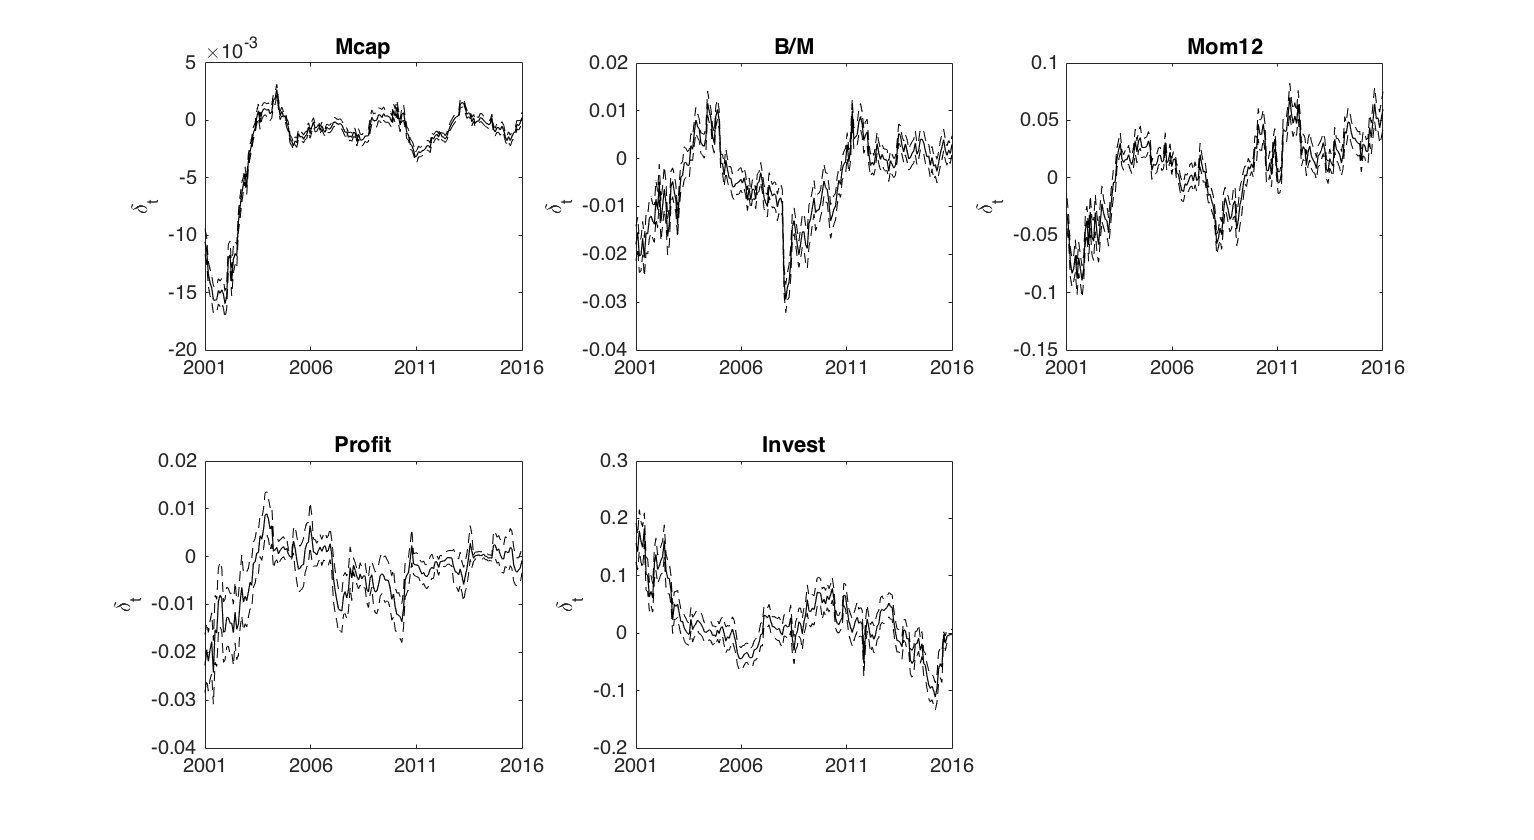
\includegraphics[width=18cm,height=10cm,\textwidth]{pictures/posterior_plots.png}
%   {\captionsetup{justification=centering,singlelinecheck=off}
% \caption{\bfseries Time series plots of the posterior means of the time-varying relation between six-factor alphas and characteristics $\delta_t$}  } 
% \caption*{The figure presents estimation results of the model in Eqs.(\ref{asset}), (\ref{cross}) and (\ref{delta_t}) examining the cross-sectional relation between six-factor alphas and all characteristics simultaneously. In each plot we report posterior results for a given characteristic across our sample period February 2001 to December 2016. The solid line is the posterior mean of $\delta_t$ and the dashed lines represent the 95\% credible interval.}
% \end{figure}
% \end{singlespacing}
% \vspace{-0.45cm}
\par Finally, we examine whether our results are robust to the risk factors included in Eq.(\ref{asset}). In Table \ref{table4} we add the posterior results from the model using alphas from the CAPM, the Fama-French three-factor model, the \citet{carhart1997persistence} four-factor model and the \citet{FAMA20151} five-factor model. The systematic relation between alphas and characteristics are similar across factor models. The posterior means of B/M, Mom12 and Invest vary the most across the factor models, indicating that cross-correlations are the largest between the value, momentum and investment effects, both through the risk factors and the characteristics. Interestingly, we find that the posterior mean of B/M changes sign when the quality factors are considered. The value factor in the three- and four-factor models under-adjusts for the value factor, as alphas are positively related to funds holding value stocks. Conversely, alphas from the five- and six-factor models are positively related to funds holding growth stocks. This contradiction is possibly caused by the interaction between the value factor and the quality factors, which is a negative correlation between the two. All in all, we conclude that the traditional Fama-French risk factors (jointly) insufficiently adjust returns for the main anomalies. 

%  \begin{singlespacing}
%  \begin{table}[h!]
% \small
% \centering
% \setlength{\tabcolsep}{16.5pt}
% {\captionsetup{justification=centering,singlelinecheck=off}
% \caption{\bfseries Multi-factor model alphas vs. characteristics }}
% \caption*{This table presents the results of the estimation of the model in Eqs.(\ref{asset}), (\ref{cross}) and (\ref{delta_t}) based on several Fama-French models. We employ the CAPM, the \citet{fama1993common} three-factor model, the \citet{carhart1997persistence} four-factor model, the \citet{FAMA20151} five-factor model and a six-factor model combining all factors. We estimate the model in each month during the period February 2001 to December 2016, using an estimation period of two years to estimate the factor model in Eq.(\ref{asset}), rolling the window a month at a time. 
%  The characteristics (Z) are the logarithm of market capitalization (Mcap), the logarithm of book-to-market ratio (B/M), the logarithm of one plus the past twelve-month cumulative return (Mom12), operating profitability (Profit) and asset growth (Invest). Each characteristic is standardized by subtracting the cross-sectional mean each month. We report the posterior mean and standard deviation for the aggregate-level parameters in $\bar{\delta}$, based on the posterior distribution of the parameters constructed from 5000 iterations of the Gibbs sampler with the first 2500 iterations discarded as a burn-in period. Estimates in bold font indicates that the 95\% credible interval of the posterior distribution does not include zero. 
% }
% \begin{tabular}{lrrrrr}
% \hline
% \multicolumn{1}{l}{} & \multicolumn{1}{l}{CAPM} & \multicolumn{1}{l}{FF 3FM} & \multicolumn{1}{l}{Carhart 4FM} & \multicolumn{1}{l}{FF 5FM} & \multicolumn{1}{l}{FF 6FM} \\ \hline
% Cnst & 0.000 & \textbf{-0.004}     & \textbf{-0.003}     & \textbf{-0.003}  & \textbf{-0.002} \\ & (0.000) & (0.000)& (0.000) & (0.000) & (0.000) \\ 
% Mcap                 & \textbf{-0.003}          & \textbf{-0.001}                     & \textbf{-0.001}                 & \textbf{-0.002}                     & \textbf{-0.002}                     \\
%                      & (0.000)                   & (0.000)                              & (0.000)                          & (0.000)                              & (0.000)                              \\
% B/M                  & \textbf{0.006}           & \textbf{0.002}                     & \textbf{0.001}                 & \textbf{-0.003}                     & \textbf{-0.003}                     \\
%                      & (0.001)                   & (0.000)                              & (0.000)                          & (0.001)                              & (0.000)                              \\
% Mom12                & \textbf{0.015}           & \textbf{0.008}                      & \textbf{0.004}                  & \textbf{0.007}                      & \textbf{0.005}                      \\
%                      & (0.003)                   & (0.003)                              & (0.003)                         & (0.003)                             & (0.003)                              \\
% Profit               & 0.003                    & 0.001                             & 0.001                          & -0.004                              & -0.003                           \\
%                      & (0.001)                   & (0.001)                              & (0.001)                          & (0.001)                              & (0.002)                              \\
% Invest               & \textbf{-0.046}          & \textbf{-0.023}                     & \textbf{0.020}                  & \textbf{0.014}                      & \textbf{0.017}                      \\
% \multicolumn{1}{l}{} & (0.005)                   & (0.004)                              & (0.004)                          & (0.004)                              & (0.004)                              \\ \hline
% \end{tabular}
% \end{table}
%  \end{singlespacing}

% There are many alternatives to evaluate the performance of mutual funds. A common performance measure is a fund's alpha, the return adjusted for exposures to risk factors that drives most of the fund's return. The typical approach is to regress fund returns onto a set of risk factors. The intercept (alpha) is then interpreted as the abnormal return reflecting the ability of the fund manager. Conventionally, the risk factors are the benchmark portfolio returns of Fama-French, which reflect the main anomalies in the cross-section of returns.  Alternatively, funds are evaluated relative to the characteristic-based benchmark approach of Daniel, Grinblatt, Titman, and Wermers (DGTW; 1997). The DGTW characteristic selectivity (CS) measure controls for the main anomalies by adjusting each fund position relative to the average return of a portfolio holdings stocks with similar characteristics.
% \par Both performance measures stand out for their simplicity, intuitive interpretation and widespread use. The parsimonious structure of both performance measures, however, has it drawbacks. \citet{huij2009use} argue that the Fama-French risk proxies are based on hypothetical stock portfolios that do not incorporate transaction costs, trade impact and trading restrictions, such that the resulting performance estimates for funds may be biased. They propose to use risk factors based on fund returns rather than stock returns to assess fund managerial skill. The DGTW CS measure is based on characteristic-based benchmarks, which are based on coarse quintile sorts to ensure well-populated benchmark portfolios. This might pose a problem when adjusting for multiple anomalies, especially for holdings with extreme characteristics. 
% \par \citet{brennan1998alternative} was the first to look beyond a unilateral explanation of cross-sectional variation in expected returns by either factor betas or characteristics. They find that characteristics (e.g., size, book-to-market, momentum) remain significantly related to expected returns even after the risk-adjustment by a factor model with risk factors based on those same characteristics. In addition, \citet{busse2017double} show that fund-level characteristics yield explanatory power over the cross-section of fund returns after controlling for exposures to the Fama-French risk factors. In Section \ref{section3}, we find that factor betas and fund-level characteristics equally contribute to the explained variation of fund returns. Therefore, we investigate several performance measures which adjusts for both.  

% \subsection{Double-adjusted alpha}
% \label{section4A1}
% For each fund $i$, we estimate the Fama-French six-factor model over a 36-month estimation period, rolling the window a month at a time. This results, given $N_t$ individual funds in month $t$, into a $N_t$ x 1 vector of estimated six-factor alphas $\hat{\alpha}_t$.
% Following \citet{brennan1998alternative}, the estimated alphas constitute the raw material which serves as the dependent variable in monthly cross-sectional regressions\footnote{As opposed to cross-sectional regressions in Section \ref{section3}, the measurement error in the factor betas $\hat{B}$ only effects the dependent variable in Eq.(\ref{double}), and while the factor betas are most probable to be correlated with the characteristics $Z$, there is no a priori reason to expect that the error term $u$ is correlated with the characteristics, such that the estimated coefficients $c$ are unbiased under the null hypothesis. While the EIV-bias is avoided since the estimated betas do not serve as explanatory variables, working with risk-adjusted returns has an important drawback. As noted in \citet{brennan1998alternative}, the risk-adjustment imposes the restriction that the zero-beta rate equals the risk-free rate and the risk premia are constrained to equal the factor means.}
% \begin{equation}
%     \label{double}
%     \hat{\alpha}_{i,t} = c_{0t} + c_{1t}Z_{it-1} + u_i, 
% \end{equation}
% where $Z_{it-1}$ are the lagged fund-level characteristics of fund $i$, $c_{0t}$ measures the average skill across funds in month $t$, $c_{1t}$ measures the rewards of the characteristics with respect to the fund's alpha, and $u_i$ is the idiosyncratic skill of fund $i$. The subscript $t$ for $\hat{\alpha}_{i,t}$ indicates that it is an estimate based on returns up until time $t$. The fund-level characteristics (Z) include the logarithm of market capitalization (Mcap), the logarithm book-to-market ratio (B/M), six-month cumulative return (Mom6), operating profitability (Profit), and investment (Invest). Before including them in the regressions, each characteristic is standardized by subtracting its the cross-sectional mean and dividing by the cross-sectional standard deviation in each month.  
% \par We compute an extended version of the double-adjusted performance measure
% % \footnote{\citet{busse2017double} apply the double-adjusted measure to mutual funds and adjust for size, value, and momentum effects. They propose two different approaches to calculate the double-adjusted measure. Next to the cross-sectional regression approach (used in this paper), they assign funds into portfolios based on a three-way sort on fund-level characteristics, and compare a fund's alpha to the average alpha of the characteristic-based portfolio to which the fund is assigned to. They find that using the portfolio approach does not materially differ the results.} 
% of \citet{busse2017double}. Using the estimated coefficients from Eq.(\ref{double}), the double-adjusted alpha is calculated as 
% \begin{equation}
%     \label{double_alpha} 
%     \alpha^{double}_{i,t} = \hat{\alpha}_{i,t} - c_{1t}Z_{it-1} = c_{0t} + u_i.
% \end{equation} 
% This double-adjusted measure captures performance attributable to fund exposures to risk factors, and also controls for the effects of stocks characteristics, such that we can better capture true fund managerial skill. Beginning with the 36th month during our sample, we compute double-adjusted alphas in each month from the period April 1983 to December 2015, consisting of 393 months. 
% \par Table 4 presents the effects of the adjustment of six-factor alphas for characteristics. Table A2 in the Appendix presents the results using the four-factor model of \citet{carhart1997persistence}. First, we compute average alphas in quintiles sorted on Mcap, B/M, Mom6, Profit or Invest. Each month $t$, we sort funds on lagged characteristics and compute the average alpha for each characteristic quintile. Panel A of Table 4 reports the time series mean of the average six-factor alpha in the characteristic quintiles. The results indicate that for sorts associated with B/M, Mom6 and Invest, the difference between the top quintile and the bottom quintile is statistically significant at the 5\% level. Funds in the top quintile have annualized alphas that are 0.94\% and 1.63\% higher than funds in the bottom quintile for sorts on Mom6 and Invest, respectively, while there is a negative annualized alpha spread of 1.88 for the sort on B/M. There is not a clear pattern across the quintiles sorted on Mcap and Profit. 
% \par Recall that the six-factor model adjust returns for exposures to factors based on Mcap, B/M, Mom6, Profit, and Invest. The results in Panel A of Table 4 suggest that the six-factor model under-adjusts for exposures to the momentum factor, while the model appears to over-adjust for influences related to the value and investment factors. In other words, funds holding high-momentum stocks show higher abnormal return despite the risk-adjustment to the WML factor. Conversely, funds holding positions in high book-to-market and conservative investment stocks under perform, contradictory to previous findings on value and investment effects. Similar conclusions were drawn by \citet{huij2009use}, which find that fund managers following a value-orientated strategy earn a substantially lower premium than those projected by the hypothetical hedge portfolio HML, while the momentum premium earned by funds is larger than that projected by the WML factor.
% \par Furthermore, to provide another indication of the relation between alphas and characteristics, Panel B of Table 4 reports the time-series average of monthly coefficients estimated from Eq.(\ref{double}). We report the average coefficients in univariate regressions with each characteristic and in a joint model. We also calculate \citet{fama1973risk} t-statistics calculated using standard errors with the \citet{newey1986simple} correction of 12 lags\footnote{\citet{petersen2009estimating} has modified the \citet{newey1986simple} correction to accommodate panel data.}. This correction is necessary since the dependent variable in the Fama-MacBeth regressions are derived from overlapping rolling windows. The univariate regressions indicate that there is a statistically significant relation at the 5\% level between alphas and all characteristics except Profit. In a multivariate setting only Invest remains statistically significant. In line with the results of the quintile sorts, the standard factor model benchmark returns for the momentum factor is too low, while the benchmark return is set too high for the value and investment factors. 

% \subsubsection{Double-adjusted DGTW characteristic selectivity measure}
% We extend the characteristic selectivity (CS) measure of  Daniel, Grinblatt, Titman, and Wermers (DGTW; 1997) by also adjusting for profitability and investment effects. We use benchmark returns of portfolio of stocks which is matched to the fund's holdings each quarter along the dimensions of size, value, momentum, profitability, and investment. Specifically, the DGTW CS measure of fund $i$ at time $t$ is calculated as 
% \begin{equation}
%     \label{DGTW_t} 
%     \text{DGTW}_{it} = \sum_{j=1}^{N_{it}} w_{jt-1}(R_{jt}-R^{j}_{t}), 
% \end{equation}
% which is simply the portfolio-weighted average of excess returns over the contemporaneous characteristic-based benchmark portfolio return $R^j_t$ across all holdings $j$ = 1,..., $N_{it}$. Appendix B describes the construction of the benchmark portfolios and how fund holdings are matched to these benchmarks. A DGTW CS value of 0 indicates that the performance of a fund could have been replicated, on average, by simply buying stocks with the characteristics as those held by the fund, and a positive DGTW CS value suggests additional stock-picking skills by the fund's manager. 
% \par Similar to double-adjusted alpha in Section \ref{section4A1}, we conduct an additional adjustment, now for a fund's factor betas. For each fund $i$ in month $t$, we calculate the DGTW CS measure from time $t$-35 until $t$, and calculate the time-series average over this period, which we denote by $\text{DGTW}_{i,t-35:t}$. We estimate the six-factor model over the same period and store the estimated betas $\hat{B}_{it}$. We conduct monthly cross-sectional regressions 
% \begin{equation}
% \label{double1}
%     \text{DGTW}_{i,t-35:t} = c_{0t} + c_{1t}\hat{B}_{it} + u_i,
% \end{equation}
% where $c_{0t}$ measures the average characteristic selectivity skill across funds in month $t$, and $c_{1t}$ measure the rewards of the fund factor betas with respect to the fund's DGTW CS measure, and $u_i$ is the idiosyncratic characteristic selectivity skill of fund $i$. Before including them in the regression, each factor beta is standardized by subtracting its monthly cross-sectional mean. 
% \par Using the estimated coefficients from Eq.(\ref{double1}), we adjust the DGTW CS measure for factor betas as 
% \begin{equation}
%     \label{double_DGTW}
%     \text{DGTW}^*_{i,t-35:t} = \text{DGTW}_{i,t-35:t} - c_{1t}\hat{B}_{it} = c_{0t} + u_i. 
% \end{equation}
% This double-adjusted measure first adjusts performance for stock characteristic effects, and in the second pass regression for exposures to factor betas. If the DGTW CS measure fully adjusts performance for the main anomalies, the factor betas should not convey information about the DGTW CS measure, such that the estimated coefficients $c_{1t}$ are indistinguishable from zero. We compute the double-adjusted DGTW CS measure in each month over from the period April 1983 to December 2015. 
% \par Table 5 presents the effects of the adjustment of the DGTW CS measure for factor betas. Table A3 in the Appendix presents the results when only adjusting for size, value, and momentum effects. First, we compute average DGTW CS measures in quintiles sorted on the six-factor betas, including MKRF (market factor), SMB, HML, WML, RMW, and CMA. Each month $t$, we sort funds on contemporaneous betas and compute the average DGTW CS value for each beta quintile. Panel A of Table 5, reports the time series mean of the average DGTW CS value in the beta quintiles. We find a distinct pattern across quintiles sorted on the SMB and WML betas, as the average DGTW CS measure increases nearly monotonically across the SMB and WML quintiles and indicates a sizable spread of 0.057 (t = 2.32) and 0.124 (t = 6.71) between the top and bottom quintiles of SMB and WML, respectively. Regarding quintiles sorted on HML, RMW, or CMA, the top-minus-bottom DGTW CS measures are, on average, indistinguishable from zero. 
% \par Panel B of Table 5 reports the time-series average of monthly coefficients estimated from Eq.(\ref{double1}), with \citet{fama1973risk} t-statistics calculated using standard errors with the \citet{newey1986simple} correction of 12 lags. Again, we find that SMB and WML betas are significantly related to the cross-section of DGTW CS measures, suggesting that the characteristic-based benchmark approach under-adjusts for size and momentum effects. We find statistical insignificant coefficients for the HML, RMW, and CMA betas, indicating that exposures to the value, profitability, and investment factors do not convey new information after the characteristic-based adjustment. 

% \subsection{Bayesian alphas }
% We employ the hybrid approach of \citet{cosemans2015estimating} for estimating factor betas that incorporate fund-level characteristics as prior information. This method relates to the asset pricing literature which condition factor betas on firm fundamentals and economic state variables. Previous literature including the works of \citet{lewellen2010skeptical}, \citet{avramov2006asset}, \citet{chordia2012cross} provide empirical evidence that factor betas are related to firm characteristics such as market capitalization and book-to-market ratios. By incorporating cross-sectional information on factor betas we may increase the accuracy of sample estimates since factor betas might be similar across funds with overlapping holdings. For illustration, consider we estimate a momentum beta of 0.1 for a fund with limited return data. However, based on the funds with similar holdings we find that momentum betas are normally distributed with moments equal to 0.2 and 0.4. Based on this information the sample estimate of 0.1 might be biased downwards.
% \par For each fund $i$, we conduct rolling-window estimations (window size of $\tau$ = 36 months) of the Fama-French six-factor model  

% \begin{equation}
%     \label{factor_model6}
%     R_{it} = \alpha_i + \beta_{i1}F_{1t} + ... + \beta_{i6}F_{6t} + \epsilon_{it} = \alpha_{i,t} + \beta'_{i,t} F_t + \epsilon_{it}, \hspace{0.2cm} t = t-\tau,...,t,
% \end{equation}
% where $R_{it}$ denotes excess monthly returns of fund $i$ and $F_t$ = [$F_{1t}$,...,$F_{6t}$] are the six-factor benchmark returns in month $t$, and $\epsilon_{it}$ is the residual return which is normally distributed with zero mean and variance $\sigma^2_{i,t}$. The subscript $t$ for $\alpha_{i,t}$ and $\beta_{i,t}$ indicates that we use monthly returns up until time $t$. To incorporate the fund-level characteristics as prior information, we use Bayesian techniques to estimate Eq.(\ref{factor_model6}). In the spirit of \citet{cosemans2015estimating}, we specify diffuse priors for alpha and the idiosyncratic variance $\sigma^2_{i,t}$ and assume a normal distribution for the prior of $\beta_{i,t}$, that is, 
% \begin{equation}
% \label{prior_beta}
%     p(\alpha_{i,t}) \propto 1, \hspace{0.2cm} p(\sigma^2_{i,t})  \propto \sigma^{-2}_{i,t} \hspace{0.2cm} \text{and} \  \hspace{0.2cm} \beta_{i,t} \sim \mathcal{N}(\bar{\beta}_{i,t},\Sigma_{\beta_{i,t}}). 
% \end{equation}
% The prior specification is unique to each fund for each month by including fund-specific information on the fund's holdings. In the next section we elaborate on how we determine the parameters in the prior of $\beta_{i,t}$. 
% \par We estimate the factor model using the Markov Chain Monte Carlo (MCMC) Gibbs sampler\footnote{Examples of Bayesian inference in asset pricing models are presented in \citet{mcculloch1990posterior} and \citet{harvey1990bayesian}. For an extensive reading on the application of the Gibbs sampler in econometrics, we refer to \citet{de2006gibbs}}. An attractive feature of MCMC techniques is that samples of random drawings can be generated from the joint posterior  indirectly, without the need to specify the exact form of this joint distribution directly. The Gibbs sampler uses an iterative procedure to create Markov chains by simulating from full conditional posteriors instead which are typically much easier to derive. After the Markov chains have converged, the sets of draws that are obtained from the conditional posteriors can be effectively considered as samples from the joint posterior. We describe the steps in the Gibbs sampler thoroughly in Appendix C. We use the posterior mean of $\alpha_{i,t}$ as our (double-adjusted) performance measure, which we denote as $\alpha^{Bayes}_{i,t}$.

% \subsubsection*{Prior estimation}
% We specify a monthly panel model to elicit a prior for factor betas of fund $i$ in month $t$, 
% \begin{equation}
% \label{panel1}
%     R_{it} = \alpha^*_i + \beta^*'_{i,t|t-1}F_t + \eta_{it}, 
% \end{equation}
% which is the same model as in Eq.(\ref{factor_model6}), but now using the entire panel rather than fund-specific over rolling windows. The idiosyncratic return $\eta_{it}$ is normally distributed with zero mean and variance $\sigma^2_{\eta_i}$ and is assumed to be independent across funds. We define prior beta as follows
% \begin{equation}
% \label{con_beta}
%     \beta^*_{i,t|t-1} = \delta_i + \xi' Z_{it-1}, 
% \end{equation}
% where each factor beta is parameterized as a linear function of lagged fund-level characteristics (Z). The fund-level characteristics (Z) include the logarithm of market capitalization (Mcap), the logarithm book-to-market ratio (B/M), six-month cumulative return (Mom6), operating profitability (Profit), and investment (Invest). Before including them in the regressions, each characteristic is standardized by subtracting its the cross-sectional mean and dividing by the cross-sectional standard deviation in each month. 
% \par In the panel model the regression constant $\delta_i$ = [$\delta_{i1},...,\delta_{i6}$]' is unique to each fund, while the loadings on the characteristics are pooled in $\xi$ = [$\xi_1$,...,$\xi_6$]. The fund-specific parameters mitigates the omitted variable bias by accounting for effects on beta which are constant but vary across funds. The pooled parameters increase estimation precision by using cross-sectional information from the entire sample, as we expect there exists a generic relation between factor betas and characteristics across funds. 
% \par Given the specification of the prior beta, substitution of Eq.(\ref{con_beta}) in Eq.(\ref{panel1}) and some rewriting yields
% \begin{equation}
% \label{panel}
%     R_{it} = \alpha^*_i + (\delta_{i1} + \xi_1'Z_{it-1})F_{1t} + ... + (\delta_{i6} + \xi_6'Z_{it-1})F_{6t} + \eta_{it}.
% \end{equation}
% We use the MCMC Gibbs sampler to estimate Eq.(\ref{panel}), as this Bayesian approach allows let some parameters vary across funds to capture unobserved heterogeneity in factor betas, while pooling other parameters to exploit cross-sectional information.  Using the estimates from the panel model we can compute posterior results for $\beta^*_{i,t|t-1}$, which constitute the prior mean and variance for $\beta_{i,t}$ in Eq.(\ref{prior_beta}). We describe the steps in the Gibbs sampler thoroughly in Appendix D.

% \subsection{Importance of adjustment for characteristics}
% \label{importance}
% To provide initial evidence that the standard factor model alpha imperfectly controls for passive loadings on characteristics, we examine the Fama-French six-factor alpha of funds sorted into quintiles based on the fund-level market capitalization, book-to-market ratio, past twelve-month cumulative return, operating profitability, and investment. During the sample period April 1983 to December 2015, we estimate each month the six-factor model alpha over the past 36 months. We then funds into deciles based on fund-level characteristics averaged over the past 36-month window, lagged one month, and we compute the average standard alpha in each characteristic decile. 
% \par Table 4 reports the average six-factor alpha in the characteristic decile. The results indicate that for sorts associated with B/M, Mom6 and Invest, the difference between the top decile and the bottom decile is statistically significant at the 5\% level. Funds in the top decile have annualized alphas that are 1.20\% and 1.17\% higher than funds in the bottom decile for sorts on Mom6 and Invest, respectively, while there is a negative annualized alpha spread of 1.31\% for the sort on B/M. There is not a clear pattern across the deciles sorted on Mcap and Profit. 
%  \par Recall that the six-factor model adjusts returns for exposures to factors based on Mcap, B/M, Mom6, Profit, and Invest. The results in Table 4 suggest that the six-factor model under-adjusts for exposures to the momentum factor, while the model appears to over-adjust for influences related to the value and investment factors. In other words, funds holding high-momentum stocks show higher abnormal return despite the risk-adjustment to the WML factor. Conversely, funds holding positions in high book-to-market and conservative investment stocks under perform, contradictory to previous findings on value and investment effects. Similar conclusions were drawn by \citet{huij2009use}, which find that fund managers following a value-orientated strategy earn a substantially lower premium than those projected by the hypothetical hedge portfolio HML, while the momentum premium earned by funds is larger than that projected by the WML factor.
%  \par Furthermore, Table 5 reports the estimated loadings on characteristics from the panel regression model in  Eq.(\ref{double_alpha}). We compute the average regression coefficients across all sample months. We also calculate \citet{fama1973risk} t-statistics calculated using standard errors with the \citet{newey1986simple} correction of 12 lags.\footnote{\citet{petersen2009estimating} has modified the \citet{newey1986simple} correction to accommodate panel data.} This correction is necessary since there is overlap in the estimation windows. The results in Table 5 show that, on average, fund returns are sensitive to the characteristics of the stocks held in fund portfolios. All characteristics but Invest yield a statistically significant relation at the 5\% level with fund returns. 
 
%  \subsection{Effects of double adjustment}
%  The results in Section \ref{results} demonstrate that the characteristics of the holdings of funds are an important determinant of expected fund returns. In Section \ref{importance} we have demonstrated an important shortcoming of the standard factor models, insofar as they attribute skill to passive exposures to characteristics. We have proposed a new performance measure which accounts for the performance attributable to characteristics to produce a purer quantification of skill. In this section we investigate whether our double-adjusted performance measure adequately adjusts performance to characteristics. We also examine whether our performance measure materially impacts fund percentile performance rankings relative to using the standard factor model alpha. 
%  \par Similar to the previous section, we sort funds into deciles based on  fund-level characteristics averaged over the past 36-month period, lagged one month. For each month in our sample we compute the average double-adjusted performance measure for each characteristic decile. Table 6 shows that the top-minus-bottom spread in alpha is statistically indistinguishable from zero for each characteristic sort. For the sorts on B/M and Mom12 we still find a similar pattern in double-adjusted alpha as with standard alpha, but the characteristic-adjustment seems to have mitigated these patters. Thus, the new performance measure is less sensitive to passive loadings on characteristics, such that performance attributable to characteristics is mostly removed from our double-adjusted alpha. 
%  \par One might anticipate that the new performance measure could alter the performance ranking of funds. In each month in our sample, we sort funds into percentiles based on double-adjusted alpha and on standard six-factor alpha. Table 7 presents the distribution of the difference in percentile rankings. When we compare percentile performance rankings between the two performance measures, we find that the median change in percentile rankings is 8.67\%. Moreover, many funds exhibit dramatic changes in performance rank, with 25 (10) of funds experiencing a mean change in percentile ranking of at least 16.25\% (25.47\%). 
 
% \subsection{Effects of adjustment alpha for characteristics}
% The results in Section \ref{section4b} indicate that the standard factor models provide inadequate risk-adjustments to the common risk factors. As a consequence, alpha does not fully reflect performance in excess of risk factors as it attributes skill to passive exposure to characteristics underlying these factors. Double-adjusted alpha rectifies this by providing a performance measure corrected for exposures to both risk factors and underlying characteristics. First, we investigate whether the adjustment for characteristics materially differs the performance ranking of funds. Second, we conduct a battery of simulations to examine whether the double-adjusted performance measure is better at identifying stock-picking skill. 
% \par 
% Specifically, we rank funds each month in percentiles according to their alphas and double-adjusted alphas, and compare the differences between the performance percentile rankings. Figure 1 shows the absolute differences between performance percentile rankings caused by adjusting alpha for characteristics. Funds experience a median change in percentile rank of about five percent when adjusting alpha. That is, a fund that ranks in the 50th percentile based on alpha ranks in the 45th or 55th percentile with the characteristics adjustment. Moreover, we find that 25 percent of funds experience a change in percentile ranking of at least 10 percent.
% \subsubsection*{Simulations}
% For the simulations, we follow the framework set by \citet{busse2017double}. The goal of the simulations is to assess whether the performance measures can distinguish skill from luck. We simulate fund returns with zero stock-picking skills by design and compute the standard factor alpha and the double-adjusted alpha. The superior performance measure identifies no skill across simulated funds, which should result in marginal cross-sectional differences in alpha. The bootstrap simulations of \citet{busse2017double} are similar to the simulations in \citet{kosowski2006can} and \citet{fama2010luck}, which investigate skill in the cross-section of fund returns. 
% \par 
% We simulate funds returns by repeatedly constructing a fund's portfolio by sampling stocks from the actual data. For each fund in the sample, we create a simulated fund portfolio with holdings similar to the actual fund's portfolio, in terms of the fund's TNA, number of holdings, portfolio weights and the characteristics of each holding. First, each month we sort the funds in the actual sample into quintiles based on funds' TNA. Within each fund size group, we record all the unique stocks held by all funds, and we assign each stock into quintiles for each stock characteristic. 
% \par 
% We simulate a fund's portfolio as follows. For each fund at a given report date, we randomly select a stock for each position in the fund's portfolio from a list of stocks matching the fund's size ranking. We further narrow down the list of stocks to those matching the  quintile rankings of the given position. To the stocks in the final list we assign sampling probabilities equal to the number of funds holding each stock. The number of shares held of a simulated position equals the initial investment of the original position divided by the price of the simulated position at the report date. We maintain this simulated portfolio in subsequent months up until the next report date with a maximum holding period of three months. We compute a fund's portfolio-weighted gross return using portfolio weights based on the number of shares (determined at the report date) and the returns (from the actual data) of the simulated stocks\footnote{Fund returns in the CRSP Mutual Fund Database are reported net of all operating expenses (expense ratio). \citet{carhart1997persistence} show that expense ratios are negatively related with net returns. \citet{wermers2000mutual} use fund holdings to decompose gross fund returns into several components and show that stock-picking skills of fund managers are masked by expense ratios. By using gross returns derived from the fund's holdings in the simulations, we can better measure skill across funds.  }. 

\newpage
\section{Impact on Relative Mutual Fund Performance}
 
\label{relative_performance}
In Section \ref{section2C}, we show the importance of incorporating characteristics in explaining the returns of mutual funds. The results in the previous section demonstrate an important flaw of the traditional factor model alphas, insofar as they attribute skill to passive exposures to characteristics. Therefore, we propose a mutual fund performance measure which adjusts performance for exposures to both factor betas and characteristics. 

In this section, we examine the extent to which our new double-adjusted alpha affects inference relating to relative mutual fund performance. We replicate the work of several mutual fund performance studies using  six-factor alpha as our baseline measure of performance, computed  using the traditional time series regression approach.\footnote{Even though the hierarchical Bayes model also provides estimates of fund alphas, we choose the time series regression approach as this is standard in previous literature. Moreover, the Bayesian estimate of standard alpha makes use of cross-sectional information. To highlight the difference made by adjusting performance for characteristics, we compare our double-adjusted alpha to a performance measure which is not influenced by these characteristics.} Because we use traditional alpha as our baseline performance measure, we can  easily extend previous analysis with the two components of alpha, our double-adjusted measure and the portion of alpha associated with characteristics (see Eqs.(\ref{double_adjusted_alpha}) and (\ref{char})). The decomposition of alpha will indicate the extent to which both components contribute to the main findings of previous studies.\footnote{We follow \citet{busse2017double} in reassessing previous findings in the mutual fund literature using the double-adjusted performance measure. In addition to the analyses in this paper, they also reevaluated the relation between fund performance and the industry concentration \citep{kacperczyk2005industry}, the return gap \citep{kacperczyk2008unobserved}, and active share \citep{cremers2009active}.  } 

We begin by calculating the difference in fund percentile performance rankings between using double-adjusted alpha in comparison to those based on alpha. Next, central to the mutual fund performance literature are studies that analyze persistence in fund performance, e.g., \citet{carhart1997persistence}. Other studies examine the relation between fund performance and certain fund features, such as a fund's factor model R-squared \citep{amihud2013mutual} and a fund's investors cash flows \citep{barber2016factors}. We plug in our estimates of the posterior mean of both components of alpha in the analysis of these papers. We use the estimation methods used in these papers to accommodate a fair comparison between inferences based on traditional alpha and those based on double-adjusted alpha.

\subsection{Relative Mutual Fund Performance Rankings}
We examine the degree to which our new performance measure alters the performance rankings of funds. In each month in our sample, we sort funds into percentiles based on six-factor alpha ($\alpha$) and on double-adjusted six-factor alpha ($\alpha^*$). Given a number of $N_t$ funds in month $t$, we obtain pairs of percentile ranks for each fund $\{(P^{\alpha}_{1t},P^{\alpha^*}_{1t}),..., (P^{\alpha}_{N_tt},P^{\alpha^*}_{N_tt})\}$. Using the percentile rank pairs we compute Kendall's tau coefficient, which is a correlation coefficient between two rankings. We find a time series average of Kendall's tau equal to 0.70, which indicates differences between the two rankings. 

To examine the impact of double-adjusted alpha on performance rankings in more detail, we compute the difference between the performance ranks $P^{\alpha}_t$ and $P^{\alpha^*}_t$ for each fund in each month $t$. Table \ref{table5}
presents the time series average distribution (across all months in our sample) of the difference in percentile performance rankings. We find that the median change in percentile rankings is roughly 9\%, i.e., a fund which is ranked in the median percentile according to alpha is ranked in either the 41th or 59th percentile based on double-adjusted alpha. Moreover, many funds exhibit dramatic changes in percentile ranking, with 10 (5) percent of funds exhibiting a mean change in percentile ranking of at least 22.99\% (27.24\%). Thus, we find that adjusting traditional alpha for characteristics materially impacts the performance ranking of funds.

% \begin{singlespacing}
% \begin{table}[H]
% \small
% \centering
% \setlength{\tabcolsep}{12.5pt}
% {\captionsetup{justification=centering,singlelinecheck=off}
% \caption{\bfseries Change in performance percentile rankings  }}
% \caption*{This table presents the differences between the performance percentile ranks based on double-adjusted six-factor alpha ($\alpha^*$) relative to six-factor alpha ($\alpha$). These performance measures are calculated using rolling windows with a window size of 24 months (see section \ref{double_alpha}). Each month in our sample period we compute the difference between the percentile ranking based on alpha ($P^\alpha$) and the percentile ranking based on double-adjusted alpha ($P^{\alpha^*}$). We report the time series average distribution of the difference between performance rankings. The sample period is February 2001 to December 2016.}
% {\captionsetup{justification=centering,singlelinecheck=off}

% \label{my-label}
% \begin{tabular}{crrrrrrr}
% \hline
% Percentile     & 5      & 10     & 25    & 50   & 75    & 90    & 95    \\ \hline
% Rank (\%)   &  -22.93 & -17.89 &	-8.99 &	-0.02 &	9.05 & 17.84 &	23.07 \\
% Abs. Rank (\%) & 0.99 & 	1.49 & 	4.08 &	9.03 &	15.98 & 	22.99 &	27.24\\ \hline
% \end{tabular}
% \end{table}
% \end{singlespacing}

\subsection{Mutual Fund Return Persistence}
Mutual fund persistence is well documented in the finance literature. Early works include \citet{grinblatt1992persistence}, \citet{brown1995performance} and \citet{wermers1997momentum}, which document significant persistence in mutual fund rankings based on returns after adjustment for risk. This persistence lasts over horizons of one to three years, and they attribute the persistence to ``hot hands" or common investment strategies. \citet{carhart1997persistence} add stock momentum as an additional risk factor and find a significant difference in abnormal returns of more than 4\% on an annual basis. Drawing on Carhart's findings, \citet{bollen2004short} find an average abnormal return of 39 basis points for the top quintile in the post-ranking quarter. This post-ranking abnormal return disappears when evaluated over longer periods. 

We examine return persistence in several performance measures: six-factor alpha ($\alpha$), double-adjusted six-factor alpha ($\alpha^*)$ and characteristic-driven performance ($\alpha^{char}$). If our new performance measure, which accounts for characteristics, is a better indicator of true skill, we expect double-adjusted alpha to account for most of the persistence in alpha, such that double-adjusted alpha persists for a longer period. In this case, there should be no distinct return pattern using characteristic-driven performance. That is, if true skill goes beyond the premiums which are passively associated with characteristics. 

We replicate the studies on return persistence.\footnote{This paper adopts a similar approach to the one used in \citet{carhart1997persistence}. The only difference is the frequency of rebalancing, which is set to a quarterly basis in this work. \citet{busse2017double} analyzed persistence in their double-adjusted performance measure. They adopt an annual rebalancing of portfolios and found new evidence of persistence in mutual fund skill based on their double-adjusted performance measure.} Each quarter-end, we sort funds into deciles using the aforementioned performance measures; decile 10 contains the best performing funds and decile 1 contains the worst performing funds. We hold the sorted portfolios for up to six years and compute the equal-weighted return in each decile in the post-ranking period. To deal with overlapping decile portfolios formed in different quarters, we compute the equal-weighted return across overlapping periods. We examine the post-ranking performance by concatenating the returns of all post-ranking periods for each decile and estimate six-factor alpha using the resulting time series of post-ranking (monthly) returns for each decile. 

Table \ref{table6} presents the persistence results. Panel A shows strong evidence of persistence in standard six-factor alpha. In the short term, the average difference in alpha between the top and bottom deciles is 0.28 (t = 3.62) in the following quarter and 0.27 (t = 3.85) in the year thereafter, both of which significant from a statistical and an economic perspective. This abnormal return difference remains statistically significant in the second and third year after formation, followed by a decrease in the top-minus-bottom post ranking abnormal return from the fourth year onwards. Consistent with the findings of \citet{carhart1997persistence}, we find that the majority of the return spread is driven by past losing funds in the bottom deciles. In untabulated results, we find significant negative alphas in the bottom decile with t-statistics below -3. 

The results in Panel B show strong evidence that the double-adjusted six-factor alpha predicts future fund performance. We find a distinct return pattern across deciles sorted on our double-adjusted performance measure, as post-ranking alpha increases nearly monotonically across deciles and indicates a sizable return spread of 0.19 (t = 5.31) in the post-ranking quarter. The top-minus-bottom portfolios yield statistical significant alphas between 0.05 and 0.17, which persist up to six years. In Figure \ref{figure2}, we analyze return persistence on the long term. We graph the cumulative six-factor alpha of the top-minus-bottom portfolios, where the three plots lines represent alternative sorts on six-factor alpha, double-adjusted six-factor alpha, and characteristic-driven performance. The plots indicate an upward trend in the cumulative performance of both alpha and double-adjusted alpha, which lasts for the entire holding period of ten years. The results in Panel B of Table \ref{table6} combined with the plots from Figure \ref{figure2} suggest that double-adjusted alpha reflects true skill, which pays off in the long run such that persistence in this component of alpha causes most of the persistence in alpha. Our results are in line with the persistence analysis in \citet{busse2017double}. Using their double-ajdusted alpha they find evidence of persistence in fund four-factor alphas up to nine years after the initial ranking. We show that persistence is also present when a shorter sample period is used. 

In Panel C of Table \ref{table6} we turn to the component of alpha driven by passively loading on characteristics. The average return difference in alpha in the first year after formation is 0.16 with insignificant t-statistics, followed by a slight reversal from the second year onwards. The graph in Figure \ref{figure2} shows that sorts on characteristic-driven performance does not exhibit a distinct return pattern after formation in the long term. These results indicate that returns associated with characteristics do not convey information about future fund performance. This supports the claim that evidence of return predictability in alpha is mostly accounted for by the component adjusted for passive loadings on characteristics. By removing this noisy component, which does not detect skill, double-adjusted alpha is a more precise measurement of skill, leading to stronger evidence of persistence in mutual fund performance. 


% \begin{singlespacing}
% \begin{table}[h!]
% \small
% {\captionsetup{justification=centering,singlelinecheck=off}
% \caption{ \bfseries Mutual fund performance persistence }}
% \caption*{This table presents returns of decile porfolios sorted by six-factor alpha (Panel A), double-adjusted six-factor alpha (Panel B) and characteristic-driven performance (Panel C). These performance measured are calculated using rolling windows with a window size of 24 months. Portfolios are rebalanced every quarter-end and are held for up to six years. To deal with overlapping portfolios, we follow \citet{jegadeesh1993returns} to take the equal-weighted return across overlapping portfolios formed in different quarters. Two different returns are reported: the excess return over the risk-free rate and the Fama-French six-factor alpha. T-statistics, shown in parenthesis, are computed using White's standard errors. Estimated significant at the 5\% level are in bold font. The sample period is May 1980 to December 2015.}
% \label{my-label}
% \begin{tabular}{crrrrrrrrrrr}
% \hline
%       & \multicolumn{2}{c}{Qtr 1}     &  & \multicolumn{2}{c}{Qtr 1-4}   &  & \multicolumn{2}{c}{Qtr 5-12}  &  & \multicolumn{2}{c}{Qrt 13-24} \\ \cline{2-3} \cline{5-6} \cline{8-9} \cline{11-12} 
% Decile & Excess        & 6F alpha      &  & Excess        & 6F alpha      &  & Excess        & 6F alpha      &  & Excess       & 6F alpha       \\ \hline
% \multicolumn{12}{l}{Panel A: Six-factor alpha}                                                                                                         \\
% 1      & 0.53          & -0.17         &  & 0.54          & -0.17         &  & 0.55          & -0.12         &  & 0.51         & -0.12          \\
% 2      & 0.56          & -0.08         &  & 0.56          & -0.09         &  & 0.55          & -0.10         &  & 0.55         & -0.07          \\
% 3      & 0.56          & -0.08         &  & 0.56          & -0.08         &  & 0.56          & -0.08         &  & 0.53         & -0.09          \\
% 4      & 0.56          & -0.08         &  & 0.56          & -0.08         &  & 0.57          & -0.07         &  & 0.52         & -0.09          \\
% 5      & 0.57          & -0.07         &  & 0.57          & -0.07         &  & 0.55          & -0.08         &  & 0.52         & -0.09          \\
% 6      & 0.57          & -0.06         &  & 0.56          & -0.06         &  & 0.53          & -0.09         &  & 0.53         & -0.08          \\
% 7      & 0.58          & -0.05         &  & 0.58          & -0.05         &  & 0.55          & -0.07         &  & 0.52         & -0.09          \\
% 8      & 0.59          & -0.05         &  & 0.58          & -0.06         &  & 0.55          & -0.08         &  & 0.52         & -0.08          \\
% 9      & 0.64          & -0.01         &  & 0.63          & -0.01         &  & 0.57          & -0.05         &  & 0.53         & -0.08          \\
% 10     & 0.68          & 0.01          &  & 0.66          & 0.00          &  & 0.60          & -0.04         &  & 0.55         & -0.08          \\
% 10-1  & 0.16          & 0.18          &  & 0.13          & 0.17          &  & 0.05          & 0.09          &  & 0.04         & 0.04           \\
%       & (\textbf{2.93}) & (\textbf{3.45}) &  & (\textbf{2.51}) & (\textbf{3.59}) &  & (1.16)          & (1.85)          &  & (1.19)         & (1.18)           \\
%       &               &               &  &               &               &  &               &               &  &              &                \\
% \multicolumn{12}{l}{Panel B: Double-adjusted six-factor alpha}                                                                                 \\
% 1      & 0.55          & -0.15         &  & 0.56          & -0.14         &  & 0.54          & -0.13         &  & 0.50         & -0.13          \\
% 2      & 0.57          & -0.09         &  & 0.55          & -0.11         &  & 0.55          & -0.10         &  & 0.52         & -0.10          \\
% 3      & 0.58          & -0.07         &  & 0.59          & -0.06         &  & 0.55          & -0.10         &  & 0.53         & -0.08          \\
% 4      & 0.55          & -0.08         &  & 0.57          & -0.07         &  & 0.56          & -0.07         &  & 0.51         & -0.10          \\
% 5      & 0.59          & -0.04         &  & 0.57          & -0.06         &  & 0.55          & -0.08         &  & 0.52         & -0.09          \\
% 6      & 0.56          & -0.06         &  & 0.55          & -0.07         &  & 0.54          & -0.08         &  & 0.52         & -0.09          \\
% 7      & 0.58          & -0.06         &  & 0.56          & -0.08         &  & 0.54          & -0.07         &  & 0.53         & -0.08          \\
% 8      & 0.59          & -0.05         &  & 0.60          & -0.04         &  & 0.57          & -0.05         &  & 0.53         & -0.08          \\
% 9      & 0.58          & -0.05         &  & 0.59          & -0.04         &  & 0.57          & -0.06         &  & 0.55         & -0.06          \\
% 10     & 0.68          & 0.01          &  & 0.66          & 0.00          &  & 0.60          & -0.04         &  & 0.55         & -0.08          \\
% 10-1  & 0.13          & 0.16          &  & 0.10          & 0.14          &  & 0.07          & 0.09          &  & 0.05         & 0.05           \\
%       & (\textbf{3.95}) & (\textbf{4.52}) &  & (\textbf{3.41}) & (\textbf{4.82}) &  & (\textbf{2.27}) & (\textbf{3.05}) &  & (1.84)         & (1.93)           \\ \hline
% \end{tabular}
% \end{table}

% \end{singlespacing}

% \begin{singlespacing}
% \begin{table}[h!]
% \small
% \centering
% {\captionsetup{justification=centering,singlelinecheck=off}
% \caption{ \bfseries Mutual fund performance persistence }}
% \caption*{This table presents the returns of decile porfolios sorted by six-factor alpha (Panel A), double-adjusted six-factor alpha (Panel B) and characteristic-driven performance (Panel C). These performance measures are calculated using rolling windows with a window size of 24 months (see section \ref{double_alpha}). Portfolios are rebalanced every quarter-end and are held for up to six years. To deal with overlapping portfolios, we follow \citet{jegadeesh1993returns} to take the equal-weighted return across overlapping portfolios formed in different quarters. Two different returns are reported: the excess (monthly) return over the risk-free rate and the Fama-French six-factor alpha. T-statistics, shown in parenthesis, are computed using White's standard errors. Estimated significant at the 5\% level are in bold font. The sample period is February 2001 to December 2016.}
% \label{my-label}
% \begin{tabular}{crrrrrrrrrrr}
% \hline
%       & \multicolumn{2}{c}{Qtr 1}         &  & \multicolumn{2}{c}{Qtr 1-4}       &  & \multicolumn{2}{c}{Qtr 5-12} &  & \multicolumn{2}{c}{Qtr 13-24} \\ \cline{2-3} \cline{5-6} \cline{8-9} \cline{11-12} 
% Decile & Excess          & 6F alpha        &  & Excess          & 6F alpha        &  & Excess   & 6F alpha          &  & Excess    & 6F alpha          \\ \cline{1-3} \cline{5-12} 
% \multicolumn{12}{l}{Panel A: Six-factor alpha ($\alpha$)}                                                                                                         \\
% 1    & 0.43   & -0.27         &  & 0.44   & -0.26         &  & 0.49   & -0.18         &  & 0.57 & -0.12  \\
% 2    & 0.46   & -0.20         &  & 0.45   & -0.21         &  & 0.49   & -0.15         &  & 0.56 & -0.10  \\
% 3    & 0.44   & -0.19         &  & 0.45   & -0.19         &  & 0.49   & -0.15         &  & 0.56 & -0.10  \\
% 4    & 0.47   & -0.16         &  & 0.47   & -0.16         &  & 0.49   & -0.13         &  & 0.56 & -0.10  \\
% 5    & 0.49   & -0.13         &  & 0.49   & -0.13         &  & 0.50   & -0.12         &  & 0.56 & -0.10  \\
% 6    & 0.53   & -0.09         &  & 0.52   & -0.11         &  & 0.54   & -0.10         &  & 0.57 & -0.09  \\
% 7    & 0.54   & -0.08         &  & 0.54   & -0.09         &  & 0.55   & -0.08         &  & 0.57 & -0.09  \\
% 8    & 0.57   & -0.06         &  & 0.56   & -0.07         &  & 0.56   & -0.08         &  & 0.59 & -0.08  \\
% 9    & 0.57   & -0.05         &  & 0.57   & -0.04         &  & 0.59   & -0.06         &  & 0.59 & -0.08  \\
% 10   & 0.58   & 0.01          &  & 0.58   & 0.01          &  & 0.57   & -0.06         &  & 0.58 & -0.08  \\
% 10-1 & 0.15   & \textbf{0.28} &  & 0.14   & \textbf{0.27} &  & 0.08   & \textbf{0.12} &  & 0.01 & 0.05   \\
%      & (1.63) & (3.62)        &  & (1.61) & (3.85)        &  & (1.14) & (2.17)        &  & 0.16 & (1.01)     \\
%       &                 &                 &  &                 &                 &  &          &                   &  &           &                   \\
% \multicolumn{12}{l}{Panel B: Double-adjusted six-factor alpha ($\alpha^*$)}                                                                                         \\
% 1    & 0.43          & -0.21         &  & 0.45          & -0.20         &  & 0.51   & -0.14         &  & 0.57   & -0.12         \\
% 2    & 0.48          & -0.18         &  & 0.49          & -0.17         &  & 0.52   & -0.13         &  & 0.57   & -0.10         \\
% 3    & 0.47          & -0.18         &  & 0.50          & -0.17         &  & 0.52   & -0.13         &  & 0.58   & -0.09         \\
% 4    & 0.48          & -0.17         &  & 0.49          & -0.15         &  & 0.52   & -0.13         &  & 0.56   & -0.10         \\
% 5    & 0.51          & -0.14         &  & 0.50          & -0.15         &  & 0.51   & -0.13         &  & 0.58   & -0.09         \\
% 6    & 0.53          & -0.11         &  & 0.52          & -0.12         &  & 0.54   & -0.11         &  & 0.58   & -0.09         \\
% 7    & 0.55          & -0.07         &  & 0.52          & -0.11         &  & 0.53   & -0.11         &  & 0.57   & -0.09         \\
% 8    & 0.51          & -0.11         &  & 0.53          & -0.09         &  & 0.53   & -0.09         &  & 0.56   & -0.10         \\
% 9    & 0.54          & -0.04         &  & 0.53          & -0.06         &  & 0.54   & -0.07         &  & 0.57   & -0.08         \\
% 10   & 0.57          & -0.02         &  & 0.56          & -0.03         &  & 0.55   & -0.05         &  & 0.59   & -0.07         \\
% 10-1 & \textbf{0.14} & \textbf{0.19} &  & \textbf{0.11} & \textbf{0.17} &  & 0.04   & \textbf{0.08} &  & 0.02   & \textbf{0.05} \\
%      & (3.81)        & (5.31)        &  & (3.17)        & (5.37)        &  & (1.34) & (2.94)        &  & (0.69) & (2.05)    \\ \hline
% \end{tabular}
% \end{table}
% \end{singlespacing}

% \begin{singlespacing}
% \begin{table}[h!]
% \small
% \centering
% {\captionsetup{justification=centering,singlelinecheck=off}
% \caption*{ \bfseries Table 6 (Continued) }}
% \label{my-label}
% \begin{tabular}{crrrrrrrrrrr}
% \hline
%       & \multicolumn{2}{c}{Qtr 1} &  & \multicolumn{2}{c}{Qtr 1-4} &  & \multicolumn{2}{c}{Qtr 5-12} &  & \multicolumn{2}{c}{Qtr 13-24} \\ \cline{2-3} \cline{5-6} \cline{8-9} \cline{11-12} 
% Decile & Excess     & 6F alpha     &  & Excess      & 6F alpha      &  & Excess       & 6F alpha      &  & Excess       & 6F alpha       \\ \hline
% \multicolumn{12}{l}{Panel C: Characteric-driven performance ($\alpha^{char}$)}                                                                       \\
% 1    & 0.48   & -0.18  &  & 0.44   & -0.22  &  & 0.47   & -0.15  &  & 0.58   & -0.09  \\
% 2    & 0.47   & -0.16  &  & 0.46   & -0.17  &  & 0.47   & -0.14  &  & 0.56   & -0.09  \\
% 3    & 0.46   & -0.16  &  & 0.45   & -0.16  &  & 0.48   & -0.13  &  & 0.55   & -0.10  \\
% 4    & 0.44   & -0.16  &  & 0.45   & -0.15  &  & 0.48   & -0.13  &  & 0.55   & -0.10  \\
% 5    & 0.42   & -0.18  &  & 0.44   & -0.15  &  & 0.50   & -0.12  &  & 0.55   & -0.11  \\
% 6    & 0.45   & -0.14  &  & 0.46   & -0.13  &  & 0.52   & -0.11  &  & 0.55   & -0.11  \\
% 7    & 0.52   & -0.10  &  & 0.52   & -0.10  &  & 0.55   & -0.09  &  & 0.58   & -0.10  \\
% 8    & 0.59   & -0.06  &  & 0.57   & -0.08  &  & 0.59   & -0.06  &  & 0.61   & -0.08  \\
% 9    & 0.62   & -0.05  &  & 0.62   & -0.05  &  & 0.60   & -0.08  &  & 0.61   & -0.07  \\
% 10   & 0.63   & -0.02  &  & 0.65   & -0.02  &  & 0.60   & -0.08  &  & 0.60   & -0.07  \\
% 10-1 & 0.15   & 0.16   &  & 0.20   & 0.20   &  & 0.13   & 0.07   &  & 0.02   & 0.02   \\
%      & (0.97) & (1.28) &  & (1.44) & (1.91) &  & (1.11) & (0.84) &  & (0.20) & (0.32)        \\ \hline
% \end{tabular}
% \end{table}
% \end{singlespacing}

% \begin{singlespacing}
% \begin{figure}[h!]
% \centering
%   \captionsetup{justification=left}
%   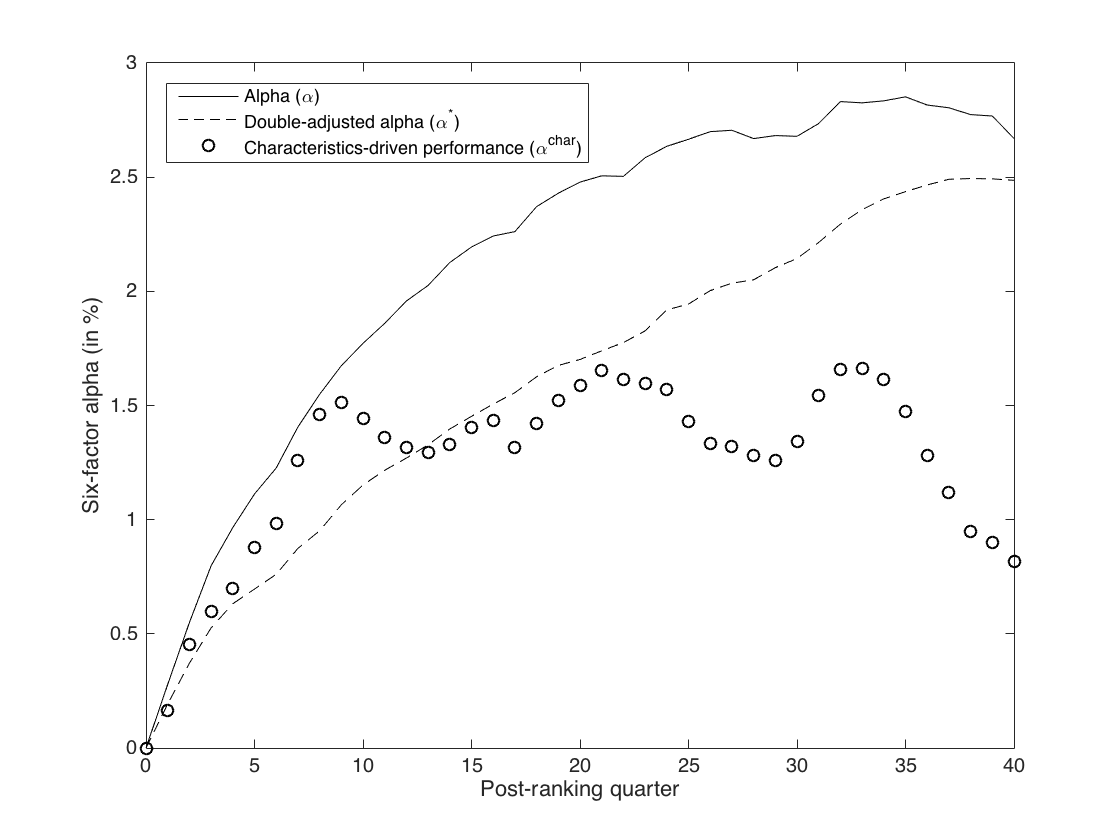
\includegraphics[width=14cm,height=7cm,\textwidth]{pictures/persistence.png}
%   {\captionsetup{justification=centering,singlelinecheck=off}
%   \caption{\bfseries Cumulative alphas for top-minus-bottom portfolios } } }  
% \caption*{This figure presents the cumulative post-ranking Fama-French six-factor alpha for top-minus-bottom portfolios sorted on one of the following performance measures: six-factor alpha ($\alpha$), double-adjusted six-factor alpha ($\alpha^*$), or characteristic-driven performance ($\alpha^{char}$). These performance measures are calculated using rolling windows with a window size of 24 months (see section \ref{double_alpha}). Portfolios are rebalanced every quarter-end and held up to 40 quarters. The horizontal axis shows the post-ranking holding period in quarters.}
% \end{figure}
% \end{singlespacing}


\subsection{Mutual Fund's R-squared}
 Recent studies show that fund performance is positively affected by fund selectivity or active fund management, which is measured by the deviation of fund holdings from a diversified benchmark portfolio. This selectivity measure requires data on the holdings of funds and knowledge on the benchmark indices of funds, which are difficult to obtain. In addition, the benchmark portfolio is not always accurately defined. \citet{amihud2013mutual} propose a simple and intuitive measure of mutual fund selectivity:\footnote{\citet{amihud2013mutual} define fund selectivity as 1 - $R^2$ = $\frac{\text{RMSE}^2}{\text{TotalVariance}}$ = $\frac{\text{RMSE}^2}{\text{SystemeticRisk}+\text{RMSE}^2}$. \newline RMSE is the idiosyncratic volatility, which is the volatility of the factor model residuals. SystemeticRisk is the return variance that is due to the risk factors. Fund selectivity is greater if the fund's idiosyncratic volatility is higher relative to its total variance, meaning that the fund's volatility is less driven by factor-based (systematic) volatility.  } the fund's R-squared ($R^2$), the proportion of the return variance that is explained by the benchmark portfolios, estimated from a multi-factor model. \citet{amihud2013mutual} hypothesize that a low $R^2$ corresponds to high stock selectivity, as a low $R^2$ indicates that mutual returns are not well explained by the Fama-French risk factors. In this respect, they find that $R^2$ has a negative and significant predictive effect on fund performance. 
We replicate the work of \citet{amihud2013mutual} by examining the relation between a fund's factor model $R^2$ and fund performance. Each month, we calculate a fund's $R^2$ from a six-factor model over a 24-month estimation period using daily returns. Following \citet{amihud2013mutual}, since the distribution of $R^2$ is negatively skewed, we apply the log transformation of $R^2$: $\tilde{R}^2$ = $\text{log}\left[\frac{\sqrt{R^2}}{(1-\sqrt{R^2})}\right]$. We test whether fund selectivity explains fund performance by the following panel regression
\begin{alignat}{2}
     \label{R2}
     \text{Performance}_{it} = & \hspace{0.1cm} c_{0t} + c_{1t}\tilde{R}^2_{it} + c_{2t}\text{ExpRatio}_{it-1} + c_{3t}\text{Turnover}_{it-1} + c_{4t}\text{log}(\text{TNA})_{it-1} \nonumber \\ 
     &+ c_{5t}
    \text{log}(\text{FundAge})_{it-1} + v_{it},
 \end{alignat}
 where $\text{Performance}_{it}$ refers to fund i's six-factor alpha ($\alpha$), double-adjusted six-factor alpha $(\alpha^{*}$),
or characteristic-driven performance ($\alpha^{char}$), all estimated over a rolling window of 24 months ending in month $t$. We relate fund performance to the contemporaneous log-transformed R-squared, $\tilde{R}^2$, which is measured over the same rolling window period. Lagged control variables are included in the regression comprising $\text{ExpRatio}$, the total expenses divided by a fund's Total Net Assets (TNA); $\text{Turnover}$, defined as the minimum of aggregated sales or aggregated purchases divided by TNA; $\text{TNA}$ in logarithm; and $\text{FundAge}$ in logarithm, computed as the difference in years between the current date and the date the fund was first offered. The model residuals are given by $v_{it}$. We estimate this regression in each month in our sample.
\par Table \ref{table7} reports the averaged cross-sectional regression coefficients along with Fama-MacBeth t-statistics with the \citet{newey1986simple} correction for time series correlation with 12 lags. Firstly, similar to the findings of \citet{amihud2013mutual}, we find that alpha is higher for funds with lower R-squared, that is, funds with high stock selectivity. The control variables yield no significant estimates. When we consider double-adjusted alpha we find no significant relation with $\tilde{R}^2$. However, the results indicate a significant (inverse) relation between the characteristic-driven component of alpha and R-squared, with t-statistics well above two. A potential reason might be that characteristics can help explain fund returns in cases where the Fama-French factors fail to do so, such that we find a strong inverse relation between characteristic-driven performance and R-squared. Thus, we find that inverse relation between alpha and R-squared does not indicate a positive relation between fund performance and fund selectivity, but rather indicates the poor explanatory power of the Fama-French style factor models. This calls into question the use of R-squared as a measure of fund selectivity. 

% \begin{singlespacing}
% \begin{table}[h!]
% \centering
% \small
% \setlength{\tabcolsep}{11pt}
% {\captionsetup{justification=centering,singlelinecheck=off}
% \caption{ \bfseries Relation between mutual fund performance and $R^2$ }}
% \caption*{This table presents the time series averages of monthly cross-sectional regressions of mutual fund performance measures on fund selectivity, measured by the contemporaneous log-transformed R-squared ($\tilde{R}^2$). As (annualized) performance measures we employ six-factor alpha ($\alpha$), double-adjusted six-factor alpha ($\alpha^*$) and characteristic-driven performance ($\alpha^{char}$). These performance measures are calculated using rolling windows with a window size of 24 months (see section \ref{double_alpha}). We estimate the regressions with and without a set of control variables. \citet{fama1973risk} t-statistics with the \citet{newey1986simple} correction of 12 lags are reported in parenthesis. Estimates significant at the 5\% are in bold font. The monthly regressions cover the period February 2001 until December 2016. }
% \label{my-label}
% \begin{tabular}{crrrrrrrr}
% \hline
%             & \multicolumn{2}{c}{$\alpha$} & &  \multicolumn{2}{c}{$\alpha^*$} &  & \multicolumn{2}{c}{$\alpha^{char}$} \\ \hline
% Cnst        & \textbf{4.770}           & \textbf{4.778}           &  & \textbf{-0.518}           & \textbf{-0.540}          &  & \textbf{1.073}            & \textbf{1.110}            \\
%             & (2.01)          & (1.98)          &  & (-2.12)                   & (-2.20)                  &  & (2.76)                    & (2.61)                    \\
% $\tilde{R}2$         & \textbf{-1.148} & \textbf{-1.269} &  & -0.018                    & -0.021                   &  & \textbf{-0.314}           & \textbf{-0.306}           \\
%             & (-2.12)         & (-2.36)         &  & (-1.02)                   & (-1.18)                  &  & (-2.67)                   & (-2.55)                   \\
% ExpRatio    &                 & 8.112           &  &                           & 0.848                    &  &                           & -0.548                    \\
%             &                 & (1.30)          &  &                           & (1.62)                   &  &                           & (-0.37)                   \\
% Turnover    &                 & -0.081          &  &                           & 0.001                    &  &                           & -0.002                    \\
%             &                 & (-1.78)         &  &                           & (0.32)                   &  &                           & (-0.29)                   \\
% Log(TNA)     &                 & -0.014          &  &                           & -0.001                   &  &                           & -0.002                    \\
%             &                 & (-1.07)         &  &                           & (-0.23)                  &  &                           & (-0.45)                   \\
% Log(FundAge) &                 & 0.015           &  &                           & 0.006                    &  &                           & -0.010                    \\
%             &                 & (0.48)          &  &                           & (1.45)                   &  &                           & (-0.60)                   \\ \hline
% \end{tabular}
% \end{table}
% \end{singlespacing}
%  \subsection{Mutual fund's deviation from benchmarks}
% \citet{jiang2014information} is another study which analyses the relation between fund selectivity and fund performance. They measure fund selectivity by computing the deviations of the weights of stocks in a fund's portfolio from those of the fund's benchmark portfolio. A fund's benchmark is determined by comparing the holdings of a fund with the holdings of most commonly used benchmarks and select the one for which the difference between weights are minimized. They indeed find that funds which deviate from benchmarks generate higher alphas than their low-deviation counterparts. 

\subsection{Mutual Fund Flows}
 There is no shortage of literature on mutual fund flows. The first stream of literature (e.g., \citet{warther1995aggregate}, \citet{edelen2001aggregate}, \citet{brown2003investor}) have focused on aggregate fund flows to the equity market, documenting a positive correlation with contemporaneous stock returns. Early works of \citet{ippolito1992consumer}, \citet{gruber1996another} and \citet{sirri1998costly} find that capital flows to and from funds are strongly related to past fund performance. The general consensus is that the flow-performance relation is positive, asymmetric and convex; the inflows generated by positive returns is of greater magnitude than the outflows due to negative returns. The establishment of a convex flow-performance relation is generally robust to different performance measures varying from raw returns to multi-factor model alphas.
 
 More recently, a second stream of literature goes beyond the simple flow-performance relations.\footnote{A mutual fund's investment style is an important source of information to investors. \citet{cooper2005changing} document an increase in fund flows to funds adopting the current hot investment style in their names. They find that these inflows are similar across funds who alter their positions matching their new name and those who do not, suggesting that investors are irrationally influenced by cosmetic effects. \citet{guo2016mutual} use a fund's reported holdings to determine a fund's investment style and find that funds adopting a more volatile implementation of style strategy garner higher inflows.} A recent paper of \citet{barber2016factors} investigate which risk factors are used by investors to adjust raw returns when evaluating fund performance. They run linear regressions of fund flows on fund alphas obtained from several Fama-French factor models and conclude that CAPM alphas are the best predictor of flows among all factor model alphas. In additional analysis, they decompose fund returns into alpha and returns resulting from factor tilts. They conclude that alpha generates the largest flow response, closely followed by a fund's momentum related return, while flows are least sensitive to fund returns traced to market beta. 
 
We aim to replicate the work of \citet{barber2016factors} using our decomposition of traditional alpha. Using fund flows, we investigate whether investors tend toward the double-adjusted component $\alpha^*$ or toward the characteristic-driven component $\alpha^{char}$ when assessing fund managers. For this purpose, we follow the majority of the prior literature on fund flows and calculate net capital flow\footnote{\citet{frazzini2008dumb} and \citet{lou2012flow} correct for fund mergers when calculating fund flows. As fund mergers are quite rare, this study ignores them.} to fund $i$ during month $t$ as 
 
  \begin{equation}
\label{flow}
    \text{flow}_{it} = \frac{\text{TNA}_{it} - \text{TNA}_{it-1}  (1+R_{it})}{\text{TNA}_{it-1}},
\end{equation}
where $\text{TNA}_{it}$ is fund $i$'s total net assets at the end of month $t$ and $\text{R}_{it}$ is the monthly net return of fund $i$ in month $t$.\footnote{ Fund flows are dropped if the percentage difference in TNA in between two months is greater than 200\% or less than -50\%. These extreme flows are rare and are typically related to structural changes within funds, e.g., mergers.} The variable flow reflects the percentage growth of a fund that is due to new investment (under the assumption of dividends being reinvested in the fund).

% \subsubsection*{Pairwise comparison between performance measures}
% First, we are interested in testing whether the decision-making of fund investors are sensitive to double-adjusted alphas relative to alphas. We consider a pairwise comparison between alpha and double-adjusted alpha. To do so, we proceed as follows. Each month $t$, we sort funds into deciles using both performance measures estimated over the past 36 months. Decile 10 contains the best performing funds, and decile 1 contains the worst performing funds. Thus, we end up with a monthly time-series of two decile ranks (for both alpha and double-adjusted alpha) for each fund.  
% \par 
% We conduct the pairwise comparison by estimating the flow-performance relation with the following panel regression using OLS: 
% \begin{equation}
%     \label{flow_decile} 
%     \text{flow}_{it} = b_0+ \sum^{10}_{k=1} \sum^{10}_{l=1} b_{ab} D_{abit-1} + \gamma X_{it} + \epsilon_{it},
% \end{equation}
% where the dependent variable is the monthly fund flow of fund $i$ in month $t$.  $D_{abit-1}$ is a dummy variable which equals one if fund $i$ in month $t$-1 is in decile $a$ based on alpha and decile $b$ based on double-adjusted alpha. To avoid the dummy variable trap, we exclude the dummy variable for $a$ = 5 and $b$ = 5. The matrix $X_{it}$ contains fund-specific control variables, and $\gamma$ is a vector with corresponding coefficient estimates. The control variables include the previous month-end TNA and the mean of monthly flows over the past year. $\epsilon_{it}$ are the model residuals. The coefficients of interest are $b_{ij}$, which represent the percentage flow received by a fund in decile $a$ using alpha and decile $b$ using double-adjusted alpha. To account for time-fixed effects, we estimate this regression with monthly dummy variables. \par We compare the coefficients for which the decile ranks of both performance measures are equal, but in reversed order. For instance, we compare the coefficient estimate for the dummy variable with funds in the top decile for the alpha and the bottom decile for the double-adjusted alpha ($b_{10,1}$), with the coefficient estimate using funds in the bottom decile for alpha and the top decile for double-adjusted alpha ($b_{1,10}$). If investors favor alpha over double-adjusted alpha to assess fund performance, we expect $b_{10,1}$ $>$ $b_{1,10}$; conversely, if investors are more sensitive to double-adjusted alpha, we expect $b_{10,1}$ $<$ $b_{1,10}$. We conduct this head-to-head comparison for all decile rank combinations, totalling 45 comparisons of coefficients. We test the null hypothesis that the summed difference across all comparisons is equal to zero. Moreover, we compute a binomial test statistic to test the null hypothesis that the percentage of positive coefficient differences is equal to 50\%. 
% \par Figure 3 summarizes the results of the pairwise comparison between the performance measures. In the top left plot, we graph the 45 differences in coefficient estimates when we compare standard four-factor alpha to double-adjusted four-factor alpha as a predictor of fund flows. The horizontal axis displays the decile ranks of both performance measures which are compared. For instance, the bar with label "10v9" contains the difference between the coefficient for funds with alpha ranking of 10 and double-adjusted alpha rank of 9. Overall, funds with higher decile rankings using alpha garner more flows than using double-adjusted alpha. The sum of the differences between coefficients is 47 (t = 3.21), while 83\% of the differences are in favor of alpha. We repeat this procedure and compare the two components of alpha: double-adjusted alpha and characteristic-driven performance (see Eqs.(\ref{double_alpha})-(\ref{char})). The right plot in Figure 3 shows a consistent pattern of positive differences, which indicates that fund flows follow double-adjusted alpha rather than the characteristic-driven component. \par As expected, alpha carries more weight in the assessment of fund performance by investors. \citet{barber2016factors} find that CAPM alphas are the best predictor of flows in comparison to the known multi-factor models. In this light, we can not expect investors to perform a second adjustment to alphas when assessing fund performance.
% However, when we decompose alpha we find that double-adjusted alpha is the component which garners the most flows. That is, in aggregate, investors do not allocate capital to abnormal returns related to the characteristic component of alpha. 

\par Similar to \citet{barber2016factors}, we further decompose characteristic-driven performance into alpha related to each individual characteristic. Recall that characteristic-driven performance (see Eq.(\ref{char})) is defined as
\begin{alignat}{2}
\label{char_decomp}
 \alpha^{char}_{it} &= \delta'_{1t}Z_{it-1} \nonumber \\ 
 &= \delta^{\text{Mcap}}_{1t}\text{Mcap}_{it-1}  + \delta^{\text{B/M}}_{1t}\text{B/M}_{it-1} +  \delta^{\text{Mom12}}_{1t}\text{Mom12}_{it-1} + \delta^{\text{Profit}}_{1t}\text{Profit}_{it-1} + 
 \delta^{\text{Invest}}_{1t}\text{Invest}_{it-1} 
\end{alignat}
which is the sum of lagged (standardized) characteristics multiplied by the corresponding cross-sectional premia. With this decomposition, we gauge whether fund flows are distributed differently across the characteristic components of alpha by estimating the following panel regression 
\begin{alignat}{2}
    \label{decomp}
       \text{flow}_{i,t+1:t+12} = & \hspace{0.1cm} c_{0t} + c_{1t} \alpha^*_{it} + c_{2t} [\delta^{\text{Mcap}}_{1t}\text{Mcap}_{it-1}]  + c_{3t} [\delta^{\text{B/M}}_{1t}\text{B/M}_{it}] +  c_{4t}[\delta^{\text{Mom12}}_{1t}\text{Mom12}_{it-1}] \nonumber \\
        &+ c_{5t}[\delta^{\text{Profit}}_{1t}\text{Profit}_{it-1}] + 
 c_{6t}[\delta^{\text{Invest}}_{1t}\text{Invest}_{it-1}]  \nonumber \\ 
 &+ c_{7t}\text{ExpRatio}_{it} + c_{8t}\text{Turnover}_{it} + c_{9t}\text{log}(\text{TNA})_{it} + c_{10t}\text{log}(\text{FundAge})_{it} + v_{it},
\end{alignat}
where the dependent variable is the average monthly fund flow of fund $i$ in the following year. The independent variables include double-adjusted alpha $\alpha^*_{it}$ and alpha related to a fund's size, value, momentum, profitability and investment characteristics (see Eq.(\ref{char_decomp})). We include the same control variables as in Eq.(\ref{R2}). The model residuals are given by $v_{it}$. We estimate this regression at each year-end. We expect that managerial skill attracts fund, such that there is no capital directed towards abnormal return related to known characteristics. That is, we expect that the parameters related to the characteristic components to be indistinguishable from zero. Contrary evidence implies that either investors are not considering known factors when assessing fund performance, or alpha provides an incomplete risk-adjustment for these characteristics.

% \begin{singlespacing}
% \begin{table}[h!]
% \setlength{\tabcolsep}{23pt}
% \centering
% \small
% {\captionsetup{justification=centering,singlelinecheck=off}
% \caption{ \bfseries Response of fund flows to components of alpha }}
% \caption*{This table presents the time series averages of annual cross-sectional regressions of the one-year ahead average of monthly fund flows on double-adjusted six-factor alpha ($\alpha^*$) and characteristic-driven performance ($\alpha^{char}$). These performance measures are calculated using rolling windows with a window size of 24 months (see section \ref{double_alpha}). We also estimate the regressions in which we further decompose $\alpha^{char}$ into alpha related to each individual characteristic. We estimate the regressions with and without a set of control variables. \citet{fama1973risk} t-statistics with the \citet{newey1986simple} correction of 3 lags are reported in parenthesis. Estimates significant at the 5\% are in bold font. We estimate these annual regressions at the end of each year, covering 16 years from 2001 to 2016.}
% \label{my-label}
% \begin{tabular}{crrrr}
% \hline
% Cnst                    & \textbf{0.014} & 0.004          & \textbf{0.014}  & 0.005           \\
%                         & (6.69)         & (0.58)         & (6.48)          & (0.69)          \\
% $\alpha^*$                      & \textbf{4.061} & \textbf{4.044} & \textbf{4.065}  & \textbf{4.047}  \\
%                         & (9.75)         & (9.80)         & (9.75)          & (9.81)          \\
% $\alpha^{char} & \textbf{0.396} & \textbf{0.366} &                 &                 \\
%                         & (2.41)         & (2.16)         &                 &                 \\
% $\delta^{\text{Mcap}}$ $\cdot$ Mcap            &                &                & \textbf{-1.476} & \textbf{-1.455} \\
%                         &                &                & (-2.19)         & (-2.11)         \\
% $\delta^{\text{B/M}}$ $\cdot$ B/M              &                &                & 0.275           & 0.215           \\
%                         &                &                & (0.31)          & (0.24)          \\
% $\delta^{\text{Mom12}}$ $\cdot$ Mom12              &                &                & \textbf{1.778}  & \textbf{1.720}  \\
%                         &                &                & (3.06)          & (2.91)          \\
% $\delta^{\text{Profit}}$ $\cdot$ Profit           &                &                & 0.338           & 0.221           \\
%                         &                &                & (0.37)          & (0.22)          \\
% $\delta^{\text{Invest}}$ $\cdot$ Invest            &                &                & 1.776           & 1.694           \\
%                         &                &                & (0.85)          & (0.87)          \\
% ExpRatio                &                & 0.481          &                 & 0.468           \\
%                         &                & (1.42)         &                 & (1.40)          \\
% Turnover                &                & 0.000          &                 & 0.000           \\
%                         &                & (-0.96)        &                 & (-1.07)         \\
% Log(TNA)                 &                & 0.000          &                 & 0.000           \\
%                         &                & (-0.82)        &                 & (-0.82)         \\
% Log(FundAge)             &                & 0.002          &                 & 0.002           \\
%                         &                & (1.75)         &                 & (1.78)          \\ \hline
% \end{tabular}
% \end{table}
% \end{singlespacing}

% \vspace{-0.45cm}
\par 
Table \ref{table8} reports the cross-sectional regression coefficients averaged across time along with Fama-MacBeth t-statistics with the \citet{newey1986simple} correction for time series correlation with 3 lags. In the first two columns, we specify future fund flows as a linear combination of double-adjusted alpha and characteristic-driven performance, with and without the set of control variables. We find strong positive relations between both performance measures and fund flows, where the double-adjusted component garners the most inflows. Among the set of control variables, we find positive but statistically insignificant coefficients for $\text{ExpRatio}$ and $\text{log}(\text{FundAge})$.
Of interest are the estimated sensitivities of flows to the characteristic components of alpha. Generally, fund returns related to characteristics do not garner the same magnitude of flows as double-adjusted alpha does. The coefficients on the value and profitability characteristics are both statistically and economically insignificant. However, we do find evidence of investors tending to size and momentum characteristics, which yield significant parameter estimates of about half of that of double-adjusted alpha (in absolute value).  Thus, in aggregate, we find that the flow-performance relation is mostly driven by double-adjusted alpha and that investors allocate a portion of their investment toward funds with favourable characteristics in the size and momentum dimensions. 
\par In sum, we have replicated parts of the analysis from several papers on mutual fund performance. First, we find stronger evidence of return persistence when using double-adjusted alpha. Second, we find that the inverse relation between alpha and R-squared is mostly driven by the characteristic-component of alpha. Third, fund flows are more responsive to double-adjusted alpha rather than characteristic-driven performance. These findings show that adjusting alphas for characteristics materially impacts previous findings on mutual fund performance. As our results together with those of \citet{busse2017double} indicate that double-adjusted alpha better reflects true skill, we believe that this performance measure should be used to reassess previous studies and in future studies on mutual fund performance. 

\section{Robustness Checks}
 \subsection{Overlapping Rolling Windows}
In a recent paper, \citet{britten2011improved} examine the impact of overlapping dependent variables on the inference from standard Fama-MacBeth cross-sectional regressions. The overlap induces an autocorrelation pattern in the standard errors of the cross-sectional regressions and commonly used methods (e.g., White or common Newey-West standard errors) to deal with this autocorrelation are inadequate and can lead to misleading estimates of the confidence intervals associated with coefficient estimates obtained from finite samples.\footnote{\citet{britten2011improved} transform original regressions into an equivalent representation in which the dependent variables are non-overlapping to remove the autocorrelation. Their method is easily applicable within standard frequentist analyses and they show that conventional inference procedures (OLS-, White-, Newey-West- standard errors) are asymptotically valid when applied to the transformed regression.} As the rolling windows overlap in our model in Eqs.(\ref{asset}), (\ref{cross}) and (\ref{delta_t}), we check the robustness of our results in Section \ref{estimation_results}.  Specifically, we re-estimate our model using different frequencies of the cross-sectional regressions in Eq.(\ref{cross}).
\par Table \ref{table9} reports the results. In Panel A, we estimate the cross-sectional regressions at each quarter-end rolling the window three months at a time. The results are very similar compared to the results using monthly cross-sectional regressions (see Table \ref{table3}).\footnote{We repeated the analysis of Section \ref{relative_performance} using double-adjusted alpha obtained from quarterly cross-sectional regressions. In untabulated results, we find that inference is qualitatively similar to that based on double-adjusted alpha from monthly cross-sectional regressions.} All characteristics except operating profitability remain significantly associated with six-factor alphas. Moreover, we find an increase in the posterior standard deviations for the momentum, profitability and investment characteristics. In Panel B, we estimate the cross-sectional regressions at a semi-annual frequency. We use less periods to estimate the systematic relation between alphas and characteristics, which leads to a further increase in posterior standard deviations. Consequently, we find more tenuous relations between six-factor alphas and the momentum and investment characteristics.
\par Another factor to consider is the frequency of mutual fund portfolio disclosure. The Thomson Reuters database provides quarterly snapshots of fund portfolios, which we keep constant between quarters to create a monthly time series of fund holdings (see Appendix A). Consequently, the variation in fund-level characteristics within quarters is only caused by the monthly variation in firm characteristics of each fund position. The staleness in our holdings data might compound the autocorrelation in the standard errors described above. While our analysis would benefit from portfolio disclosure at a higher frequency, the potential effects of frequent mutual fund portfolio disclosure remains the focus of a longstanding debate among practitioners, regulators, and academics.

% \begin{singlespacing}
% \begin{table}[h!]
% \small
% \centering
% \setlength{\tabcolsep}{16.5pt}
% {\captionsetup{justification=centering,singlelinecheck=off}
% \caption{\bfseries Rolling window frequency robustness}}
% \caption*{This table presents the results of the estimation of the model in Eqs.(\ref{asset}), (\ref{cross}) and (\ref{delta_t}) using different frequencies of the cross-sectional regressions in Eq.(\ref{cross}). We estimate this model during the period February 2001 to December 2016, using an estimation period of two years to estimate the six-factor model in Eq.(\ref{asset}), rolling the window three months at a time between quarter-ends in Panel A and six months at a time in Panel B. The characteristics (Z) are the logarithm of market capitalization (Mcap), the logarithm of book-to-market ratio (B/M), the logarithm of one plus the past twelve-month cumulative return (Mom12), operating profitability (Profit) and asset growth (Invest). Each characteristic is standardized by subtracting the cross-sectional mean each month. We estimate the model for each characteristic in isolation and for all characteristics in a joint model. We presents the posterior mean and standard deviation for the aggregate-level parameters in $\bar{\delta}$, based on the posterior distribution of the parameters constructed from 5000 iterations of the Gibbs sampler with the first 2500 iterations discarded as a burn-in period. Estimates in bold font indicate that the 95\% credible interval of the posterior distribution does not include zero. 
% }
% {\captionsetup{justification=centering,singlelinecheck=off}

% \begin{tabular}{crrrrrr}
% \hline
% \multicolumn{7}{l}{Panel A:  Quarterly cross-sectional regressions}                                                                                                                          \\
% Cnst   & \textbf{-0.003}      & \textbf{-0.003}      & \textbf{-0.003}      & \textbf{-0.003}             & \textbf{-0.003}                    & \textbf{-0.002}             \\
%       & (0.000)              & (0.000)              & (0.000)              & (0.000)                     & (0.000)                            & (0.000)                     \\
% Mcap   & \textbf{-0.002}      &                      &                      &                             &                                    & \textbf{-0.002}             \\
%       & (0.000)              &                      &                      &                             &                                    & (0.000)                     \\
% B/M    &                      & \textbf{-0.003}      &                      &                             &                                    & \textbf{-0.004}             \\
%       &                      & (0.000)              &                      &                             &                                    & (0.001)                     \\
% Mom12  &                      &                      & \textbf{0.019}       &                             &                                    & \textbf{0.005}                       \\
%       &                      &                      & (0.003)              &                             &                                    & (0.005)                     \\
% Profit &                      &                      &                      & -0.011                      &                                    & -0.003                      \\
%       &                      &                      &                      & (0.003)                     &                                    & (0.002)                     \\
% Invest &                      &                      &                      &                             & \textbf{0.022}                     & \textbf{0.016}              \\
%       &                      &                      &                      &                             & (0.007)                            & (0.007)                     \\
%       &                      &                      &                      &                             &                                    &                             \\
% \multicolumn{7}{l}{Panel B:  Semi-annual cross-sectional regressions}                                                                                                                        \\
% Cnst                 & \textbf{-0.003} & \textbf{-0.003} & \textbf{-0.003} & \textbf{-0.003} & \textbf{-0.003} & \textbf{-0.003} \\
%                      & (0.000)         & (0.000)         & (0.000)         & (0.000)         & (0.000)         & (0.000)         \\
% Mcap                 & \textbf{-0.002} &                 &                 &                 &                 & \textbf{-0.002} \\
%                      & (0.000)         &                 &                 &                 &                 & (0.000)         \\
% B/M                  &                 & \textbf{-0.003} &                 &                 &                 & \textbf{-0.003} \\
%                      &                 & (0.001)         &                 &                 &                 & (0.001)         \\
% Mom12                &                 &                 & \textbf{0.017}  &                 &                 & 0.006           \\
%                      &                 &                 & (0.004)         &                 &                 & (0.007)         \\
% Profit               &                 &                 &                 & -0.011          &                 & -0.003          \\
%                      &                 &                 &                 & (0.004)         &                 & (0.002)         \\
% Invest               &                 &                 &                 &                 & \textbf{0.017}  & 0.012           \\
%  &                 &                 &                 &                 & (0.009)         & (0.009)         \\ \hline
% \end{tabular}
% \end{table}
% \end{singlespacing}

\subsection{Characteristic-based Benchmark Approach}
\label{section5B}
\citet{daniel1997measuring} develop a new measure of mutual fund performance which use benchmarks based on the firm characteristics of mutual fund holdings. The benchmarks are constructed from the returns of passive portfolios sorted on characteristics that are matched with the characteristics of the evaluated fund's holdings. Specifically, the DGTW characteristic selectivity (CS) measure is calculated as 
\begin{equation}
    CS_{it} = \sum_{j=1}^{N_{it}} w_{jt-1} (R_{jt}-R^{b_{jt}}_t),
\end{equation}
where $w_{jt-1}$ is the portfolio weight on stock $j$ at the end of month $t-1$, $R_{jt}$ is the month $t$ return of stock $j$, $R^{b_{jt}}_t$ is the month $t$ return of the characteristic-based benchmark portfolio that is matched to stock $j$, and $N_{it}$ is the number of holdings of fund $i$ in month $t$. We use the DGTW CS measure to adjust fund returns for size, value, momentum, profitability and investment effects. In Appendix E, we describe the construction of the characteristic-based benchmark portfolios in greater detail. 
\par To test whether this characteristic-based performance measure fully adjusts fund returns for the main anomalies, we regress cross-sectionally the DGTW CS measure on the factor betas from the Fama-French six-factor model. Particularly, we conduct the following panel regression
\begin{equation}
    CS_{i,t-23:t} = c_{0t} + \sum^6_{k=1} c_{kt}\beta_{ikt} + v_{it},
\end{equation}
where the dependent variable is the average DGTW CS measure of fund $i$ across a 24-month period ending in month $t$. The independent variables include the six-factor betas of fund $i$ estimated over the same 24-month period using daily fund returns. The model residuals are given by $v_{it}$. Beginning with the $24^{\text{th}}$ month of our sample, we estimate the monthly cross-sectional regressions over the period December 2002 to December 2016, consisting of 169 months.
\par Table \ref{table10} reports the results. In Panel A, we only adjust returns for size, value and momentum effects. When considered in isolation, we find significant relations between the DGTW CS measure and the market, momentum and profitability betas. That is, the characteristic-based measure under-adjusts for exposures to the momentum and profitability factors. When we consider all factor betas together, the profitability beta is no longer significantly related with characteristic-adjusted fund performance. In Panel B, we adjust returns for all characteristics and the results are qualitatively similar. 
\par In sum, we conclude that the characteristic-based measure of \citet{daniel1997measuring} does not fully adjust fund performance for the main anomalies. Controlling only for factor betas, as in Fama-French factor models, or only for characteristics, as in DGTW, may overlook the other effect, and in so doing materially impact estimates of fund manager skill. 

% \begin{singlespacing}
% \begin{table}[h!]
% \setlength{\tabcolsep}{23pt}
% \centering
% \small
% {\captionsetup{justification=centering,singlelinecheck=off}
% \caption{ \bfseries DGTW CS measure vs. six-factor betas}}
% \caption*{This table presents the time series averages of monthly cross-sectional regressions of the DGTW characteristic selectivity (CS) measure on the Fama-French six-factor betas. We calculate the average DGTW CS measure across the past 24 months. We estimate the six-factor model over the same 24-month period using daily fund returns. In Panel A, the DGTW CS measure controls for the size, value and momentum characteristics. In Panel B, the DGTW CS measure also controls for the profitability and investment characteristics. \citet{fama1973risk} t-statistics with the \citet{newey1986simple} correction of 12 lags are reported in parenthesis. Estimates significant at the 5\% are in bold font. Starting with the $24^{\text{th}}$ month in our sample, the monthly regressions cover the period December 2002 to December 2016.}
% \setlength{\tabcolsep}{14pt}
% \label{my-label}
% \begin{tabular}{crrrrrrr}
% \hline
% \multicolumn{8}{l}{Panel A: Size, value and momentum characteristics}                                                     \\
% Cnst & \textbf{0.225}  & 0.003   & 0.001  & -0.004         & 0.013          & 0.003  & \textbf{0.207}  \\
%      & (3.30)          & (0.31)  & (0.06) & (-0.40)        & (1.81)         & (0.32) & (2.89)          \\
% RMRF & \textbf{-0.227} &         &        &                &                &        & \textbf{-0.211} \\
%      & (-3.09)         &         &        &                &                &        & (-2.71)         \\
% SMB  &                 & -0.008  &        &                &                &        & -0.008          \\
%      &                 & (-0.35) &        &                &                &        & (-0.31)         \\
% HML  &                 &         & 0.090  &                &                &        & 0.071           \\
%      &                 &         & (1.67) &                &                &        & (1.65)          \\
% WML  &                 &         &        & \textbf{0.207} &                &        & \textbf{0.323}  \\
%      &                 &         &        & (2.31)         &                &        & (3.89)          \\
% RMW  &                 &         &        &                & \textbf{0.116} &        & 0.063           \\
%      &                 &         &        &                & (2.03)         &        & (1.18)          \\
% CMA  &                 &         &        &                &                & 0.010  & 0.001           \\
%      &                 &         &        &                &                & (0.11) & (0.02)          \\
%      &                 &         &        &                &                &        &                 \\
% \multicolumn{8}{l}{Panel B: All characteristics}                                                      \\
% Cnst & \textbf{0.250}  & 0.006   & 0.007  & 0.000          & 0.016          & 0.011  & \textbf{0.218}  \\
%      & (3.54)          & (0.59)  & (0.68) & (0.01)         & (1.79)         & (1.20) & (3.31)          \\
% RMRF & \textbf{-0.246} &         &        &                &                &        & \textbf{-0.223} \\
%      & (-3.10)         &         &        &                &                &        & (-3.08)         \\
% SMB  &                 & 0.014   &        &                &                &        & 0.013           \\
%      &                 & (0.76)  &        &                &                &        & (0.60)          \\
% HML  &                 &         & 0.046  &                &                &        & 0.024           \\
%      &                 &         & (1.06) &                &                &        & (0.48)          \\
% WML  &                 &         &        & \textbf{0.237} &                &        & \textbf{0.351}  \\
%      &                 &         &        & (2.59)         &                &        & (4.11)          \\
% RMW  &                 &         &        &                & \textbf{0.092} &        & 0.067           \\
%      &                 &         &        &                & (2.23)         &        & (1.27)          \\
% CMA  &                 &         &        &                &                & 0.019  & 0.041           \\
%      &                 &         &        &                &                & (0.29) & (0.91)          \\ \hline
% \end{tabular}
% \end{table}
% \end{singlespacing} 

\section{Conclusion}
We propose a new approach to evaluate the performance of mutual funds. It combines traditional factor models as in \citet{carhart1997persistence,fama1993common} with the effects of firm and asset characteristics, conform the recent insight that these information sources complement each other in explaining asset returns \citep{avramov2006asset,brennan1998alternative,chordia2015cross}. \citet{busse2017double} shows that the firm and asset characteristics resulting from mutual fund holdings should also be included in analyses of mutual fund performance.    

Our approach consists of a hierarchical Bayesian model with three layers in the style of \citet{cederburg2015asset}. The first layer specifies a factor model for daily returns, whereas the second splits the intercept in the effect of firm and asset characteristics, and the remainder which we call the double-adjusted alpha. The third layer adds monthly time variation to it. The double-adjusted alpha for each asset and each point in time can be split in an aggregate time-random effect and a time- and asset-specific component. Though our model combines the same information as \citet{busse2017double} to construct the double-adjusted alpha, the Bayesian approach offers a couple of advantages. Whereas \citet{busse2017double} uses a two-pass estimation, our Bayesian approach estimates the time series and cross-sectional parts of the model in one pass which leads to efficiency gains and  automatically accounts for the estimation uncertainty that otherwise should be included in the second part. More generally, the posterior mean of the time-random component of alpha shows to which extent the aggregate mutual fund can deliver outperformance, while the prior can be used to specify the belief in outperformance. 

We apply our approach to analyse the performance of U.S. mutual funds over the period 2001--2016, with the risk factors from \citet{FAMA20151} and a momentum factor, as well as the corresponding characteristics. We show that both factor exposures and the effect of characteristics are needed to explain mutual fund performance, and that our Bayesian approach leads to more precise estimates than the frequentist approach. Moreover, we show that the ranking of mutual funds based on the posterior mean of the double-adjusted alpha differs substantially from the ranking that results from the traditional alphas based on factor models.

We then show how our new inferences on mutual fund performance impact research into the skill of mutual funds. Replacing the traditional alpha by our double-adjusted one leads to stronger evidence for persistence in the performance of mutual funds. However, when we use the double-adjusted alpha, we do not find a relation with the time-series $R^2$ of the factor regression anymore as in \citet{amihud2013mutual}, indicating that the $R^2$ cannot be interpreted as a measure of selectivity related to skill. We extend \citet{barber2016factors} by showing that fund flows are most responsive to the double-adjusted alpha, and not so much to the part that is related to characteristics. We interpret this as evidence that at least part of the investment community also adjusts returns for the part that can be explained by well-known return drivers.

Our findings contribute to the literature in two ways. First, we show how to efficiently estimate a double-adjusted alpha in a single-pass using Bayesian techniques. We argue theoretically and show empirically that our approach improves upon the more standard two-pass estimation methodology by offering better and more precise estimates. Second, we show that these improved inferences are relevant for studies related to the performance and skill of mutual funds. Some of the results from earlier studies turn out to be stronger, while other results vanish. Taken together, it means that we have to be careful in the investigation of mutual fund performance, and should make sure that we include the necessary information in the right way. Our paper shows how a straightforward Bayesian model can accomplish that.

\begin{comment}
\subsection{recent}
Growing concerns arise among academics and practitioners alike regarding the portfolio-based approach for identifying anomalies and, more generally, for testing asset-pricing models. This approach sorts stocks on a firm characteristic and constructs a zero-cost hedge portfolio which reflects the return differential between stocks in the top characteristic decile and stocks in the bottom characteristic decile. \citet{ang2008using} and \citet{fama2008dissecting}, among many others, argue that grouping stocks into portfolios and aggregating returns wastes and potentially distorts cross-sectional patterns in stock returns. Consequently, the Fama-French multi-factor models, that incorporate these portfolios as risk factors, do not fully adjust returns for the main anomalies. Instead of estimated factor betas many studies (e.g., \citet{avramov2006asset}, \citet{chordia2015cross}) have opted for individual firm characteristics to explain expected returns.
\par Our paper moves the debate of factor betas versus characteristics to the returns of mutual funds. Specifically, we incorporate both in the performance evaluation of mutual funds by constructing a performance measure that adjusts returns for both factor betas and characteristics simultaneously. While it is debatable whether fund managers that actively shift their portfolios towards a certain characteristic dimension qualifies as skill, we believe that a performance measure should fully adjust for an anomaly. \citet{busse2017double} was the first to propose such a double-adjusted alpha which is calculated in a two-step procedure. We propose to estimate a double-adjusted alpha by a hierarchical Bayesian approach, which poses several advantages over the approach in \citet{busse2017double}. These advantages mainly stem from the simultaneous estimation of the performance measure, which circumvents using estimates of alpha in a second-pass regression. 
\par Similar to \citet{busse2017double}, we find that characteristics are statistically significantly related to fund returns even after controlling for factor model betas, suggesting that performance identified via Fama-French factor models could be attributed to loadings on characteristics. When we reassess several previous studies on mutual fund relative performance, we find that our double-adjusted performance measure is a purer measure of skill when we analyze persistence in fund performance. Moreover, we find that relations between specific fund features (fund selectivity and fund flows) and fund performance is partially driven by the characteristic component of performance. All in all, by more fully adjusting performance for the influence of characteristics we might alter previous inference on relative mutual fund performance. 
\par Our hierarchical Bayes model can be extended in various directions. For example, the MIDAS approach of \citet{ghysels2005there} can be adopted to assign optimal weights to the daily returns in the window used to estimate the rolling window factor betas. In addition, one can impose a common structure on the factor betas too, rather than just the alphas, to further exploit information from the cross-section of funds. Furthermore, while we focus on the characteristics underlying the Fama-French factors because of the widespread use of the Fama-French models, our model can be readily extended to adjust performance for other characteristics such as those underlying the q-factors from \citet{hou2015digesting} or underlying the short- and long-run behavioral factors from \citet{daniel2017short}. 

subsection{old}
Growing concerns arise among academics and practitioners alike regarding the portfolio-based approach for identifying anomalies and, more generally, for testing asset-pricing models. This approach sorts stocks on a firm characteristic and constructs a zero-cost hedge portfolio which reflects the return differential between stocks in the top characteristic decile and stocks in the bottom characteristic decile. \citet{ang2008using} and \citet{fama2008dissecting}, among many others, argue that grouping stocks into portfolios and aggregating returns wastes and potentially distorts cross-sectional patterns in stock returns. Consequently, the Fama-French multi-factor models, that incorporate these portfolios as risk factors, do not fully adjust returns for the main anomalies. Instead of estimated factor betas many studies (e.g., \citet{avramov2006asset}, \citet{chordia2015cross}) have opted for individual firm characteristics to explain expected returns.
\par Our paper moves the debate of factor betas versus characteristics to the returns of mutual funds. We conduct monthly cross-sectional regressions
of fund returns on estimated factor betas and firm-level characteristics (aggregated to a fund-level statistic from a fund's holdings). Similar to the evidence on stock returns, we find that factor betas and characteristics each account for about half of the total model explained variation in fund returns. Thus, despite the mechanical relation one might expect between factor betas and their underlying characteristics, our results imply they do not convey identical information.  
\par An important application of the Fama-French factor models is the performance evaluation of mutual funds. Since these factor models do not fully account for the main anomalies, they only partially control for passive influences on fund returns. Our paper proposes a new performance measure that adjusts fund returns for both factor exposures and characteristics simultaneously. While it is debatable whether fund managers that actively shift their portfolios towards a certain characteristic dimension qualifies as skill, we believe that a performance measure should fully adjust for a particular anomaly. 
\par To calculate our double-adjusted performance measure, we propose a hierarchical Bayes structure in which we simultaneously model conditional factor model alphas and analyze the cross-sectional relation between fund alphas and characteristics. We find that characteristics are statistically significantly related to fund returns even after controlling for factor model betas, suggesting that performance identified via Fama-French factor models could be attributable to loadings on characteristics. When we reassess several previous studies on mutual fund relative performance, we find that our double-adjusted performance measure is a purer measure of skill when we analyze persistence in fund performance. Moreover, we find that relations between specific fund features (fund selectivity and fund flows) and fund performance is partially driven by the characteristic component of performance. All in all, by more fully adjusting performance for the influence of characteristics we might alter previous inference on relative mutual fund performance. 
\par Our hierarchical Bayes model can be extended in various directions. For example, the MIDAS approach of \citet{ghysels2005there} can be adopted to assign optimal weights to the daily returns in the window used to estimate the rolling window factor betas. In addition, one can impose a common structure on the factor betas too, rather than just the alphas, to further exploit information from the cross-section of funds. Furthermore, while we focus on the characteristics underlying the Fama-French factors because of the widespread use of the Fama-French models, our model can be readily extended to adjust performance for other characteristics such as those underlying the q-factors from \citet{hou2015digesting} or underlying the short- and long-run behavioral factors from \citet{daniel2017short}. 
\end{comment}


\newpage 

 \bibliographystyle{apacite}
\bibliography{bronnen.bib}
\addcontentsline{toc}{section}{\protect\numberline{}References}%

\newpage
\begin{singlespacing}
\begin{figure}[H]
\centering
  \captionsetup{justification=left}
    {\captionsetup{justification=centering,singlelinecheck=off}
\caption{\bfseries Time series plots of the posterior means of the time-varying relation between six-factor alphas and characteristics $\delta_t$} \label{figure1} } 
\caption*{The figure presents estimation results of the model in Eqs.(\ref{asset}), (\ref{cross}) and (\ref{delta_t}) examining the cross-sectional relation between six-factor alphas and all characteristics simultaneously. In each plot we report posterior results for a given characteristic across our sample period February 2001 to December 2016. The solid line is the posterior mean of $\delta_t$ and the dashed lines represent the 95\% credible interval.}
  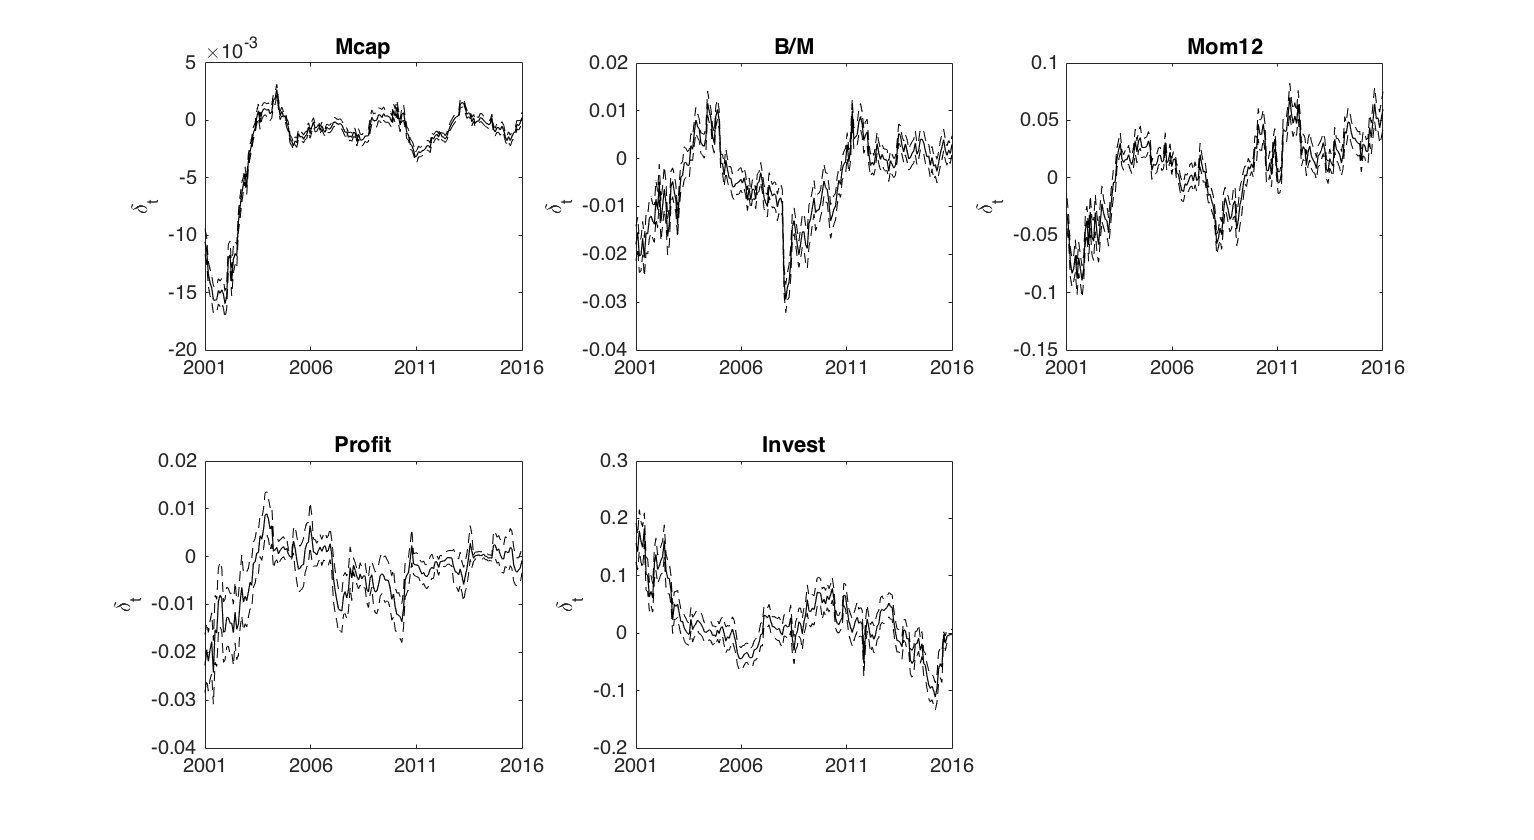
\includegraphics[width=18cm,height=10cm,\textwidth]{pictures/posterior_plots.png}

\end{figure}
\end{singlespacing}

\begin{singlespacing}
\begin{figure}[H]
\centering
  \captionsetup{justification=left}
  {\captionsetup{justification=centering,singlelinecheck=off}
  \caption{\bfseries Cumulative alphas for top-minus-bottom portfolios }\label{figure2} } 
\caption*{This figure presents the cumulative post-ranking Fama-French six-factor alpha for top-minus-bottom portfolios sorted on one of the following performance measures: six-factor alpha ($\alpha$), double-adjusted six-factor alpha ($\alpha^*$), or characteristic-driven performance ($\alpha^{char}$). These performance measures are calculated using rolling windows with a window size of 24 months. Portfolios are rebalanced every quarter-end and held up to 40 quarters. The horizontal axis shows the post-ranking holding period in quarters.}
  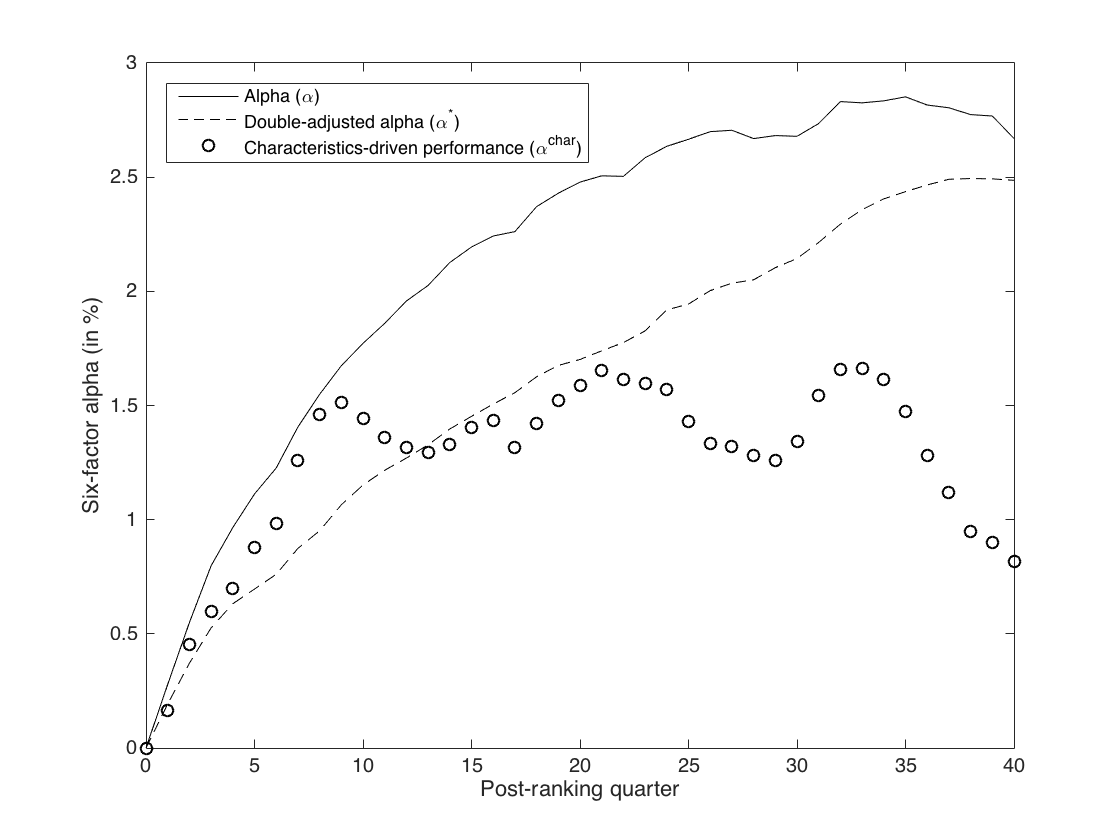
\includegraphics[width=14cm,height=7cm,\textwidth]{pictures/persistence.png}

\end{figure}
\end{singlespacing}

\begin{singlespacing}

\begin{table}[H]
\centering
\small
{\captionsetup{justification=centering,singlelinecheck=off}
\caption{\bfseries Summary statistics of equity mutual fund sample} \label{table1}}
\caption*{This table presents the summary statistics for the equity mutual funds sample over the period January 2001 to December 2016. Panel A reports statistics on the sample size. Panel B reports additional information on the funds. Panel C reports the cross-sectional distribution of characteristics averaged across all sample months. We weight each firm characteristic according to its current portfolio weight and calculate a fund's portfolio-weighted average characteristic. Market capitalization (Mcap) is the product between the previous month-end stock price and the previous month-end total shares outstanding. Book-to-Market (B/M) is the ratio between the most recently available book value of equity and the previous month-end market capitalization. Momentum (Mom12) is the past twelve-month cumulative return excluding the most recent month. Operating profitability (Profit) is the current revenues minus costs of goods sold, interest expense, selling, general, and administrative expenses, divided by book equity for the last fiscal year $t-1$.  Asset growth (Invest) is the percentage change in total assets from fiscal year $t-2$ to fiscal year $t-1$. Panel D reports the time series averages of the cross-sectional distributions of six-factor betas, which are estimated from rolling time series regressions using the past two years of daily fund returns. Panel E reports the time series averages of the cross-sectional correlations between factor betas and characteristics.}
\begin{tabular}{lrrrrr}
\hline
                                                & Mean     & \begin{tabular}[c]{@{}l@{}}25\%\\ percentile\end{tabular} & Median   & \begin{tabular}[c]{@{}l@{}}75\%\\ percentile\end{tabular} & \begin{tabular}[c]{@{}l@{}}Standard \\ deviation\end{tabular} \\ \hline
\multicolumn{6}{l}{Panel A: Observations}                                                                                                                               \\
Number of distinct funds                        & 2,871    &                                                         &          &                                                           &                                                               \\
Number of fund-report dates                     & 92,903  &                                                         &          &                                                           &                                                               \\
Number of fund-month dates                      & 314,362   &                                                         &          &                                                           &                                                               \\
Number of distinct stocks                       & 7,952    &                                                         &          &                                                           &                                                               \\
                                                &          &                                                         &          &                                                           &                                                               \\
\multicolumn{6}{l}{Panel B: Fund characteristics}                                                                                                                                                                                                           \\
Fund age                             & 22.90   & 15.76 & 19.96  & 25.38  & 12.33   \\
Fund monthly net return (in \%)      & 0.51    & -2.08 & 0.99   & 3.60   & 5.12    \\
TNA (total net assets) (in millions) & 1,341.43 & 56.00 & 220.00 & 863.10 & 5,335.74 \\
Expense ratio (in \%)                & 1.24    & 0.97  & 1.19   & 1.45   & 0.63    \\
Turnover ratio (in \%)               & 83.19   & 34.00 & 62.00  & 105.00 & 101.68                                                \\
                                                &          &                                                         &          &                                                           &                          


                                  \\
\multicolumn{6}{l}{Panel C: Fund holdings characteristics}                                                                                                                                                                                           \\
Mcap (in millions) & 44,475.74 & 3,792.98 & 43,016.63 & 78,966.25 & 39,731.13 \\
B/M                 & 0.46     & 0.32    & 0.44     & 0.56     & 0.16     \\
Mom12  (in \%)      & 17.12    & 9.15    & 14.89    & 22.86    & 12.13    \\
Profit              & 0.46     & 0.35    & 0.42     & 0.50     & 0.24     \\
Invest              & 0.09     & 0.07    & 0.09     & 0.12     & 0.04                                               \\

                                                &          &                                                         &          &      

                                                    &                                                               \\
\multicolumn{6}{l}{Panel D: Rolling window fund six-factor betas}                                                                                                                                                                                                           \\
$\beta_{MKT}$ & 0.98  & 0.94  & 0.99  & 1.03 & 0.10 \\
$\beta_{SMB}$ & 0.20  & -0.08 & 0.07  & 0.46 & 0.34 \\
$\beta_{HML}$ & 0.00  & -0.16 & 0.01  & 0.16 & 0.21 \\
$\beta_{WML}$ & 0.02  & -0.05 & 0.01  & 0.09 & 0.12 \\
$\beta_{RMW}$ & -0.06 & -0.17 & -0.02 & 0.09 & 0.21 \\
$\beta_{CMA}$ & -0.04 & -0.15 & -0.02 & 0.10 & 0.21 \\ \hline
\end{tabular}
\end{table}
\end{singlespacing}

 \begin{singlespacing}
 \begin{table}[H]
\centering
 {\captionsetup{justification=centering,singlelinecheck=off}
 \caption*{\bfseries Table 1 (Continued) }}
 \caption*{\centering \small{Panel E: Cross-correlations between six-factor betas and characteristics}}

 \small
\label{my-label}
\begin{tabular}{lrrrrrrrrrr}

       \hline
       & \text{$\beta_{SMB}$}  &\text{$\beta_{HML}$}   &\text{$\beta_{WML}$}   & \text{$\beta_{RMW}$}  & \text{$\beta_{CMA}$}   & Mcap   & B/M    & Mom12   & Profit & Invest \\ \hline
$\beta_{MKT}$   & 0.096 & -0.093 & 0.113  & -0.204 & -0.173 & -0.023 & -0.114 & 0.170  & -0.004 & 0.077  \\
$\beta_{SMB}$   &       & 0.095  & 0.043  & -0.142 & -0.075 & -0.816 & 0.110  & 0.283  & -0.255 & -0.064 \\
$\beta_{HML}$   &       &        & -0.315 & 0.610  & 0.328  & -0.042 & 0.746  & -0.236 & -0.079 & -0.452 \\
$\beta_{WML}$   &       &        &        & -0.231 & -0.270 & -0.054 & -0.469 & 0.568  & 0.103  & 0.191  \\
$\beta_{RMW}$   &       &        &        &        & 0.361  & 0.246  & 0.367  & -0.283 & 0.136  & -0.274 \\
$\beta_{CMA}$   &       &        &        &        &        & 0.049  & 0.354  & -0.215 & -0.004 & -0.470 \\
Mcap   &       &        &        &        &        &        & 0.049  & 0.354  & -0.215 & -0.004 \\
B/M    &       &        &        &        &        &        &        & -0.363 & -0.189 & -0.486 \\
Mom12   &       &        &        &        &        &        &        &        & -0.003 & 0.054  \\
Profit &       &        &        &        &        &        &        &        &        & 0.049  \\ \hline
\end{tabular}
\end{table}
\end{singlespacing}

\begin{singlespacing}
\begin{table}[H]
\setlength{\tabcolsep}{4.5pt}
\centering
 {\captionsetup{justification=centering,singlelinecheck=off}
\caption{\bfseries Cross-sectional regressions of mutual fund returns} \label{table2}}
\caption*{This table presents the time series averages of risk premia ($\gamma$) estimated using the cross-section of mutual fund (monthly) returns following the \citet{fama1973risk} procedure. The monthly regressions are of the form: 
\begin{equation*}
R_{t} = \gamma_{0t} + \gamma_{1t}\hat{B}_{t-1} + \gamma_{2t}Z_{t-1} + \xi_{t}, \hspace{0.2cm} t=1,...,T.
\end{equation*} We employ the CAPM, the \citet{fama1993common} three-factor model, the \citet{carhart1997persistence} four-factor model, the \citet{FAMA20151} five-factor model and a six-factor model combining all factors. Factor betas ($\hat{B}$) are estimated from rolling time series regressions using daily returns from the past two years. The characteristics (Z) are the logarithm of market capitalization (Mcap), the logarithm of book-to-market ratio (B/M), the logarithm of one plus the cumulative past twelve-month cumulative return (Mom12), operating profitability (Profit) and asset growth (Invest). Each characteristic is winsorized at the 0.5\% and the 99.5\% levels. To address the EIV bias, we employ the EIV-corrected estimator of \citet{chordia2015cross}. Risk premia (in percent per month) are fitted using OLS, both with EIV-correction and without. \citet{fama1973risk} t-statistics are reported in parenthesis. Estimates significant at the 5\% are in bold font. Risk premia are estimated over the period February 2001 until December 2016.}
 \small
\label{my-label}
\begin{tabular}{lrrrrrrrrrrrrrr}
\hline
      & \multicolumn{2}{c}{CAPM}        &           & \multicolumn{2}{c}{FF 3FM}      &           & \multicolumn{2}{c}{Carhart 4FM}  &           & \multicolumn{2}{c}{FF 5FM}       &           & \multicolumn{2}{c}{FF 6FM}       \\ \cline{2-3} \cline{5-6} \cline{8-9} \cline{11-12} \cline{14-15} 
      & OLS            & EIV            &           & OLS            & EIV            &           & OLS            & EIV             &           & OLS            & EIV             &           & OLS            & EIV             \\ \hline
Cnst  & \textbf{1.013} & \textbf{1.020} &           & 0.685          & 0.628          &           & \textbf{0.887} & \textbf{0.857} &  & \textbf{0.651} & 0.638          &  & \textbf{0.769}  & \textbf{0.759} \\
      & (2.46)         & (2.49)         &           & (1.88)         & (1.67)         &           & (2.61)         & (2.38)         &  & (2.00)         & (1.93)         &  & (2.47)          & (2.37)         \\
$\beta_{MKT}$  & -0.071         & -0.080         &           & -0.011         & -0.011         &           & -0.029         & -0.033         &  & 0.130          & 0.177          &  & 0.100           & 0.133          \\
      & (-0.24)        & (-0.26)        &           & (-0.04)        & (-0.03)        &           & (-0.09)        & (-0.10)        &  & (0.46)         & (0.61)         &  & (0.35)          & (0.46)         \\
$\beta_{SMB}$ &                &                &           & 0.098          & 0.120          &           & 0.049          & 0.061          &  & 0.099          & 0.099          &  & 0.074           & 0.073          \\
      &                &                &           & (0.62)         & (0.66)         &           & (0.30)         & (0.33)         &  & (0.66)         & (0.59)         &  & (0.48)          & (0.42)         \\
$\beta_{HML}$  &                &                &           & \textbf{0.347} & \textbf{0.373} & \textbf{} & \textbf{0.372} & \textbf{0.412} &  & 0.220          & 0.190          &  & 0.266           & 0.252          \\
      &                &                &           & (2.12)         & (2.09)         &           & (2.04)         & (1.99)         &  & (1.45)         & (1.07)         &  & (1.61)          & (1.30)         \\
$\beta_{WML}$  &                &                &           &                &                &           & 0.176         & 0.227          &  &                &                &  & 0.114           & 0.195          \\
      &                &                &           &                &                &           & (1.14)        & (1.19)         &  &                &                &  & (1.01)          & (1.13)         \\
$\beta_{RMW}$ &                &                &           &                &                &           &                &                &  & 0.190          & 0.224          &  & 0.225           & 0.271          \\
      &                &                &           &                &                &           &                &                &  & (1.17)         & (1.16)         &  & (1.29)          & (1.32)         \\
$\beta_{CMA}$  &                &                &           &                &                &           &                &                &  & 0.152          & 0.141          &  & 0.173           & 0.164          \\
      &                &                &           &                &                &           &                &                &  & (1.13)         & (0.90)         &  & (1.33)          & (1.09)         \\
Mcap  & -0.065         & -0.065         &           & -0.047         & -0.043         &           & -0.055         & -0.052         &  & -0.050         & -0.051         &  & \textbf{-0.054} & -0.054         \\
      & (-1.97)        & (-1.97)        &           & (-1.46)        & (-1.24)        &           & (-1.79)        & (-1.56)        &  & (-1.82)        & (-1.77)        &  & (-1.96)         & (-1.89)        \\
B/M   & 0.004          & 0.003          &           & -0.074         & -0.082         &           & 0.072          & -0.085         &  & -0.025         & -0.010         &  & -0.031          & -0.017         \\
      & (0.04)         & (0.03)         &           & (-0.98)        & (-1.08)        &           & (-1.08)        & (-1.26)        &  & (-0.36)        & (-0.07)        &  & (-0.50)         & (-0.27)        \\
Mom12 & \textbf{0.783} & \textbf{0.787} & \textbf{} & \textbf{0.863} & \textbf{0.859} &           & 0.478          & 0.446          &  & \textbf{0.794} & \textbf{0.774} &  & 0.513           & 0.524          \\
      & (2.11)         & (2.12)         &           & (2.34)         & (2.36)         &           & (1.78)         & (1.67)         &  & (2.17)         & (2.13)         &  & (1.85)          & (1.81)         \\
Profit    & 0.066          & 0.065          &           & 0.047          & 0.046          &           & 0.019          & 0.016          &  & 0.030          & 0.025          &  & 0.003           & 0.000          \\
      & (1.18)         & (1.17)         &           & (0.94)         & (0.94)         &           & (0.40)         & (0.34)         &  & (0.68)         & (0.59)         &  & (0.07)          & (0.02)         \\
Invest  & -0.573         & -0.560         &           & -0.389         & -0.371         &           & -0.391         & -0.355         &  & -0.279         & 0.257          &  & -0.230          & -0.222         \\
      & (-1.69)        & (-1.67)        &           & (-1.43)        & (-1.38)        &           & (-1.53)        & (-1.40)        &  & (-1.14)        & (-0.97)        &  & (-0.98)         & (-0.87)         \\ \hline
\end{tabular}
\end{table}
\end{singlespacing}


\begin{singlespacing}
\begin{table}[H]
\small
\centering
\setlength{\tabcolsep}{16.5pt}
{\captionsetup{justification=centering,singlelinecheck=off}
\caption{\bfseries Six-factor alpha vs. characteristics} \label{table3}}
\caption*{This table presents the results of the estimation of the model in Eqs.(\ref{asset}), (\ref{cross}) and (\ref{delta_t}). We estimate this model in each month during the period February 2001 to December 2016, using an estimation period of two years to estimate the six-factor model in Eq.(\ref{asset}), rolling the window a month at a time.
 The characteristics (Z) are the logarithm of market capitalization (Mcap), the logarithm of book-to-market ratio (B/M), the logarithm of one plus the past twelve-month cumulative return (Mom12), operating profitability (Profit) and asset growth (Invest). Each characteristic is standardized by subtracting the cross-sectional mean each month. We estimate the model for each characteristic in isolation and for all characteristics in a joint model. Panel A presents the posterior mean and standard deviation for the aggregate-level parameters in $\bar{\delta}$, based on the posterior distribution of the parameters constructed from 5000 iterations of the Gibbs sampler with the first 2500 iterations discarded as a burn-in period. Panel B presents \citet{fama1973risk} estimates
 and \citet{fama1973risk} t-statistics with the \citet{newey1986simple} correction of 12 lags. In Panel A, estimates in bold font indicate that the 95\% credible interval of the posterior distribution does not include zero. In Panel B,  estimates in bold font indicate significance at the 5\% level.
}
{\captionsetup{justification=centering,singlelinecheck=off}

\begin{tabular}{lrrrrrr}
\hline
\multicolumn{7}{l}{Panel A: Simultaneous Bayesian estimation}                                   \\ Cnst & -\textbf{0.003}  & -\textbf{0.003} & -\textbf{0.003}& -\textbf{0.003}&-\textbf{0.003} & -\textbf{0.002}\\ & (0.000) & (0.000) & (0.000) & (0.000) & (0.000) & (0.000) \\ 
Mcap   & -\textbf{0.002}  &                 &                &        &                & \textbf{-0.002}         \\
      & (0.000)  &                 &                &        &                & (0.000)          \\
B/M    &         & \textbf{-0.003} &                &        &                & \textbf{-0.004} \\
      &         & (0.000)          &                &        &                & (0.000)          \\
Mom12  &         &                 & \textbf{0.019} &        &                & \textbf{0.005}  \\
      &         &                 & (0.002)         &        &                & (0.003)          \\
Profit &         &                 &                & -0.011  &                & -0.003         \\
      &         &                 &                & (0.002) &                & (0.002)          \\
Invest &         &                 &                &        & \textbf{0.024} & \textbf{0.017}  \\
      &         &                 &                &        & (0.004)         & (0.004)          \\
      &         &                 &                &        &                &                 \\
\multicolumn{7}{l}{Panel B: Two-step OLS approach}                                   \\  Cnst & -0.002 & -0.002 &-0.002 & -0.002 & -0.002  & -0.002 \\ & (-1.40) & (-1.40) & (-1.40) & (-1.40) & (-1.40) & (-1.40) \\ 
Mcap   & -0.001 &         &        &         &        & -0.002  \\
      & (1.81) &         &        &         &        & (-1.60)  \\
B/M    &        & \textbf{-0.005}  &        &         &        & \textbf{-0.006}  \\
      &        & (-2.45) &        &         &        & (-2.29) \\
Mom12  &        &         & \textbf{0.016}  &         &        & 0.002   \\
      &        &         & (4.66) &         &        & (0.18)  \\
Profit &        &         &        & -0.011  &        & \textbf{-0.005}  \\
      &        &         &        & (-1.57) &        & (-2.27) \\
Invest &        &         &        &         & \textbf{0.040}  & 0.023   \\
      &        &         &        &         & (2.27) & (1.26)        \\ \hline
\end{tabular}
\end{table}
\end{singlespacing}    

 \begin{singlespacing}
 \begin{table}[H]
\small
\centering
\setlength{\tabcolsep}{16.5pt}
{\captionsetup{justification=centering,singlelinecheck=off}
\caption{\bfseries Multi-factor model alphas vs. characteristics} \label{table4}}
\caption*{This table presents the results of the estimation of the model in Eqs.(\ref{asset}), (\ref{cross}) and (\ref{delta_t}) based on several Fama-French models. We employ the CAPM, the \citet{fama1993common} three-factor model, the \citet{carhart1997persistence} four-factor model, the \citet{FAMA20151} five-factor model and a six-factor model combining all factors. We estimate the model in each month during the period February 2001 to December 2016, using an estimation period of two years to estimate the factor model in Eq.(\ref{asset}), rolling the window a month at a time. 
 The characteristics (Z) are the logarithm of market capitalization (Mcap), the logarithm of book-to-market ratio (B/M), the logarithm of one plus the past twelve-month cumulative return (Mom12), operating profitability (Profit) and asset growth (Invest). Each characteristic is standardized by subtracting the cross-sectional mean each month. We report the posterior mean and standard deviation for the aggregate-level parameters in $\bar{\delta}$, based on the posterior distribution of the parameters constructed from 5000 iterations of the Gibbs sampler with the first 2500 iterations discarded as a burn-in period. Estimates in bold font indicates that the 95\% credible interval of the posterior distribution does not include zero. 
}
\begin{tabular}{lrrrrr}
\hline
\multicolumn{1}{l}{} & \multicolumn{1}{l}{CAPM} & \multicolumn{1}{l}{FF 3FM} & \multicolumn{1}{l}{Carhart 4FM} & \multicolumn{1}{l}{FF 5FM} & \multicolumn{1}{l}{FF 6FM} \\ \hline
Cnst & 0.000 & \textbf{-0.004}     & \textbf{-0.003}     & \textbf{-0.003}  & \textbf{-0.002} \\ & (0.000) & (0.000)& (0.000) & (0.000) & (0.000) \\ 
Mcap                 & \textbf{-0.003}          & \textbf{-0.001}                     & \textbf{-0.001}                 & \textbf{-0.002}                     & \textbf{-0.002}                     \\
                     & (0.000)                   & (0.000)                              & (0.000)                          & (0.000)                              & (0.000)                              \\
B/M                  & \textbf{0.006}           & \textbf{0.002}                     & \textbf{0.001}                 & \textbf{-0.003}                     & \textbf{-0.003}                     \\
                     & (0.001)                   & (0.000)                              & (0.000)                          & (0.001)                              & (0.000)                              \\
Mom12                & \textbf{0.015}           & \textbf{0.008}                      & \textbf{0.004}                  & \textbf{0.007}                      & \textbf{0.005}                      \\
                     & (0.003)                   & (0.003)                              & (0.003)                         & (0.003)                             & (0.003)                              \\
Profit               & 0.003                    & 0.001                             & 0.001                          & -0.004                              & -0.003                           \\
                     & (0.001)                   & (0.001)                              & (0.001)                          & (0.001)                              & (0.002)                              \\
Invest               & \textbf{-0.046}          & \textbf{-0.023}                     & \textbf{0.020}                  & \textbf{0.014}                      & \textbf{0.017}                      \\
\multicolumn{1}{l}{} & (0.005)                   & (0.004)                              & (0.004)                          & (0.004)                              & (0.004)                              \\ \hline
\end{tabular}
\end{table}
 \end{singlespacing}
 
\newpage
  \begin{singlespacing}
\begin{table}[H]
\small
\centering
\setlength{\tabcolsep}{12.5pt}
{\captionsetup{justification=centering,singlelinecheck=off}
\caption{\bfseries Change in performance percentile rankings} \label{table5} }
\caption*{This table presents the differences between the performance percentile ranks based on double-adjusted six-factor alpha ($\alpha^*$) relative to six-factor alpha ($\alpha$). These performance measures are calculated using rolling windows with a window size of 24 months. Each month in our sample period we compute the difference between the percentile ranking based on alpha ($P^\alpha$) and the percentile ranking based on double-adjusted alpha ($P^{\alpha^*}$). We report the time series average distribution of the difference between performance rankings. The sample period is February 2001 to December 2016.}
{\captionsetup{justification=centering,singlelinecheck=off}}

\label{my-label}
\begin{tabular}{crrrrrrr}
\hline
Percentile     & 5      & 10     & 25    & 50   & 75    & 90    & 95    \\ \hline
Rank (\%)   &  -22.93 & -17.89 &	-8.99 &	-0.02 &	9.05 & 17.84 &	23.07 \\
Abs. Rank (\%) & 0.99 & 	1.49 & 	4.08 &	9.03 &	15.98 & 	22.99 &	27.24\\ \hline
\end{tabular}
\end{table}
\end{singlespacing}

\begin{singlespacing}
\begin{table}[H]
\small
\centering
{\captionsetup{justification=centering,singlelinecheck=off}
\caption{ \bfseries Mutual fund performance persistence} \label{table6} }
\caption*{This table presents the returns of decile porfolios sorted by six-factor alpha (Panel A), double-adjusted six-factor alpha (Panel B) and characteristic-driven performance (Panel C). These performance measures are calculated using rolling windows with a window size of 24 months. Portfolios are rebalanced every quarter-end and are held for up to six years. To deal with overlapping portfolios, we follow \citet{jegadeesh1993returns} to take the equal-weighted return across overlapping portfolios formed in different quarters. Two different returns are reported: the excess (monthly) return over the risk-free rate and the Fama-French six-factor alpha. T-statistics, shown in parenthesis, are computed using White's standard errors. Estimated significant at the 5\% level are in bold font. The sample period is February 2001 to December 2016.}
\label{my-label}
\begin{tabular}{crrrrrrrrrrr}
\hline
      & \multicolumn{2}{c}{Qtr 1}         &  & \multicolumn{2}{c}{Qtr 1-4}       &  & \multicolumn{2}{c}{Qtr 5-12} &  & \multicolumn{2}{c}{Qtr 13-24} \\ \cline{2-3} \cline{5-6} \cline{8-9} \cline{11-12} 
Decile & Excess          & 6F alpha        &  & Excess          & 6F alpha        &  & Excess   & 6F alpha          &  & Excess    & 6F alpha          \\ \cline{1-3} \cline{5-12} 
\multicolumn{12}{l}{Panel A: Six-factor alpha ($\alpha$)}                                                                                                         \\
1    & 0.43   & -0.27         &  & 0.44   & -0.26         &  & 0.49   & -0.18         &  & 0.57 & -0.12  \\
2    & 0.46   & -0.20         &  & 0.45   & -0.21         &  & 0.49   & -0.15         &  & 0.56 & -0.10  \\
3    & 0.44   & -0.19         &  & 0.45   & -0.19         &  & 0.49   & -0.15         &  & 0.56 & -0.10  \\
4    & 0.47   & -0.16         &  & 0.47   & -0.16         &  & 0.49   & -0.13         &  & 0.56 & -0.10  \\
5    & 0.49   & -0.13         &  & 0.49   & -0.13         &  & 0.50   & -0.12         &  & 0.56 & -0.10  \\
6    & 0.53   & -0.09         &  & 0.52   & -0.11         &  & 0.54   & -0.10         &  & 0.57 & -0.09  \\
7    & 0.54   & -0.08         &  & 0.54   & -0.09         &  & 0.55   & -0.08         &  & 0.57 & -0.09  \\
8    & 0.57   & -0.06         &  & 0.56   & -0.07         &  & 0.56   & -0.08         &  & 0.59 & -0.08  \\
9    & 0.57   & -0.05         &  & 0.57   & -0.04         &  & 0.59   & -0.06         &  & 0.59 & -0.08  \\
10   & 0.58   & 0.01          &  & 0.58   & 0.01          &  & 0.57   & -0.06         &  & 0.58 & -0.08  \\
10-1 & 0.15   & \textbf{0.28} &  & 0.14   & \textbf{0.27} &  & 0.08   & \textbf{0.12} &  & 0.01 & 0.05   \\
     & (1.63) & (3.62)        &  & (1.61) & (3.85)        &  & (1.14) & (2.17)        &  & 0.16 & (1.01)     \\
      &                 &                 &  &                 &                 &  &          &                   &  &           &                   \\
\multicolumn{12}{l}{Panel B: Double-adjusted six-factor alpha ($\alpha^*$)}                                                                                         \\
1    & 0.43          & -0.21         &  & 0.45          & -0.20         &  & 0.51   & -0.14         &  & 0.57   & -0.12         \\
2    & 0.48          & -0.18         &  & 0.49          & -0.17         &  & 0.52   & -0.13         &  & 0.57   & -0.10         \\
3    & 0.47          & -0.18         &  & 0.50          & -0.17         &  & 0.52   & -0.13         &  & 0.58   & -0.09         \\
4    & 0.48          & -0.17         &  & 0.49          & -0.15         &  & 0.52   & -0.13         &  & 0.56   & -0.10         \\
5    & 0.51          & -0.14         &  & 0.50          & -0.15         &  & 0.51   & -0.13         &  & 0.58   & -0.09         \\
6    & 0.53          & -0.11         &  & 0.52          & -0.12         &  & 0.54   & -0.11         &  & 0.58   & -0.09         \\
7    & 0.55          & -0.07         &  & 0.52          & -0.11         &  & 0.53   & -0.11         &  & 0.57   & -0.09         \\
8    & 0.51          & -0.11         &  & 0.53          & -0.09         &  & 0.53   & -0.09         &  & 0.56   & -0.10         \\
9    & 0.54          & -0.04         &  & 0.53          & -0.06         &  & 0.54   & -0.07         &  & 0.57   & -0.08         \\
10   & 0.57          & -0.02         &  & 0.56          & -0.03         &  & 0.55   & -0.05         &  & 0.59   & -0.07         \\
10-1 & \textbf{0.14} & \textbf{0.19} &  & \textbf{0.11} & \textbf{0.17} &  & 0.04   & \textbf{0.08} &  & 0.02   & \textbf{0.05} \\
     & (3.81)        & (5.31)        &  & (3.17)        & (5.37)        &  & (1.34) & (2.94)        &  & (0.69) & (2.05)    \\ \hline
\end{tabular}
\end{table}
\end{singlespacing}

\begin{singlespacing}
\begin{table}[H]
\small
\centering
{\captionsetup{justification=centering,singlelinecheck=off}
\caption*{ \bfseries Table 6 (Continued) }}
\label{my-label}
\begin{tabular}{crrrrrrrrrrr}
\hline
      & \multicolumn{2}{c}{Qtr 1} &  & \multicolumn{2}{c}{Qtr 1-4} &  & \multicolumn{2}{c}{Qtr 5-12} &  & \multicolumn{2}{c}{Qtr 13-24} \\ \cline{2-3} \cline{5-6} \cline{8-9} \cline{11-12} 
Decile & Excess     & 6F alpha     &  & Excess      & 6F alpha      &  & Excess       & 6F alpha      &  & Excess       & 6F alpha       \\ \hline
\multicolumn{12}{l}{Panel C: Characteric-driven performance ($\alpha^{char}$)}                                                                       \\
1    & 0.48   & -0.18  &  & 0.44   & -0.22  &  & 0.47   & -0.15  &  & 0.58   & -0.09  \\
2    & 0.47   & -0.16  &  & 0.46   & -0.17  &  & 0.47   & -0.14  &  & 0.56   & -0.09  \\
3    & 0.46   & -0.16  &  & 0.45   & -0.16  &  & 0.48   & -0.13  &  & 0.55   & -0.10  \\
4    & 0.44   & -0.16  &  & 0.45   & -0.15  &  & 0.48   & -0.13  &  & 0.55   & -0.10  \\
5    & 0.42   & -0.18  &  & 0.44   & -0.15  &  & 0.50   & -0.12  &  & 0.55   & -0.11  \\
6    & 0.45   & -0.14  &  & 0.46   & -0.13  &  & 0.52   & -0.11  &  & 0.55   & -0.11  \\
7    & 0.52   & -0.10  &  & 0.52   & -0.10  &  & 0.55   & -0.09  &  & 0.58   & -0.10  \\
8    & 0.59   & -0.06  &  & 0.57   & -0.08  &  & 0.59   & -0.06  &  & 0.61   & -0.08  \\
9    & 0.62   & -0.05  &  & 0.62   & -0.05  &  & 0.60   & -0.08  &  & 0.61   & -0.07  \\
10   & 0.63   & -0.02  &  & 0.65   & -0.02  &  & 0.60   & -0.08  &  & 0.60   & -0.07  \\
10-1 & 0.15   & 0.16   &  & 0.20   & 0.20   &  & 0.13   & 0.07   &  & 0.02   & 0.02   \\
     & (0.97) & (1.28) &  & (1.44) & (1.91) &  & (1.11) & (0.84) &  & (0.20) & (0.32)        \\ \hline
\end{tabular}
\end{table}
\end{singlespacing}

\newpage
\begin{singlespacing}
\begin{table}[H]
\centering
\small
\setlength{\tabcolsep}{11pt}
{\captionsetup{justification=centering,singlelinecheck=off}
\caption{ \bfseries Relation between mutual fund performance and $R^2$}  \label{table7} }
\caption*{This table presents the time series averages of monthly cross-sectional regressions of mutual fund performance measures on fund selectivity, measured by the contemporaneous log-transformed R-squared ($\tilde{R}^2$). As (annualized) performance measures we employ six-factor alpha ($\alpha$), double-adjusted six-factor alpha ($\alpha^*$) and characteristic-driven performance ($\alpha^{char}$). These performance measures are calculated using rolling windows with a window size of 24 months. We estimate the regressions with and without a set of control variables. \citet{fama1973risk} t-statistics with the \citet{newey1986simple} correction of 12 lags are reported in parenthesis. Estimates significant at the 5\% are in bold font. The monthly regressions cover the period February 2001 until December 2016. }
\label{my-label}
\begin{tabular}{crrrrrrrr}
\hline
            & \multicolumn{2}{c}{$\alpha$} & &  \multicolumn{2}{c}{$\alpha^*$} &  & \multicolumn{2}{c}{$\alpha^{char}$} \\ \hline
Cnst        & \textbf{4.770}           & \textbf{4.778}           &  & \textbf{-0.518}           & \textbf{-0.540}          &  & \textbf{1.073}            & \textbf{1.110}            \\
            & (2.01)          & (1.98)          &  & (-2.12)                   & (-2.20)                  &  & (2.76)                    & (2.61)                    \\
$\tilde{R}2$         & \textbf{-1.148} & \textbf{-1.269} &  & -0.018                    & -0.021                   &  & \textbf{-0.314}           & \textbf{-0.306}           \\
            & (-2.12)         & (-2.36)         &  & (-1.02)                   & (-1.18)                  &  & (-2.67)                   & (-2.55)                   \\
ExpRatio    &                 & 8.112           &  &                           & 0.848                    &  &                           & -0.548                    \\
            &                 & (1.30)          &  &                           & (1.62)                   &  &                           & (-0.37)                   \\
Turnover    &                 & -0.081          &  &                           & 0.001                    &  &                           & -0.002                    \\
            &                 & (-1.78)         &  &                           & (0.32)                   &  &                           & (-0.29)                   \\
Log(TNA)     &                 & -0.014          &  &                           & -0.001                   &  &                           & -0.002                    \\
            &                 & (-1.07)         &  &                           & (-0.23)                  &  &                           & (-0.45)                   \\
Log(FundAge) &                 & 0.015           &  &                           & 0.006                    &  &                           & -0.010                    \\
            &                 & (0.48)          &  &                           & (1.45)                   &  &                           & (-0.60)                   \\ \hline
\end{tabular}
\end{table}
\end{singlespacing}

\begin{singlespacing}
\begin{table}[H]
\setlength{\tabcolsep}{23pt}
\centering
\small
{\captionsetup{justification=centering,singlelinecheck=off}
\caption{ \bfseries Response of fund flows to components of alpha} \label{table8}}
\caption*{This table presents the time series averages of annual cross-sectional regressions of the one-year ahead average of monthly fund flows on double-adjusted six-factor alpha ($\alpha^*$) and characteristic-driven performance ($\alpha^{char}$). These performance measures are calculated using rolling windows with a window size of 24 months. We also estimate the regressions in which we further decompose $\alpha^{char}$ into alpha related to each individual characteristic. We estimate the regressions with and without a set of control variables. \citet{fama1973risk} t-statistics with the \citet{newey1986simple} correction of 3 lags are reported in parenthesis. Estimates significant at the 5\% are in bold font. We estimate these annual regressions at the end of each year, covering 16 years from 2001 to 2016.}
\label{my-label}
\begin{tabular}{crrrr}
\hline
Cnst                    & \textbf{0.014} & 0.004          & \textbf{0.014}  & 0.005           \\
                        & (6.69)         & (0.58)         & (6.48)          & (0.69)          \\
$\alpha^*$                      & \textbf{4.061} & \textbf{4.044} & \textbf{4.065}  & \textbf{4.047}  \\
                        & (9.75)         & (9.80)         & (9.75)          & (9.81)          \\
$\alpha^{char} & \textbf{0.396} & \textbf{0.366} &                 &                 \\
                        & (2.41)         & (2.16)         &                 &                 \\
$\delta^{\text{Mcap}}$ $\cdot$ Mcap            &                &                & \textbf{-1.476} & \textbf{-1.455} \\
                        &                &                & (-2.19)         & (-2.11)         \\
$\delta^{\text{B/M}}$ $\cdot$ B/M              &                &                & 0.275           & 0.215           \\
                        &                &                & (0.31)          & (0.24)          \\
$\delta^{\text{Mom12}}$ $\cdot$ Mom12              &                &                & \textbf{1.778}  & \textbf{1.720}  \\
                        &                &                & (3.06)          & (2.91)          \\
$\delta^{\text{Profit}}$ $\cdot$ Profit           &                &                & 0.338           & 0.221           \\
                        &                &                & (0.37)          & (0.22)          \\
$\delta^{\text{Invest}}$ $\cdot$ Invest            &                &                & 1.776           & 1.694           \\
                        &                &                & (0.85)          & (0.87)          \\
ExpRatio                &                & 0.481          &                 & 0.468           \\
                        &                & (1.42)         &                 & (1.40)          \\
Turnover                &                & 0.000          &                 & 0.000           \\
                        &                & (-0.96)        &                 & (-1.07)         \\
Log(TNA)                 &                & 0.000          &                 & 0.000           \\
                        &                & (-0.82)        &                 & (-0.82)         \\
Log(FundAge)             &                & 0.002          &                 & 0.002           \\
                        &                & (1.75)         &                 & (1.78)          \\ \hline
\end{tabular}
\end{table}
\end{singlespacing}

\begin{singlespacing}
\begin{table}[H]
\small
\centering
\setlength{\tabcolsep}{16.5pt}
{\captionsetup{justification=centering,singlelinecheck=off}
\caption{\bfseries Rolling window frequency robustness} \label{table9}}
\caption*{This table presents the results of the estimation of the model in Eqs.(\ref{asset}), (\ref{cross}) and (\ref{delta_t}) using different frequencies of the cross-sectional regressions in Eq.(\ref{cross}). We estimate this model during the period February 2001 to December 2016, using an estimation period of two years to estimate the six-factor model in Eq.(\ref{asset}), rolling the window three months at a time between quarter-ends in Panel A and six months at a time in Panel B. The characteristics (Z) are the logarithm of market capitalization (Mcap), the logarithm of book-to-market ratio (B/M), the logarithm of one plus the past twelve-month cumulative return (Mom12), operating profitability (Profit) and asset growth (Invest). Each characteristic is standardized by subtracting the cross-sectional mean each month. We estimate the model for each characteristic in isolation and for all characteristics in a joint model. We presents the posterior mean and standard deviation for the aggregate-level parameters in $\bar{\delta}$, based on the posterior distribution of the parameters constructed from 5000 iterations of the Gibbs sampler with the first 2500 iterations discarded as a burn-in period. Estimates in bold font indicate that the 95\% credible interval of the posterior distribution does not include zero. 
}
{\captionsetup{justification=centering,singlelinecheck=off}

\begin{tabular}{crrrrrr}
\hline
\multicolumn{7}{l}{Panel A:  Quarterly cross-sectional regressions}                                                                                                                          \\
Cnst   & \textbf{-0.003}      & \textbf{-0.003}      & \textbf{-0.003}      & \textbf{-0.003}             & \textbf{-0.003}                    & \textbf{-0.002}             \\
       & (0.000)              & (0.000)              & (0.000)              & (0.000)                     & (0.000)                            & (0.000)                     \\
Mcap   & \textbf{-0.002}      &                      &                      &                             &                                    & \textbf{-0.002}             \\
       & (0.000)              &                      &                      &                             &                                    & (0.000)                     \\
B/M    &                      & \textbf{-0.003}      &                      &                             &                                    & \textbf{-0.004}             \\
       &                      & (0.000)              &                      &                             &                                    & (0.001)                     \\
Mom12  &                      &                      & \textbf{0.019}       &                             &                                    & \textbf{0.005}                       \\
       &                      &                      & (0.003)              &                             &                                    & (0.005)                     \\
Profit &                      &                      &                      & -0.011                      &                                    & -0.003                      \\
       &                      &                      &                      & (0.003)                     &                                    & (0.002)                     \\
Invest &                      &                      &                      &                             & \textbf{0.022}                     & \textbf{0.016}              \\
       &                      &                      &                      &                             & (0.007)                            & (0.007)                     \\
       &                      &                      &                      &                             &                                    &                             \\
\multicolumn{7}{l}{Panel B:  Semi-annual cross-sectional regressions}                                                                                                                        \\
Cnst                 & \textbf{-0.003} & \textbf{-0.003} & \textbf{-0.003} & \textbf{-0.003} & \textbf{-0.003} & \textbf{-0.003} \\
                     & (0.000)         & (0.000)         & (0.000)         & (0.000)         & (0.000)         & (0.000)         \\
Mcap                 & \textbf{-0.002} &                 &                 &                 &                 & \textbf{-0.002} \\
                     & (0.000)         &                 &                 &                 &                 & (0.000)         \\
B/M                  &                 & \textbf{-0.003} &                 &                 &                 & \textbf{-0.003} \\
                     &                 & (0.001)         &                 &                 &                 & (0.001)         \\
Mom12                &                 &                 & \textbf{0.017}  &                 &                 & 0.006           \\
                     &                 &                 & (0.004)         &                 &                 & (0.007)         \\
Profit               &                 &                 &                 & -0.011          &                 & -0.003          \\
                     &                 &                 &                 & (0.004)         &                 & (0.002)         \\
Invest               &                 &                 &                 &                 & \textbf{0.017}  & 0.012           \\
 &                 &                 &                 &                 & (0.009)         & (0.009)         \\ \hline
\end{tabular}
\end{table}
\end{singlespacing}

\begin{singlespacing}
\begin{table}[H]
\setlength{\tabcolsep}{23pt}
\centering
\small
{\captionsetup{justification=centering,singlelinecheck=off}
\caption{ \bfseries DGTW CS measure vs. six-factor betas} \label{table10}}
\caption*{This table presents the time series averages of monthly cross-sectional regressions of the DGTW characteristic selectivity (CS) measure on the Fama-French six-factor betas. We calculate the average DGTW CS measure across the past 24 months. We estimate the six-factor model over the same 24-month period using daily fund returns. In Panel A, the DGTW CS measure controls for the size, value and momentum characteristics. In Panel B, the DGTW CS measure also controls for the profitability and investment characteristics. \citet{fama1973risk} t-statistics with the \citet{newey1986simple} correction of 12 lags are reported in parenthesis. Estimates significant at the 5\% are in bold font. Starting with the $24^{\text{th}}$ month in our sample, the monthly regressions cover the period December 2002 to December 2016.}
\setlength{\tabcolsep}{14pt}
\label{my-label}
\begin{tabular}{crrrrrrr}
\hline
\multicolumn{8}{l}{Panel A: Size, value and momentum characteristics}                                                     \\
Cnst & \textbf{0.225}  & 0.003   & 0.001  & -0.004         & 0.013          & 0.003  & \textbf{0.207}  \\
     & (3.30)          & (0.31)  & (0.06) & (-0.40)        & (1.81)         & (0.32) & (2.89)          \\
RMRF & \textbf{-0.227} &         &        &                &                &        & \textbf{-0.211} \\
     & (-3.09)         &         &        &                &                &        & (-2.71)         \\
SMB  &                 & -0.008  &        &                &                &        & -0.008          \\
     &                 & (-0.35) &        &                &                &        & (-0.31)         \\
HML  &                 &         & 0.090  &                &                &        & 0.071           \\
     &                 &         & (1.67) &                &                &        & (1.65)          \\
WML  &                 &         &        & \textbf{0.207} &                &        & \textbf{0.323}  \\
     &                 &         &        & (2.31)         &                &        & (3.89)          \\
RMW  &                 &         &        &                & \textbf{0.116} &        & 0.063           \\
     &                 &         &        &                & (2.03)         &        & (1.18)          \\
CMA  &                 &         &        &                &                & 0.010  & 0.001           \\
     &                 &         &        &                &                & (0.11) & (0.02)          \\
     &                 &         &        &                &                &        &                 \\
\multicolumn{8}{l}{Panel B: All characteristics}                                                      \\
Cnst & \textbf{0.250}  & 0.006   & 0.007  & 0.000          & 0.016          & 0.011  & \textbf{0.218}  \\
     & (3.54)          & (0.59)  & (0.68) & (0.01)         & (1.79)         & (1.20) & (3.31)          \\
RMRF & \textbf{-0.246} &         &        &                &                &        & \textbf{-0.223} \\
     & (-3.10)         &         &        &                &                &        & (-3.08)         \\
SMB  &                 & 0.014   &        &                &                &        & 0.013           \\
     &                 & (0.76)  &        &                &                &        & (0.60)          \\
HML  &                 &         & 0.046  &                &                &        & 0.024           \\
     &                 &         & (1.06) &                &                &        & (0.48)          \\
WML  &                 &         &        & \textbf{0.237} &                &        & \textbf{0.351}  \\
     &                 &         &        & (2.59)         &                &        & (4.11)          \\
RMW  &                 &         &        &                & \textbf{0.092} &        & 0.067           \\
     &                 &         &        &                & (2.23)         &        & (1.27)          \\
CMA  &                 &         &        &                &                & 0.019  & 0.041           \\
     &                 &         &        &                &                & (0.29) & (0.91)          \\ \hline
\end{tabular}
\end{table}
\end{singlespacing}

\setcounter{equation}{0}
\renewcommand{\theequation}{A\thechapter.\arabic{equation}}


\appendix
\section*{Appendices}
\addcontentsline{toc}{section}{\protect\numberline{}Appendices}%

\section*{Appendix A: Mutual Fund Selection}
\par Our sample contains U.S. equity actively managed funds at the intersection of the CRSP Survivor-Bias-Free U.S. Mutual Fund database with the Thomson Reuters Mutual Fund Holdings S12 database. We use the MFLINKS database available from Wharton Research Data Services (WRDS) to combine both databases. Our final database contains mutual fund holdings spanning the period from January 2001 to December 2016. 
\subsection*{A.1 \hspace{0.1cm} CRSP Mutual Fund Database }
Since we wish to capture active mutual funds that invest primarily in U.S. equities, we follow \citet{kacperczyk2008unobserved} and  \citet{lou2012flow}, by eliminating balanced, bond, money market, international, index, and sector funds, as well as funds that do not primarily invest in U.S. common equity. We base our mutual fund selection on identifiers provided in the CRSP mutual fund database. Specifically, we select funds with the following Lipper Objective codes: ABR, B, CA, DL, EI, EMN, G, GI, I, LSE, MC, SG, SP. If a fund's Lipper Objective code is missing, we pick funds with the following Strategic Insight Objective codes:  AGG, GRI, GMC, GRO, ING, OPI, SCG. If both codes are missing for a fund, we select funds with the following Wiesenberger Fund Type codes: BAL, G, GCI, G-I, G-I-S, GS, G-S, G-S-I, I, IEQ, I-G, I-G-S, I-S, I-S-G, LTG, MCG, SCG, S-G-I, S-I, S-I-G.  
\par Since some funds misreport their objective code, we require funds to hold at least 80\% and at most 105\% in common stocks, on average. Index funds are eliminated based on the CRSP index fund flags (provided since 2003) and by screening fund names. In particular, funds are dropped if the fund name contains the following strings: INDEX, IND, INDX, IDX, IDX, MKT, MARKET, S&P, SP, MSCI, NYSE, RUSSELL, NASDAQ, ISHARES, DOWJONES, SPDR, ETF, 100, 400, 500, 600, 1000, 1500, 2000, 3000, 5000. Following \citet{kacperczyk2008unobserved}, to address the incubation bias\footnote{\citet{evans2004does} and \citet{kacperczyk2008unobserved} detect a form of survival bias in the CRSP mutual fund database, which stems from fund families sugarcoating their past performance. Fund families incubate private funds and only report the returns of the surviving incubated funds and do not disclose the past performance of terminated funds.} we delete observations for which the date of the observation is prior to the reported fund start-date and we delete observations with missing fund names. Other data from the CRSP mutual fund database include the total net assets (TNA), net returns (both monthly and daily), fees, and other qualitative fund data. We aggregate all different share classes belonging to a single fund at each point in time into one observation. Regarding the quantitative attributes of funds, we sum the TNA and we take a weighted average of the fund returns, expense ratio, turnover ratio and fees, using the lagged TNAs of each individual share class as weights. Regarding the qualitative attributes of funds (e.g., fund name, CRSP objective code, year of origin), the data of the oldest fund is retained. 

% The data on fund return is reported every month, while fund's TNA is reported on a quarterly/annual basis before 1992 and on a monthly basis after. Fund fees, such as expense ratio,  turnover ratio and 12(b)1 fees are reported annually before 1999 and quarterly after 1999.
\subsection*{A.2 \hspace{0.1cm} Thomson Reuters Database}
 Mutual fund holdings are provided by Thomson Reuters and are compiled from mandatory SEC fillings\footnote{Investment companies, which include mutual funds, insurance companies, banks, pension funds, and numerous other institutions are often called 13f institutions. These institutions are required to fill in a form with the Securities and Exchange Commission (SEC) on a semiannual basis.} and voluntary disclosures. From this database we exclude funds with the following objective codes: International, Municipal Bonds, Bond \& Preferred, Balanced and Metals. Every fund files the SEC form at the end of a quarter (the file date), which is often in the same quarter as the report date; the date for which the holdings are actually held (adjusted for stock splits\footnote{Adjustments are made using the cumulative adjustment factor for shares in the CRSP monthly file.}). To create a monthly time series of fund holdings, we keep reported holdings constant between report dates (e.g., holdings reported at the end of September are valid in October, November and December). A majority of funds report holdings on a quarterly basis, while a small number of funds have gaps between report dates of more than two quarters. To fill these gaps (of no more than two quarters), we impute holdings of missing quarters using the most recently available report date, assuming that these funds adopt a buy-and-hold strategy. In the final database about 65\% of the funds disclose their holdings quarterly, 34\% semi-annually, and 1\% on a less frequent basis.  


% A problem comes from late reporting or stale data, which reflects cases where the report and file date are not in the same quarter. There are cases of multiple file dates corresponding to the same report date (and the same holdings), which lead to gaps in holdings data. I delete all duplicate records of fund-report dates. 

% To obtain monthly funds holdings, I assume reported holdings are held in the subsequent months (no more than 3 months) up until the next report date (e.g., holdings reported at the end of September are valid for October, November and December).
\subsection*{A.3 \hspace{0.1cm} MFLINKS}
\par To combine the CRSP mutual fund database with the Thomson Reuters database, we use the MFLINKS provided by Russ Wermers on Wharton Research Data Services (WRDS). MFLINKS maps CRSP fund identifiers to Thomson Reuters fund identifiers, covering approximately 98\% of the domestic equity mutual funds. We manage to link about 92\% of the target universe in the CRSP mutual fund database to holdings data from Thomson Reuters. To ensure a reliable linkage between the two databases, we require that the TNAs reported by both databases do not differ by more than a factor of two. Finally, funds with less than 10 identified stock positions and less than \$5 million assets under management are excluded.  

% I manage to link 88.01\% of all fund-holdings observations to a CRSP stock by matching the CUSIP reported by Thomson Reuters with either the historic CUSIP (NCUSIP) or the header CUSIP (HCUSIP) reported in the CRSP monthly file. 
\par The final mutual fund database contains 2,871 distinct mutual funds including 92,903 fund-report dates and 314,362 fund-month observations. Table A1 presents the number of funds at the end of each year along with the TNA and number of holdings reported by Thomson Reuters. There is a rising trend in both the number of funds, the average fund size, and the market share held.

\begin{singlespacing}
\begin{table}[h!]
\centering
\small
\setlength{\tabcolsep}{14pt}
{\captionsetup{justification=centering,singlelinecheck=off}
\caption*{\bfseries Table A1: End of year summary statistics of the equity mutual fund sample} }
\caption*{This table presents summary statistics for the mutual fund database as of December each year. \textit{\#Holdings} is the number of reported holdings in Thomson Reuters. \textit{\#Distinct stocks} contains the number of unique stocks held by the funds in the sample and the aggregated percentage market share held. TNA is the total net assets under management reported by CRSP, expressed in millions USD.    } \label{tableA1} 
\begin{tabular}{llllllllllll}
\hline
Year & \#Funds & \multicolumn{2}{c}{\#Holdings} & \multicolumn{2}{c}{\#Distinct stocks} & \multicolumn{2}{c}{TNA(\$M)}  \\ \cline{3-8} 
     &           & Mean           & Median          & Mean            & \%Market           & Mean           & Median             \\ \hline
     2001 & 1,126 & 110    & 73 & 4,802 & 7.83  & 730.69  & 165.20 \\
2002 & 1,236 & 120 & 75 & 4,301 & 9.57  & 759.20  & 141.00 \\
2003 & 1,221 & 115 & 78 & 4,383 & 10.10 & 903.92  & 164.85 \\
2004 & 1,137 & 113 & 75 & 4,392 & 12.57 & 1,192.07 & 192.30 \\
2005 & 1,061 & 124 & 77 & 4,056 & 11.71 & 1,420.41 & 238.80 \\
2006 & 967  & 122 & 76 & 4,021 & 12.14 & 1,700.04 & 298.60 \\
2007 & 1,071 & 113 & 75 & 4,211 & 11.96 & 1,649.38 & 276.30 \\
2008 & 1,192 & 120 & 75 & 4,012 & 11.98 & 972.76  & 165.20 \\
2009 & 1,114 & 116 & 80 & 3,793 & 12.82 & 1,387.80 & 233.45 \\
2010 & 1,294 & 122 & 78 & 3,691 & 12.91 & 1,520.00 & 299.10 \\
2011 & 1,226 & 122 & 78 & 3,470 & 12.17 & 1,440.66 & 290.80 \\
2012 & 1,335 & 123 & 77 & 3,398 & 12.79 & 1,579.65 & 361.80 \\
2013 & 1,176 & 114 & 77 & 3,365 & 12.44 & 2,153.20 & 519.85 \\
2014 & 1,170 & 119 & 78 & 3,424 & 11.58 & 2,383.97 & 540.90 \\
2015 & 797  & 111 & 70 & 3,320 & 9.56  & 2,584.96 & 584.60 \\
2016 & 697  & 113 & 75 & 3,180 & 8.45  & 2,798.21 & 648.10
 \\ \hline   
\end{tabular}
\end{table}
\end{singlespacing}

\newpage 
\section*{Appendix B: Errors-in-variables (EIV) - corrected estimator}
The cross-sectional regression in Eq.(\ref{csr}) is inherently subject to the EIV bias, since the explanatory variables are estimations resulting from the first-pass time series regressions. Since $\hat{B}_{t-1}$ is estimated with error, the OLS-estimator of $\Gamma$ will be biased downwards. 
% \par Based on the works of \citet{theil1971principles} and \citet{litzenberger1979effect}, 
\par \citet{chordia2015cross} propose the following bias-corrected estimator of $\Gamma_t$ 
\begin{equation}
\label{shanken}
    \hat{\Gamma}^{EIV}_t = \left[\hat{X}'_{t-1}\hat{X}'_{t-1} - \sum^{N_t}_{i=1}M'\hat{\Sigma}_{\beta_{it-1}}M\right]^{-1}\hat{X}'_{t-1}R_t,
\end{equation}
where $\hat{X}_{t-1} = [\romannum{1}_{N_t} \hspace{0.1cm}\hat{B}_{t-1} \hspace{0.1cm} Z_{t-1}]$ contains the lagged regressors, $\romannum{1}_{N_t}$ is a $N_t$ $\times$ 1 vector of ones, $M$ is a $K$ $\times$ (1+$K$+$L$) matrix defined as $M$ = [$0_{K\text{x}1}$ $\romannum{1}_{K\text{x}K}$ $0_{K\text{x}L}$], and $\hat{
\Sigma}_{\beta_{it-1}}$ is the heteroskedasticity-consistent $K$ $\times$ $K$ covariance matrix estimator of \citet{white1980heteroskedasticity} for the estimation of the factor model parameters $\beta_{it-1}$. The matrix $M$ ensures that the bias-correction only affects the $K$ $\times$ $K$ submatrix $\hat{B}_{t-1}'\hat{B}_{t-1}$ of $X_{t-1}$. 
% \begin{equation}
%     \label{lambda}
%     \Lambda_t  = \begin{bmatrix} 0 & 0_{1\text{x}K} \\ 0_{K\text{x}1} & \sum_{i=1}^{N_t} \hat{\Sigma}_{\hat{\beta}^{t-1}_i} \end{bmatrix},
% \end{equation}
%  To allow for conditional heteroskedacity, we use the \citet{white1980heteroskedasticity} covariance matrix estimator for $\hat{\Sigma}_{\hat{\beta}^{t-1}_i}$. 
\par This bias-corrected estimator was originally proposed by \citet{theil1971principles} and \citet{litzenberger1979effect}. 
\citet{shanken1992estimation} generalize the EIV-corrected estimator and show that this estimator is consistent when $N_t$ diverges. \citet{chordia2015cross} gauge the statistical properties of the EIV-corrected estimator in simulations and show that the negative bias is reduced in comparison to the OLS estimator. \citet{raponi2017testing} employ this estimator in a small $T$ environment to test several prominent beta-pricing specifications of Fama-French using individual stocks. They find significant pricing ability of all factors, while the same risk premia often appear insignificantly different from zero when estimated using the traditional approach.  
\par The EIV-corrected estimator subtracts the estimated covariance matrix of the estimator of $\beta_{it}$ from $\hat{B}_{t-1}'\hat{B}_{t-1}$, to better approximate the true value of $B_{t-1}'B_{t-1}$. However, under a finite $T$ there is the possibility that this correction will overshoot, turning the matrix in parenthesis  nearly singular or even not positive definite. This may lead to extreme estimates of $\Gamma_t$ and nonsensical inference. 
\par To prevent this we apply the following procedure. Following \citet{chordia2015cross}, we reduce the likelihood of overshooting due to outliers by winsorizing each element of the estimated covariance matrix at the 5\% and 95\% levels across the cross-section of funds at each time $t$. Then, we apply the shrinkage procedure of \citet{raponi2017testing} using a shrinkage scalar $\lambda$ (0 $\leq$ $\lambda$ $\leq$ 1):
\begin{equation}
    \label{Y_EIV} 
    \hat{\Gamma}^{\text{EIV}}_{t} = \left[\hat{X}_{t-1}'\hat{X}_{t-1} - \lambda\sum^{N_t}_{i=1}M'\hat{\Sigma}_{\beta_{it-1}}M\right]^{-1}\hat{X}_{t-1}'R_{t}.
\end{equation}
When $\lambda$ is one we obtain the estimator in Eq.(\ref{shanken}), whereas when $\lambda$ is zero, we obtain the OLS estimator. The choice of shrinkage parameter $\lambda$ is dependent on the eigenvalues of the matrix in parenthesis. Starting from $\lambda$ = 1, if the minimum eigenvalue of this matrix is negative, we lower $\lambda$ by an arbitrary small amount set to 0.05. We also apply this shrinkage in case the difference between the EIV-corrected and OLS coefficients is bigger than 100\%. 
% \section*{Appendix B: Errors-in-variables (EIV) Bias}
% The estimation of risk premia is subjected to the EIV bias, because the set of regressors include estimations of factor betas. The OLS estimator for the factor betas for fund $i$ in month $t$ can be written as
% \begin{equation}
% \label{OLS_betas}
% \hat{\beta}_{it} = (F_{\tau,t}'F_{\tau,t})^{-1}F_{\tau,t}'R_{i\tau,t}, \hspace{0.2cm} \tau = t-\mathcal{T}+1,...,t. 
% \end{equation}
% The superscript $\tau$ is used to index the daily fund returns in the rolling window ending in month $t$ and $\mathcal{T}$ is the length of the rolling window, that is, two years ($\mathcal{T}$ $\approx$ 500 trading days). 
% The estimation error in the first stage is
% \begin{equation}
% \label{error}
%     u_{it} = \hat{\beta}_{it} - \beta_{it} = (F_{\tau,t}'F_{\tau,t})^{-1}F_{\tau,t}'\epsilon_{i\tau,t},  \hspace{0.2cm} \tau = t-\mathcal{T}+1,...,t. 
% \end{equation}
%  We stack the excess returns, factor betas estimates, residual returns, and estimation errors for all funds at each time $t$. Denote $R_s$ = [$R_{1s}$,...,$R_{N_ts}$]', $\hat{B}_t$ = [$\hat{\beta}_{1t}$,...,$\hat{\beta}_{N_tt}$]', $\epsilon_s$ = [$\epsilon_{1s},...,$\epsilon_{N_ts}$], and $U_t$ = [$u_{1t}$,...,$u_{N_tt}$]', given a total number of $N_t$ funds in the cross-section at time $t$. The second-pass regression in the Fama-MacBeth procedure is of the form $R_{s} = \hat{\gamma}_0 + \hat{B}_t\hat{\gamma} + \xi_s$, with time $s$ often simply one period ahead $t$+1. If we assume that the factor model holds ($\alpha$ = 0), the true model is $R_s = B_t\gamma + \epsilon_s$. The cross-sectional residuals are expressed as $\xi_s = (B_t - \hat{B}_t)\gamma + \epsilon_s$, which are correlated with the estimated factor betas. This endogeneity problem induces a downward bias in the estimated $\hat{\gamma}$. 
% \par Specifically, let $\romannum{1}_{N_t}$ be a $N_t$ $\times$ 1 column vector of ones and define $\hat{B}^*_t$ as [$\romannum{1}_{N_t}$ $\hat{B}_t$]. Then the OLS estimator of $\gamma$ is written as  

% \begin{equation}
%     \label{OLS}
%     \hat{\gamma}_{t+1} = (\hat{B}^*_t'\hat{B}^*_t)^{-1}\hat{B}^{*}_t R_{t+1}. 
% \end{equation}
% The expected value of the matrix in parenthesis is written as

% \begin{equation*}
%   E(\hat{B}^{*}_t'\hat{B}^{*}_t) = B^{*}_t'B^{*}_t+ \Lambda_t \hspace{0.2cm} \text{with} 
%   \end{equation*}
%   \begin{equation} 
%  \Lambda_t = \begin{bmatrix} 0 & 0_{1\times K} \\ 0_{K\times 1} & E(U_t'U_t) \end{bmatrix} =  \begin{bmatrix} 0 & 0_{1\times K} \\ 0_{K\times 1} & \sum_{i=1}^{N_t} E(u_{it}'u_{it}) \end{bmatrix} =  \begin{bmatrix} 0 & 0_{1\times K} \\ 0_{K\times 1} & \sum_{i=1}^{N_t} V(u_{it}') \end{bmatrix}.
% \end{equation}

% % \begin{equation}
    
% % \label{bias}
% % E(\hat{B}\romannum{1}_t'\hat{B}\romannum{1}_t) = B\romannum{1}_t'B\romannum{1}_t+ \Lambda_t, \hspace{0.1cm}  \text{with} \hspace{0.2cm}
% % \Lambda_t = \begin{bmatrix} 0 & 0_{1\text{x}K} \\ 0_{K\text{x}1} & E(U_t'U_t) \end{bmatrix} =  \begin{bmatrix} 0 & 0_{1\text{x}K} \\ 0_{K\text{x}1} & \sum_{i=1}^{N_t} E(U_{it}'U_{it}) \end{bmatrix} =  \begin{bmatrix} 0 & 0_{1\text{x}K} \\ 0_{k\text{x}1} & \sum_{i=1}^{N_t} V(U_{it}') \end{bmatrix}, 

% % \end{equation}
% Notice that the cross-products in the expectation of $\hat{B}^{*}_t'\hat{B}^{*}_t$ disappear as the estimate $\hat{B}_t$ is an unbiased estimator of $B_t$. The term V($u_{it}'$) is 
% \begin{equation}
% \label{white}
%     V(u_{it}') = E(u_{it}u_{it}')= (F_{\tau,t}'F_{\tau,t})^{-1}F_{\tau,t}'E(\epsilon_{i\tau,t}\epsilon_{i\tau,t}')F_{\tau,t}(F_{\tau,t}'F_{\tau,t})^{-1}, \hspace{0.2cm} \tau = t-\mathcal{T}+1,...,t, 
% \end{equation}
% which is simply the covariance matrix of the estimator of $\beta_{it}$, denoted by $\Sigma_{\beta_{it}}$.
% \par The right-bottom term of $\Lambda_t$ is the summation of covariance matrices of $N_t$ assets, which is positive semi-definite such that $\hat{B}^*_t'\hat{B}^{*}_t$ \textgreater $B^{*}_t'B^{*}_t$, leading to a negative bias in the estimated risk premia $\hat{\gamma}$. Notice that the second term in Eq.(\ref{OLS}), $\hat{B}^*_tR_t$ = $B^*_tR_t$ + $U_t'R_t$ does not systematically deviate from zero as $E(U_t'R_t)$ = 0.  The EIV bias is less severe when the estimation of $B_t$ is more precise. Assuming the true value of $B_t$ is time invariate, a way to improve precision is to increase the rolling window length $\mathcal{T}$. Asymptotically, the smaller measurement error in the first-pass regression reduces the bias in the second stage.
% \par A large stream of literature have followed \citet{jensen1972capital} and \citet{fama1973risk}, among many others, in mending the EIV bias by grouping assets into portfolios. The underlying motivation of grouping assets is to decrease idiosyncratic risk in the first-pass regression. Assuming unbiased estimates of the true factor betas and the estimation error being independent across different assets, the estimated factor betas of portfolios, which merely constitutes a weighted average of individual factor beta estimates, tend to become smaller as the portfolio contains a larger number of assets. Intuitively, the errors in estimated factor betas of individual assets tend to offset one another. Thus, creating portfolios allows for more efficient estimates of factor betas. 
% \par But using portfolios, rather than individual assets, has its own shortcomings. The number of test assets is dramatically reduced, such that there is less cross-sectional variation in factor betas to form risk premia estimates. Perhaps more alarming is that diversification into portfolios can mask cross-sectional phenomena in individual assets. \citet{liang2000portfolio} argue that measurement errors in the sorting variables can compound the EIV problem and further bias test results. \citet{ang2008using} show that the smaller standard errors of portfolio betas do not lead to smaller standard errors of the cross-sectional estimated risk premia.  
% \par Therefore, this paper will work with individual funds. This is in line with recent literature including the works of \citet{chordia2015cross}, \citet{jegadeesh2016empirical}, and \citet{raponi2017testing}. We employ the EIV-corrected estimator of \citet{chordia2015cross}, described in  Section 3.B.1.  
% \par \citet{pukthuanthong2014resolving} and \citet{jegadeesh2016empirical} have proposed an instrumental variables approach to mitigate the EIV bias. Recall that the explanatory variables in the second-pass regression suffer from endogeneity. A standard econometric solution is to define a particular set of well-behaved instruments which meet two conditions: (1) the instruments are correlated with the endogenous variables and (2) the instruments are uncorrelated with the residuals. They propose estimated factor betas from non-overlapping observations to serve as instruments for the second-pass regression. We have explored the IV estimator in simulations. The IV estimator did reduce the negative bias on $\gamma$, but exhibits the highest variability among all estimators.\footnote{In untabulated simulation results, the IV estimator ranked second behind the EIV-corrected estimator of \citet{chordia2015cross}. A major pitfall of instrumental variable estimation is the "weak instrument" problem, which is caused by low cross-correlations between endogenous variables and instruments, which may cause nonsensical estimates. Factor betas on value and momentum factors are most prone to time variation, due to the volatile nature of these anomalies. In simulations, these factors exhibit the highest variability due to low correlated instruments.}
% \newpage
% \section*{Appendix C: Simulation Experiments}
% In order to gauge the statistical properties of the proposed estimators of $\Gamma$ under small $T$ and large $N_t$, we resort to simulations with parameters matched to the real data. We investigate the bias and the root-mean-squared error (RMSE) of the OLS estimator and the EIV-corrected estimator. For this purpose a simple data-generating process is set, in which fund returns follow a six-factor model with time invariant factor betas:
% \begin{equation}
%     \label{carhart}
%     R_{it} = \beta_{i1} \text{RMRF}_t + \beta_{i2} \text{SMB}_t + \beta_{i3} \text{HML}_t + \beta_{i4} \text{WML}_t + \beta_{i5} \text{RMW}_t + \beta_{i6} \text{CMA}_t + \epsilon_{it}, 
% \end{equation}
% where $\text{RMRF}_t$ is the excess return on the market portfolio on day $t$. $\text{SMB}$, $\text{HML}$ and $\text{WML}$ are the factors from \citet{carhart1997persistence} and are excess returns on the factor mimicking portfolios for size (small minus big), book-to-market (high minus low) and one-year momentum (winners minus losers). The two additional factors RMW and CMA from \citet{FAMA20151} are factor returns for profitability (robust minus weak) and investment (conservative minus aggressive). The benchmark returns of RMRF, SMB, HML, WML, RMW and CMA are provided on Ken French's Website. 
% \par The simulation parameters are set equal to the corresponding parameters in the actual data covering the sample period of January 2001 to December 2016. For each fund, we estimate the six-factor model using rolling time series regressions based on  the past two years of daily return data. For the sake of simplicity, we assume the residuals are homoskedastic and compute the variance of residuals as $\hat{\sigma}_{\epsilon}^2$ = $\frac{\epsilon'\epsilon}{T-K}$. This results in a set of factor betas and residual variances from which we calculate the first two sample moments. 
% \par We conduct a simulation with 1000 replications where fund returns are randomly generated on a daily basis using the following procedure:
% \begin{enumerate}  
%     \item For each replication, we randomly generate daily factor returns for RMRF, SMB, HML, WML, RMW and CMA from normal distributions $\mathcal{N}$(0.025,1.520), $\mathcal{N}$(0.017,0.331), $\mathcal{N}$(0.014,0.398), $\mathcal{N}$(0.012,0.984), $\mathcal{N}$(0.019,0.200) and $\mathcal{N}$(0.013,0.131), respectively. These parameters are calculated using actual data on daily factor returns during our sample period. 
%     \item For each fund $i$, we randomly generate six-factor betas and $\hat{\sigma}_{\epsilon_i}$, which we keep constant over the entire sample period. The factor betas are generated from normal distributions $\mathcal{N}$(0.980,0.010), $\mathcal{N}$(0.197,0.114), $\mathcal{N}$(0.000,0.046), $\mathcal{N}$(0.021,0.015), $\mathcal{N}$(-0.057,0.043), and $\mathcal{N}$(-0.037,0,044). $\hat{\sigma}_{\epsilon_i}$ is generated from $\mathcal{N}$(0.293,0.031). All parameters are obtained from real data. 
%     \item For each fund $i$ and each day $t$, we randomly generate residual returns $\epsilon_{it}$ from independent normal distributions N(0,$\hat{\sigma}_{\epsilon_i}^2$).
% \end{enumerate}
% Then for each fund $i$ and each day $t$, we calculate the fund return according to Eq.(\ref{carhart}), using the realized factors (from step 1), the fund's factor betas (from step 2), and the residual return (from step 3). 
% \par We estimate the Fama-French six-factor model (first-stage regression) for each fund using a rolling window of the past two years of daily returns. The data is then aggregated to monthly frequency and the estimated betas are used in the second-stage cross-sectional regression (monthly fund returns on estimated factor betas) using the OLS and the EIV-corrected estimator. We roll the two-year estimation window forward by one month and repeat the risk premia estimation over the period February 2001 to December 2016, totalling 191 months. The final risk premia estimates are the time series averages of the $\hat{\gamma}_t$s. 
% \par We present the simulation results relative to the ex-ante risk premia (the true values) and also relative to the ex-post risk premia, which equal the time series means of the real factors and the simulated factor returns, respectively. \citet{shanken1992estimation} derive an expression for the ex-post risk premia as $\gamma^{ex-post}$ = $\gamma$ + $\bar{f}$ - E(f). As the true premium is the factor's expected value, the ex-post premium is simply the realized factor's sample mean. The notion of an ex-post premium is meaningful only conditional on the factor's realizations; as $T$ diverges, $\bar{f}$ will converge to E(f) and $\gamma^{ex-post}$ converges to the true value. However, under a finite $T$, $\gamma$ and $\gamma^{ex-post}$ will differ in general. The ex-post perspective is informative since it largely removes the component of estimation variance corresponding to factor outcomes, such that the performance of the EIV-correction relative to the residual variance component is highlighted. The ex-ante perspective presents the total picture, including factor surprises. Both the average bias and the average RMSE are reported from both perspectives.
% \par Table C1 reports the average bias and the average RMSE across 1000 replications, using $N$ $\in$ [250, 500, 1000, 2000] funds using a rolling window of the past two years to estimate factor betas.\footnote{In untabulated results, we find similar results when using rolling window sizes of one year, three years and five years. } Considering the bias relative to the ex-ante risk premia, the OLS estimations are, on average, always below the true risk premia, ranging from a negative bias between roughly 6\% for the size factor to a negative bias of roughly 23\% for the investment factor. This negative bias remains relatively stable when increasing the number of funds in the cross-section. The negative bias is similar when calculated relative to the ex-post risk premium. The negative bias is partially eliminated by the bias-corrected estimator, leading to a negative bias in the estimated risk premia ranging from 2\% to 7\%. 
% \par Next, we turn to the average RMSEs. Considering the ex-ante premia, the differences between the estimators are modest, almost equal for most factors. Recall that the RMSE is a function of both the bias and the variability of the estimator. Evidently, the OLS estimator has the smallest standard deviation, but it exhibits a more severe negative bias such that the RMSEs are similar. When considering the ex-post premia, there is a sharp reduction in RMSEs for both estimators, especially when correcting for the EIV bias. This indicates that a large part of the estimator's variability is caused by variability in factor outcomes. 
% \begin{singlespacing}

% \begin{table}[H]
% \small 
% {\captionsetup{justification=centering,singlelinecheck=off}
% \caption*{\bfseries Table C1: Simulation results }}
% \caption*{We simulate monthly fund returns from the a six-factor model: 
% $$ R_{it} = \beta_{i1} \text{RMRF}_t + \beta_{i2} \text{SMB}_t + \beta_{i3} \text{HML}_t + \beta_{i4} \text{WML}_t + \beta_{i5} \text{RMW}_t + \beta_{i6} \text{CMA}_t +  \epsilon_{it}.$$ At the beginning of each replication, we simulate daily factor returns from normal distributions with moments matched to sample moments from February 2001 to December 2016. Factor betas are drawn from normal distributions $\mathcal{N}$(0.980,0.010), $\mathcal{N}$(0.197,0.114), $\mathcal{N}$(0.000,0.046), N(0.021,0.015),  N(-0.057,0.043), and N(-0.037,0,044), respectively. We generate the residual variance $\hat{\sigma}_{\epsilon_i}$ from $\mathcal{N}$(0.293,0.031) and draw a residual return from N(0,$\hat{\sigma}^2_{\epsilon_i}$). For each fund $i$, factor betas are estimated from a rolling time series regression using the past two years of simulated daily fund returns. This table presents average biases and root-mean-squared errors (RMSEs) in risk premia estimated when the second stage regressions are fitted using the OLS and the EIV-corrected estimators, across 1000 replications. The bias and RSMEs are presented relative to the true risk premium (time series mean factor) and the ex-post risk premium of \citet{shanken1992estimation}. The latter is the time series average of factor returns in each replication.} 
% \centering
% \begin{tabular}{llllllllll}
% \hline
% Number & \multicolumn{4}{c}{Ex-ante premium}                 &  & \multicolumn{4}{c}{Ex-post premium}                 \\ \cline{2-5} \cline{7-10} 
% of     & \multicolumn{2}{c}{Bias} & \multicolumn{2}{c}{RMSE} &  & \multicolumn{2}{c}{Bias} & \multicolumn{2}{c}{RMSE} \\ \cline{2-5} \cline{7-10} 
% funds  & OLS         & EIV        & OLS         & EIV        &  & OLS         & EIV        & OLS         & EIV        \\ \hline
% \multicolumn{10}{l}{Panel A: \text{$\gamma_{MKT}$}}                                                                                  \\
% 250    & -0.095      & -0.025     & 0.214       & 0.215      &  & -0.100      & -0.029     & 0.114       & 0.051      \\
% 500    & -0.106      & -0.038     & 0.216       & 0.214      &  & -0.099      & -0.031     & 0.110       & 0.044      \\
% 1000   & -0.120      & -0.053     & 0.223       & 0.217      &  & -0.098      & -0.032     & 0.108       & 0.040      \\
% 2000   & -0.108      & -0.040     & 0.212       & 0.209      &  & -0.099      & -0.032     & 0.108       & 0.038      \\
%       &             &            &             &            &  &             &            &             &            \\
% \multicolumn{10}{l}{Panel B: \text{$\gamma_{SMB}$}}                                                                                  \\
% 250    & -0.012      & -0.007     & 0.138       & 0.145      &  & -0.008      & -0.002     & 0.022       & 0.017      \\
% 500    & -0.006      & 0.000      & 0.136       & 0.143      &  & -0.007      & -0.002     & 0.018       & 0.012      \\
% 1000   & -0.005      & 0.001      & 0.133       & 0.139      &  & -0.008      & -0.002     & 0.016       & 0.009      \\
% 2000   & -0.012      & -0.007     & 0.136       & 0.142      &  & -0.007      & -0.002     & 0.014       & 0.007      \\
%       &             &            &             &            &  &             &            &             &            \\
% \multicolumn{10}{l}{Panel C: \text{$\gamma_{HML}$}}                                                                                  \\
% 250    & -0.026      & -0.008     & 0.137       & 0.144      &  & -0.026      & -0.008     & 0.036       & 0.022      \\
% 500    & -0.022      & -0.004     & 0.134       & 0.141      &  & -0.026      & -0.008     & 0.033       & 0.017      \\
% 1000   & -0.028      & -0.011     & 0.126       & 0.132      &  & -0.025      & -0.007     & 0.030       & 0.013      \\
% 2000   & -0.024      & -0.006     & 0.132       & 0.138      &  & -0.026      & -0.008     & 0.030       & 0.012      \\
%       &             &            &             &            &  &             &            &             &            \\
% \multicolumn{10}{l}{Panel D: \text{$\gamma_{WML}$}}                                                                                  \\
% 250    & -0.199      & -0.061     & 0.272       & 0.220      &  & -0.198      & -0.060     & 0.207       & 0.077      \\
% 500    & -0.212      & -0.078     & 0.278       & 0.216      &  & -0.199      & -0.065     & 0.205       & 0.073      \\
% 1000   & -0.199      & -0.065     & 0.267       & 0.213      &  & -0.200      & -0.066     & 0.206       & 0.071      \\
% 2000   & -0.205      & -0.071     & 0.272       & 0.215      &  & -0.200      & -0.067     & 0.206       & 0.070      \\ \hline \end{tabular}
% \end{table}

% \begin{table}[H]
% \small
% \centering
% {\captionsetup{justification=centering,singlelinecheck=off}
% \caption*{\bfseries Table C1 (Continued)}}
% \begin{tabular}{llllllllll} \hline
% \multicolumn{10}{l}{Panel E: \text{$\gamma_{RMW}$}}                                                                            \\ 
% 250    & -0.054      & -0.013     & 0.116       & 0.116      &  & -0.057      & -0.017     & 0.065       & 0.029      \\
% 500    & -0.054      & -0.014     & 0.116       & 0.115      &  & -0.058      & -0.019     & 0.064       & 0.026      \\
% 1000   & -0.057      & -0.018     & 0.117       & 0.116      &  & -0.058      & -0.019     & 0.063       & 0.023      \\
% 2000   & -0.057      & -0.018     & 0.116       & 0.115      &  & -0.058      & -0.019     & 0.063       & 0.022      \\
%       &             &            &             &            &  &             &            &             &            \\
% \multicolumn{10}{l}{Panel F: \text{$\gamma_{CMA}$}}                                                                                  \\
% 250    & -0.051      & -0.020     & 0.097       & 0.094      &  & -0.044      & -0.014     & 0.050       & 0.024      \\
% 500    & -0.047      & -0.017     & 0.098       & 0.097      &  & -0.045      & -0.014     & 0.049       & 0.020      \\
% 1000   & -0.046      & -0.016     & 0.096       & 0.096      &  & -0.045      & -0.015     & 0.049       & 0.018      \\
% 2000   & -0.049      & -0.020     & 0.097       & 0.095      &  & -0.044      & -0.015     & 0.048       & 0.017      \\ \hline
% \end{tabular}
% \end{table}
% \end{singlespacing}

% \begin{singlespacing}
% \begin{table}[H]
% \small 
% {\captionsetup{justification=centering,singlelinecheck=off}
% \caption*{\bfseries Table C1: Simulation results }}
% \caption*{We simulate daily fund returns from the six-factor model: 
% $$ R_{it} = \beta_{i1} \text{RMRF}_t + \beta_{i2} \text{SMB}_t + \beta_{i3} \text{HML}_t + \beta_{i4} \text{WML}_t + \beta_{i5} \text{RMW}_t + \beta_{i6} \text{CMA}_t +  \epsilon_{it}.$$ At the beginning of each replication, we simulate daily factor returns from normal distributions with moments matched to sample moments from February 2001 to December 2016. Factor betas are drawn from normal distributions $\mathcal{N}$(0.980,0.010), $\mathcal{N}$(0.197,0.114), $\mathcal{N}$(0.000,0.046), N(0.021,0.015),  N(-0.057,0.043), and N(-0.037,0,044), respectively. We generate the residual variance $\hat{\sigma}_{\epsilon_i}$ from $\mathcal{N}$(0.293,0.031) and draw a residual return from N(0,$\hat{\sigma}^2_{\epsilon_i}$). For each fund $i$, factor betas are estimated from a rolling time series regression using the past two years of simulated daily fund returns. This table presents average biases and root-mean-squared errors (RMSEs) in risk premia estimated when the second stage regressions are fitted using the OLS and the EIV-corrected estimators, across 1000 replications. The bias and RSMEs are presented relative to the true risk premium (time series mean factor) and the ex-post risk premium of \citet{shanken1992estimation}. The latter is the time series averages of factor returns in each replication.} 
% \centering
% \label{my-label}
% \begin{tabular}{lrrrrrrrrr}
% \hline
% Number & \multicolumn{4}{c}{Ex-ante premium}                 &  & \multicolumn{4}{c}{Ex-post premium}                 \\ \cline{2-5} \cline{7-10} 
% of     & \multicolumn{2}{c}{Bias} & \multicolumn{2}{c}{RMSE} &  & \multicolumn{2}{c}{Bias} & \multicolumn{2}{c}{RMSE} \\ \cline{2-5} \cline{7-10} 
% funds  & OLS         & EIV        & OLS         & EIV        &  & OLS         & EIV        & OLS         & EIV        \\ \hline
% \multicolumn{10}{l}{Panel A: $\gamma_{RMRF}$}                                                                                 \\
% 250    & 0.013       & 0.062      & 0.421       & 0.470      &  & -0.048      & 0.001      & 0.226       & 0.240      \\
% 500    & -0.002      & 0.044      & 0.388       & 0.429      &  & -0.045      & 0.001      & 0.153       & 0.156      \\
% 1000   & 0.003       & 0.049      & 0.386       & 0.428      &  & -0.049      & -0.003     & 0.117       & 0.110      \\
% 2000   & 0.003       & 0.048      & 0.363       & 0.403      &  & -0.053      & -0.007     & 0.098       & 0.080      \\
%       &             &            &             &            &  &             &            &             &            \\
% \multicolumn{10}{l}{Panel B: $\gamma_{SMB}$}                                                                                  \\
% 250    & -0.029      & -0.016     & 0.185       & 0.191      &  & -0.012      & 0.001      & 0.065       & 0.066      \\
% 500    & -0.017      & -0.003     & 0.185       & 0.192      &  & -0.013      & 0.001      & 0.044       & 0.043      \\
% 1000   & -0.019      & -0.006     & 0.190       & 0.197      &  & -0.014      & 0.000      & 0.034       & 0.031      \\
% 2000   & -0.012      & 0.002      & 0.182       & 0.189      &  & -0.014      & 0.000      & 0.029       & 0.025      \\
%       &             &            &             &            &  &             &            &             &            \\
% \multicolumn{10}{l}{Panel C: $\gamma_{HML}$}                                                                                  \\
% 250    & -0.029      & -0.005     & 0.211       & 0.228      &  & -0.027      & -0.003     & 0.103       & 0.106      \\
% 500    & -0.035      & -0.012     & 0.207       & 0.222      &  & -0.023      & 0.000      & 0.073       & 0.074      \\
% 1000   & -0.022      & 0.002      & 0.196       & 0.211      &  & -0.022      & 0.002      & 0.058       & 0.054      \\
% 2000   & -0.012      & 0.013      & 0.188       & 0.204      &  & -0.024      & 0.000      & 0.046       & 0.038      \\
%       &             &            &             &            &  &             &            &             &            \\
% \multicolumn{10}{l}{Panel D: $\gamma_{WML}$}                                                                                  \\
% 250    & -0.032      & -0.007     & 0.340       & 0.377      &  & -0.020      & 0.005      & 0.172       & 0.185      \\
% 500    & -0.031      & -0.006     & 0.324       & 0.356      &  & -0.025      & 0.000      & 0.128       & 0.132      \\
% 1000   & -0.058      & -0.036     & 0.323       & 0.353      &  & -0.019      & 0.003      & 0.093       & 0.095      \\
% 2000   & -0.047      & -0.024     & 0.314       & 0.344      &  & -0.020      & 0.002      & 0.075       & 0.069           \\ \hline \end{tabular}
% \end{table}
% \end{singlespacing}
       
       
%  \begin{singlespacing}
%  \begin{table}[H]
% \small
% \centering
% {\captionsetup{justification=centering,singlelinecheck=off}
% \caption*{\bfseries Table C1 (Continued)}}
% \begin{tabular}{lrrrrrrrrr} \hline
% \multicolumn{10}{l}{Panel E: $\gamma_{RMW}$}                                                                                  \\
% 250    & -0.070      & -0.010     & 0.170       & 0.184      &  & -0.063      & -0.003     & 0.119       & 0.116      \\
% 500    & -0.067      & -0.006     & 0.150       & 0.158      &  & -0.064      & -0.004     & 0.096       & 0.079      \\
% 1000   & -0.067      & -0.007     & 0.152       & 0.161      &  & -0.064      & -0.004     & 0.085       & 0.059      \\
% 2000   & -0.071      & -0.013     & 0.149       & 0.154      &  & -0.064      & -0.006     & 0.077       & 0.042      \\
%       &             &            &             &            &  &             &            &             &            \\
% \multicolumn{10}{l}{Panel F: $\gamma_{CMA}$}                                                                                  \\
% 250    & -0.064      & -0.005     & 0.147       & 0.170      &  & -0.062      & -0.003     & 0.120       & 0.128      \\
% 500    & -0.066      & -0.008     & 0.135       & 0.150      &  & -0.062      & -0.004     & 0.101       & 0.094      \\
% 1000   & -0.063      & -0.006     & 0.123       & 0.134      &  & -0.065      & -0.007     & 0.086       & 0.063      \\
% 2000   & -0.065      & -0.009     & 0.120       & 0.127      &  & -0.066      & -0.009     & 0.080       & 0.044      \\ \hline
% \end{tabular}
% \end{table}
% \end{singlespacing}


\newpage
\section*{Appendix C: Probability Density Functions}

In this appendix several univariate and multivariate probability density functions are given which are used throughout this paper. For univariate densities, we indicate the first moment around the mean by $\mu$, whereas for multivariate densities this is indicated by $\pmb{\mu}}$.

        \subsection*{C.1 \hspace{0.1cm} Univariate Distributions} 
\textbf{Normal density:} \\ 
 The pdf of a normal distributed random variable $Z$ with mean $\mu$ and variance $\sigma^2$, that is, $Z$ $\sim$ $\mathcal{N}(\mu,\sigma^2 )$ is given by 
     \begin{equation} 
     p(Z|\mu,\sigma^2) = \frac{1}{\sqrt{2\pi\sigma^2}}\hspace{0.1cm} \text{exp}\left(-\frac{(Z-\mu)^2}{2\sigma^2}\right).
     \end{equation} 

\bigskip \newline
\noindent \textbf{Inverted Gamma-2 density:} \\
The pdf of an inverted Gamma-2 distributed random variable $Z$ with scale parameter $s$ $>$ 0 and degrees of freedom $v$ $>$ 0, that is, $Z$ $\sim$ $IG2(s,v)$ is given by 
     \begin{equation}
         p(Z|s,v) = c^{-1}Z^{-\frac{v+2}{2}} \text{exp}\left(-\frac{s}{2Z}\right),
     \end{equation}
     where $c$ = $\Gamma(v/2)\left(\frac{2}{s}\right)^{v/2}$. The mean and variance of Z are given by 
     \begin{equation*}
         E[Z] = \frac{s}{v-2} \hspace{2.2cm} \text{for} \hspace{0.1cm} v > 2
     \end{equation*}
      \begin{equation*}
         \text{Var}[Z] = \frac{2}{v-4} (E[Z])^2 \hspace{0.7cm} \text{for} \hspace{0.1cm} v > 4. 
     \end{equation*}
     \newpage
\subsection*{C.2 \hspace{0.1cm} Multivariate Distributions} 
\textbf{Multivariate Normal density:} \\ 
 The pdf of a multivariate normal distributed random variable $Z$ with k-dimensional location parameter $\pmb{\mu}$ and $k$ x $k$ positive definite symmetric covariance matrix $\Sigma$, that is, $Z$ $\sim$ $\mathcal{N}(\pmb{\mu},\Sigma )$ is given by 
     \begin{equation} 
     p(Z|\pmb{\mu},\Sigma) = \left(\frac{1}{\sqrt{2\pi}}\right)^k |\Sigma|^{-\frac{1}{2}} \text{exp}(-\frac{1}{2}(Z-\pmb{\mu})'\Sigma^{-1}(Z-\pmb{\mu})),  
     \end{equation} 
     where the mean and variance of $Z$ are $\pmb{\mu}$ and $\Sigma$, respectively.
\bigskip \newline 
\noindent  \textbf{Inverted Wishart density:}\\
The pdf of an inverted Wishart distributed $k$ x $k$ symmetric positive definite matrix $Z$ with degrees of freedom $v$ $\geq$ $k$ and symmetric positive definite scale matrix $S$, that is, $Z$ $\sim$ $IW(S,v)$ is given by 
     \begin{equation}
         p(Z|S,v) = c^{-1} \frac{|S|^{v/2}}{|Z|^{(v+k+1)/2}} \text{exp}\left(-\frac{1}{2}\text{tr}(Z^{-1}S)\right),
     \end{equation}
     where $c$ = $2^{\frac{vk}{2}}\Gamma_k\left(\frac{v}{2}\right)$.
     The mean of $Z$ is given by
      \begin{equation*}
         E[Z] = \frac{S}{v-k-1} \hspace{0.8cm} \text{for} \hspace{0.1cm} v > k + 1. 
     \end{equation*} 
     For a nice representation of the variance of Z, we refer to \citet{nydick2012wishart}. 


\newpage 

\newpage
\section*{Appendix D: Gibbs Sampler}


We provide the Gibbs sampler and the posterior distributions of the parameters in our model in Eqs.(\ref{asset}), (\ref{cross}) and (\ref{delta_t}), which we repeat here for convenience 
\begin{alignat}{2}
    R_{i\tau,t} &= \alpha_{it} + \beta_{it}'F_{\tau,t} + \epsilon_{i\tau,t}, \hspace{0.2cm} \epsilon_{i\tau,t} \sim \mathcal{N}(0,\sigma^2_{\epsilon_{it}}), \hspace{0.1cm} \tau = t-\mathcal{T}+1,...,t,
\hspace{0.1cm} i = 1,...,N_t \\
    \alpha_{it} &= \delta_{0t} + \delta_{1t}'Z_{it-1} + \eta_{it}, \hspace{0.2cm} \eta_{it} \sim \mathcal{N}(0,\sigma^2_{\eta t}), \hspace{0.1cm} t = 1,...,T, \\ 
    \delta_t &= \bar{\delta} + v_t, \hspace{0.2cm} v_t \sim \mathcal{N}(0,\Sigma_{\delta}), \hspace{0.1cm} t = 1,...,T.
\end{alignat}

For the sake of convenience, we can write the model in matrix form as 
\begin{alignat}{2}
    R_{i,t} &= X_tB_{it} + \epsilon_{i,t}  \\
    \alpha_{t} &= Y_{t-1}\delta_t + \eta_{t} \\ 
     \delta_t &= \bar{\delta} + v_t,
\end{alignat}
where $R_{i,t}$ is a $\mathcal{T}$ $\times$ 1 vector with daily returns of fund $i$ during the rolling window ending in month $t$, $X_t$ is a $\mathcal{T}$ $\times$ ($K$+1) matrix with a column of ones and the corresponding factor returns, $B_{it}$ = [$\alpha_{it}$, $\beta_{it}$]' contains the parameters of the factor model, and $\epsilon_{i,t}$ is a $\mathcal{T}$ $\times$ 1 vector with residuals. In the second equation, $\alpha_t$ is a $N_t$ $\times$ 1 vector with factor model alphas in month $t$, $Y_{t-1}$ is a $N_t$ $\times$ ($L$+1) matrix with a column of ones and the lagged fund-level characteristics for each fund, and $\eta_t$ is a $N_t$ $\times$ 1 vector with residuals. 

\subsection*{D.1 \hspace{0.1cm} Gibbs Sampler}
To initialize the Gibbs sampler, we require starting values for the model parameters. For the fund-specific parameters, we estimate Eq.(\ref{asset}) for each fund in each rolling window and use the estimates as starting values for $\alpha_{it}$ and $\beta_{it}$. Each month $t$, we regress the estimates of alpha on a constant and the lagged characteristics using the cross-section of funds. The resulting estimates are used as starting values for $\delta_t$. The starting values for $\sigma^2_{\epsilon_{it}}$ and $\sigma^2_{\eta t}$ are set to the sample residual variance estimator from the corresponding regressions. For the hyperparameters $\bar{\delta}$ and $\Sigma_\delta$, we set the starting values equal to the sample mean and covariance matrix of the estimates $\{\delta_t\}^T_{t=1}$, respectively. The Gibbs sampler uses an iterative procedure to create Markov chains by simulating from full conditional posteriors. The algorithm below summarizes the steps in the Gibbs sampler.

\renewcommand\labelenumi{\theenumi:}
\begin{algorithm}
\caption{MCMC Gibbs sampler}\label{gibbs}
 \textsc{Inputs}: \{\{\{$R_{i\tau,t}, Z_{it-1}, F_{\tau,t}\}_{i=1} ^{N_t}}\}_{\tau = t -\mathcal{T} +1}^{t}\}_{t=1}^{T}$ (data)\\
\textsc{Outputs}: $\{\theta^{(m)}\}_{m=1}^{M}$ (approximate sample from the joint posterior)  \vspace{0.2cm} \hline 
 \begin{minipage}{.92\linewidth}
 \vspace{0.2cm}
\begin{enumerate}
\item Set starting values for model parameters: \\ $\theta^{(0)}$ =  $\{ \{\{\alpha_{it}^{(0)}, \beta_{it}^{(0)}, \sigma^2_{\epsilon_{it}}^{(0)}\}^{N_t}_{i=1}, \delta^{(0)}_{t}, \sigma^2_{\eta t}^{(0)}\}^{T}_{t=1}, \bar{\delta}^{(0)}, \Sigma^{(0)}_{\delta}\}$ and set $m$ to 0. 
\item Update parameters given current draws $\theta^{(m)}$:
\begin{enumerate}[label=(\roman*)]
    \item Sample $\alpha_{it}^{(m+1)}$, $\beta_{it}^{(m+1)}$ $|$ $\sigma^2_{
 \epsilon_{it}}^{(m)}$, $\delta_t^{(m)}$, 
  $\sigma^2_{\eta t}^{(m)}$, \hspace{0.1} for $i$ = 1,...,$N_t$, $t$ = 1,...,$T$. 
  \item Sample $\sigma^2_{\epsilon_{it}}^{(m+1)}$ $|$ $\alpha^{(m+1)}_{it}$, $\beta_{it}^{(m+1)}$, \hspace{0.1} for $i$ = 1,...,$N_t$, $t$ = 1,...,$T$. 
    \item Sample $\delta_{t}^{(m+1)}$ $|$ $\{\alpha_{it}^{(m)}\}^{N_t}_{i=1}$, $\sigma^2_{\eta t}^{(m)}$, $\bar{\delta}^{(m)}$, $\Sigma_{\delta}^{(m)}$, \hspace{0.1} for $t$ = 1,...,$T$. 
    \item Sample $\sigma^2_{\eta t}^{(m+1)}$ $|$ $\{\alpha_{it}^{(m+1)}\}^{N_t}_{i=1}$, $\delta^{(m+1)}_t$, \hspace{0.1} for $t$ = 1,...,$T$.
    \item Sample $\bar{\delta}^{(m+1)}$ $|$ $\{\delta_t^{(m+1)}\}^{T}_{t=1}$, $\Sigma_{\delta}^{(m)}$. 
    \item Sample $\Sigma_{\delta}^{(m+1)}$ $|$ $\{\delta_t^{(m+1)}\}^{T}_{t=1}$, $\bar{\delta}^{(m+1)}$. 
\end{enumerate}
\item Set $m$ = $m$ + 1, and go to step 2. 
\end{enumerate} 
\end{minipage}
\end{algorithm}
\newpage

 \subsection*{D.2 \hspace{0.1cm} Joint Posterior Distribution}
The joint posterior distribution is proportional to the product of the likelihood function of the data and the prior distributions. Denote $\theta$ =  $\{ \{\{\alpha_{it}, \beta_{it}, \sigma^2_{\epsilon_{it}}\}^{N_t}_{i=1}, \delta_{t}, \sigma^{2}_{\eta t}\}^{T}_{t=1}, \bar{\delta}, \Sigma_{\delta}\}$ as the model parameters. Denote $R$ as the matrix which stacks the returns in the rolling windows across all funds over the entire sample period. Substituting the prior specifications as in Section \ref{priors}, the joint posterior is given by: 
\begin{alignat}{2}
\label{joint}
p(\theta|R) &\propto p(R|\theta)p(\theta) \nonumber \\  
 &\propto \prod^T_{t=1} \prod^{N_t}_{i=1} \hspace{0.1cm} (\sigma^2_{\epsilon_{it}})^{-\frac{\mathcal{T}}{2}} \hspace{0.1cm} \text{exp}\left[-\frac{1}{2\sigma^2_{\epsilon_{it}}}(R_i- X_tB_{it})' (R_i- X_tB_{it})\right]  \nonumber \\  
      &\times \prod^{T}_{t=1} \hspace{0.1cm} (\sigma^2_{\eta t})^{-\frac{N_t}{2}}\hspace{0.1cm} \text{exp}\left[-\frac{1}{2\sigma^2_{\eta t}}(\alpha_t- Y_{t-1}\delta_{t})'(\alpha_t- Y_{t-1}\delta_{t})\right]  \nonumber \\  
      &\times \prod^{T}_{t=1} \prod^{N_t}_{i=1} \hspace{0.1cm}|\Sigma_{\beta}|^{-\frac{1}{2}}\hspace{0.1cm}\text{exp}\left[-\frac{1}{2}(\beta_{it}-\bar{\beta})'\Sigma^{-1}_{\beta}(\beta_{it}-\bar{\beta})\right]   \nonumber \\  
  &\times \prod^{T}_{t=1} \hspace{0.1cm} |\Sigma_{\delta}|^{-\frac{1}{2}} \hspace{0.1cm} \text{exp}\left[-\frac{1}{2}(\delta_{t}-\bar{\delta})'\Sigma^{-1}_{\delta} (\delta_{t}-\bar{\delta})\right] \nonumber \\  
  &\times |\Sigma_d|^{-\frac{1}{2}} \hspace{0.1cm} \text{exp}\left[-\frac{1}{2}(\bar{\delta} - d)'\Sigma^{-1}_d (\bar{\delta} - d) \right]  \nonumber \\  
  &\times |\Sigma_{\delta}|^{-\frac{\psi_\delta + k + 1}{2}} \hspace{0.1cm} \text{exp}\left[-\frac{1}{2} \text{tr}(\Sigma^{-1}_{\delta} [\psi_\delta S_\delta])\right] \nonumber \\  
  &\times \prod^{T}_{t=1}\prod^{N_t}_{i=1} \hspace{0.1cm} \sigma_{\epsilon_{it}}^{(v_\epsilon+2)}\hspace{0.1cm}\text{exp}\left(-\frac{s_\epsilon}{2\sigma^2_{\epsilon_{it}}}\right) \nonumber \\  
  &\times \prod^{T}_{t=1}\hspace{0.1cm}\sigma_{\eta t}^{(v_\eta + 2)}\hspace{0.1cm}\text{exp}\left(-\frac{s_\eta}{2\sigma^2_{\eta t}}\right),
\end{alignat} 
where $k$ denotes the dimension of $\Sigma_\delta$. 
 
 \subsection*{D.3 \hspace{0.1cm} Conditional Posterior Distributions}
In order to implement the MCMC Gibbs sampler, we need to derive the full conditional posterior distributions for each block of model parameters. The conditional densities can be obtained from the joint posterior density by gathering all the terms that depend on the parameters of interest and ignore all the remaining parameters. We then obtain the conditional density for each block of parameters by rearranging the remaining terms into the kernel of a known distribution.\footnote{Appendix D provides the probability density functions (pdfs) of the distributions used in our analysis.} We partition the model parameters $\theta$ into the following blocks: 
\begin{itemize}
    \item $\theta^{(1)}$: Fund-specific factor model parameters ($\alpha_{it}$, $\beta_{it}$)
    \item $\theta^{(2)}$: Fund-specific idiosyncratic variance ($\sigma^2_{\epsilon_{it}}$)
    \item $\theta^{(3)}$:  Characteristic loadings ($\delta_{0t}$, $\delta_{1t}$)
    \item $\theta^{(4)}$: Cross-sectional idiosyncratic variance ($\sigma^2_{\eta t}$)
        \item $\theta^{(5)}$: Time series mean of characteristic loadings ($\bar{\delta}$)
    \item $\theta^{(6)}$: Time series covariance matrix of  characteristic loadings ($\Sigma_{\delta}$)

\end{itemize}
\par The conditional posteriors for all parameters have convenient functional forms which trace back to a known distribution. Therefore, we use the Gibbs sampler to iteratively draw from the full conditional distributions of $\theta^{(1)}$, $\theta^{(2)}$, $\theta^{(3)}$, $\theta^{(4)}$, $\theta^{(5)}$, and $\theta^{(6)}$. Using the joint posterior distribution in Eq.(\ref{joint}), we will derive the full conditional posteriors for each block. 

\subsection*{D.3.1 \hspace{0.1cm} Conditional Posterior [$\alpha_{it}$ $\beta_{it}$]'} 
 In order to derive the full conditional posterior of [$\alpha_{it}$ $\beta_{it}$]', we require the following mathematical relations.
First, we require
\begin{equation}
\label{choleski}
B^{-1} = B^{-\frac{1}{2}}' B^{-\frac{1}{2}},
\end{equation}
 which is denoted the Cholesky decomposition, i.e., the decomposition of a positive-definite matrix into the product of a lower triangular matrix and its conjugate transpose. We also require the decomposition rule:
 \begin{equation}
     \label{decompostion}
     (y-X\beta)'(y-X\beta) = (y-X\hat{\beta})'(y-X\hat{\beta})+ (\beta-\hat{\beta})'X'X(\beta-\hat{\beta}),
 \end{equation}
 where $\hat{\beta}$ = $(X'X)^{-1}X'y$ is the OLS estimator of $\beta$.
 \par Following Bayes' theorem, we can write
\begin{alignat}{2}
p(B_{it}|R) &\propto p(R|B_{it})p(B_{it})  \nonumber  \\ 
 &\propto  \text{exp}\left[-\frac{1}{2\sigma^2_{\epsilon_{it}}}(R_{i,t}-X_tB_{it})'(R_{i,t}-X_tB_{it})\right] \times \text{exp}\left[-\frac{1}{2}(B_{it}-\bar{B}_{it})'\Sigma^{-1}_{B_{it}}(B_{it}-\bar{B}_{it})\right],  \nonumber  \\ & \text{where} \hspace{0.1cm} \bar{B}_{it} = \begin{bmatrix} \delta_{0t} + \delta'_{1t}Z_{it-1} \\ \bar{\beta} \end{bmatrix} \hspace{0.1cm} \text{and} \hspace{0.2cm} \Sigma_{B_{it}} = \begin{bmatrix} \sigma^2_{\eta t} & 0_{1\times K} \\ 0_{K \times 1} & \Sigma_{\beta} \end{bmatrix} \nonumber  \\ 
      &= \text{exp}\left[-\frac{1}{2}\left( \frac{1}{\sigma^2_{\epsilon_{it}}} (R_{i,t}-X_tB_{it})'(R_{i,t}-X_tB_{it}) + (\Sigma^{-\frac{1}{2}}_{B_{it}}\bar{B}_{it} - \Sigma^{-\frac{1}{2}}_{B_{it}}B_{it})'(\Sigma^{-\frac{1}{2}}_{B_{it}}\bar{B}_{it} - \Sigma^{-\frac{1}{2}}_{B_{it}}B_{it})\right)\right] \nonumber  \\ 
& \text{using} \hspace{0.1cm} \text{Eq.(\ref{choleski})} \nonumber  \\ 
  &= \text{exp} \left[-\frac{1}{2}(w_{it}-V_{it}B_{it})'(w_{it}-V_{it}B_{it})\right], \nonumber \\ 
  & \text{where} \hspace{0.1cm} w_{it} = \left[\sigma^{-1}_{\epsilon_{it}}R_{i,t} \hspace{0.25cm} \Sigma^{-\frac{1}{2}}_{B_{it}} \bar{B}_{it} \right]' \hspace{0.1cm} \text{and} \hspace{0.1cm} V_{it} =  \left[\sigma^{-1}_{\epsilon_{it}} X_t \hspace{0.25cm} \Sigma^{-\frac{1}{2}}_{B_{it}} \right]' \nonumber \\ 
  &\propto  \text{exp}\left[(B_{it} - \hat{B}_{it})'V_{it}'V_{it}(B_{it} - \hat{B}_{it})\right], \hspace{0.1cm} \text{using} \hspace{0.1cm} \text{Eq.}(\text{\ref{decompostion}}), \nonumber \\ 
  & \text{where} \hspace{0.1cm} \hat{B}_{it} = (V_{it}'V_{it})^{-1}V_{it}'w_{it},
\end{alignat}  
\noindent which is the kernel of a normal distribution with mean  $\hat{B}_{it}$ and variance $(V_{it}'V_{it})^{-1}$, that is, 
the full conditional posterior\footnote{Let $\theta^{-(x)}$ denote the model parameters excluding the set $x$.} of $B_{it}$ = [$\alpha_{it}$ $\beta_{it}$]' follows a multivariate normal distribution and is given by 
\begin{equation}
    \begin{bmatrix} \alpha_{it} \\ \beta_{it} \end{bmatrix} | \theta^{-(\alpha_{it}, \beta_{it})},R \sim \mathcal{N}\left(\tilde{B}_{it},\left[\sigma^{-2}_{\epsilon_{it}}X_{t}'X_t + \Sigma^{-1}_{B_{it}}\right]^{-1}}\right),
\end{equation}
with 
\begin{equation}
    \tilde{B}_{it} = \left[\sigma^{-2}_{\epsilon_{it}}X_{t}'X_t + \Sigma^{-1}_{B_{it}}\right]^{-1}\left[\sigma^{-2}_{\epsilon_{it}}X'_tR_t + \Sigma^{-1}_{B_{it}}\bar{B}_{it}\right].
\end{equation}
% with
% \begin{equation}
% \tilde{B}_{i,t} = \left[\sigma^{-2}_{\epsilon_{it}}X_t'X_t + \Sigma^{-1}_{B_{i,t}}\right]^{-1}\left[\sigma^{-2}_{\epsilon_{it}} X_t'R_{i,t}+ \Sigma^{-1}_{B_{i,t}}\bar{B}_{i,t}\right], 
% \end{equation}
% where $R_{i,t}$ is a $\mathcal{T}$ $\times$ $1$ vector with the returns of fund $i$ in the rolling window period ending at month $t$, $F_t$ is a $\mathcal{T}$ $\times$ ($K+1$) matrix in which the first column is a vector of ones and the remaining columns contain the returns of the $K$ factors over the same period. 
% Parameters $\bar{\lambda}_{i,t}$ and $\Sigma_{\lambda_{i,t}}$ are defined as 
% \begin{align} 
% \bar{\lambda}_{i,t} = \begin{bmatrix} X_{i,t}\delta_t \\ \bar{\beta} \end{bmatrix} && \Sigma_{\lambda_{i,t}} = \begin{bmatrix} \sigma^2_{\eta t} & 0_{1\times K} \\ 0_{K \times 1} & \Sigma_{\beta} \end{bmatrix}.
% \end{align} 
 We derive the full conditional posteriors of $\delta_{t}$ and  $\bar{\delta}$ in the same way, leading to the following results.
 
 \subsection*{D.3.2 \hspace{0.1cm} Conditional Posterior $\delta_t$}
The full conditional posterior of $\delta_t$ follows a multivariate normal distribution and is given by 
\begin{equation}
     \delta_t | \theta^{-(\delta_{t})},R \sim \mathcal{N}\left(\tilde{\delta}_t,\left[\sigma^{-2}_{\eta t}Y_{t-1}'Y_{t-1} + \Sigma^{-1}_{\delta}\right]^{-1}}\right),
\end{equation}
with
\begin{equation}
\tilde{\delta}_{t} = \left[\sigma^{-2}_{\eta t}Y_{t-1}'Y_{t-1} + \Sigma^{-1}_{\delta}\right]^{-1}\left[\sigma^{-2}_{\eta t}Y_{t-1}'\alpha_{t}+ \Sigma^{-1}_{\delta}\bar{\delta}\right].
\end{equation}

\subsection*{D.3.3 \hspace{0.1cm} Conditional Posterior $\bar{\delta}$}
The full conditional posterior of $\bar{\delta}$ follows a multivariate normal distribution and is given by 
\begin{equation}
     \bar{\delta}| \theta^{-(\bar{\delta})},R \sim \mathcal{N}\left(\tilde{\bar{\delta}},\left[T\Sigma^{-1}_{\delta} +\Sigma^{-1}_d}\right]^{-1}}\right),
\end{equation}
with
\begin{equation}
\tilde{\bar{\delta}} = \left[T\Sigma^{-1}_{\delta} +\Sigma^{-1}_d}\right]^{-1}\left[\Sigma^{-1}_{\delta} \sum_{t=1}^T \delta_t + \Sigma^{-1}_{d}d\right]. 
\end{equation}

\newpage
\subsection*{D.3.4 \hspace{0.1cm} Conditional Posterior $\Sigma_{\delta}$}
In order to derive the full conditional posterior of $\Sigma_{\delta}$, we require the following mathematical relations. First, we require
\begin{align}
\label{scalar}
    A &= \text{tr}(A) \\ 
      \label{perm}
        \text{tr}(ABC) &= \text{tr}(CAB) = \text{tr}(BCA) \\
        \label{sum}
 \text{tr}(A) + \text{tr}(B) &= \text{tr}(A+B),
    \end{align}
    where tr denotes the trace of a matrix. The above relations state that the trace of a scalar is equivalent to the scalar itself, that the trace is invariant under cyclic permutations, and that the sum of traces equals the trace of the sum. 
\par Following Bayes' theorem, we can write 
\begin{alignat}{2}
p(\Sigma_{\delta}|R) &\propto  p(\Sigma_{\delta})p(\delta_t)  \nonumber  \\
 &\propto |\Sigma_{\delta}|^{-\frac{\psi_{\delta} + k + 1}{2}}  \text{exp}\left[-\frac{1}{2}\text{tr}(\Sigma^{-1}_{\delta} [\psi_{\delta}S_{\delta}])\right] \times \prod^{T}_{t=1} \hspace{0.1cm} |\Sigma_{\delta}|^{-\frac{1}{2}}  \text{exp}\left(-\frac{1}{2}(\delta_{t} - \bar{\delta})' \Sigma^{-1}_{\delta}(\delta_{t} - \bar{\delta})\right) \nonumber  \\ 
      &= 
      |\Sigma_{\delta}|^{-\frac{\psi_{\delta} + T + k + 1}{2}} \text{exp}\left[-\frac{1}{2}\left(\text{tr}(\Sigma^{-1}_{\delta} [\psi_{\delta}S_{\delta}]) + \text{tr}\left(\sum^{T}_{t=1}(\delta_{t} - \bar{\delta})' \Sigma^{-1}_{\delta}(\delta_{t} - \bar{\delta}) \right)\right) \right], \   \nonumber  \\ 
      & \text{using} \hspace{0.1cm} \text{Eq.}(\text{\ref{scalar}}) \nonumber \\ 
&= 
      |\Sigma_{\delta}|^{-\frac{\psi_{\delta} + T +k + 1}{2}} \text{exp}\left[-\frac{1}{2}\left(\text{tr}(\Sigma^{-1}_{\delta} [\psi_{\delta}S_{\delta}]) + \text{tr}\left(\sum^{T}_{t=1}\Sigma^{-1}_{\delta}(\delta_{t} - \bar{\delta})(\delta_{t} - \bar{\delta})' \right) \right)\right],  \nonumber  \\ 
         & \text{using} \hspace{0.1cm} \text{Eq.}(\text{\ref{perm}}) \nonumber \\ 
&= 
      |\Sigma_{\delta}|^{-\frac{\psi_{\delta} + T + k + 1}{2}} \text{exp}\left[-\frac{1}{2}\text{tr}\left(\Sigma^{-1}_{\delta} \left[\sum^{T}_{t=1}(\delta_{t} - \bar{\delta}) (\delta_{t} - \bar{\delta})' +  \psi_{\delta}S_{\delta} \right]\right)\right], \nonumber  \\ 
            & \text{using} \hspace{0.1cm} \text{Eq.}(\text{\ref{sum}}),
\end{alignat} 
which is the kernel of an inverted Wishart distribution, that is, the full conditional posterior distribution of $\Sigma_{\delta}$ is given by

    \begin{equation}
    \Sigma_{\delta}|\theta^{(-\Sigma_{\delta})},R \sim \mathit{IW}\left(\sum^{T}_{t=1}(\delta_{t}-\bar{\delta})(\delta_{t}-\bar{\delta})'+\psi_{\delta}S_{\delta},\psi_{\delta} + T\right).
\end{equation}

\subsection*{D.3.5 \hspace{0.1cm} Conditional Posterior $\sigma^2_{\epsilon_{it}}$}
Following Bayes' theorem, we can write
\begin{alignat}{2}
p(\sigma^2_{\epsilon_{it}}|R) &\propto p(R|\sigma^2_{\epsilon_{it}})p(\sigma^2_{\epsilon_{it}})  \nonumber  \\
 &\propto \sigma^{-(\mathcal{T}+v_\epsilon + 2)}_{\epsilon_{it}}  \text{exp}\left[-\frac{1}{2\sigma^2_{\epsilon_{it}}}\left((R_{i,t} - X_tB_{it})'(R_{i,t} - X_tB_{it}) + s_\epsilon\right)\right], 
\end{alignat} 
which is the kernel of an inverted Gamma-2 distribution, that is, the full conditional posterior distribution of $\sigma^2_{\epsilon_{it}}$ is given by 
\begin{equation}
    \sigma^2_{\epsilon_{it}}|\theta^{(-\sigma^2_{\epsilon_{it}})},R \sim \mathit{IG}2\left((R_{i,t} - X_tB_{it})'(R_{i,t} - X_tB_{it}) + s_\epsilon,\mathcal{T} + v_\epsilon \right).
\end{equation}

\subsection*{D.3.6 \hspace{0.1cm} Conditional Posterior $\sigma^2_{\eta t}$}
The full conditional posterior of $\sigma^2_{\eta t}$ follows an Inverted Gamma-2 distribution and is given by 
\begin{equation}
    \sigma^2_{\eta t}|\theta^{(-\sigma^2_{\eta t})},R \sim \mathit{IG}2\left((\alpha_{t} - Y_{t-1}\delta_{t})'(\alpha_{t} -  Y_{t-1}\delta_{t}) + s_\eta, N_t + v_\eta \right). 
\end{equation}

\newpage
\subsection*{Appendix E: Construction of Benchmark Portfolios of DGTW Characteristic Selectivity Measure}
We construct the benchmark portfolios in the spirit of Daniel, Grinblatt, Titman, and Wermers (DGTW; 1997). We proceed as follows. We conduct a three-dimensional sort along the size, value and momentum dimensions. All stocks having accounting data from Compustat, as well stock return and market capitalization data are sorted into quintile portfolios by their market capitalization. The breakpoints for the sort on size is based on stocks listed on the NYSE, while the analysis includes all stocks listed on the NYSE, NYSE MKT (formerly known as AMEX), and NASDAQ. Each size quintile is further subdivided into quintiles based on the book-to-market ratio of stocks, resulting into 25 fractile portfolios. Then, each fractile portfolio is further subdivided into quintiles based on the past twelve-month cumulative return excluding the most recent month. This 5x5x5 sorting procedure leads to 125 portfolios, each with a unique combination of size, value, and momentum rankings.\footnote{For example, a stock sorted in size portfolio five, value portfolio five, and momentum five, is a large, value and high momentum stock.} 
\par Next, to adjust for profitability and investment effects, we also conduct a 3x3x3x2x2 sorting procedure along the size, value, momentum, profitability, and investment dimensions. Similar to the previous sorting procedure, we first sort stocks into three portfolios based on market capitalization, using breakpoints derived from NYSE listed stocks. Then we further subdivide the portfolios, first into three value portfolios and then into three momentum portfolios, resulting into 27 portfolios. Then, we subdivide each fractile portfolio into two portfolios based on the operating profitability of stocks. We conclude the sorting procedure by further dividing the fractile portfolios into two portfolios based on the investment variable. Thus, we end up with 108 portfolios, each with a distinct combination of size, value, momentum, profitability, and investment rankings. 
\par The 3x3x3x2x2 (5x5x5) sorting procedure is repeated at the end of each quarter, such that the 108 (125) portfolios are reconstituted each quarter-end, and are held for the subsequent quarter. We calculate the value-weighted average return for each portfolio during the months in the holding period. We store quarter-end rankings for all stocks, such that we can track the rankings of all portfolio holdings, which are valid for the subsequent quarter. 


%  \begin{equation}
%     \bar{\beta}_t|\theta_t^{-(\bar{\beta}_t)},R \sim \mathcal{N}\left(\tilde{\bar{\beta}}_t,\tilde{\Sigma}_{\bar{\beta}_t}\right),
% \end{equation}
% with parameters 
% \begin{equation}
% \tilde{\bar{\beta}}_t =  \left[N_t\Sigma^{-1}_{\beta_t} +\Sigma^{-1}_{b}\right]^{-1}\left[\Sigma^{-1}_{\beta_t}\sum^{N_t}_{i=1}\beta_{it} +\Sigma^{-1}_{b}b\right]
% \end{equation}
% \begin{equation}
%     \tilde{\Sigma}_{\bar{\beta}_t} =  \left[N_t\Sigma^{-1}_{\beta_t} +\Sigma^{-1}_{b}\right]^{-1}.
% \end{equation}


% \subsection*{E.2.2 \hspace{0.1cm} Conditional posterior $\sigma^2_{\epsilon_{it}}$}
%  \begin{equation}
%     \alpha_{1t}|\theta_t^{-(\alpha_{1t})},R \sim \mathcal{N}\left(\tilde{\alpha}_{1t},\tilde{\Sigma}_{\alpha_{1t}}\right),
% \end{equation}
% with parameters 
% \begin{equation}
% \tilde{\alpha}_{1t} = \left[\sum^{N_t}_{i=1}\frac{1}{\sigma^2_{\eta_i,t}}Z_i'Z_i +\Sigma^{-1}_{\alpha_1}\right]^{-1}\left[\sum^{N_t}_{i=1}\frac{1}{\sigma^2_{\eta_i,t}}Z_i' Y_{\alpha_{1t}}+\Sigma^{-1}_{\alpha_1}\bar{\alpha}_1\right]
% \end{equation}
% \begin{equation}
%     \tilde{\Sigma}_{\alpha_{1t}} =  \left[\sum^{N_t}_{i=1}\frac{1}{\sigma^2_{\eta_i,t}}Z_i'Z_i +\Sigma^{-1}_{\alpha_1}\right]^{-1},
% \end{equation}
% where $Y_{\alpha_{it}}$ is $R_i$ - $\alpha_{it}\romannum{1}_{\mathcal{T}}$ - $F\beta_{it}$. 

% \subsection*{E.2.3 \hspace{0.1cm} Conditional posterior $\beta_{it}$}
%  \begin{equation}
%     \beta_{it}|\theta_t^{-(\beta_{it})},R \sim \mathcal{N}\left(\tilde{\beta}_{it},\tilde{\Sigma}_{\beta_{it}}\right),
% \end{equation}
% with parameters 
% \begin{equation}
% \tilde{\beta}_{it} = \left[\frac{1}{\sigma^2_{\eta_i,t}}F'F +\Sigma^{-1}_{\beta_t}\right]^{-1}\left[\frac{1}{\sigma^2_{\eta_i}}F'Y_{\beta_{it}}+\Sigma^{-1}_{\beta_t}\bar{\beta}_t\right]
% \end{equation}
% \begin{equation}
%     \tilde{\Sigma}_{\beta_{it}} =  \ \left[\frac{1}{\sigma^2_{\eta_i,t}}F'F +\Sigma^{-1}_{\beta_t}\right]^{-1},
% \end{equation}
%  where $Y_{\beta_{it}}$ is $R_i$ - $\alpha_{it}\romannum{1}_{\mathcal{T}}$ - $Z_i\alpha_{1t}$.

% \subsection*{E.2.4 \hspace{0.1cm} Conditional posterior $\bar{\beta}_t$}
%  \begin{equation}
%     \bar{\beta}_t|\theta_t^{-(\bar{\beta}_t)},R \sim \mathcal{N}\left(\tilde{\bar{\beta}}_t,\tilde{\Sigma}_{\bar{\beta}_t}\right),
% \end{equation}
% with parameters 
% \begin{equation}
% \tilde{\bar{\beta}}_t =  \left[N_t\Sigma^{-1}_{\beta_t} +\Sigma^{-1}_{b}\right]^{-1}\left[\Sigma^{-1}_{\beta_t}\sum^{N_t}_{i=1}\beta_{it} +\Sigma^{-1}_{b}b\right]
% \end{equation}
% \begin{equation}
%     \tilde{\Sigma}_{\bar{\beta}_t} =  \left[N_t\Sigma^{-1}_{\beta_t} +\Sigma^{-1}_{b}\right]^{-1}.
% \end{equation}

% \newpage
% \subsection*{E.2.5 \hspace{0.1cm} Conditional posterior $\alpha_{0t}$}
%  \begin{equation}
%     \alpha_{0t}|\theta_t^{-(\alpha_{0t})},R \sim \mathcal{N}\left(\tilde{\alpha}_{0t},\tilde{\sigma}^2_{\alpha_{0t}}\right),
% \end{equation}
% with parameters 
% \begin{equation}
% \tilde{\alpha}_{0t} = \left[\frac{N_t}{\sigma^2_{\xi_i,t}} + \frac{1}{\sigma^2_{\alpha_0}}\right]^{-1}\left[\frac{1}{\sigma^2_{\xi_i,t}}\romannum{1}'_{N_t}\alpha_t+ \frac{\bar{\alpha}_0}{\sigma^2_{\alpha_0}}\right]
% \end{equation}
% \begin{equation}
%     \tilde{\sigma}^2_{\alpha_{0t}} =  \left[\frac{N_t}{\sigma^2_{\xi_i,t}} + \frac{1}{\sigma^2_{\alpha_0}}\right]^{-1},
% \end{equation}
% where $\romannum{1}_{N_t}$ is a $N_t$ $\times$ 1 vector of ones. 

% \subsection*{E.2.7 \hspace{0.1cm} Conditional posterior $\sigma^2_{\eta_i,t}$}
% Following Bayes' theorem, we can write
% \begin{alignat}{2}
% p(\sigma^2_{\eta_i,t}|R) &\propto p(R|\sigma^2_{\eta_i,t})p(\sigma^2_{\eta_i,t})  \nonumber  \\
%  &\propto \sigma^{-(\mathcal{T}+2)}_{\eta_i,t}  \text{exp}\left(-\frac{1}{2\sigma^2_{\eta_i,t}}(R_i - \alpha_{it}\romannum{1}_{\mathcal{T}} - Z_i\alpha_{1t} -F\beta_{it})'(R_i - \alpha_{it}\romannum{1}_{\mathcal{T}} - Z_i\alpha_{1t} -F\beta_{it})\right), 
% \end{alignat} 
% which is the kernel of an inverted Gamma-2 distribution, that is, the full conditional posterior distribution of $\sigma^2_{\eta_i,t}$ is given by 
% \begin{equation}
%     \sigma^2_{\eta_i,t}|\theta^{(-\sigma^2_{\eta_i,t})},R \sim \mathit{IG}2\left((R_i - \alpha_{it}\romannum{1}_{\mathcal{T}} - Z_i\alpha_{1t} -F\beta_{it})'(R_i - \alpha_{it}\romannum{1}_{\mathcal{T}} - Z_i\alpha_{1t} -F\beta_{it}),\mathcal{T} \right).
% \end{equation}

% \subsection*{E.2.8 \hspace{0.1cm} Conditional posterior $\sigma^2_{\xi,t}$}
% Following Bayes' theorem, we can write
% \begin{alignat}{2}
% p(\sigma^2_{\xi,t}|R) &\propto p(R|\sigma^2_{\xi,t})p(\sigma^2_{\xi,t})  \nonumber  \\
%  &\propto \sigma^{-(N_t+2)}_{\xi,t}  \text{exp}\left(-\frac{1}{2\sigma^2_{\xi,t}} (\alpha_t-\alpha_{0t}\romannum{1}_{N_t})'(\alpha_t-\alpha_{0t}\romannum{1}_{N_t})\right), 
% \end{alignat} 
% which is the kernel of an inverted Gamma-2 distribution, that is, the full conditional posterior distribution of $\sigma^2_{\xi,t}$ is given by 
% \begin{equation}
%     \sigma^2_{\xi,t}|\theta^{(-\sigma^2_{\xi,t})},R \sim \mathit{IG}2\left((\alpha_t-\alpha_{0t}\romannum{1}_{N_t})'(\alpha_t-\alpha_{0t}\romannum{1}_{N_t}),N_t \right).
% \end{equation}

% \newpage
%  \section*{Appendix F: Gibbs sampler}
%  We provide the implementation of the Markov Chain Monte Carlo (MCMC) Gibbs sampler used to estimate the panel model in Eq.(\ref{double_alpha}), which we repeat here for convenience 
%  \begin{equation}
%   \label{panelz}
%     R_{it} = \alpha_{0i} + \alpha_1'Z_{it-1} + \beta_iF_t + \eta_{it}, \hspace{0.2cm} i = 1,...,N_t, \hspace{0.1cm} t = t-\tau+1,...,t.
% \end{equation}
% For the sake of convenience, we can write the above model in matrix form as 
% \begin{equation}
%     R_i = \alpha_{0i}\romannum{1}_{T} + Z_{i} \alpha_1 + F\beta_i + 
%     \eta_i, \hspace{0.2cm} i = 1,...,N_t.
% \end{equation}
% \par  The Gibbs sampler uses an iterative procedure to create Markov chains by simulating from full conditional posteriors (see Appendix E). The Gibbs sampler is summarized by the following procedure: 
% \begin{enumerate} 
% \item To initialize the Gibbs sampler, we require starting values for the model parameters $\theta$. For each fund $i$, we estimate the six-factor model and set the starting value $\beta^{(0)}_i$ equal to the estimated coefficients $\hat{\beta}^t_i$. We set $\bar{\beta}^{(0)}$ equal to the cross-sectional mean of $\beta^{(0)}_i$. We estimate Eq.(\ref{panelz}) using the entire panel and set $\alpha^{(0)}_1$ equal to the estimate $\hat{\alpha}_1$. To obtain starting values for $\alpha_{0i}$, we estimate the following cross-sectional regression
% \begin{equation}
%     \alpha^t_i = c_0 + c_1\bar{Z}_i + \xi_i, \hspace{0.2cm} i = 1,...,N_t, 
% \end{equation}
% where $\alpha^t_i$ denotes the six-factor alpha of fund $i$, $\bar{Z}_i$ the lagged average fund-level characteristics over the rolling window, and $\xi_i$ are the model residuals. We set the starting values $\alpha^{(0)}_{0i}$ equal to $\alpha^t_i$ - $c_1\bar{Z}_i$. 
% Let $m$ denote the current iteration in the Gibbs sampler, which we set to zero. 
% \newpage
% \item We draw simulated values from the full conditional posteriors conditional on the most recent draw of the model parameters. Specifically, we draw
% \begin{itemize}
%     \item[--] $\sigma^2_{\eta_i,t}^{(m)}$ $\sim$ \mathit{IG}2\left((R_i - \alpha^{(m)}_{it}\romannum{1}_{\mathcal{T}} - Z_i\alpha^{(m)}_{1t} -F\beta^{(m)}_{it})'(R_i - \alpha^{(m-1)}_{it}\romannum{1}_{\mathcal{T}} - Z_i\alpha^{(m)}_{1t} -F\beta^{(m-1)}_{it}),\mathcal{T} \right)$.
%     \item[--] $\Sigma^{(m+1)}_{\beta}$ $\sim$ $\mathit{IW}$ $\left(\sum^{N_t}_{i=1}(\beta^{(m)}_i-\bar{\beta}^{(m)})(\beta^{(m)}_i-\bar{\beta}^{(m)})'+\psi_{\beta}S_{\beta},\psi_{\beta} + N_t\right)$.
%     \item[--] $\bar{\beta}^{(m+1)}$ $\sim$ $\mathcal{N}\left( \tilde{\bar{\beta}}, \tilde{\Sigma}_{\bar{\beta}} \right)$ 
%     \\ \hspace*{2.2cm} with $\tilde{\bar{\beta}}$ =  $\tilde{\Sigma}_{\bar{\beta}} \left[\Sigma^{-1}_{\beta}^{(m+1)} \sum^{N_t}_{i = 1} \beta^{(m)}_i + \Sigma^{-1}_{\mathit{b}} \mathit{b}\right]$, \\ 
%     \hspace*{3.1cm} $\tilde{\Sigma}_{\bar{\beta}}$ = $\left[\mathit{N_t}\Sigma^{-1}_{\beta}^{(m+1)} + \Sigma^{-1}_b\right]^{-1}$.
%     \item[--] $\beta^{(m+1)}_i$ $\sim$ $\mathcal{N}\left( \tilde{\beta}_i,\tilde{\Sigma}_{\beta_i} \right)$
%     \\ \hspace*{2.21cm} with $\tilde{\beta}_i$ = $\tilde{\Sigma}_{\beta_i} \left[F'\Sigma^{-1}_{\eta_i}^{(m+1)}(R_i -\alpha_{0i}^{(m)}\romannum{1}_{\tau} - Z_i \alpha_1^{(m)}) + \Sigma^{-1}_{\beta}^{(m+1)} \bar{\beta}^{(m+1)} \right]$, \\ 
%     \hspace*{3.09cm} $\tilde{\Sigma}_{\beta_i}$ = $\left[F'\Sigma^{-1}_{\eta_i}^{(m+1)}F + \Sigma^{-1}_{\beta}^{(m+1)} \right]^{-1}$.
%     \item[--] $\alpha_1^{(m+1)}$ $\sim$ $\mathcal{N}\left( \tilde{\alpha}_1,\tilde{\Sigma}_{\alpha_1} \right)$ \\ \hspace*{2.23cm} with  $\tilde{\alpha}_1$ = $\tilde{\Sigma}_{\alpha_1} \left[\sum^{N_t}_{i=1} Z_i'\Sigma_{\eta_i}^{(m+1)}(R_i - \alpha_{0i}^{(m)}\romannum{1}_{\tau} - F\beta_i^{(m+1)}) + \Sigma^{-1}_{\alpha_1}\bar{\alpha}_1 \right]$, 
%     \\ \hspace*{3.15cm} $\tilde{\Sigma}_{\alpha_1}$ = $\left[\sum^{N_t}_{i=1}Z_i'\Sigma_{\eta_i}^{(m+1)}Z + \Sigma^{-1}_{\alpha_1}\right]^{-1}$. 
%         \item[--] $\alpha_{0i}^{(m+1)}$ $\sim$ $\mathcal{N}\left( \tilde{\alpha}_{0i},\tilde{\sigma}^2_{\alpha_{0i}} \right)$ \\ \hspace*{2.23cm} with  $\tilde{\alpha}_{0i}$ = $\tilde{\sigma}^2_{\alpha_{0i}} \left[\romannum{1}_\tau' \Sigma^{-1}_{\eta_i}^{(m+1)}(R_i - Z_i\alpha^{(m+1)}_1 -F\beta^{(m+1)}_{i})  + \frac{\bar{\alpha}_0}{\sigma^2_{\alpha_{0i}}}\right]$, 
%     \\ \hspace*{3.15cm} $\tilde{\sigma}^2_{\alpha_{0i}}$ = $\left[\romannum{1}_\tau'\Sigma^{-1}_{\eta_i}^{(m+1)}\romannum{1}_\tau + \frac{1}{\sigma^2_{\alpha_{0}}}\right]^{-1}$. 
% \end{itemize}
% \item Set $m$ = $m$ + 1, go back to step 2. Repeat steps 2 and 3 for a large number $M$. 
% \end{enumerate}
% The iterative procedure results into a Markov Chain consisting of a sequence of draws $\{\theta^{(m)}\}^{M}_{m=1}$. For a large number of iterations $M$, the Gibbs draws can be used as a sample from the joint posterior distribution. 


% \par Since it usually takes some time for the Markov Chain to converge it is common practice to discard the first $B$ draws (these draws are referred to as the burn-in draws). Consequently, posterior results will be based only on the draws $\{\Theta^{(m)}\}^M_{m=B+1}$. To test for convergence we conduct the equal means test of Geweke (1992).  We find that the majority of the pooled parameters have already converged after 750 draws.

% \subsection*{Appendix C: Bayesian estimation six-factor model}
% We describe the Bayesian estimation of the Fama-French six-factor model in Eq.(\ref{factor_model6}), which we repeat here for convenience: 
% \begin{equation}
%     R_{it} = \alpha_i + \beta_{i1}F_{1t} + ... + \beta_{i6}F_{6t} + \epsilon_{it} = \alpha_{i,t} + \beta'_{i,t} F_t + \epsilon_{it}, \hspace{0.2cm} t = t-\tau,...,t,
% \end{equation}
% where $F_t$ = [$F_{1t}$,...,$F_{6t}$] are the six-factor benchmark returns in month $t$.  We specify diffuse priors for alpha and the idiosyncratic variance (of $\epsilon_{it}$) $\sigma^2_{i,t}$ and assume a normal distribution for the prior of $\beta_{i,t}$, that is, 
% \begin{equation}
%     p(\alpha_{i,t}) \propto 1, \hspace{0.2cm} p(\sigma^2_{i,t})  \propto \sigma^{-2}_{i,t} \hspace{0.2cm} \text{and} \  \hspace{0.2cm} \beta_{i,t} \sim \mathcal{N}(\bar{\beta}_{i,t},\Sigma_{\beta_{i,t}}). 
% \end{equation}
% The prior specification is unique to each fund for each month by including fund-specific information on the fund's holdings. We stack the time series observations, such that we write the model as
% \begin{equation}
%     R_i = \alpha_{i,t}\romannum{1} + F\beta_{i,t} + \epsilon_i, 
% \end{equation}
% where $\romannum{1}$ is a vector of ones. 
% \subsubsection*{Implementation of Gibbs sampler}
% Posterior results are obtained using MCMC simulation with the Gibbs sampler. The Gibbs sampler uses an iterative procedure to create Markov chains by simulating from full conditional posteriors. The Gibbs sampler is summarized by the following procedure: 
% \begin{enumerate} 
% \item To initialize the Gibbs sampler, we require starting values for $\Theta$, which is the set including all model parameters. We estimate the six-factor model and set the starting values $\beta^{(0)}_{i,t}$ and $\alpha^{(0)}_{i,t}$ equal to the estimated coefficients. Let $m$ denote the current iteration in the Gibbs sampler, which we set to zero. 
% \item We draw simulated values from the full conditional posteriors conditional on the most recent draw of the model parameters. Specifically, we draw
% \begin{itemize}
%     \item[--] $\sigma^2_{i,t}^{(m+1)}$ $\sim$ $\mathit{IG}2\left((R_{i}-\alpha^{(m)}_{i,t}\romannum{1} - F\beta^{(m)}_{i,t})'  (R_{i}-\alpha^{(m)}_{i,t}\romannum{1}  - F\beta^{(m)}_{i,t}),\tau\right)$.
%     \item[--] $\beta^{(m+1)}_{i,t}$ $\sim$ $\mathcal{N}$  
%      \left(\tilde{\beta}_{i,t},\tilde{\Sigma}_{\beta_{i,t}} \right)$ with $\tilde{\beta}_{i,t}$ = $\tilde{\Sigma}_{\beta_{i,t}} \left(\frac{1}{\sigma^{2}_{i,t}^{(m+1)}} F'(R_{i} - \alpha^{(m)}_{i,t}\romanum{1}) +  \Sigma^{-1}_{\beta_{i,t}}\bar{\beta}_{i,t}}\right)$, \\ 
%     \hspace*{5.25cm} $\tilde{\Sigma}_{\beta_{i,t}} =  $\left(\frac{1}{\sigma^2_{i,t}^{(m+1)}} F'F  +  \Sigma^{-1}_{\beta_{i,t}}\right)^{-1}$. 
%     \item[--] $\alpha^{(m+1)}_{i,t}$ $\sim$ $\mathcal{N}\left( \frac{1}{\tau}\romannum{1}'( R_{i}-F\beta^{(m+1)}_{i,t}),\frac{1}{\tau}\sigma^2_{i,t}^{(m+1)} \right).$ 
  
% \end{itemize}
% \item Set $m$ = $m$ + 1, go back to step 2. Repeat steps 2 and 3 for a large number $M$. 
% \end{enumerate}
% The iterative procedure results into a Markov Chain consisting of a sequence of draws $\{\Theta^{(m)}\}^{M}_{m=1}$. For a large number of iterations $M$, the Gibbs draws can be used as a sample from the joint posterior distribution. We run 1250 iterations of the Gibbs sampler and discard the first 250 as burn-in period. We compute the posterior mean of $\alpha_{i,t}$ as 
% \begin{equation}
%     \frac{1}{1000} \sum_{m=251}^{1250} \alpha^{(m)}_{i,t},
% \end{equation}
% which will serve as the Bayesian estimate of alpha of fund $i$ in month $t$. 
% \subsubsection*{Derivation of full conditional posterior distributions}
% We provide the derivation of the full conditional posterior distributions of the parameters. The joint posterior distribution is written as 
% \begin{equation}
%     \label{posterior}
%     p(\Theta|R_i) \propto p(\Theta)p(R_i|\Theta),
% \end{equation}
% where $R_i$ stacks the time series returns of fund $i$. 
% We can write the likelihood function of the data, $p(R_i|\Theta)$, as 
% \begin{equation}
%     p(R_i|\Theta) \propto  \frac{1}{\sigma^{\tau}_{\epsilon_{it}}} \text{exp}\left(-\frac{1}{2\sigma^2_{i,t}}(R_i-\alpha_{i,t}\romannum{1} - F\beta_{i,t})' (R_i-\alpha_{i,t} - F\beta_{i,t})\right). 
% \end{equation}
%  We partition the set of model parameters $\Theta$ into separate blocks and derive the full conditional posterior distribution for each block. To derive the full conditional posterior for block $d$, that is, $d|\Theta_{-d},R_i$ with $\Theta_{-d}$ containing all parameters in $\Theta$ except $d$, we simply need to collect all the terms in $p(\Theta|R_i)$ depending on $d$. 
%  \par Regarding the factor betas $\beta_{i,t}$, we group all the terms in $p(\Theta|R_i)$ depending on $\beta_{i,t}$, such that we can derive the full conditional posterior distribution using the following steps

% \begin{alignat}{2}
% p(\beta_{i,t}|.) &\propto p(\beta_{i,t})p(R_i|\Theta)  \nonumber  \\ 
%  &\propto \text{exp}\left(\frac{-1}{2}(\beta_{i,t}-\bar{\beta}_{i,t})'\Sigma^{-1}_{\beta_{i,t}} (\beta_{i,t}-\bar{\beta}_{i,t})\right) \text{exp}\left(\frac{-1}{2\sigma^2_{i,t}}(R_i-\alpha_{i,t}\romannum{1} - F\beta_{i,t})' (R_i-\alpha_{i,t}\romannum{1} - F\beta_{i,t})\right) \nonumber  \\ 
%       &= \text{exp}\left(-\frac{1}{2}\left[(\beta_{i,t}-\bar{\beta}_{i,t})'\Sigma^{-1}_{\beta_{i,t}}(\beta_{i,t}-\bar{\beta}_{i,t}) + \frac{1}{\sigma^2_{i,t}}(Y_i-F\beta_{i,t})' (Y_i-F\beta_{i,t})\right]\right)    \justif{\quad}{\text{Let} \hspace{0.1cm} 
%             Y_i = R_i -\alpha_{i,t}\romannum{1}} \nonumber  \\ 
%              &= \text{exp}\left(-\frac{1}{2}\left[(\Sigma^{-\frac{1}{2}}_{\beta_{i,t}}\bar{\beta}_{i,t} - \Sigma^{-\frac{1}{2}}_{\beta_{i,t}} \beta_{i,t})'(\Sigma^{-\frac{1}{2}}_{\beta_{i,t}}\bar{\beta}_{i,t} - \Sigma^{-\frac{1}{2}}_{\beta_{i,t}} \beta_{i,t}) + \frac{1}{\sigma^2_{i,t}}(Y_i-F\beta_{i,t})' (Y_i-F\beta_{i,t})\right]\right)                  \justif{\quad}{\text{Use} \hspace{0.1cm} [1]} \nonumber  \\
%   &=  \text{exp}\left(-\frac{1}{2}(w_i-V\beta_{i,t})' (w_i-V\beta_{i,t})\right)   \justif{\quad}{\text{Let} \hspace{0.15cm} w_i = \left[\frac{Y_i}{\sigma_{i,t}} \hspace{0.25cm} \Sigma^{-\frac{1}{2}}_{\theta}\bar{\beta}_{i,t}\right]' \hspace{0.15cm} \text{and} \hspace{0.15cm} V =  \left[\frac{F}{\sigma_{i,t}} \hspace{0.25cm} \Sigma^{-\frac{1}{2}}_{\beta_{i,t}} \right]'   } \nonumber   \\
%  &\propto \text{exp}\left(-\frac{1}{2}(\beta_{i,t} -\hat{\beta}_{i,t})' V'V(\beta_{i,t} -\hat{\beta}_{i,t})\right)     \justif{\quad}{\text{Use} \hspace{0.1cm} [2], \hspace{0.1cm} \text{with} \hspace{0.15cm} \hat{\beta}_{i,t} = (V'V)^{-1} V'w_i, } \nonumber \\
% \end{alignat} 
% which is the kernel of a multivariate normal distribution, that is, the full conditional posterior distribution of $\beta_{i,t}$ is given by

% \begin{equation}
%     \beta_{i,t}|\Theta_{-\beta_{i,t}},R_i \sim \mathcal{N}\left(\tilde{\beta}_{i,t},\tilde{\Sigma}_{\beta_{i,t}}\right), 
% \end{equation}
% with parameters
% \begin{equation}
%     \tilde{\beta}_{i,t} = \hat{\beta}_{i,t} = \tilde{\Sigma}_{\beta_{i,t}}\left(\frac{1}{\sigma^{2}_{i,t}} F'(R_i -\alpha_{i,t}\romannum{1}) + \Sigma^{-1}_{\beta}\bar{\beta}_{i,t} \right) 
% \end{equation}
% \begin{equation}
%     \tilde{\Sigma}_{\beta_{i,t}} =  (V'V)^{-1} =\left(\frac{1}{\sigma^2_{i,t}}F'F +  \Sigma^{-1}_{\beta_{i,t}}\right)^{-1}. 
% \end{equation}

% For $\alpha_{i,t}$, we group all the terms in $p(\Theta|R_i)$ depending on  $\alpha_{i,t}$, leading to 

% \begin{alignat}{2}
% p(\alpha_{i,t}|\Theta_{-\alpha_{i,t}},R_i) &\propto p(\alpha_{i,t})p(R_i|\Theta)  \nonumber  \\ 
%  &\propto \text{exp}\left(-\frac{1}{2\sigma^2_{i,t}}(R_i - \alpha_{i,t}\romannum{1} - F\beta_{i,t})'(R_i - \alpha_{i,t}\romannum{1} - F\beta_{i,t})\right)  \nonumber  \\ 
%              &\propto \text{exp}\left(-\frac{1}{2\sigma^2_{i,t}}(\alpha_{i,t}-\hat{\alpha}_{i,t})'\romannum{1}'\romannum{1}(\alpha_{i,t}-\hat{\alpha}_{i,t})\right)  \justif{\quad}{\text{Use} \hspace{0.1cm} [2], \hspace{0.1cm} \text{with} \hspace{0.15cm} \hat{\alpha}_{i,t} = (\romannum{1}'\romannum{1})^{-1} \romannum{1}'(R_i-F\beta_{i,t}), } \nonumber \\
% \end{alignat} 
% which is the kernel of a multivariate normal distribution, that is, the full conditional posterior distribution of $\alpha_{i,t}$ is given by

%     \begin{equation}
%     \alpha_{i,t}|\Theta_{-\alpha_{i,t}},R_i \sim \mathcal{N}\left( \frac{1}{\tau}\romannum{1}'( R_{i}-F\beta_{i,t}),\frac{1}{\tau}\sigma^2_{i,t} \right).
% \end{equation}

%  Finally, we derive the full conditional posterior of $\sigma^2_{i,t}$ as follows 

% \begin{alignat}{2}
% p(\sigma^2_{i,t}|\Theta_{-\sigma^2_{i,t}},R_i) &\propto p(\sigma^2_{i,t})p(R_i|\Theta)  \nonumber  \\
%  &\propto \sigma^{-(\tau+2)}_{i,t}  \text{exp}\left(-\frac{1}{2\sigma^2_{i,t}}(R_i-\alpha_{i,t}\romannum{1} - F\beta_{i,t})' (R_i-\alpha_{i,t}\romannum{1} - F\beta_{i,t})\right), \nonumber  \\ 
% \end{alignat} 
% which is the kernel of an inverted Gamma-2 distribution, that is, the full conditional posterior distribution of $\sigma^2_{i,t}$ is given by 
% \begin{equation}
%     \sigma^2_{i,t}|\Theta_{-\sigma^2_{i,t}} \sim \mathit{IG}2\left((R_i - \alpha_{i,t}\romannum{1} -F\beta_{i,t})'(R_i - \alpha_{i,t}\romannum{1} -F\beta_{i,t}),\tau \right).
% \end{equation}
% \blfootnote{[1] Choleski decomposition: $B^{-1}$ = $B^{-\frac{1'}{2}}$$B^{-\frac{1}{2}}$.}
% \blfootnote{[2] Decomposition rule: $(y-X\beta)'(y-X\beta)$ = $(y-X\hat{\beta})'(y-X\hat{\beta})$ + $(\beta - \hat{\beta})'X'X(\beta - \hat{\beta})$,  where $\hat{\beta}$ = $(X'X)^{-1}X'y$. }
% \blfootnote{[3] Product of determinants: $|A||B|$ = $|AB|$.}
% \blfootnote{[4] Trace of a scalar: $A$ = Tr($A$), where $A$ is a scalar.}
% \blfootnote{[5] Invariance of the trace under cyclic permutations: Tr$(ABC)$ = Tr($CAB$) = Tr($BCA$).}
% \blfootnote{[6] Sum of traces: Tr($A$) + Tr($B$) = Tr($A$+$B$).}

% \newpage
% \subsection*{Appendix D: Bayesian estimation panel regression model}
% We describe the Bayesian estimation of the panel regression model in Eq.(\ref{panel}), which we repeat here for convenience: 
% \begin{equation}
%     R_{it} = \alpha^*_i + (\delta_{i1}+\xi_1'Z_{it-1})F_{1t} + ... + (\delta_{iK}+\xi_K'Z_{it-1})F_{6t} + \eta_{it},
% \end{equation}
% where $F_t$ = [$F_{1t}$,...,$F_{6t}$] are the six-factor benchmark returns in month $t$, and $Z_{it-1}$ are the lagged fund-level characteristics of fund $i$. Denote $N$ the total number of funds in the sample and $T_i$ the number of monthly data of fund $i$. We stack the time series observations for each fund $i$ into vectors, such that the model is given by 
% \begin{equation}
%     R_i = G_i\theta_i + H_i\xi + \eta_i, 
% \end{equation}
% where $R_i$ is a vector of monthly returns of fund $i$, $G_i$ matrix stacking [1 $F_t'$] and $H_i$ is a matrix stacking [$Z'_{it-1}F_{1t}$,...,$Z_{it-1}'F_{6t}$]. 
% The matrices $R$, $G$, and $H$ stack the data in $R_i$, $G_i$, and $H_i$ across the $N$ funds. The fund-specific parameters are stacked in the vector $\theta_i$ = [$\alpha^*_i$,$\delta_{i1}$,...,$\delta_{i6}$]', while $\xi$ = [$\xi_1,...,\xi_6$] stack the pooled parameters into a column vector. 
% \subsubsection*{Prior specification}
% \par We follow a Bayesian approach with hierarchical priors. We proceed as follows. First, the natural conjugate prior for the parameters in $\theta_i$ is specified as 
% \begin{equation}
%     \theta_i \sim \mathcal{N}(\bar{\theta},\Sigma_{\theta}). 
% \end{equation}
% The prior means $\bar{\theta}$ and covariance matrix $\Sigma_{\theta}$ are treated as random variables and we assume the following diffuse priors for these parameters 
% \begin{equation}
% \bar{\theta} \sim  \mathcal{N}( \mathit{k},\Sigma_{\mathit{k}}),
% \end{equation}
% \begin{equation}
% \Sigma_{\theta} \sim  \mathit{IW}(\psi_{\theta}\mathit{S}_{\theta}, \psi_{\theta}),
% \end{equation}
% where $\mathit{k}$ and $\Sigma_{\mathit{k}}$ are the location parameter and the covariance matrix in the multivariate normal distribution $\mathcal{N}$, respectively. The inverted Wishart distribution \mathit{IW} contains the scale matrix $\psi_{\theta}\mathit{S}_{\theta}$ and the degrees of freedom parameter $\psi_{\theta}$. We impose an informative prior for $\bar{\theta}$ by setting $\mathit{k}$ equal to the zero vector and $\Sigma_{\mathit{k}}$ to a large value 100$\mathit{I}$, with $\mathit{I}$ being the identity matrix. This diffuse prior results in the $\theta_i$ being shrunk towards their common cross-sectional mean. Following \citet{cosemans2015estimating}, we set $\psi_{\theta}$ equal to the dimension of $\Sigma_{\theta}$, as this particular value leads to the lowest possible weight to the prior information. We set the matrix $S_{\theta}$ equal to the identity matrix. This diffuse prior implies that the conditional posterior mean of $\Sigma_{\theta}$ is approximately equal to the sample variability of the $\theta_i$ around their mean $\bar{\theta}$. 
% \par Regarding the pooled parameters in $\xi$, we impose a diffuse prior given by 
% \begin{equation}
% \xi \sim \mathcal{N}(\bar{\xi},\Sigma_{\xi}),
% \end{equation}
% where $\bar{\xi}$ and $\Sigma_{\xi}$ are the location parameter and the covariance matrix in the multivariate normal distribution $\mathcal{N}$, respectively. We set $\bar{\xi}$ equal to the zero vector and  $\Sigma_{\xi}$ equal to 100$\mathit{I}$. Finally, we assume a diffuse prior for the model residual variance $\sigma^2_{\eta_i}$
% \begin{equation}
%   \mathit{p}(\sigma^2_{\eta_i}) \propto \sigma^{-2}_{\eta_i}. 
% \end{equation}

% \subsubsection*{Implementation of Gibbs sampler}
% Posterior results are obtained using MCMC simulation with the Gibbs sampler. The Gibbs sampler uses an iterative procedure to create Markov chains by simulating from full conditional posteriors. The Gibbs sampler is summarized by the following procedure: 
% \begin{enumerate} 
% \item To initialize the Gibbs sampler, we require starting values for $\Theta$, which is the set including all model parameters. For each fund $i$, we estimate the six-factor model and set the starting value $\theta^{(0)}_i$ equal to the estimated coefficients. We estimate Eq.(\ref{panel}) using the entire panel and set $\xi^{(0)}$ equal to  $\hat{\xi}$. We set $\bar{\theta}^{(0)}$ equal to the sample mean across all $ \theta^{(0)}_i$. Let $m$ denote the current iteration in the Gibbs sampler, which we set to zero. 
% \item We draw simulated values from the full conditional posteriors conditional on the most recent draw of the model parameters. Specifically, we draw
% \begin{itemize}
%     \item[--] $\sigma^2_{\eta_i}^{(m+1)}$ $\sim$ $\mathit{IG}2\left((R_i-G_i\theta^{(m)}_i-H_i\xi^{(m)})'(R_i-G_i\theta^{(m)}_i-H_i\xi^{(m)}),T_i\right)$.
%     \item[--] $\Sigma^{(m+1)}_{\theta}$ $\sim$ $\mathit{IW}$ $\left(\sum^N_{i=1}(\theta^{(m)}_i-\bar{\theta}^{(m)})(\theta^{(m)}_i-\bar{\theta}^{(m)})'+\psi_{\theta}S_{\theta},\psi_{\theta} + N\right)$.
%     \item[--] $\bar{\theta}^{(m+1)}$ $\sim$ $\mathcal{N}\left( \tilde{\bar{\theta}}, \tilde{\Sigma}_{\bar{\theta}} \right)$ with $\tilde{\bar{\theta}}$ =  $\tilde{\Sigma}_{\bar{\theta}} \left(\Sigma^{-1}_{\theta}^{(m+1)} \sum^N_{i = 1} \theta^{(m)}_i + \Sigma^{-1}_{\mathit{k}} \mathit{k}\right)$, \\ 
%     \hspace*{4.45cm} $\tilde{\Sigma}_{\bar{\theta}}$ = $\left(\mathit{N}\Sigma^{-1}_{\theta}^{(m+1)} + \Sigma^{-1}_k\right)^{-1}$.
%     \item[--] $\theta^{(m+1)}_i$ $\sim$ $\mathcal{N}\left( \tilde{\theta}_i,\tilde{\Sigma}_{\theta_i} \right)$ with $\tilde{\theta}_i$ = $\tilde{\Sigma}_{\theta_i} \left(\frac{1}{\sigma^{2}_{\eta_i}^{(m+1)}}G_i'(R_i - H_i\xi^{(m)}) + \Sigma^{-1}_{\theta}^{(m+1)}\bar{\theta}^{(m+1)}}\right)$, \\ 
%     \hspace*{4.65cm} $\tilde{\Sigma}_{\theta_i}$ = $\left(\frac{1}{\sigma^2_{\eta_i}^{(m+1)}}G_i'G_i +  \Sigma^{-1}_{\theta}^{(m+1)}\right)^{-1}$. 
%     \item[--] $\xi^{(m+1)}$ $\sim$ $\mathcal{N}\left( \tilde{\xi},\tilde{\Sigma}_{\xi} \right)$ with $\tilde{\xi}$ = $\tilde{\Sigma}_{\xi} \left(\sum^N_{i=1} \frac{1}{\sigma^2_{\eta_i}^{(m+1)}} H_i'(R_i - G_i\theta_i^{(m+1)}} \right)$, 
%     \\ \hspace*{4.45cm} $\tilde{\Sigma}_{\xi}$ = $\left(\sum^N_{i=1}\frac{1}{\sigma^2_{\eta_i}^{(m+1)}}H_i'H_i + \Sigma^{-1}_{\xi}\right)^{-1}$. 
% \end{itemize}
% \item Set $m$ = $m$ + 1, go back to step 2. Repeat steps 2 and 3 for a large number $M$. 
% \end{enumerate}
% The iterative procedure results into a Markov Chain consisting of a sequence of draws $\{\Theta^{(m)}\}^{M}_{m=1}$. For a large number of iterations $M$, the Gibbs draws can be used as a sample from the joint posterior distribution. 
% \par Since it usually takes some time for the Markov Chain to converge it is common practice to discard the first $B$ draws (these draws are referred to as the burn-in draws). Consequently, posterior results will be based only on the draws $\{\Theta^{(m)}\}^M_{m=B+1}$. To test for convergence we conduct the equal means test of Geweke (1992).  We find that the majority of the pooled parameters have already converged after 750 draws.
% \par The idea is to take the draws after convergence and compute the mean of the parameters based on the first 10\% of the draws and the mean based on the last 50\% of the draws and test whether they are the same using an equal means test. Specifically, denote $\{\theta^{(m)}\}^M_{m=B+1}$ as the $M^*$ = $M$-$B$ draws after convergence for a parameter $\theta$. Let $\hat{m}_1$ = $\frac{1}{M^*/10}\sum^{M^*}_{m=1}\theta^{(m)}$ and $\hat{m}_2$ = $\frac{1}{M^*/50}\sum^{M^*}_{m=1}\theta^{(m)}$ be the means of the first 10\% of the draws and the last 50\% of the draws, respectively. As the Gibbs draws are correlated due to the Markov property, the variance of $\hat{m}_1$ is be estimated by 
% \begin{equation}
%     \hat{s}_1 = \frac{\hat{\omega}^2_1}{M^*/10}\left(1+2\sum^{M^*/10 -1}_{i=1}\left[1-\frac{i}{M^*/10}\hat{\rho}_{1i}\right]\right), 
% \end{equation}
% where $\hat{\omega}^2$ is the sample variance of the first $M^*$/10 draws and $\hat{\rho}_{1i}$ is the $i$th-order autocorrelation of  $\{\theta^{(m)}\}^{M^*}_{m=1}$ with a similar expression for $\hat{s}_2^2$. The Geweke test statistic is given by 
% \begin{equation}
%     \label{geweke}
%     \frac{\hat{m}_1 - \hat{m}_2}{\sqrt{\hat{s}_1^2+ \hat{s}_2^2}} \sim \mathcal{N}(0,1) \hspace{0.1cm} \text{for} \hspace{0.1cm} M^* \to \infty,  
% \end{equation}
% which follows an asymptotically standard normal distribution. When the test statistic is too large or too small, convergence of
% the Markov Chain is rejected.
%  We conduct the Geweke test for several burn-in periods $B$ to test after which number of iterations the Markov Chains have converged. As we estimate a large number of parameters, we only test the convergence of the pooled parameters in $\xi$ by conducting the Geweke test for each parameter in $\xi$. We find that after discarding the first 750 draws, almost all parameters in $\xi$, about 26 out of 30, do not reject the Geweke test. If we discarding more draws this result remains the same. For the sake of brevity, we display the Geweke test statistics for four parameters in $\xi$ in Figure A1.
%  \par 
% Therefore, we run 2500 iterations of the Gibbs sampler and discard the first 750 draws as burn-in period. We compute the posterior mean and variance of $\beta^*_{i,t}$ as the sample mean and covariance matrix of the remaining 1750 draws of  $\{\beta^*^{(m)}_{i,t}\}^{2500}_{m=751}$, where $\beta^*^{(m)}_{i,t}$ are the factor betas of fund $i$ at month $t$ in the $m$th draw, that is, 
%  \begin{equation}
%      \beta^*^{(m)}_{i,t} = \delta^{(m)}_{i} + \xi'^{(m)}Z_{it-1}.
%  \end{equation}
%  The posterior moments of  constitute the prior mean and variance in the prior specification of Eq.(\ref{prior_beta}). 
% \newpage 
% \begin{figure}[H]
% \centering
% {\captionsetup{justification=centering,singlelinecheck=off}
% \caption*{\bfseries Figure A1: Convergence diagnostics Gibbs sampler  } } 
% \caption*{This figure presents the convergence diagnostics of the Gibbs sampler. We conduct the Geweke (1992) test for the pooled parameters $\xi$ in the estimation of Eq.(\ref{panel}). We repeat this test for all elements of $\xi$ with several burn-in periods. For the sake of brevity, we only report the test results for the pooled parameters Mom6*HML, Profit*WML, Mcap*CMA, Invest*RMRF.}

%     \centering
%     \begin{subfigure}[b]{0.5\textwidth}
%         \centering 
%               \captionsetup{justification=centering, font=small,labelfont=footnotesize}
%         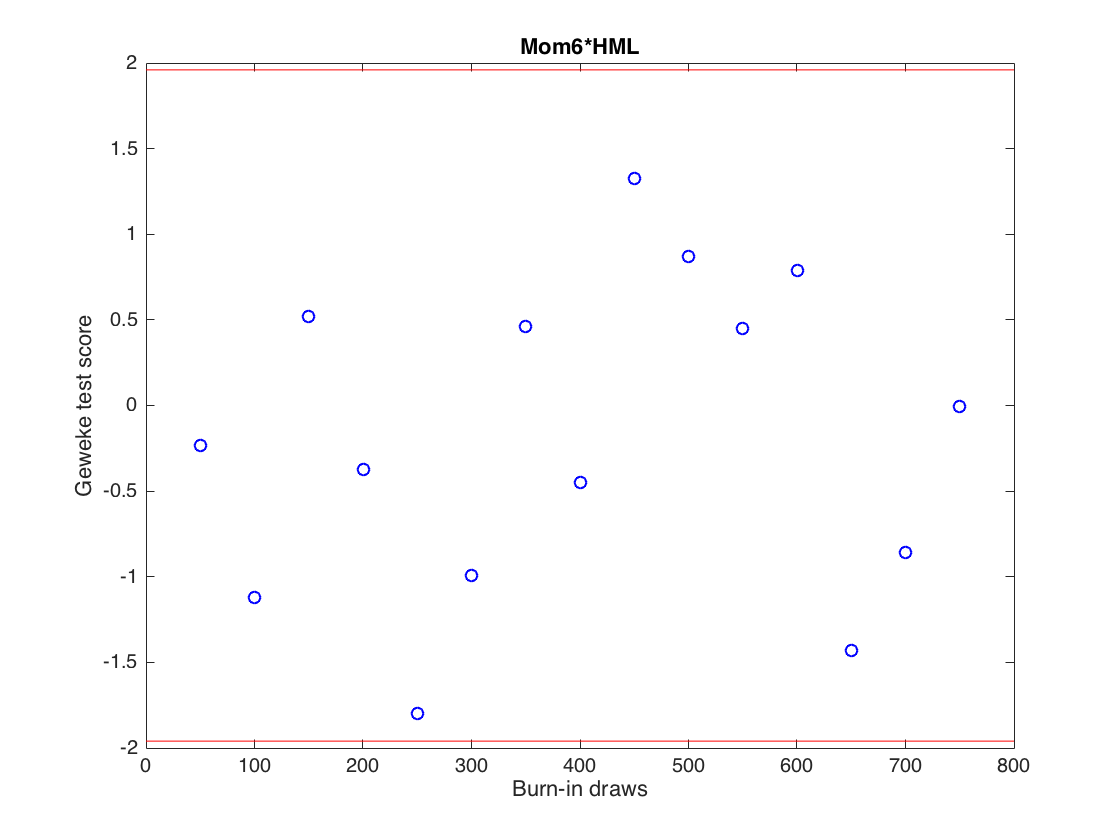
\includegraphics[width = 9cm, height = 7.5cm]{pictures/geweke1.png}
 
%     \end{subfigure}%
%     ~ 
%     \begin{subfigure}[b]{0.5\textwidth}
%         \centering
% \captionsetup{justification=centering,font=small,labelfont=footnotesize}
  
%         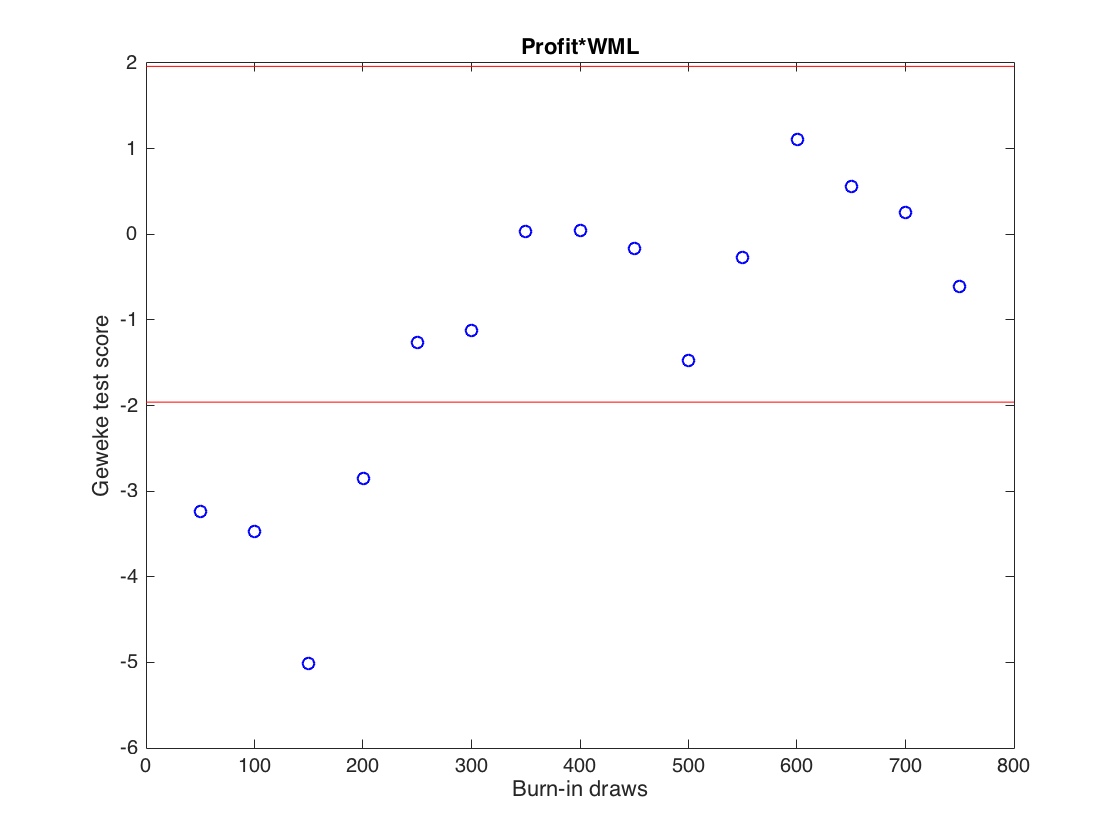
\includegraphics[width = 9cm, height = 7.5cm]{pictures/geweke2.png}
        
        

%     \end{subfigure}
    
%         \begin{subfigure}[b]{0.5\textwidth}
%         \centering 
%               \captionsetup{justification=centering, font=small,labelfont=footnotesize}
%         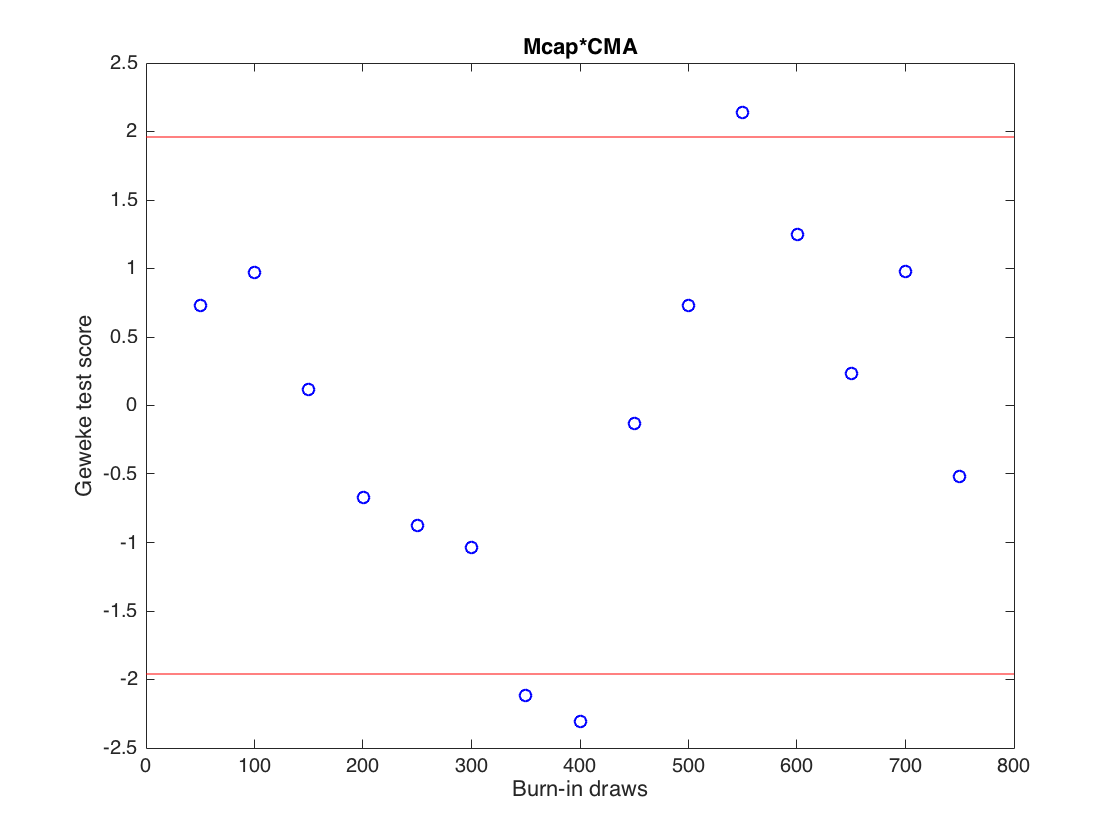
\includegraphics[width = 9cm, height = 7.5cm]{pictures/geweke3.png}
 
%     \end{subfigure}%
%     ~ 
%     \begin{subfigure}[b]{0.5\textwidth}
%         \centering
% \captionsetup{justification=centering,font=small,labelfont=footnotesize}
  
%         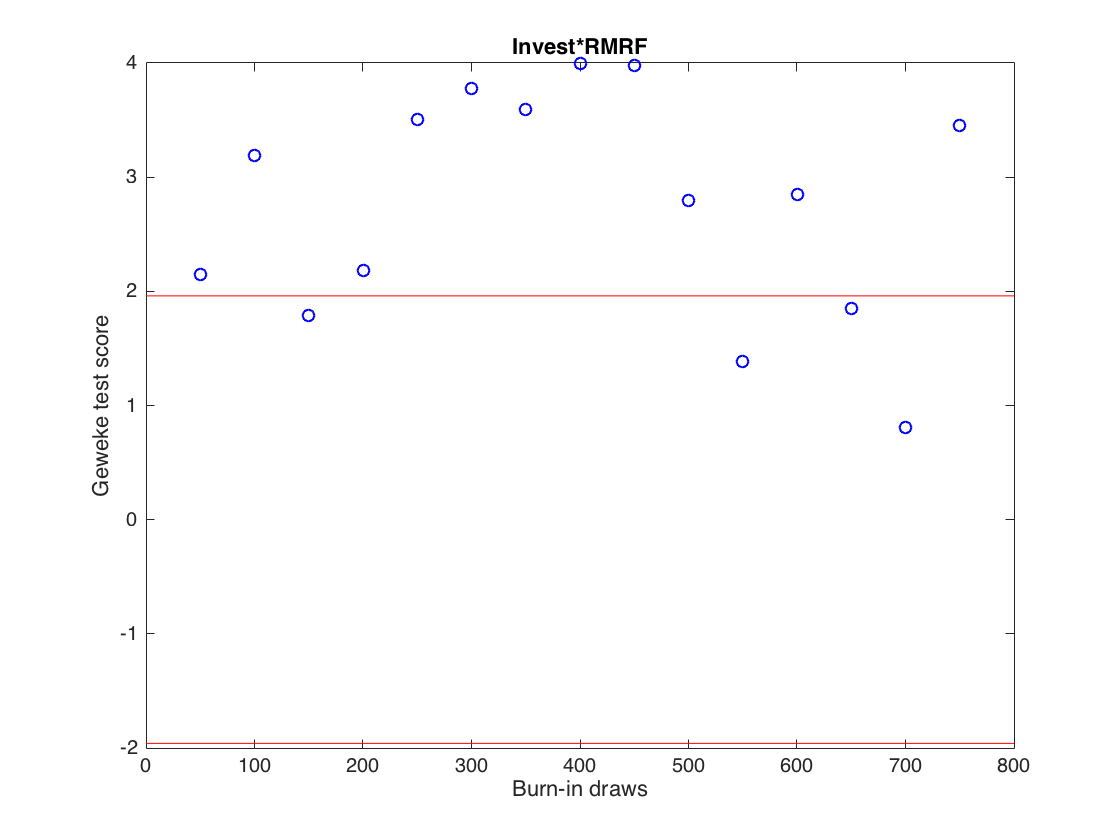
\includegraphics[width = 9cm, height = 7.5cm]{pictures/geweke4.png}
%             \end{subfigure}

% \end{figure}

% \subsubsection*{Derivation of full conditional posterior distributions}
% We provide the derivation of the full conditional posterior distributions of the parameters. The joint posterior distribution is written as 
% \begin{equation}
%     \label{posterior}
%     p(\Theta|R) \propto p(\Theta)p(R|\Theta).
% \end{equation}
% We can write the likelihood function of the data, $p(R|\Theta)$, as 
% \begin{equation}
%     p(R|\Theta) \propto \prod_{i=1}^{N} \frac{1}{\sigma^{T_i}_{\eta_i}} \text{exp}\left(-\frac{1}{2\sigma^2_{\eta_i}}(R_i-G_i\theta_i - H_i\xi)' (R_i-G_i\theta_i - H_i\xi)\right). 
% \end{equation}
%  We partition the set of model parameters $\Theta$ into separate blocks and derive the full conditional posterior distribution for each block. To derive the full conditional posterior for block $d$, that is, $d|\Theta_{-d},R$ with $\Theta_{-d}$ containing all parameters in $\Theta$ except $d$, we simply need to collect all the terms in $p(\Theta|R)$ depending on $d$. 
%  \par Regarding the fund-specific parameters $\theta_i$, we group all the terms in $p(\Theta|R)$ depending on $\theta_i$, such that we can derive the full conditional posterior distribution using the following steps


% \begin{alignat}{2}
% \label{proof1}
% p(\theta_i|\Theta_{-\theta_i},R) &\propto p(\theta_i)p(R|\Theta)  \nonumber  \\
%  &\propto \text{exp}\left(-\frac{1}{2}(\theta_i-\bar{\theta})'\Sigma^{-1}_{\theta} (\theta_i-\bar{\theta})\right) \text{exp}\left(-\frac{1}{2\sigma^2_{\eta_i}}(R_i-G_i\theta_i - H_i\xi)' (R_i-G_i\theta_i - H_i\xi)\right) \nonumber  \\ 
%       &= \text{exp}\left(-\frac{1}{2}\left[(\theta_i-\bar{\theta})'\Sigma^{-1}_{\theta} (\theta_i-\bar{\theta}) + \frac{1}{\sigma^2_{\eta_i}}(Y_i-G_i\theta_i)' (Y_i-G_i\theta_i )\right]\right)    \justif{\quad}{\text{Let} \hspace{0.1cm} 
%             Y_i = R_i - H_i\xi} \nonumber  \\ 
%              &= \text{exp}\left(-\frac{1}{2}\left[(\Sigma^{-\frac{1}{2}}_{\theta}\bar{\theta} - \Sigma^{-\frac{1}{2}}_{\theta} \theta_i)'(\Sigma^{-\frac{1}{2}}_{\theta}\bar{\theta} - \Sigma^{-\frac{1}{2}}_{\theta} \theta_i) + \frac{1}{\sigma^2_{\eta_i}}(Y_i-G_i\theta_i)' (Y_i-G_i\theta_i )\right]\right)                  \justif{\quad}{\text{Use} \hspace{0.1cm} [1]} \nonumber  \\
%   &=  \text{exp}\left(-\frac{1}{2}(w_i-V_i\theta_i)' (w_i-V_i\theta_i)\right)   \justif{\quad}{\text{Let} \hspace{0.15cm} w_i = \left[\frac{Y_i}{\sigma_{\eta_i}} \hspace{0.25cm} \Sigma^{-\frac{1}{2}}_{\theta}\bar{\theta} \right]' \hspace{0.15cm} \text{and} \hspace{0.15cm} V_i =  \left[\frac{G_i}{\sigma_{\eta_i}} \hspace{0.25cm} \Sigma^{-\frac{1}{2}}_{\theta} \right]'   } \nonumber   \\
%  &\propto \text{exp}\left(-\frac{1}{2}(\theta_i -\hat{\theta}_i)' V_i'V_i(\theta_i -\hat{\theta}_i)\right)     \justif{\quad}{\text{Use} \hspace{0.1cm} [2], \hspace{0.1cm} \text{with} \hspace{0.15cm} \hat{\theta}_i = (V_i'V_i)^{-1} V_iw_i, } \nonumber \\
% \end{alignat} 
% which is the kernel of a multivariate normal distribution, that is, the full conditional posterior distribution of $\theta_i$  is given by

% \begin{equation}
%     \theta_i|\Theta_{-\theta_i},R \sim \mathcal{N}\left(\tilde{\theta}_i,\tilde{\Sigma}_{\theta_i}\right), 
% \end{equation}
% with parameters
% \begin{equation}
%     \tilde{\theta}_i = \hat{\theta}_i = \tilde{\Sigma}_{\theta_i}\left(\frac{1}{\sigma^{2}_{\eta_i}}G_i'(R_i - H_i\xi) + \Sigma^{-1}_{\theta}\bar{\theta} \right) 
% \end{equation}
% \begin{equation}
%     \tilde{\Sigma}_{\theta_i} =  (V_i'V_i)^{-1} =\left(\frac{1}{\sigma^2_{\eta_i}}G_i'G_i +  \Sigma^{-1}_{\theta}\right)^{-1}. 
% \end{equation}
% Using the same steps as in \ref{proof1}, the full conditional posterior of $\bar{\theta}$ is given by 

%     \begin{equation}
%     \bar{\theta}|\Theta_{-\bar{\theta}},R \sim \mathcal{N}\left(\tilde{\bar{\theta}},\tilde{\Sigma}_{\bar{\theta}}\right),
% \end{equation}
% with parameters
% \begin{equation}
%     \tilde{\bar{\theta}} = \tilde{\Sigma}_{\bar{\theta}}\left(\Sigma^{-1}_{\theta} \sum^N_{i = 1} \theta_i + \Sigma^{-1}_{\mathit{k}} \mathit{k}\right) 
% \end{equation}
% \begin{equation}
%     \tilde{\Sigma}_{\bar{\theta}} =  \left(N \Sigma^{-1}_{\theta} +  \Sigma^{-1}_{\mathit{k}}\right)^{-1}. 
% \end{equation}

% \blfootnote{[1] Choleski decomposition: $B^{-1}$ = $B^{-\frac{1'}{2}}$$B^{-\frac{1}{2}}$.}
% \blfootnote{[2] Decomposition rule: $(y-X\beta)'(y-X\beta)$ = $(y-X\hat{\beta})'(y-X\hat{\beta})$ + $(\beta - \hat{\beta})'X'X(\beta - \hat{\beta})$,  where $\hat{\beta}$ = $(X'X)^{-1}X'y$. }
% \blfootnote{[3] Product of determinants: $|A||B|$ = $|AB|$.}
% \blfootnote{[4] Trace of a scalar: $A$ = Tr($A$), where $A$ is a scalar.}
% \blfootnote{[5] Invariance of the trace under cyclic permutations: Tr$(ABC)$ = Tr($CAB$) = Tr($BCA$).}
% \blfootnote{[6] Sum of traces: Tr($A$) + Tr($B$) = Tr($A$+$B$).}

% \noindent Regarding the covariance matrix $\Sigma_{\theta}$, we derive the full conditional posterior as follows

% \begin{alignat}{2}
% p(\Sigma_{\theta}|\Theta_{-\Sigma_{\theta}},R) &\propto p(\Sigma_{\theta}) \prod^N_{i=1}p(\theta_i)  \nonumber  \\
%  &\propto |\Sigma_{\theta}|^{-\frac{\psi_{\theta} + k + 1}{2}}  \text{exp}\left(-\frac{1}{2}\text{tr}(\Sigma^{-1}_{\theta} \psi_{\theta}S_{\theta})\right) \prod^N_{i=1} |\Sigma_{\theta}|^{-\frac{1}{2}}  \text{exp}\left(-\frac{1}{2}(\theta_i - \bar{\theta})' \Sigma^{-1}_{\theta}(\theta_i - \bar{\theta})\right) \nonumber  \\ 
%       &= 
%       |\Sigma_{\theta}|^{-\frac{\psi_{\theta} + N+k + 1}{2}} \text{exp}\left(-\frac{1}{2}\left[\text{tr}(\Sigma^{-1}_{\theta} \psi_{\theta}S_{\theta}) + \text{tr}\left(\sum^N_{i=1}(\theta_i - \bar{\theta})' \Sigma^{-1}_{\theta}(\theta_i - \bar{\theta}) \right) \right]\right)    \justif{\quad}{\text{Use}\hspace{0.1cm} [3]+[4]} \nonumber  \\ 
% &= 
%       |\Sigma_{\theta}|^{-\frac{\psi_{\theta} + N+k + 1}{2}} \text{exp}\left(-\frac{1}{2}\left[\text{tr}( \Sigma^{-1}_{\theta} \psi_{\theta}S_{\theta}) + \text{tr}\left(\sum^N_{i=1}\Sigma^{-1}_{\theta}(\theta_i - \bar{\theta})(\theta_i - \bar{\theta})' \right) \right]\right)    \justif{\quad}{\text{Use}\hspace{0.1cm} [5]} \nonumber  \\ 
% &= 
%       |\Sigma_{\theta}|^{-\frac{\psi_{\theta} + N+k + 1}{2}} \text{exp}\left(-\frac{1}{2}\text{tr}\left(  \Sigma^{-1}_{\theta} \left[\sum^N_{i=1}(\theta_i - \bar{\theta}) (\theta_i - \bar{\theta})' +  \psi_{\theta}S_{\theta} \right]\right)\right)    \justif{\quad}{\text{Use}\hspace{0.1cm} [6]}, \nonumber  \\ 
% \end{alignat} 
% which is the kernel of an inverted Wishart distribution, that is, the full conditional posterior distribution of $\Sigma_{\theta}$ is given by 
% \begin{equation}
%     \Sigma_{\theta}|\Theta_{-\Sigma_{\theta}},R \sim \mathit{IW}\left(\sum^N_{i=1}(\theta_i-\bar{\theta})(\theta_i-\bar{\theta})'+\psi_{\theta}S_{\theta},\psi_{\theta} + N\right)
% \end{equation}
% Using the same steps as in \ref{proof1}, the full conditional posterior of $\xi$ is given by
% \begin{equation}
%     \xi|\Theta_{-\xi} \sim \mathcal{N}(\tilde{\xi},\tilde{\Sigma}_{\xi}),
% \end{equation}
% with parameters 

% \begin{equation}
%     \tilde{\xi} = \tilde{\Sigma}_{\xi}\left(\sum^N_{i=1}\frac{1}{\sigma^2_{\eta_i}} H_i'(R_i - G_i\theta_i) + \Sigma^{-1}_{\xi} \bar{\xi}\right) 
% \end{equation}

% \begin{equation}
%     \tilde{\Sigma}_{\xi} =  \left(\sum^N_{i=1}\frac{1}{\sigma^2_{\eta_i}}  H_i'H_i + \Sigma^{-1}_{\xi}\right)^{-1}. 
% \end{equation}
% Finally, we derive the full conditional posterior of $\sigma^2_{\eta_i}$ as follows 

% \begin{alignat}{2}
% p(\sigma^2_{\eta_i}|\Theta_{-\Sigma_{\sigma^2_{\eta_i}}},R) &\propto p(\sigma^2_{\eta_i})p(R|\Theta)  \nonumber  \\
%  &\propto \sigma^{-(T_i+2)}_{\eta_i}  \text{exp}\left(-\frac{1}{2\sigma^2_{\eta_i}}(R_i - G_i\theta_i -H_i\xi)'(R_i - G_i\theta_i -H_i\xi)\right), \nonumber  \\ 
% \end{alignat} 
% which is the kernel of an inverted Gamma-2 distribution, that is, the full conditional posterior distribution of $\sigma^2_{\eta_i}$ is given by 
% \begin{equation}
%     \sigma^2_{\eta_i}|\Theta_{-\sigma^2_{\eta_i}} \sim \mathit{IG}2\left((R_i - G_i\theta_i -H_i\xi)'(R_i - G_i\theta_i -H_i\xi),T_i\right).
% \end{equation}
% \begin{table}[H]
% \centering
% \small
% \centering
% \setlength{\tabcolsep}{21pt}
% {\captionsetup{justification=centering,singlelinecheck=off}
% \caption*{\bfseries Table A2: Four-factor model alpha vs fund-level charactersistics }}
% \caption*{This table presents the time-series averages of coefficients ($c$) from monthly regressions,
% \begin{equation*}
% \label{a}
%     \alpha_{it} = c_{0t} + c_{1t}Z_{it-1} + u_i.
% \end{equation*}
% We employ the \citet{carhart1997persistence} four-factor model. The alphas ($\alpha_{it})$ are estimated with OLS from rolling time series using returns from time $t$-35 until $t$. The fund characteristics (Z) are the logarithm of the market capitalization (Mcap), the logarithm of the book-to-market ratio (B/M), and the logarithm of one plus the cumulative past six-month cumulative return (Mom6). We calculate fund-level characteristics by a portfolio-weighted average across individual fund holdings. Each fund-level characteristic is winsorized at the 0.5\% and the 99.5\% levels. We also standardize each fund-level characteristic by subtracting its monthly cross-sectional mean. Panel A reports average four-factor alphas in quintiles sorted on characteristics. T-statistics with the \citet{newey1986simple} correction of 12 lags are in parenthesis. Significant alphas at the 5\% level are in bold font. Panel B reports the average coefficients from the monthly regressions. \citet{fama1973risk} t-statistics with the \citet{newey1986simple} correction of 12 lags are in parenthesis. Estimates significant at the 5\% level are in bold font. The sample period is April 1983 to December 2015.   }
% {\captionsetup{justification=centering,singlelinecheck=off}
% \caption*{Panel A: Average four-factor alpha in quintiles sorted on characteristics  }
% \begin{tabular}{crrr}
% \hline
% Quintile & \multicolumn{1}{c}{Mcap} & \multicolumn{1}{c}{B/M} & \multicolumn{1}{c}{Mom6} \\ \hline
% 1        & -0.044                   & -0.015                  & \textbf{-0.065}          \\
%          & (-1.49)                  & (-0.51)                 & (-3.10)                  \\
% 2        & 0.001                    & -0.048                  & -0.045                   \\
%          & (0.02)                   & \textbf{(-2.06)}        & \textbf{(-2.81)}         \\
% 3        & -0.037                   & -0.041                  & -0.038                   \\
%          & (1.85)                   & (-2.21)                 & (-2.13)                  \\
% 4        & \textbf{-0.059}          & \textbf{-0.049}         & -0.035                   \\
%          & (-4.06)                  & (-2.70)                 & (-1.66)                  \\
% 5        & \textbf{-0.074}          & \textbf{-0.060}         & -0.020                   \\
%          & (-6.39)                  & (-2.64)                 & (-0.78)                  \\
% 5-1      & -0.030                   & -0.045                  & \textbf{0.045}           \\
%          & (-1.09)                  & (-1.36)                 & (2.34)                   \\ \hline
% \end{tabular}
% \end{table}

% \begin{table}[H]
% \centering
% \small
% \setlength{\tabcolsep}{15.5pt}
% {\captionsetup{justification=centering,singlelinecheck=off}
% \caption*{ Panel B: Cross-sectional regressions of four-factor alpha on characteristics }}
% \begin{tabular}{crrrr}
% \hline
% Cnt  & \textbf{-0.042} & \textbf{-0.042} & \textbf{-0.042} & \textbf{-0.042} \\ \hline
%      & (-2.20)         & (-2.20)         & (-2.20)         & (-2.20)         \\
% Mcap & -0.003          &                 &                 & -0.002          \\
%      & (-1.77)         &                 &                 & (-1.14)         \\
% B/M  &                 & -0.049          &                 & -0.023          \\
%      &                 & (-0.72)         &                 & (-0.36)         \\
% Mom6 &                 &                 & \textbf{0.003}  & 0.001           \\
%      &                 &                 & (2.03)          & (1.26)          \\ \hline
% \end{tabular}
% \end{table}


% \begin{table}[H]
% \centering
% \small
% \centering
% \setlength{\tabcolsep}{24pt}
% {\captionsetup{justification=centering,singlelinecheck=off}
% \caption*{\bfseries Table A3: DGTW characteristic selectivity measure vs four-factor fund betas}}
% \caption*{This table presents the time-series averages of coefficients ($c$) from monthly regressions,
% \begin{equation*}
% \label{a}
%     \text{DGTW}_{i,t-35:t} = c_{0t} + c_{1t}\hat{B}_{it} + u_i.
% \end{equation*}
% We employ the characteristic selectivity (CS) measure of Daniel, Grinblatt, Titman, and Wermens (DGTW; 1997). The dependent variable $\text{DGTW}_{i,t-35:t}$ is the time series average of the DGTW CS measure over the period from time $t$-35 until $t$. Using fund returns over this period, we estimate the factor betas ($\hat{B}_{it}$) from the four-factor model of \citet{carhart1997persistence}. We standardize each factor beta by subtracting its monthly cross-sectional mean. Panel A reports the average DGTW CS measure in quintiles sorted on factor betas. T-statistics with the \citet{newey1986simple} correction of 12 lags are in parenthesis. Significant DGTW CS measures at the 5\% level are in bold font. Panel B reports the average coefficients from the monthly regressions. \citet{fama1973risk} t-statistics with the \citet{newey1986simple} correction of 12 lags are in parenthesis. Estimates significant at the 5\% level are in bold font. The sample period is April 1983 to December 2015.  }
% {\captionsetup{justification=centering,singlelinecheck=off}
% \caption*{Panel A: Average DGTW CS measure in quintiles sorted on four-factor betas  }
% \begin{tabular}{crrr}
% \hline
% Quintile & SMB            & HML            & WML             \\ \hline
% 1        & \textbf{0.021} & 0.038          & \textbf{-0.049} \\
%          & (2.26)         & (1.38)         & (-3.16)         \\
% 2        & 0.004          & 0.014          & 0.005           \\
%          & (0.47)         & (1.31)         & (0.44)          \\
% 3        & \textbf{0.025} & \textbf{0.025} & \textbf{0.028}  \\
%          & (2.39)         & (2.93)         & (3.42)          \\
% 4        & \textbf{0.049} & \textbf{0.028} & \textbf{0.053}  \\
%          & (4.58)         & (2.13)         & (6.76)          \\
% 5        & 0.053          & 0.028          & \textbf{0.096}  \\
%          & (1.91)         & (1.47)         & (5.46)          \\
% 5-1      & 0.032          & -0.053         & \textbf{0.052}  \\
%          & (1.74)         & (-0.23)        & (6.33)          \\ \hline
% \end{tabular}
% \end{table}

% \begin{table}[H]
% \centering
% \small
% \setlength{\tabcolsep}{12pt}
% {\captionsetup{justification=centering,singlelinecheck=off}
% \caption*{ Panel B: Cross-sectional regressions of DGTW CS measure on four-factor betas}}
% \label{my-label}
% \begin{tabular}{crrrrr}
% \hline
% Cnt  & \textbf{0.027} & \textbf{0.027} & \textbf{0.027} & \textbf{0.027} & \textbf{0.027} \\
%      & (3.25)         & (3.25)         & (3.25)         & (3.25)         & (3.25)         \\
% RMRF & -0.031         &                &                &                & -0.073         \\
%      & (-0.50)        &                &                &                & (-1.42)        \\
% SMB  &                & 0.067          &                &                & 0.036          \\
%      &                & (1.93)         &                &                & (1.64)         \\
% HML  &                &                & -0.002         &                & 0.003          \\
%      &                &                & (-0.04)        &                & (0.07)         \\
% WML  &                &                &                & \textbf{0.364} & \textbf{0.347} \\
%      &                &                &                & (7.73)         & (10.17)        \\ \hline
% \end{tabular}
% \end{table}

% \begin{table}[H]
% \small
% {\captionsetup{justification=centering,singlelinecheck=off}
% \caption*{\bfseries Table A2: Mutual Fund Performance Persistence }}
% \caption*{This table presents returns of decile porfolios sorted by the \citet{carhart1997persistence} four-factor model alpha (Panel A), double-adjusted four-factor alpha (Panel B) and characteristic-driven performance (Panel C). These performance measured are calculated using rolling windows with a window size of 36 months. Portfolios are rebalanced every quarter-end and are held for up to six years. To deal with overlapping portfolios, we follow \citet{jegadeesh1993returns} to take the equal-weighted return across overlapping portfolios formed in different quarters. Two different returns are reported: the excess return over the risk-free rate and the four-factor alpha. T-statistics, shown in parenthesis, are computed using White's standard errors. Estimated significant at the 5\% level are in bold font. The sample period is May 1980 to December 2015.}
% \label{my-label}
% \begin{tabular}{cccccccccccc}
% \hline
%       & \multicolumn{2}{c}{Qtr 1} &  & \multicolumn{2}{c}{Qtr 1-4} &  & \multicolumn{2}{c}{Qtr 5-12} &  & \multicolumn{2}{c}{Qtr 13-24} \\ \cline{2-3} \cline{5-6} \cline{8-9} \cline{11-12} 
% Decile & Excess     & 4F alpha     &  & Excess      & 4F alpha      &  & Excess       & 4F alpha      &  & Excess       & 4F alpha       \\ \hline
% \multicolumn{12}{l}{Panel A: Carhart four-factor alpha}                                                                                          \\
% 1      & 0.52       & -0.16        &  & 0.56        & -0.15         &  & 0.56         & -0.14         &  & 0.48         & -0.15          \\
% 2      & 0.55       & -0.09        &  & 0.54        & -0.12         &  & 0.55         & -0.10         &  & 0.52         & -0.09          \\
% 3      & 0.56       & -0.08        &  & 0.55        & -0.09         &  & 0.56         & -0.08         &  & 0.55         & -0.07          \\
% 4      & 0.53       & -0.10        &  & 0.56        & -0.08         &  & 0.55         & -0.08         &  & 0.53         & -0.08          \\
% 5      & 0.58       & -0.07        &  & 0.57        & -0.07         &  & 0.55         & -0.09         &  & 0.50         & -0.11          \\
% 6      & 0.57       & -0.07        &  & 0.58        & -0.06         &  & 0.54         & -0.09         &  & 0.53         & -0.08          \\
% 7      & 0.60       & -0.04        &  & 0.58        & -0.05         &  & 0.55         & -0.06         &  & 0.53         & -0.08          \\
% 8      & 0.59       & -0.05        &  & 0.60        & -0.03         &  & 0.56         & -0.05         &  & 0.52         & -0.08          \\
% 9      & 0.62       & -0.02        &  & 0.61        & -0.02         &  & 0.55         & -0.06         &  & 0.53         & -0.08          \\
% 10     & 0.71       & 0.03         &  & 0.66        & 0.01          &  & 0.60         & -0.03         &  & 0.57         & -0.07          \\
% 10-1  & 0.19       & 0.20         &  & 0.11        & 0.16          &  & 0.04         & 0.11          &  & 0.09         & 0.08           \\
%       & (\bf{3.47})       & (\bf{3.49})         &  & (\bf{2.32})        & (\bf{3.21})         &  & (\bf{0.73})         & (\bf{2.01})          &  & (1.69)         & (1.73)           \\
%       &            &              &  &             &               &  &              &               &  &              &                \\
% \multicolumn{12}{l}{Panel B: Double-adjusted Carhart four-factor alpha}                                                                          \\
% 1      & 0.56       & -0.14        &  & 0.57        & -0.14         &  & 0.54         & -0.14         &  & 0.47         & -0.16          \\
% 2      & 0.56       & -0.08        &  & 0.56        & -0.10         &  & 0.55         & -0.10         &  & 0.53         & -0.09          \\
% 3      & 0.54       & -0.11        &  & 0.57        & -0.09         &  & 0.56         & -0.09         &  & 0.53         & -0.09          \\
% 4      & 0.57       & -0.07        &  & 0.58        & -0.07         &  & 0.55         & -0.09         &  & 0.52         & -0.09          \\
% 5      & 0.59       & -0.05        &  & 0.56        & -0.07         &  & 0.54         & -0.09         &  & 0.52         & -0.09          \\
% 6      & 0.57       & -0.07        &  & 0.57        & -0.06         &  & 0.55         & -0.07         &  & 0.52         & -0.08          \\
% 7      & 0.58       & -0.05        &  & 0.57        & -0.06         &  & 0.55         & -0.06         &  & 0.53         & -0.08          \\
% 8      & 0.57       & -0.07        &  & 0.59        & -0.04         &  & 0.55         & -0.06         &  & 0.51         & -0.09          \\
% 9      & 0.63       & -0.01        &  & 0.61        & -0.03         &  & 0.57         & -0.04         &  & 0.55         & -0.06          \\
% 10     & 0.67       & 0.01         &  & 0.64        & -0.01         &  & 0.59         & -0.04         &  & 0.57         & -0.06          \\
% 10-1  & 0.11       & 0.15         &  & 0.07        & 0.13          &  & 0.05         & 0.11          &  & 0.10         & 0.10           \\
%       & (\textbf{3.10})       & (\textbf{4.13})         &  & (\textbf{2.39})        & (\textbf{4.23})          &  & (1.34)         & (\textbf{2.94})          &  & (\textbf{2.56})         & (\textbf{3.31})           \\
%       &            &              &  &             &               &  &              &               &  &              &                \\
% \multicolumn{12}{l}{Panel C: Characteristic-driven performance}                                                                       \\
% 1      & 0.49       & -0.11        &  & 0.54        & -0.11         &  & 0.61         & -0.06         &  & 0.53         & -0.09          \\
% 2      & 0.53       & -0.08        &  & 0.57        & -0.07         &  & 0.60         & -0.05         &  & 0.54         & -0.07          \\
% 3      & 0.53       & -0.09        &  & 0.56        & -0.08         &  & 0.57         & -0.07         &  & 0.54         & -0.06          \\
% 4      & 0.55       & -0.07        &  & 0.57        & -0.06         &  & 0.56         & -0.08         &  & 0.52         & -0.08          \\
% 5      & 0.57       & -0.06        &  & 0.59        & -0.04         &  & 0.56         & -0.07         &  & 0.54         & -0.07          \\
% 6      & 0.60       & -0.06        &  & 0.60        & -0.06         &  & 0.55         & -0.08         &  & 0.52         & -0.09          \\
% 7      & 0.62       & -0.06        &  & 0.58        & -0.08         &  & 0.54         & -0.10         &  & 0.52         & -0.10          \\
% 8      & 0.62       & -0.05        &  & 0.59        & -0.06         &  & 0.53         & -0.10         &  & 0.52         & -0.10          \\
% 9      & 0.64       & -0.03        &  & 0.60        & -0.06         &  & 0.52         & -0.09         &  & 0.51         & -0.11          \\
% 10     & 0.70       & -0.02        &  & 0.61        & -0.06         &  & 0.53         & -0.08         &  & 0.54         & -0.10          \\
% 10-1  & 0.20       & 0.10         &  & 0.06        & 0.06          &  & -0.09        & -0.01         &  & 0.01         & -0.01          \\
%       & (1.58)       & (0.80)         &  & (0.61)        & (0.60)         &  & (-0.89)        & (-0.14)         &  & (0.15)         & (-0.12)          \\ \hline
% \end{tabular}
% \end{table}





\end{document}
